\documentclass[10pt,twoside,openright]{memoir}

%% General

\usepackage{afterpage}
\usepackage{makeidx}
\makeindex

\usepackage[normalem]{ulem}

%% BEGIN Dimensions

%% Set the stock size (document dimensions)
\setstocksize{9.25in}{7.5in}

%% Force trim to same size as stock - i.e. the document is the same size as the
%% final output with no bleed or trimming.
\settrimmedsize{\stockheight}{\stockwidth}{*}

%% Set spine margin to 0.8in, and ensure that fore-edge margin is 1.5 * the size
\setlrmarginsandblock{0.8in}{*}{1.5}
\setulmarginsandblock{1in}{1.2in}{*}
\checkandfixthelayout 

%% END Dimensions

\setlength{\parindent}{0em}
\nonzeroparskip

\usepackage{xcolor}
\usepackage{enumitem}
\usepackage{longtable}
\usepackage{newtxmath}
\definecolor{verylightgray}{cmyk}{0, 0, 0, 0.1}
\definecolor{mediumgray}{cmyk}{0, 0, 0, 0.4}

\usepackage[most]{tcolorbox}
\newtcolorbox[auto counter,number within=section]{notice}[1][]{
  enhanced jigsaw,colback=white,colframe=gray,coltitle=black,
  fonttitle=\bfseries\sffamily,
  sharp corners,
  detach title,
  leftrule=12mm,
  % What you need %%%%%%%%%%%%
  underlay unbroken and first={\node[below,text=black,anchor=east]
  at ([xshift=-10pt]interior.base west) {\Huge\textbf{\textcolor{white}{$\lambdaup$}}};},
  %%%%%%%%%%%%%%%%%%%%%%%%
  %breakable,pad at break=1mm,
  #1,
  code={\ifdefempty{\tcbtitletext}{}{\tcbset{before upper={\tcbtitle\par\medskip}}}},
}

%% Graphics
\usepackage{graphicx}
\usepackage{float}
\graphicspath{ {./images/} }
\usepackage[export]{adjustbox}

%% Code Listings
\usepackage{listings}
\lstset{
    basicstyle=\footnotesize\ttfamily, % Default font
    %% numbers=left,              % Location of line numbers
    %% numberstyle=\tiny,          % Style of line numbers
    %% stepnumber=1,              % Margin between line numbers
    %% numbersep=5pt,              % Margin between line numbers and text
    tabsize=2,                  % Size of tabs
    extendedchars=true,
    breaklines=true,            % Lines will be wrapped
    keywordstyle=\textbf,
    frame=b,
    showspaces=false,
    showtabs=false,
    xleftmargin=5pt,
    framexleftmargin=5pt,
    framexrightmargin=5pt,
    framexbottommargin=4pt,
%    framesep=10pt,
    backgroundcolor=\color{verylightgray},
    escapechar=\%,
    % showstringspaces=false
}
\setlength\abovecaptionskip{-5pt}

\lstdefinelanguage{JavaScript}{
  keywords={break, case, catch, continue, const, debugger, default, delete, do, else, finally, for, function, if, in, instanceof, let, new, of, return, switch, this, throw, try, typeof, var, void, while, with},
  morecomment=[l]{//},
  morecomment=[s]{/*}{*/},
  morestring=[b]',
  morestring=[b]",
  sensitive=true
}
\lstdefinelanguage{Clojure}{
  keywords={def defn},
  morecomment=[l]{;;},
  morestring=[b]",
  sensitive=true
}
\lstdefinelanguage{CSS}{
      keywords={accelerator,azimuth,background,background-attachment,
            background-color,background-image,background-position,
            background-position-x,background-position-y,background-repeat,
            behavior,border,border-bottom,border-bottom-color,
            border-bottom-style,border-bottom-width,border-collapse,
            border-color,border-left,border-left-color,border-left-style,
            border-left-width,border-right,border-right-color,
            border-right-style,border-right-width,border-spacing,
            border-style,border-top,border-top-color,border-top-style,
            border-top-width,border-width,bottom,caption-side,clear,
            clip,color,content,counter-increment,counter-reset,cue,
            cue-after,cue-before,cursor,direction,display,elevation,
            empty-cells,filter,float,font,font-family,font-size,
            font-size-adjust,font-stretch,font-style,font-variant,
            font-weight,height,ime-mode,include-source,
            layer-background-color,layer-background-image,layout-flow,
            layout-grid,layout-grid-char,layout-grid-char-spacing,
            layout-grid-line,layout-grid-mode,layout-grid-type,left,
            letter-spacing,line-break,line-height,list-style,
            list-style-image,list-style-position,list-style-type,margin,
            margin-bottom,margin-left,margin-right,margin-top,
            marker-offset,marks,max-height,max-width,min-height,
            min-width,-moz-binding,-moz-border-radius,
            -moz-border-radius-topleft,-moz-border-radius-topright,
            -moz-border-radius-bottomright,-moz-border-radius-bottomleft,
            -moz-border-top-colors,-moz-border-right-colors,
            -moz-border-bottom-colors,-moz-border-left-colors,-moz-opacity,
            -moz-outline,-moz-outline-color,-moz-outline-style,
            -moz-outline-width,-moz-user-focus,-moz-user-input,
            -moz-user-modify,-moz-user-select,orphans,outline,
            outline-color,outline-style,outline-width,overflow,
            overflow-X,overflow-Y,padding,padding-bottom,padding-left,
            padding-right,padding-top,page,page-break-after,
            page-break-before,page-break-inside,pause,pause-after,
            pause-before,pitch,pitch-range,play-during,position,quotes,
            -replace,richness,right,ruby-align,ruby-overhang,
            ruby-position,-set-link-source,size,speak,speak-header,
            speak-numeral,speak-punctuation,speech-rate,stress,
            scrollbar-arrow-color,scrollbar-base-color,
            scrollbar-dark-shadow-color,scrollbar-face-color,
            scrollbar-highlight-color,scrollbar-shadow-color,
            scrollbar-3d-light-color,scrollbar-track-color,table-layout,
            text-align,text-align-last,text-decoration,text-indent,
            text-justify,text-overflow,text-shadow,text-transform,
            text-autospace,text-kashida-space,text-underline-position,top,
            unicode-bidi,-use-link-source,vertical-align,visibility,
            voice-family,volume,white-space,widows,width,word-break,
            word-spacing,word-wrap,writing-mode,z-index,zoom},  
      sensitive=true,
      morecomment=[l]{//},
      morecomment=[s]{/*}{*/},
      morestring=[b]',
      morestring=[b]",
      alsoletter={:},
      alsodigit={-}
    }

\usepackage{tikz}
\usetikzlibrary{shadows}

\newcommand*\circled[1]{\tikz[baseline=(char.base)]{
            \node[shape=circle,draw,inner sep=1pt] (char) {#1};}}

\newcommand*\keystroke[1]{%
  \tikz[baseline=(key.base)]
    \node[%
      draw,
      fill=white,
      drop shadow={shadow xshift=0.25ex,shadow yshift=-0.25ex,fill=black,opacity=0.75},
      rectangle,
      rounded corners=2pt,
      inner sep=1pt,
      line width=0.5pt,
      font=\scriptsize\sffamily
    ](key) {#1\strut}
  ;
}

\usepackage{caption}
\DeclareCaptionFont{white}{\color{white}}
\DeclareCaptionFormat{listing}{\colorbox{mediumgray}{\parbox{\textwidth}{\hspace{5pt}#1#2#3}}}
\captionsetup[lstlisting]{format=listing,labelfont=white,textfont=white, singlelinecheck=false, margin=0pt, font={sf,bf,footnotesize}}

%% Metadata
\author{Andrew Meredith}
\title{Learn ClojureScript}
\newcommand{\subTitle}{Functional programming for the web}

%% Fonts

\usepackage{fontspec}
\usepackage{microtype}
\setmainfont[
    Path = fonts/PT_Serif/,
    BoldFont = PTSerif-Bold,
    ItalicFont = PTSerif-Italic,
    BoldItalicFont = PTSerif-BoldItalic
]{PTSerif-Regular}
\setsansfont[
    Path = fonts/Oswald/,
    BoldFont = Oswald-Bold,
    ItalicFont = Oswald-Light,% not actual italic font
    BoldItalicFont = Oswald-SemiBold% not actual italic font
]{Oswald-Regular}
\setmonofont[
    Path = fonts/Fira_Code/,
    Scale = 0.7,
    BoldFont = FiraCode-Bold
]{FiraCode-Regular}
\usepackage[sf, raggedright]{titlesec}

%% Quotes

%%%%********************************************************************
% fancy quotes
\definecolor{quotemark}{gray}{0.7}
\makeatletter
\def\fquote{%
    \@ifnextchar[{\fquote@i}{\fquote@i[]}%]
           }%
\def\fquote@i[#1]{%
    \def\tempa{#1}%
    \@ifnextchar[{\fquote@ii}{\fquote@ii[]}%]
                 }%
\def\fquote@ii[#1]{%
    \def\tempb{#1}%
    \@ifnextchar[{\fquote@iii}{\fquote@iii[]}%]
                      }%
\def\fquote@iii[#1]{%
    \def\tempc{#1}%
    \vspace{1em}%
    \noindent%
    \begin{list}{}{%
         \setlength{\leftmargin}{0.1\textwidth}%
         \setlength{\rightmargin}{0.1\textwidth}%
                  }%
         \item[]%
         \begin{picture}(0,0)%
         \put(-15,-5){\makebox(0,0){\scalebox{3}{\textcolor{quotemark}{``}}}}%
         \end{picture}%
         \begingroup\itshape}%
 %%%%********************************************************************
 \def\endfquote{%
 \endgroup\par%
 \makebox[0pt][l]{%
 \hspace{0.8\textwidth}%
 \begin{picture}(0,0)(0,0)%
 \put(15,15){\makebox(0,0){%
 \scalebox{3}{\color{quotemark}''}}}%
 \end{picture}}%
 \ifx\tempa\empty%
 \else%
    \ifx\tempc\empty%
       \hfill\rule{100pt}{0.5pt}\\\mbox{}\hfill\tempa,\ \emph{\tempb}%
   \else%
       \hfill\rule{100pt}{0.5pt}\\\mbox{}\hfill\tempa,\ \emph{\tempb},\ \tempc%
   \fi\fi\par%
   \vspace{0.5em}%
 \end{list}%
 }%
 \makeatother
 %%%%********************************************************************

%% BEGIN TITLE

\makeatletter
\def\maketitle{%
  \null
  \thispagestyle{empty}%
  %%\vfill
  \begin{center}\leavevmode
    \begin{flushright}
    \normalfont
    {\Huge\textbf{\textsf{\@title}}\par}%
    \hrulefill\par
    {\LARGE\textsf{\subTitle}\par}%
    \vskip 4.5cm
    {\LARGE\textbf{\@author}\par}%
    \vskip 4.5cm
    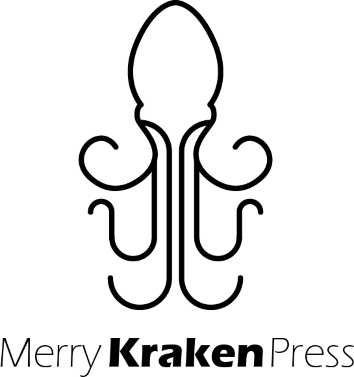
\includegraphics[right]{merry-kraken-bw}
    \end{flushright}
  \end{center}%
  \vfill
  \null
  \cleardoublepage
  }
\makeatother
\date{}


\renewcommand{\chaptername}{Lesson}


%%% BEGIN DOCUMENT

\begin{document}

\maketitle

\frontmatter

\null\vfill

\begin{flushleft}
\textit{Learn ClojureScript: Functional programming for the web}


© Copyright 2021 by Andrew Meredith.


ISBN--13: 978-1-7367172-0-2

\bigskip
All rights reserved. With the exception of the code examples, no part of this book may be reproduced in any form by any electronic or mechanical means (including photocopying, recording, or information storage and retrieval) without permission in writing (whether in physical or signed electronic form) from the publisher. All code examples are licensed under a \emph{Creative Commons Attribution 4.0 International License (CC BY 4.0)}. See \texttt{https://creativecommons.org/licenses/by/4.0/} for details. Permission is hereby granted to reproduce any portion of this book for any and all educational uses. For all other uses, permission may be obtained by submitting an electronic request via email to \texttt{publisher@learn-clojurescript.com} or a written request to:

\bigskip
Merry Kraken Press\linebreak
Attn: Publisher\linebreak
10470 Holly Springs Pl.\linebreak
Peyton, CO 80831\linebreak

\bigskip
Typeset using XeLaTeX, based on the memoir class. PT Serif was used as the primary body font, Oswald for headings and captions, and Fira Code for code listings and verbatim text.

\end{flushleft}

\clearpage

\thispagestyle{empty}%
\begin{flushright}
\normalfont
{\Large\textbf{\textsf{Praise for \emph{Learn ClojureScript}}}\par}%
\hrulefill\par
\vskip 2cm

\begin{fquote}[Brandon Bloom][CEO, Deref Inc.]Discovering Clojure has had a profound impact on my career, forever changing how I think about programming. \emph{Learn ClojureScript} offers a smooth onramp and a good mix of both the practical and theoretical aspects of the language. With this book, web developers of all experience levels can enjoy their Clojure eureka moments while building on fun and interesting examples.
\end{fquote}

\begin{fquote}[Kelvin Mai][Full-Stack Engineer]\emph{Learn ClojureScript} covers everything necessary without being overwhelming. The book is perfect for beginners to the language, and it's a resource I wished was around when I got into the world of Clojure and ClojureScript.
\end{fquote}

\begin{fquote}[Roger Erens][Software Engineer]This is the gentlest introduction that the ClojureScript ecosystem offers. The capstone projects give you what you need to get a ClojureScript frontend up and running.
\end{fquote}


\end{flushright}
\vfill

\cleardoublepage

\tableofcontents

\cleardoublepage

%\normalfont
%{\Large\textbf{\textsf{Praise for \emph{Learn ClojureScript}}}\par}%
%\hrulefill\par

\section{Acknowledgements}

This book has been a long-running project, and many people have been instrumental in making it a reality. First, I would like to thank my loving and patient wife, Diana. She has encouraged me throughout this process, and I know that I would never have finished if it were not for her.

This book started as a project for a traditional publisher. That being the case, I had several editors who invested a ton of time and energy into taking a rough manuscript and making it something well worth readings. I would specifically like to thank Kristen Watterson and Andrew Warren for patiently working with me through multiple revisions.

Finally, I would like to thank everyone who read the book online and sent me feedback. I would especially like to thank Roger Erens for the numerous pull requests and emails that he sent with corrections and suggestions for improvements. Without Roger's help, this book would have at least 50 or 60 more \sout{tyos} typos and grammatical mistakes. I would also like to thank everyone who pre-ordered the book and made it possible for me to create a physical book in addition to the online version.

\cleardoublepage

\mainmatter
\sloppy

{\let\newpage\relax\part{Why ClojureScript Matters}}

In this section, we take our first look at ClojureScript with the goal
of understanding its relationship to JavaScript as well as the Clojure
language. We will discover ClojureScript's utility as a tool for modern
web development. Like any tool, ClojureScript is not well suited for
every task, so we will identify the areas where it may not be the best
choice. Finally, we will end with a brief survey of the syntax and data
types in ClojureScript and walk through its execution model.

\begin{itemize}
\tightlist
\item Lesson 1: A First Look
\item Lesson 2: ClojureScript in the JavaScript Ecosystem
\item Lesson 3: Building Blocks
\item Lesson 4: Expressions and Evaluation
\end{itemize}

\chapter{A First Look}

In today's technology landscape, the web is king. Web apps are
everywhere, and the \emph{lingua franca} of the web is JavaScript.
Whether the task is adding interactivity to a simple web page, creating
a complex single-page application, or even writing microservices,
JavaScript is the defacto tool. Despite its age, JavaScript has evolved
to power an entire generation of web development. The JavaScript
community is also one of the most active and prolific software
development communities ever, with libraries and frameworks for any
conceivable use.

\begin{center}\rule{0.5\linewidth}{0.5pt}\end{center}

\textbf{In this lesson:}

\begin{itemize}
\tightlist
\item
  What is ClojureScript?
\item
  What makes ClojureScript unique?
\item
  What sort of problems are easier to solve in ClojureScript than in
  JavaScript?
\end{itemize}

\begin{center}\rule{0.5\linewidth}{0.5pt}\end{center}

However, JavaScript is not without its warts. We need books to tell us
what are the ``Good Parts'' and what parts we had best avoid. We have to
deal with the reality of varying levels of support by different browsers\index{browser compatibility}
(yes, even today). We need expend mental cycles deciding which of many
viable UI frameworks\index{UI frameworks} we should use on our next project\ldots{} and which
framework we should switch to when we grow frustrated with the first
framework we chose. While JavaScript has matured to meet many of the
challenges of large-scale web development, there are times when another
language is a better choice for a new project.

Over the course of this book, we will learn the ClojureScript
programming language and see how it is especially well-suited to
developing large single-page applications. While it may take a while to
get used to all the parentheses, we'll see that this odd-looking
language excels at building modular, high-performance user interfaces.
Finally, we will see how the simple elegance of the language makes
ClojureScript a joy to work with.

\section{Introducing ClojureScript}

At the fundamental level, ClojureScript is a dialect of the Clojure
programming language\index{Clojure} that compiles to JavaScript. Clojure was created in
2008 by Rich Hickey as a general-purpose programming language with the
goal of being pragmatic, safe, and simple. While Clojure originally
compiled only to Java Virtual Machine \index{Java Virtual Machine} bytecode, ClojureScript entered
the scene in 2011 as an option to bring Clojure to client side web
development. While there are a few differences between Clojure and
ClojureScript, they are largely the same language running on different
platforms. ClojureScript inherits Clojure's pragmatism, safety, and
simplicity.

ClojureScript has all the buzzwords of an obscure, academic language -
immutable data structures, functional programming, Lisp, etc. - but that
should not fool us into thinking that it is a language designed for
academia. It is an intensely practical language that was born to address
some of the issues that we as JavaScript programmers find most
troubling. ClojureScript specifically addresses those pain points that
we run into when building and maintaining large applications. It has
presented such successful solutions to asynchronous programming, state
management, and higher-level abstractions that numerous JavaScript
libraries have appeared that mimic certain features of ClojureScript. It
is a practical language that is especially well-suited to client-side
web development.

Beyond being a practical language, ClojureScript can be a very enjoyable
language to write. The terseness of a language like ClojureScript is a
breath of fresh air when we have grown so accustomed to writing the same
boilerplate over and over again. Additionally, ClojureScript comes with
a much more extensive standard library \index{standard library} than JavaScript, so those simple
tasks that require custom code or a third-party library can often be
accomplished without ever leaving core ClojureScript.

While we will look at many features of ClojureScript that make it
different from JavaScript, we should not think that it is a totally
alien language. After the initial ``parenthesis shock'', we will see
that its syntax is actually simpler than that of JavaScript. Let's take
a look at a couple of examples of code translated from JavaScript to
ClojureScript to get a feel for how the language is structured. Below we
have an example of a JavaScript function call. Since JavaScript can be
written in several different styles, we'll look at an objected oriented
example as well as a functional example.

\begin{figure}[H]
\caption{Object-Oriented JavaScript function call}
\centering
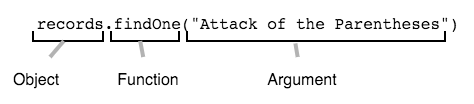
\includegraphics{images/lesson1/oop-js-func.png}
\end{figure}

This object-oriented style \index{object-oriented programming} is very familiar to most JavaScript
programmers and requires little explanation. Next, we'll look at the
perhaps slightly less familiar functional style.\index{functional programming} This style is widely
used in \emph{lodash} and similar libraries.

\begin{figure}[H]
\caption{Functional JavaScript function call}
\centering
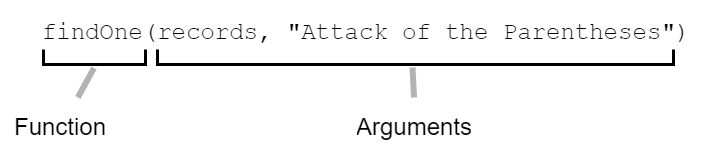
\includegraphics{images/lesson1/func-js-func.png}
\end{figure}

Next, let's look at a ClojureScript version of the same example. Notice
that there are the same number of parentheses in the ClojureScript
version as there were in the JavaScript versions. In fact, the only
differences from the functional JavaScript code is that the left
parenthesis is moved to the left and there is no comma between
arguments.

\begin{figure}[H]
\caption{ClojureScript function call}
\centering
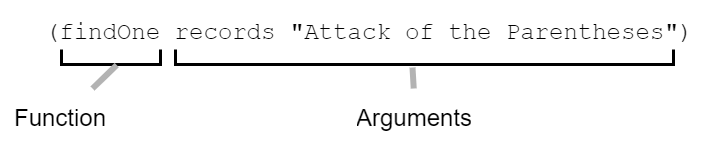
\includegraphics{images/lesson1/cljs-func.png}
\end{figure}

While this is a trivial example, it should be enough to see that
ClojureScript should not be intimidating - different, yes, but not
frightening. As we will see over the coming lessons, we need to adjust
our eyes to read ClojureScript, but the process is not that different
from learning a new library or programming technique.

\subsection{Quick Review}

\begin{itemize}
\tightlist
\item
  Does ClojureScript or JavaScript come with a more extensive standard
  library?
\item
  Does ClojureScript encourage an object-oriented style ot a functional
  style like \emph{lodash} and \emph{ramda}?
\end{itemize}

\section{ClojureScript's Sweet Spots}

While ClojureScript is a general-purpose programming language, it is not
the best tool for every job. If we just want to animate one or two
elements on a webpage or implement an analytics snippet, ClojureScript
is probably overkill (in fact, even jQuery\index{jquery} may be overkill for such
simple examples). How are we to decide, then, when to use ClojureScript
and when to stick with JavaScript? In order decide whether to use
ClojureScript on a project, we should have an idea of the types of
projects in which it excels.

\subsection{Writing Single-Page Applications}

Clojure started out as a general-purpose application programming
language for the JVM, so ClojureScript's heritage is based in
application programming. Indeed we see that the constructs that make
ClojureScript so valuable are precisely those that are necessary for
application-type programs. Specifically, ClojureScript addresses the
JavaScript's issues that start as minor annoyances and escalate to major
issues as an application grows. Anyone who has maintained a large
JavaScript application knows how difficult it is to address strategic
architecture, module loading, cross-browser compatibility, library
selection, tooling, and a whole host of other issues simultaneously.\index{scaling issues}

The problem with JavaScript is that each of these issues must be
addressed separately, but your choice for solving one issue may affect
others.\index{tooling!javascript} For instance, the module system that we use is a separate
concern from our build tool, which in turn is separate from our testing
framework. However, we need to make sure that our build tool supports
our testing framework, and both support our module system or can be
easily integrated with it. Suddenly, the awesome app that we were
planning to write gets stifled by the fact that we just spent 3 days
trying to get the build set up. I can tell you that scenarios like this
are commonplace, since I have experienced a number of them personally.

Paradoxically, ClojureScript makes things easier by taking away choices.
The module system is built in to the language. There is a built-in test
framework. Most libraries provide an API that works on common data
structures in a functional style, so they are simple to integrate.
Additionally, the Google Closure Library\index{Google Closure Library} that is built in will cover
most common concerns such as handling dates, DOM manipulation, HTML5
history, graphics, and ajax. While building a ClojureScript application
is not nearly the adventure that building a JavaScript one is, it is
certainly more productive.

\subsection{Optimizing UIs}

We have alluded to the fact that ClojureScript's immutable data
structures make some interesting UI optimizations possible, but we have
not gone into detail as to how that works. It is really the combination
of React's virtual DOM\index{virtual DOM} concept and ClojureScript's immutable data
structures that make such optimizations possible. Since we know that
ClojureScript's data structures are immutable, we know that any
structure that we create cannot change.\index{immutability} If we have some data structure
backing a UI component, we know that we will not need to re-render the
component as long as it is backed by the same data structure. This
knowledge allows us to create highly optimized UIs.

Consider this: we are writing a contact management app, and we have a
\texttt{ContactList} component that contains \texttt{ContactListItem}
components. These components are all backed by a list of contacts and
should re-render whenever a contact changes. If we were writing the
component using a JavaScript framework, we would either have to put our
data inside special objects that the framework provides so that it can
track changes, use a dirty-checking\index{dirty-checking} mechanism to periodically find what
we need to change, or render everything to an in-memory representation
of the DOM and render any changes to the actual DOM. The ClojureScript
community has adopted the last method, but the story is actually better
in ClojureScript, because we can be selective about which components we
even need to render to the \index{virtual DOM}virtual DOM, saving additional CPU cycles.

\begin{figure}[H]
\caption{Optimizing a UI with immutable data structures}
\centering
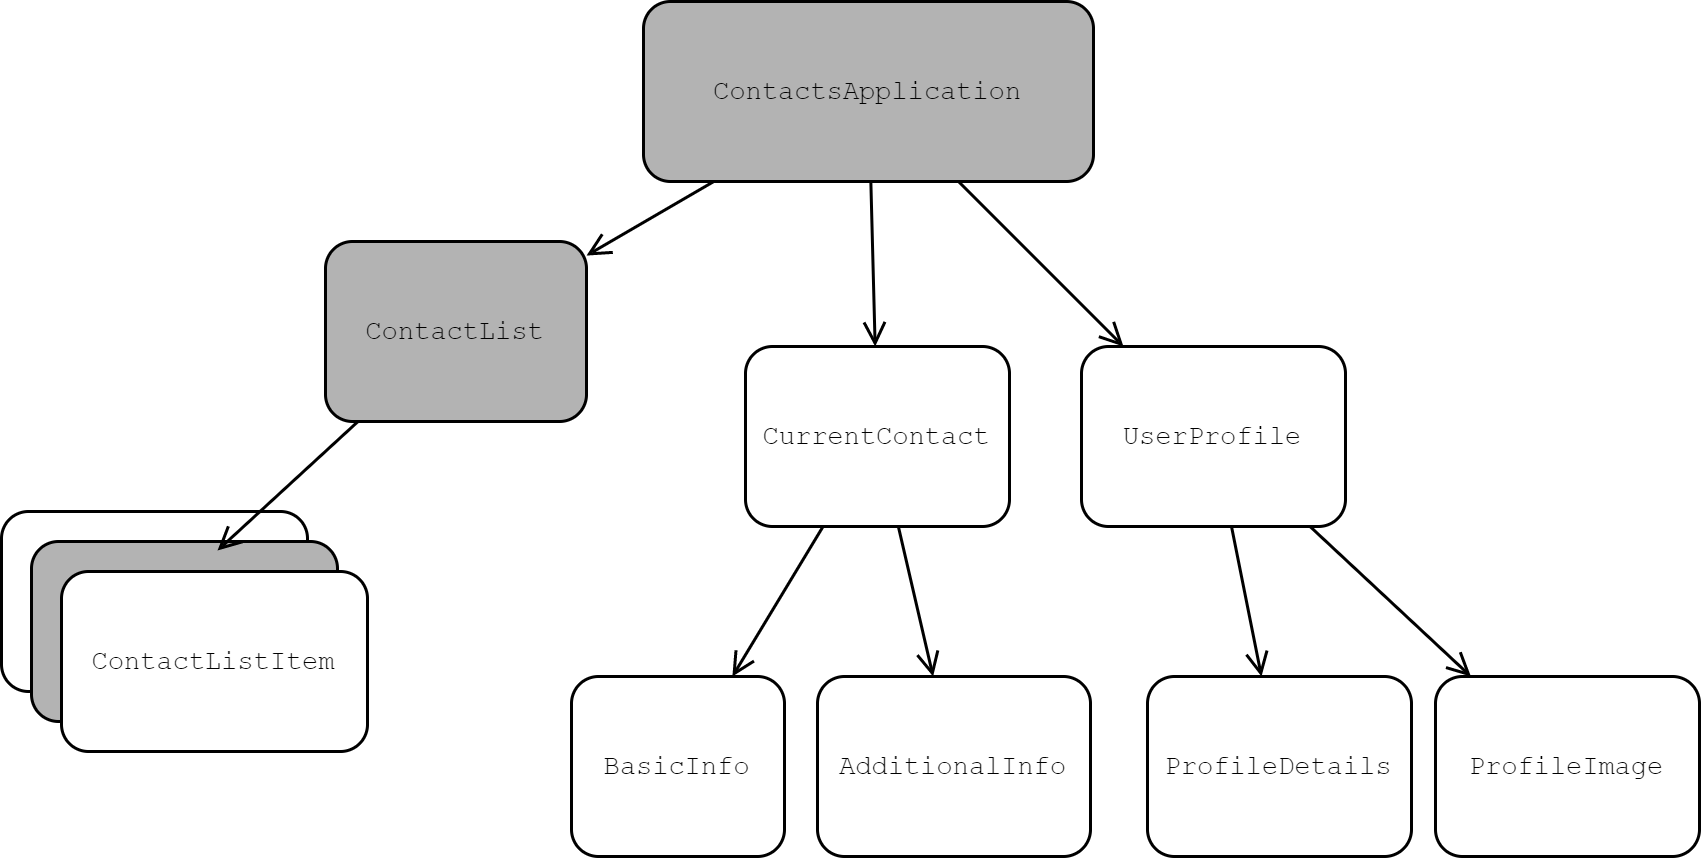
\includegraphics[width=12cm]{images/lesson1/ui-optimization-tree.png}
\end{figure}

In this example, whenever a \texttt{contact} is changed, we replace the
map modeling that contact entirely. When it comes time to render to the
virtual DOM, the \texttt{ContactList} is going to re-render, because the
\texttt{contacts} list is now a new object entirely. Of the
\texttt{ContactListItem} components, only the one that that reflects the
contact we edited is going to re-render. The rest of the
\texttt{ContactListItem}s can quickly see that their underlying data has
not changed, so there is no work to be done. Furthermore, none of the
other portions of the application need to render either. While this
optimization may sound rather minor, we will see later that it can have
a dramatic effect on the performance of an application.

\subsection{Modernizing Async}

JavaScript has now adopted \texttt{async/await}\index{async/await} - which is a first-class
syntax for dealing with promise-like objects - as the preferred way to
achieve asynchronous programming. You will still find raw promises,\index{promises}
callbacks, and generators\index{generators} in some places, but \texttt{async/await} has
become more or less universal.

ClojureScript, on the other hand, has embraced a style of asynchronous
programming called CSP,\index{CSP} or \emph{Communicating Sequential Processes}.
This is the same style of async that has proven so effective in the Go
programming language.\index{Go (programming language)} Using CSP, we do not deal directly with promises
or callbacks. Instead, we think about values and passing them around via
\emph{channels}. For now, you can think of channels as streams or
promises that can deliver more than one value. Additionally, we can
write asynchronous code that looks like synchronous code, tremendously
reducing the cognitive load of writing async code. Performing requests
or getting input sequentially or in parallel are both natural. Some
ClojureScript developers consider async the single most important
advantage that ClojureScript has over JavaScript. We will have to judge
for ourselves when we see it in action later in this book, but know that
it enables a completely new way of thinking about async.

\subsection{Modularizing Design}

In the early days of JavaScript, we probably wrote a single JavaScript
file that we included in every page of a website that covered all of the
scripting that we needed on the site. If the file got too big or
different pages had entirely different requirements, we probably wrote
several JavaScript files and included them on the applicable pages.
Maybe eventually we heard about the ``Module Pattern'' or ``Revealing
Module Pattern'' and separated our code into narrowly focused modules
with one file per module. Now we had to worry about loading every file
in the correct order on the page so that we would not try to reference a
module that did not yet exist. At this point, we probably heard talk of
module loaders that could asynchronously load only the modules we needed
and figure out the correct order to load them in - they could even
concatenate all of our modules into a single file for deployment. The
problem was that there were once again several competing standards for
module loading - AMD, CommonJS, and ES2015.\index{module loading} Even today, finding the
right tooling to integrate modules into our process can be painful, and
every team needs at least one Webpack expert who is aware of the gotchas
of bundling code for deployment.

ClojureScript, on the other hand, has the advantage of being a compiled
language and can provide its own module system with no additional
complexity. ClojureScript uses \emph{namespaces},\index{namespaces} which are named
collections of functions and data, to organize code. Loading order,
preventing circular dependencies, and compiling to a single asset for
production are all part of the standard compiler toolchain. As an added
benefit, the ClojureScript compiler outputs Google Closure modules,
which it then passes off to the Google Closure compiler\index{Google Closure compiler} for additional
optimization, including elimination of dead code paths. Having a good
module system at the language level tremendously simplifies the setup
process of any new project.

\subsection{Quick Review}

\begin{itemize}
\tightlist
\item
  Which of the following projects would be a good fit for ClojureScript?

  \begin{itemize}
  \tightlist
  \item
    single-page app such as a dashboard for a CMS
  \item
    adding animations to a static page
  \item
    web-based game with complex asynchronous user interactions
  \item
    CPU-intensive number-crunching simulations
  \end{itemize}
\item
  Does ClojureScript use the same module systems as JavaScript
  (CommonJS, and ES2015)?
\end{itemize}

\section{ClojureScript 101}

Now that we have seen some of the advantages that ClojureScript can
bring to front-end web development, let's take a step back and survey
ClojureScript's distinct features. As with any technology that promises
to bring significant improvement to the way we code, there will be new
concepts. And as with any new concept, the first step towards mastery is
familiarity. Let's get ready to explore what makes ClojureScript tick.

\subsection{A Compile-to-JavaScript Language}

In 2008, if we were to do any client-side web programming, the only
viable option was JavaScript. Over the next few years, languages that
compiled to JavaScript started to appear. These languages either cleaned
up JavaScript's cruft or added some features that were not present in
JavaScript itself. Some of these languages were modest in their
approach, retaining much of the feel of JavaScript. Others were radical
departures from JavaScript that fell into the category of research
languages. ClojureScript made significant improvements to JavaScript
while sustaining the community support required of a language intended
for professional use. \index{compile-to-JavaScript}

In addition to the other languages that compile to JavaScript, we must
consider the fact that many of us are compiling~newer versions of
JavaScript to older versions so that we can take advantage of language
features that make JavaScript more productive and enjoyable before they
are supported by the major browsers. Starting with the ES2015\index{ES2015} standard,
JavaScript has accumulated many of the best ideas from more recent
programming languages, but since new features are always introduced
quicker than browsers can adopt them, we are perpetually at least a year
away from using ``Modern JavaScript'', and we must unfortunately treat
JavaScript itself as a compile-to-js language! In many fields, this sort
of complexity would be considered insanity, but in web development, this
is the status quo. In contrast to the constant flux of JavaScript,
ClojureScript has remained remarkably stable as a language, with much of
the innovation happening in libraries rather than the language itself.

As with any compile-to-js language, the fact that ClojureScript exists
is a statement that JavaScript is not sufficient. CoffeeScript\index{CoffeeScript} addressed
JavaScript's verbose and inconsistent syntax (it was written in just
over a week, after all). TypeScript\index{TypeScript}, Dart\index{Dart}, and PureScript\index{PureScript} address it's
lack of a type system, enabling developers to better reason about their
code. JavaScript itself addresses the age of the language, bringing more
modern features while maintaining some semblance to previous versions
and providing an easy path to migrate old JavaScript applications.
ClojureScript brings a simpler syntax, an arsenal of data structures
that rule out a whole class of bugs, a better paradigm for asynchronous
programming, and excellent integration with one of the most popular UI
frameworks (React). In short, ClojureScript attempts to be a better
general-purpose front-end language than JavaScript; and the larger the
application, the more its benefits will be evident.

\subsection{A Simple Language}

JavaScript is a chameleon language. Not only is it possible to write
code in imperative, object-oriented, or functional style; it is possible
to mix all of these styles in the same codebase. Even if we consider a
task as simple as iterating over an array, there are quite a few methods
to accomplish this, all of them fairly idiomatic in JavaScript. If we
are most comfortable with the imperative style, we could use a
\texttt{for} loop and manually access each element of the array. On the
other hand, we could use the \texttt{Array.prototype.forEach()} function
(provided we do not have to worry about supporting old browsers).
Finally, if we were already using \emph{lodash} on a project, we could
use one of its helper functions. Each of these methods are demonstrated
below, and they should look familiar to most JavaScript programmers.

\begin{lstlisting}[language=JavaScript, caption={Iterating over an array in JavaScript}]
const numbers = [4, 8, 15, 16, 23, 42];

for (let num of numbers) {                                  %\circled{1}%
  console.log(`The number is ${num}`);
}

numbers.forEach(                                            %\circled{2}%
  (num) => console.log(`The number is ${num}`)
);

const printNum = (num) => {                                 %\circled{3}%
  console.log(`The number is ${num}`);
};
_.each(numbers, printNum);
\end{lstlisting}

\begin{enumerate}[label=\protect\circled{\arabic*}]
\item Imperative
\item Object-oriented
\item Functional
\end{enumerate}

Perhaps more problematic than allowing several styles of programming to
coexist in the same codebase is JavaScript's ``bad parts'' - the quirks
that are the subject of so many technical interview questions. When a
developer first learns JavaScript, there are a number of pitfalls that
she must learn to avoid. Somehow, we have learned to live with all of
the additional complexity laid upon us by JavaScript because we have not
had the luxury of choosing a simpler language. Consider this partial
list of some of JavaScripts quirks and think whether we would be better
off adopting a language without so many gotchas:

\begin{itemize}
\tightlist
\item
  variable hoisting
\item
  several ways to set \texttt{this}
\item
  \texttt{==} vs \texttt{===}
\item
  the \texttt{void} operator
\item
  \texttt{\textquotesingle{}ba\textquotesingle{}\ +\ +\ \textquotesingle{}n\textquotesingle{}\ +\ \textquotesingle{}a\textquotesingle{}\ +\ \textquotesingle{}s\textquotesingle{}}
\item
  What does \texttt{xs.push(x)} return? What about
  \texttt{xs.concat({[}x{]})}?
\end{itemize}

When we consider all of JavaScript's complexity, we can see that we must
code very cautiously or risk being bitten by one of these quirks. For
some simple applications, we may be able to live with this, but as our
codebases grow, the value of a simpler language becomes more and more
apparent. Maintaining a consistent codebase without loads of unnecessary
complexity takes a great deal of skill and discipline. While there are a
lot of expert JavaScript developers out there who do have the requisite
skill and discipline, it does not change the fact that it is
\textbf{hard} to write good JavaScript at the application level.
Thankfully, ClojureScript is a simpler option - admittedly with a
learning curve - but it is generally the things with a steeper learning
curve that ultimately prove the most valuable.

Whereas we have seen that JavaScript promotes a wide variety of
programming styles, ClojureScript is opinionated and is designed to make
the functional style of programming easy. In fact, we will see that
idiomatic ClojureScript looks a great deal like JavaScript written in
the functional style, but with less ceremony. Below is an example of how
you could iterate over a vector, which is similar to a JavaScript array.

\begin{lstlisting}[language=Clojure, caption={Iterating over a vector in ClojureScript}]
(def numbers [4, 8, 15, 16, 23, 42])

(doseq [n numbers]
  (println "The number is" n))
\end{lstlisting}

Like the JavaScript code, this defines a sequence of numbers then logs a
statement to the console for each of the numbers. It even looks pretty
similar to the object-oriented version with the exception that
\texttt{doseq} is not attached to a particular object prototype.\index{object prototype}
However, this - along with some minor variations - is how you can expect
it to look when you need to iterate over a collection in ClojureScript.
Always.

\subsection{A Powerful Language}

One of the spectrums in programming languages is that of how much
functionality to include by default. At one extreme is assembly\index{assembly language}, which
translates directly into CPU instructions and has no ``standard
library'', and at the other end is highly-specialized languages that
include everything necessary to accomplish most any given task in their
problem domain. When it comes to front-end web programming languages,
JavaScript leans more towards the spartan end of the spectrum, and
ClojureScript leans toward the ``batteries included''\index{batteries included} end, providing
higher level tools by default. Between its variety of core data
structures and an extensive collection API, macros that allow for
extension of the language itself, and the entire Google Closure Library\index{Google Closure Library}
available by default, ClojureScript provides more powerful tools for
constructing applications.

\begin{figure}[H]
\caption{Spectrum of programming languages}
\centering
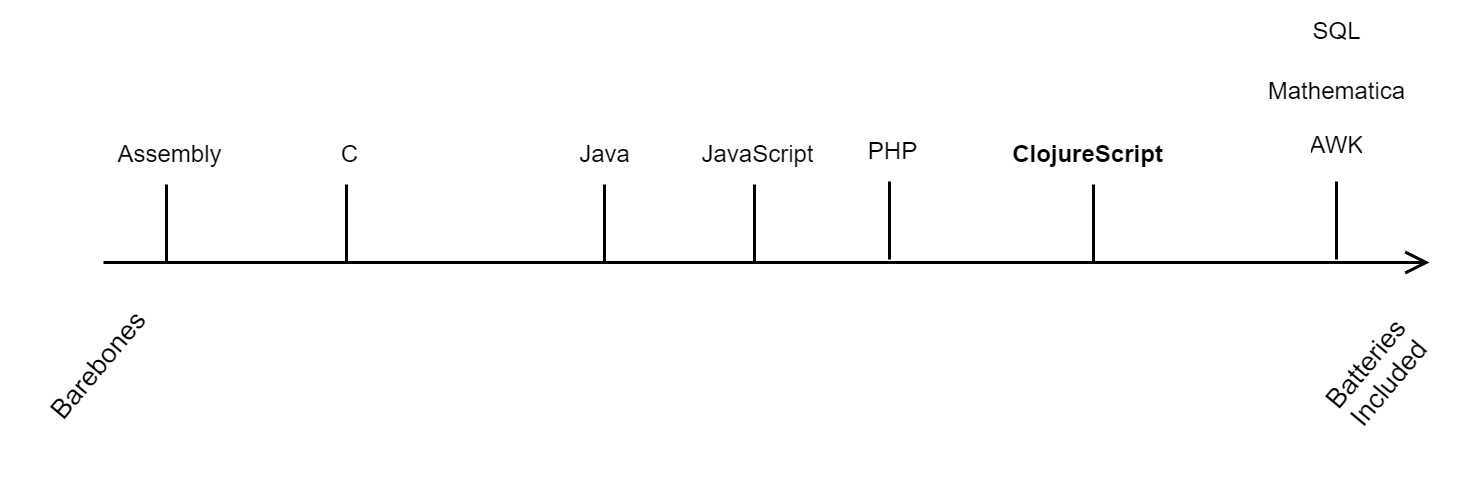
\includegraphics{images/lesson1/lang-spectrum.png}
\end{figure}

The abstractions provided by ClojureScript are higher-level than those
provided by JavaScript, enabling most code to be written more concisely
and descriptively. While JavaScript provides numbers, strings, arrays,
objects, and simple control structures, ClojureScript provides similar
primitives as well as keywords, lists, vectors, sets, maps, protocols,
records, and multimethods. Don't worry if you have no idea what any of
these things are - after all, that is what this book is all about! While
the additional tools mean that there are more things to learn, it also
means that there are fewer occasions to learn a new library or write our
own data structures and generic algorithms.

\subsection{A Functional Language}

Love it or hate it, ClojureScript embraces the concept of functional
programming. If ``functional programming''\index{functional programming} sounds like an intimidating,
academic topic, do not fear - we'll see that most of the functional
programming concepts should be at least somewhat familiar for those of
us who work with JavaScript on a regular basis. This should not be
surprising, since JavaScript was heavily influenced by Scheme\index{Scheme} (a
functional Lisp, just like ClojureScript). Functional programming is one
of the three main styles of programming supported by JavaScript, with an
emphasis on using functions in the mathematical sense of a mapping of
some input value to some output value.

\begin{figure}[H]
\caption{Comparison of JavaScript programming paradigms}
\begin{longtable}[]{@{}lll@{}}
\toprule
\begin{minipage}[b]{0.07\columnwidth}\raggedright
Paradigm\strut
\end{minipage} & \begin{minipage}[b]{0.55\columnwidth}\raggedright
Description\strut
\end{minipage} & \begin{minipage}[b]{0.30\columnwidth}\raggedright
Key Concepts\strut
\end{minipage}\tabularnewline
\midrule
\endhead
\begin{minipage}[t]{0.12\columnwidth}\raggedright
Imperative\strut
\end{minipage} & \begin{minipage}[t]{0.50\columnwidth}\raggedright
Describes a program as a sequence of statements that may modify the
program state, receive input, or produce output.\strut
\end{minipage} & \begin{minipage}[t]{0.30\columnwidth}\raggedright
Variables, loops, assignment, statements, subroutines\strut
\end{minipage}\tabularnewline
\begin{minipage}[t]{0.12\columnwidth}\raggedright
Object-Oriented\strut
\end{minipage} & \begin{minipage}[t]{0.50\columnwidth}\raggedright
Models the real world in terms of objects, their behaviors, and their
interactions with each other.\strut
\end{minipage} & \begin{minipage}[t]{0.30\columnwidth}\raggedright
Objects, classes or prototypes, methods, messages, object graphs\strut
\end{minipage}\tabularnewline
\begin{minipage}[t]{0.12\columnwidth}\raggedright
Functional\strut
\end{minipage} & \begin{minipage}[t]{0.50\columnwidth}\raggedright
Describes a program as a transformation of some input value to some
output value using functions that can be composed.\strut
\end{minipage} & \begin{minipage}[t]{0.30\columnwidth}\raggedright
Pure functions, immutable values, higher-order functions\strut
\end{minipage}\tabularnewline
\bottomrule
\end{longtable}
\end{figure}

While functional programming in JavaScript is gaining momentum, the
majority of code that we are likely to find is either imperative or
object-oriented. Without getting too far into the nitty-gritty of
functional programming at this point, we can say that ClojureScript
focuses on building programs by assembling small functions together that
take some data and return some new data without modifying the arguments
that were passed in or any global state.\index{global state}

One key feature of writing functions this way is that when you call a
function with the same arguments, you always get the same result. While
this may seem like an unimportant property for a function, it makes
testing and debugging much easier. If most of a program is written as
pure functions, tests can be written without any set-up. Contrast this
with the typical way that object-oriented systems are tested: a number
of objects must be constructed and put in to just the right state before
every test, or the test will not run correctly.

\subsection{Quick Review}

\begin{itemize}
\tightlist
\item
  Is the ClojureScript language stable? Why or why not?
\item
  List at least 3 ways in which ClojureScript improves upon JavaScript
\item
  What is the difference between \emph{simplicity} and
  \emph{familiarity}? What are some aspects of JavaScript that are not
  simple?
\item
  Does ClojureScript or JavaScript operate at a higher level of
  abstraction?
\item
  Of the 3 styles of programming that are common in JavaScript
  (imperative, object-oriented, and functional), which is encouraged by
  ClojureScript?
\end{itemize}

\section{Summary}

ClojureScript is an incredible useful language, particularly for
front-end web development. It shares many of JavaScript's functional
programming concepts, but it is both a simpler and more productive
language. ClojureScript may appear foreign with all its parentheses, but
under the parenthesis-packed surface, it shares much in common with
JavaScript. We should now understand:

\begin{itemize}
\tightlist
\item
  What ClojureScript is and what sets it apart from JavaScript
\item
  What types of apps are the best fit for ClojureScript
\end{itemize}

%% Lesson 2

\chapter{ClojureScript in the JavaScript Ecosystem}

Now that we have a good idea of what ClojureScript is and how to use it,
we will continue to pull back the curtain to get a clearer picture of
how this curious language fits into its environment - the JavaScript
ecosystem. While the language is quite different from JavaScript, it
maintains a symbiotic relationship to its JavaScript host. JavaScript
needs ClojureScript, and ClojureScript needs JavaScript. Let's explore
this interesting symbiosis.

\begin{center}\rule{0.5\linewidth}{0.5pt}\end{center}

\textbf{In this lesson:}

\begin{itemize}
\tightlist
\item
  What problems in JavaScript does ClojureScript try to solve?
\item
  How using a compiled language helps in application development
\item
  Why is JavaScript an ideal platform for ClojureScript?
\end{itemize}

\begin{center}\rule{0.5\linewidth}{0.5pt}\end{center}

\section{Why JavaScript Needs Clojure}

Having seen ClojureScript's sweet spots, it should be apparent that
there are some gains that it promises. Still, can we get a similar
advantage from JavaScript itself without having to learn a new language?
Also, does ClojureScript really give us that much additional leverage in
our daily development tasks? ClojureScript may not be the best tool for
trivial tasks, but for anything more complex, JavaScript does in fact
\emph{need} a language like Clojure to enable more productive and
enjoyable development.

\begin{notice}[title={Clojure(Script)}]
You may have noticed several times where I have used the terms
``Clojure'' and ``ClojureScript'' interchangeably.\index{Clojure} Clojure as a language
has implementations that compile to both Java bytecode and to
JavaScript. Some of the potential confusion comes from the fact that
``Clojure'' refers to both the language and its Java implementation. I
will follow the general pattern of the Clojure community of using the
two terms interchangeably when talking about the language itself and
using ``ClojureScript'' when discussing the ecosystem or language
features that are specific to ClojureScript.
\end{notice}

\subsection{Higher Level Language}

ClojureScript operates with higher-level constructs than JavaScript. In
JavaScript, we work largely with variables, loops, conditional branching
structures, objects and arrays. In ClojureScript, we work with
expressions, collections, sequences, and transformations. The journey
from lower-level concepts to higher-level ones is the way that we gain
productivity.

\begin{figure}[H]
\caption{Features defining each level of abstraction}
\centering
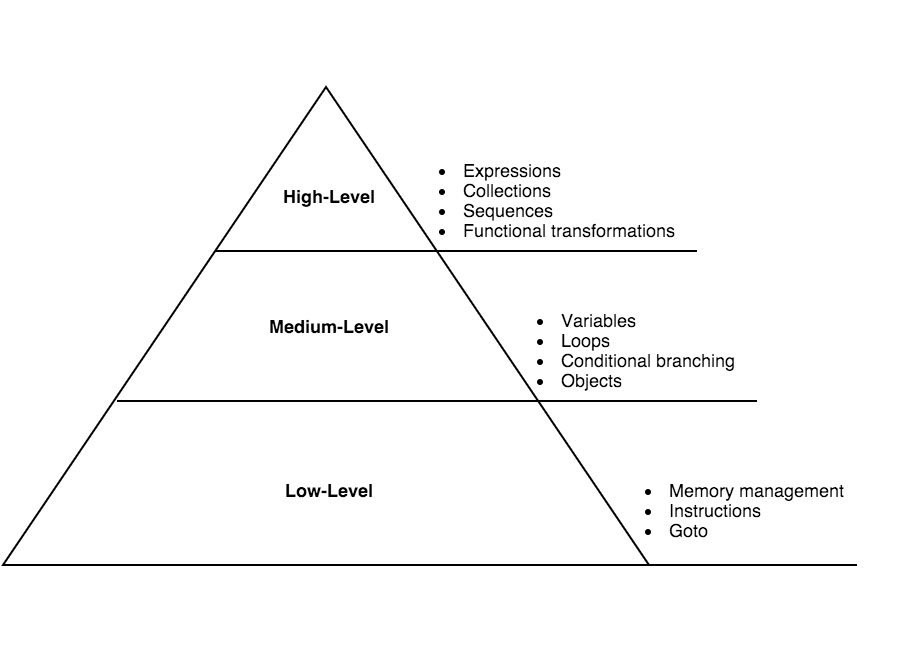
\includegraphics{lesson2/language-hierarchy.png}
\end{figure}

When we work at a higher level, a couple of interesting things happen.
First, it takes less code to accomplish a given task, which helps with
both initial development and debugging/maintenance. Second, it causes
the structure of the code more closely resemble the problem domain,
making it clearer for us to understand when we come back to it. Third,
it frees us to think more about the problems of the domain rather than
technical implementation issues. All of these factors can enable huge
productivity boosts, both in the initial development and maintenance
phases of an application.

When we write less code to accomplish a given task, there are a couple
of benefits. First, it almost goes without saying that it is quicker to
write a little code than it is a lot of code. Even though more time is
usually spent designing and planning code than actually writing it, we
do not want to be hampered by how many keystrokes it takes to turn our
ideas into code. Second, fewer lines of code means fewer bugs. The
developer who would rather spend her time fixing bugs than writing new
features is either a rarity or nonexistent. The terseness of a
high-level language like ClojureScript means that there are fewer places
for bugs to hide, and in turn, we can spend more time making forward
progress.

\subsection{Less Boilerplate}

I cannot count the times that I have had a simple task that I wanted to
accomplish with JavaScript - say, performing a deep clone of an object -
but had to do a Google search to remember how to do it either using
vanilla JavaScript or the libraries that I had available. Usually, I
would end up on some StackOverflow thread that I had already visited
numerous times and copying and pasting the example into yet another
``utils'' file in yet another project. Libraries such as \emph{lodash}\index{Lodash}
(and \emph{jQuery}\index{jQuery} for you history buffs out there) help compensate for
JavaScript's lack of common utilities, but they do not solve the problem
that one must look beyond the language itself to get the functionality
of a robust standard library.\index{JavaScript!standard library}

The problem of needing to pull in third-party libraries\index{third-party libraries} for most tasks
is uniquely problematic for the browser because every additional library
adds time to the page load. Compound this issue with the fact that most
web apps at least need to consider mobile clients\index{mobile clients} with slow networks.
When every byte counts, as it does on the web, we are continually faced
with the question of whether to include another library for limited
utility or write the functions that we need from scratch.

Finally, JavaScript developers must continually face the reality of
browser compatibility\index{browser compatibility} issues. The available options are to target the
lowest common denominator of the browser that you would like to support
(and miss out on the language features that improve developer
productivity), pull in libraries (and add substantial page size), or
implement browser-detection and write the browser-specific portions from
scratch (and face the additional complexity that comes with browser
hacks). The choices do not sound very attractive, and we should not have
to make a trade-off between developer productivity, performance, and
complexity. In order to solve the browser compatibility problem without
sacrificing any of these things, we need to look outside JavaScript
itself.

ClojureScript, on the other hand, has a rich set of data structures and
functions for working with collections, strings, math, state management,
JavaScript interoperability, and more. Additionally, ClojureScript is
built on top of Google's Closure (with an ``s'', not a ``j'') library\index{Google Closure Library},
putting the same tools that power applications like Gmail and Google
Docs at your fingertips. With so many tools at our disposal, we'll see
that the amount of utility code that we need to write is minimal.
Finally, ClojureScript compiles down to a widely-supported subset of
JavaScript, making browser compatibility much less of an issue.
ClojureScript takes the focus off the ``plumbing'', allowing us to focus
more on the interesting problems of the domain in which we are working.

\subsection{Immutable Data by Default}

We have already looked at immutable data as one of the fundamental
concepts of functional programming. While much of the JavaScript
community is starting to recognize the value of immutable data, working
with immutable data in JavaScript is still not native and can feel
somewhat cumbersome. Libraries like \emph{immer}\index{immer} and \emph{Immutable.js}\index{Immutable.js}
allow us to get the benefits of immutable data from JavaScript, but once
again, the language currently has no native support.

In ClojureScript, however, the situation is reversed. All of the default
data structures are immutable, and we have to go out of our way to work
with mutable objects. This is one area where ClojureScript is very
opinionated, but the style of programming that it promotes is one that
will lead to fewer bugs and - as we have already seen - optimized user
interfaces. Once we have become accustomed to using ClojureScript's data
structures, returning to mutable objects and arrays will feel unusual -
even dangerous.

\subsection{Compiler Optimized}

One advantage that a compiled language has is that it can implement
optimizations in the JavaScript code that it produces. It is rare for a
high-level language to match either the speed, resource usage, or
compiled code size of a lower-level language. ClojureScript, however,
can often produce JavaScript that runs as fast as hand-written
JavaScript. Its immutable data structures do usually consume more memory
and are slower than raw objects and arrays, but the UI optimizations
afforded by these data structures can make ClojureScript interfaces
\emph{effectively faster} than a corresponding JavaScript interface.

One metric that matters a great deal to JavaScript programmers is code
size. When working in a server-side environment, the code size is
usually not a concern - the code is read from disk and immediately read
into memory. However, with front-end JavaScript applications, the code
usually must be read over the internet, potentially over a low-bandwidth
mobile network. In this situation, every byte counts, and we are used to
laboring over our code and trying to make it as small as possible, even
at the cost of clarity. Minification\index{minification} helps tremendously, but we still
must be mindful about including more libraries. Often, the benefit added
by a library is offset by the kilobytes that it adds to page load time.

One of the most interesting features of the ClojureScript compiler is
that it produces Google Closure modules, and it then makes use of the
Closure Compiler to optimize the JavaScript. Since the ClojureScript
compiler guarantees that the JavaScript it produces is valid Google
Closure modules, we can safely make use of the Closure Compiler's most
aggressive optimizations when preparing production assets. In addition
to the typical removal of whitespace and renaming variables, the Closure
Compiler will analyze an entire codebase and remove any code paths that
can never be called. Effectively, this means that we can pull in a large
library, and if we use only a couple of functions from this library,
only those functions and the functions they call are included in our
codebase. In an environment where code size is so critical, this is
clearly a significant advantage.

\subsection{Quick Review}

\begin{itemize}
\tightlist
\item
  Can you think of any pieces of code that you find yourself writing for
  almost every JavaScript project? Would any of these be solved by a
  more complete standard library?
\item
  What is the advantage of working in a language that compiles to
  JavaScript Can you think of any disadvantages?
\end{itemize}

\section{Why Clojure needs JavaScript}

As useful as the Clojure language is, it needs JavaScript. The most
significant things that JavaScript enable for the Clojure language are
client-side web development, the rich ecosystem of libraries and
technologies, and a much lighter-weight platform with a smaller
footprint than the Java Virtual Machine.\index{Java Virtual Machine} That said, ClojureScript
compiles to JavaScript, so it runs where JavaScript does, including the
client, server, desktop, and Internet of Things (IoT) devices.

\subsection{Client-Side Development}

Clojure was originally a server-side language. It was certainly possible
to write desktop GUIs using Swing or another Java UI toolkit, but the
vast majority of Clojure was written for the server. Clojure is
excellent as a server-side programming language, but as we have
discussed, it brings some significant advantages to UI development as
well. With the advent of ClojureScript, Clojure is now a general-purpose
language that can be used for almost any application - on the server or
client. As Rich Hickey stated when he announced ClojureScript, ``Clojure
\emph{rocks}, and JavaScript \emph{reaches}.''

Additionally, with technologies like Electron\index{Electron} and NW.js, we have the
option of writing desktop applications in JavaScript as well; and since
ClojureScript compiles to JavaScript, we can take advantage of the same
technologies to write desktop applications in ClojureScript as well.
While Clojure itself enables developers to write Java GUI applications,
many developers prefer the lighter- weight style afforded by these
JavaScript UI technologies.

\begin{notice}[title={ClojureScript on the Desktop}]
The developers of the LightTable\index{Light Table} editor - one of the most popular
editors supporting the Clojure language - opted to build their UI using
ClojureScript and deploy inside Electron. This enabled them to build an
incredibly flexible, customizable UI without the complexity of a
traditional desktop UI.
\end{notice}

Finally, there are a few technologies that allow JavaScript applications
to run as mobile apps. React Native is gaining a lot of traction in this
area, making it an excellent choice for ClojureScript, since most
ClojureScript UIs are built on React as a platform. While this area of
JavaScript mobile native apps is relatively new territory, it is showing
a lot of promise. The next generation of mobile apps may be
predominantly JavaScript apps, which means that ClojureScript will be a
first-class citizen for mobile clients as well.

\subsection{JavaScript Ecosystem}

JavaScript is more than just a language - it is a community that has
opinions on best practices, libraries, tooling, and development process.
It is in this community that ClojureScript lives. While we as
ClojureScript developers benefit from the vast number of JavaScript
libraries available, the more significant benefit provided by JavaScript
is its community. We can learn from the collective experience of the
community what is the good, the bad, and the ugly of front-end
development. The relationship between JavaScript and Clojure is truly
symbiotic, with both communities benefitting from the ideas and insights
of the other.

While we have seen that ClojureScript is a very practical and useful
language, let's face it - it is easy for a functional programming
language to lose touch with the concerns of working programmers.
Theoretical languages are useful, and most useful programming language
features started out as research projects, but theoretical purity is not
our top concern when writing web apps. Get-it-done-ability is a much
higher priority, and from its inception, JavaScript has been about
getting things done as straightforwardly as possible. Being a citizen of
the JavaScript community helps ClojureScript stay focused on pragmatic
concerns that help us build better web applications.

\subsection{Smaller Footprint}

The JVM\index{Java Virtual Machine} is an excellent platform for developing high-performance
cross-platform applications. It is not so excellent when it comes to
running in resource-constrained environments or scripting. While the
slogan ``Write once, run anywhere'' was used by Sun Microsystems to
promote Java, it is ironically JavaScript that has become a
``universal'' runtime. From the browser to the server to the Raspberry
Pi and embedded devices, JavaScript will run just about anywhere.
Running Java on something like a Raspberry Pi\index{Raspberry Pi}, on the other hand, is a
practical impossibility. ClojureScript is a great option for writing
applications where Java is too much bloat. Its ability to run on almost
any device is another aspect of JavaScript's ``reach'' that we can take
advantage of from ClojureScript.

Scripting is another area where Java is fairly weak. Whether as a
scripting language embedded in a larger application or as a system shell
scripting language, Java is too large and complex, and the startup time
of the JVM makes it impractical for short-lived programs like simple
scripts. JavaScript is a great scripting language. Node.js allows us to
write system scripts as well as web servers.\index{Node.js}

\subsection{Quick Review}

\begin{itemize}
\tightlist
\item
  What is the most common platform for ClojureScript - web, desktop,
  mobile, or IoT devices? Can it be used outside this platform?
\item
  How well does ClojureScript interoperate with existing JavaScript
  tools and libraries?
\end{itemize}

\section{Summary}

In this lesson, we have explored the relationship of ClojureScript to
its host, JavaScript. We have learned:

\begin{itemize}
\tightlist
\item
  How ClojureScript improves on JavaScript's development experience
\item
  How JavaScript's lightweight and ubiquitous runtime allows us to write
  ClojureScript for practically any platform.
\item
  Why client-side web development is a great fit for ClojureScript.
\end{itemize}

Now that we have a good understanding of both what ClojureScript is and
how it is related to the JavaScript platform, we are ready to see the
language in action. In the next section, we will work through the
process of writing a ClojureScript application, learning the common
tools and practices as we go.

%% Lesson 3

\chapter{Building Blocks}

With an understanding of what ClojureScript is and why it matters, we
will begin our journey with an overview of the basics of the language.
One of the biggest hurdles in learning an unfamiliar language is
understanding the syntax. While there is a great deal of crossover
between languages at the conceptual level, the way that those concepts
are expressed can be quite different. Over the next two lessons, we will
hone in on the foundational skill of reading ClojureScript code. Even
though the syntax is so simple compared to JavaScript, it looks very
unusual to most programmers who have cut their teeth on C-like languages
(including JavaScript). The skill of reading ClojureScript will go a
long way towards being able to read the longer code samples in the
coming lessons with ease.

\begin{center}\rule{0.5\linewidth}{0.5pt}\end{center}

\textbf{In this lesson:}

\begin{itemize}
\tightlist
\item
  Learn the basics of ClojureScript's syntax
\item
  Understand the purpose of all the parentheses
\item
  Survey the core data types that are built in to the language
\end{itemize}

\begin{center}\rule{0.5\linewidth}{0.5pt}\end{center}

First, in this lesson, we will survey the most common syntactic elements
of the language, then in the next lesson we will take a look at how
ClojureScript code is actually evaluated. Understanding the evaluation
model will help us both understand the code we read and write code that
does exactly what we expect it to. ClojureScript is a very small
language - much smaller than JavaScript - so it is very simple to
understand. Despite the foreign syntax, we can reach a point of
familiarity surprisingly quickly due to the relatively few syntactic
elements of the language.

\section{Parens, Parens Everywhere!}

As we have seen in the examples of the previous lessons, ClojureScript
code is replete with parentheses. For many, this single aspect of the
language is what makes it seem intimidating. Parentheses are the primary
symbols used for delineating one piece of code from another. Consider
that JavaScript and other languages in the C family use both parentheses
and curly brackets - parentheses to indicate parameters to a function
and to specify the order of operations and curly brackets to set apart
blocks of related statements. Once we get over the initial ``paren
shock'', ClojureScript begins to look simple, even elegant.

\subsection{Expressions and Function Evaluation}

Parentheses are used in ClojureScript to indicate expressions to be
evaluated. We will look much deeper into these so called
\texttt{s-expressions}\index{s-expressions} in the next lesson, but they are so critical that
we must at least mention them here. At a high level, every ClojureScript
program has basically the following form:

\begin{lstlisting}[language=Clojure, caption={ClojureScript function expression}]
(some-function arg1 arg2 ...)
\end{lstlisting}

Whenever there is an open parenthesis, the next thing that the compiler
expects is something that can be called - usually a function. Everything
else until the next closing parenthesis is expected to be an argument.

\begin{figure}[H]
\caption{A Simple Expression}
\centering
\includegraphics{lesson3/simple-expression.png}
\end{figure}

If we were to write the same general structure in JavaScript, it would
look something like the following:

\begin{lstlisting}[language=JavaScript, caption={JavaScript function expression}]
someFunction(arg1, arg2, ...);
\end{lstlisting}

Both the ClojureScript and JavaScript code indicate that there is some
function that should be called with some number or arguments. While the
JavaScript code indicates a function call by putting the name of the
function first, followed by some arguments enclosed in parentheses,
ClojureScript indicates the same thing by enclosing both the function
name and its arguments within a set of parentheses.

\section{Core Data Types}

ClojureScript has all of the primitive data types\index{data types!primitives} that we would expect
from any programming language: numbers, strings, booleans, and the like.
We refer to these simple values as scalars. Additionally, the language
has a variety of useful \emph{collection} types as well - think arrays
and objects from JavaScript. These collections are so frequently used
that there is special syntax for representing them. Before diving into
each of the data types, it bears enumerating a complete list of data
types for reference. The following table lists the types that have a
literal syntactic representation, along with a brief description and an
example of how it is expressed in code.

\subsubsection{ClojureScript Data Literals}

\begin{longtable}[]{@{}lll@{}}
\toprule
\begin{minipage}[b]{0.15\columnwidth}\raggedright
Data Type\strut
\end{minipage} & \begin{minipage}[b]{0.51\columnwidth}\raggedright
Description\strut
\end{minipage} & \begin{minipage}[b]{0.33\columnwidth}\raggedright
Example\strut
\end{minipage}\tabularnewline
\midrule
\endhead
\begin{minipage}[t]{0.07\columnwidth}\raggedright
Number\strut
\end{minipage} & \begin{minipage}[t]{0.51\columnwidth}\raggedright
Integer or floating point numbers\strut
\end{minipage} & \begin{minipage}[t]{0.33\columnwidth}\raggedright
\texttt{17.4}\strut
\end{minipage}\tabularnewline
\begin{minipage}[t]{0.07\columnwidth}\raggedright
String\strut
\end{minipage} & \begin{minipage}[t]{0.51\columnwidth}\raggedright
Textual data\strut
\end{minipage} & \begin{minipage}[t]{0.33\columnwidth}\raggedright
\texttt{"Today\ is\ the\ first\ day..."}\strut
\end{minipage}\tabularnewline
\begin{minipage}[t]{0.07\columnwidth}\raggedright
Character\strut
\end{minipage} & \begin{minipage}[t]{0.51\columnwidth}\raggedright
Textual data\strut
\end{minipage} & \begin{minipage}[t]{0.33\columnwidth}\raggedright
\texttt{\textbackslash{}a}\strut
\end{minipage}\tabularnewline
\begin{minipage}[t]{0.07\columnwidth}\raggedright
Boolean\strut
\end{minipage} & \begin{minipage}[t]{0.51\columnwidth}\raggedright
Logical true/false\strut
\end{minipage} & \begin{minipage}[t]{0.33\columnwidth}\raggedright
\texttt{true}\strut
\end{minipage}\tabularnewline
\begin{minipage}[t]{0.07\columnwidth}\raggedright
Keyword\strut
\end{minipage} & \begin{minipage}[t]{0.51\columnwidth}\raggedright
Lightweight identifiers\strut
\end{minipage} & \begin{minipage}[t]{0.33\columnwidth}\raggedright
\texttt{:role}\strut
\end{minipage}\tabularnewline
\begin{minipage}[t]{0.07\columnwidth}\raggedright
Symbol\strut
\end{minipage} & \begin{minipage}[t]{0.51\columnwidth}\raggedright
Identifiers that are extensively used internal to ClojureScript\strut
\end{minipage} & \begin{minipage}[t]{0.33\columnwidth}\raggedright
\texttt{\textquotesingle{}cljs-is-awesome}\strut
\end{minipage}\tabularnewline
\begin{minipage}[t]{0.07\columnwidth}\raggedright
List\strut
\end{minipage} & \begin{minipage}[t]{0.51\columnwidth}\raggedright
Ordered collection supporting efficient traversal\strut
\end{minipage} & \begin{minipage}[t]{0.33\columnwidth}\raggedright
\texttt{\textquotesingle{}(1\ 3\ 5\ 7\ 9)}\strut
\end{minipage}\tabularnewline
\begin{minipage}[t]{0.07\columnwidth}\raggedright
Vector\strut
\end{minipage} & \begin{minipage}[t]{0.51\columnwidth}\raggedright
Ordered collection supporting efficient access by index\strut
\end{minipage} & \begin{minipage}[t]{0.33\columnwidth}\raggedright
\texttt{{[}0\ 2\ 4\ 6\ 8{]}}\strut
\end{minipage}\tabularnewline
\begin{minipage}[t]{0.07\columnwidth}\raggedright
Map\strut
\end{minipage} & \begin{minipage}[t]{0.51\columnwidth}\raggedright
Unordered collection associating unique keys to values\strut
\end{minipage} & \begin{minipage}[t]{0.33\columnwidth}\raggedright
\texttt{\{:name\ "Kayleigh",\
\ :age\ 29\}}\strut
\end{minipage}\tabularnewline
\begin{minipage}[t]{0.07\columnwidth}\raggedright
Set\strut
\end{minipage} & \begin{minipage}[t]{0.51\columnwidth}\raggedright
Unordered collection of unique values\strut
\end{minipage} & \begin{minipage}[t]{0.33\columnwidth}\raggedright
\texttt{\#\{true\ "ubiquity"\ 9.2\}}\strut
\end{minipage}\tabularnewline
\begin{minipage}[t]{0.07\columnwidth}\raggedright
nil\strut
\end{minipage} & \begin{minipage}[t]{0.51\columnwidth}\raggedright
The empty value\strut
\end{minipage} & \begin{minipage}[t]{0.33\columnwidth}\raggedright
\texttt{nil}\strut
\end{minipage}\tabularnewline
\begin{minipage}[t]{0.07\columnwidth}\raggedright
Object\strut
\end{minipage} & \begin{minipage}[t]{0.51\columnwidth}\raggedright
JavaScript object - used for interop\strut
\end{minipage} & \begin{minipage}[t]{0.33\columnwidth}\raggedright
\texttt{\#js\ \{"isJs"\ true,\ "isImmutable"\ false\}}\strut
\end{minipage}\tabularnewline
\begin{minipage}[t]{0.07\columnwidth}\raggedright
Array\strut
\end{minipage} & \begin{minipage}[t]{0.51\columnwidth}\raggedright
JavaScript array - user for interop\strut
\end{minipage} & \begin{minipage}[t]{0.33\columnwidth}\raggedright
\texttt{\#js\ {[}"Lions"\ "Tigers"\ "Bears"{]}}\strut
\end{minipage}\tabularnewline
\bottomrule
\end{longtable}

We will now look at each data type in turn and see a few examples of its
usage so that we can identify the various elements in any given piece of
ClojureScript code.

\subsection{Numbers}

\index{data types!numbers}ClojureScript uses JavaScript's Number primitive, so it can support
exactly the same integer and floating point numbers that JavaScript
does. Below are examples of the different formats that ClojureScript
recognizes as valid numbers.

\begin{lstlisting}[language=Clojure, caption={Numbers}]
32                                                         %\circled{1}%

012                                                        %\circled{2}%

0xbeef                                                     %\circled{3}%

0.6                                                        %\circled{4}%

1.719493e3                                                 %\circled{5}%

-0.12e-4                                                   %\circled{6}%
\end{lstlisting}

\begin{enumerate}[label=\protect\circled{\arabic*}]
\tightlist
\item  Decimal integer
\item Octal integer starts with a leading zero
\item Hexadecimal integer starts with leading \texttt{0x}
\item Float
\item Float with an exponent
\item Float with a sign and exponent with a sign
\end{enumerate}

\subsection{Strings}

\index{data types!strings}Strings, like numbers, use JavaScript primitives. However,
ClojureScript's string syntax is more restricted than JavaScript's.
Notably, strings \emph{must} be contained in double quotes, since
ClojureScript uses single quotes for other purposes. Double quotes and
other special characters are escaped with a backslash.

\begin{lstlisting}[language=Clojure, caption={Strings}]
"Quick! Brown foxes!"                                        %\circled{1}%

\a                                                           %\circled{2}%

"Column 1\tColumn 2"                                         %\circled{3}%

"foo
bar"                                                         %\circled{4}%
\end{lstlisting}

\begin{enumerate}[label=\protect\circled{\arabic*}]
\tightlist
\item Simple string
\item Single character strings can be represented by the character proceeded by a backslash
\item String with special character
\item Strings can span multiple lines
\end{enumerate}

\subsection{Booleans}

\index{data types!booleans}ClojureScript also uses JavaScript booleans. Since the only possible
options for a boolean are \texttt{true} or \texttt{false}, we will
forego an extended example.

\subsection{Keywords}

\index{data types!keywords}We now encounter a data type that does not have a JavaScript equivalent.
A keyword is represented by a name preceded by a colon. Keywords
evaluate to themselves, and two keywords with the same name are
considered equal. One interesting property of keywords is that they can
be used as a function. When used as a function, the keyword expects a
map as an argument and it will return the value in the map for which it
is the key. When a keyword begins with two colons, the current namespace
will be prepended to the keyword.

\begin{lstlisting}[language=Clojure, caption={Keywords}]
:a-keyword                                                  %\circled{1}%

::namespaced-keyword                                        %\circled{2}%

:explicit-ns/keyword                                        %\circled{3}%

{:name "Bill", :type "admin"}                               %\circled{4}%

(:type user)                                                %\circled{5}%
\end{lstlisting}

\begin{enumerate}[label=\protect\circled{\arabic*}]
\item Imperative
\tightlist
\item Simple keyword
\item With implicit namespace - shorthand for \texttt{:cljs.user/namespaced-keyword}
\item With explicit namespace
\item Used as keys in a map
\item Used as a function to perform a map lookup
\end{enumerate}

\subsection{Symbols}

\index{data types!symbols}Symbols are an interesting data type because they are closely linked to
the Lisp family of programming languages from which ClojureScript is
derived. Symbols are names that usually evaluate to some other object.
We have seen symbols in almost every example without even thinking about
it.

\begin{lstlisting}[language=Clojure, caption={Symbols}]
my-function                                                 %\circled{1}%

first                                                       %\circled{2}%
\end{lstlisting}

\begin{enumerate}[label=\protect\circled{\arabic*}]
\tightlist
\item Symbol referring to a user-defined variable
\item Symbol referring to a built-in function
\end{enumerate}

Of ClojureScript's data types, symbols are probably the most difficult
to comprehend. They have a very meta quality about them, and they do not
directly correspond to another familiar concept. When ClojureScript code is evaluated, it will try to resolve a symbol to the thing that it names. Sometimes, we want to refer to a symbol itself rather than the thing that it names, in which case we can place a single quote in front of the symbol to "quote" it, instructing the ClojureScript reader to not evaluate it.
Since they are not used
very commonly in application code, we will not revisit symbols to the
depth that we will with the other data types.

\subsection{Lists}

\index{data types!lists}Lists are comprised of a number of expressions inside parentheses.
However, remember that s-expressions are also written the same way. For
this reason, we designate a list that should not be evaluated as an
s-expression by placing a quote before it. It is interesting to note
that ClojureScript code is actually made up of lists.

\begin{lstlisting}[language=Clojure, caption={Lists}]
(+ 1 2 3 4)                                                 %\circled{1}%

'(+ 1 2 3 4)                                                %\circled{2}%

'(some data)                                                %\circled{3}%

'()                                                         %\circled{4}%
\end{lstlisting}

\begin{enumerate}[label=\protect\circled{\arabic*}]
\tightlist
\item A list that is interpreted as an expression and evaluated
\item Prevent evaluation of a list by starting it with a single quote
\item Lists can contain any ClojureScript data type
\item An empty list
\end{enumerate}

\subsection{Vectors}

\index{data types!vectors}Vectors are comprised of a number of expressions contained inside square
brackets. When ClojureScript encounters a vector, it will interpret it
as a data structure and will not try to evaluate it as a function call.
They are used in a similar manner to JavaScript arrays and are the most
common data structure in ClojureScript. Vectors are also used to list
the arguments that a function takes.

\begin{lstlisting}[language=Clojure, caption={Vectors}]
[]                                                          %\circled{1}%

["Alice" "Bob" "Carol"]                                     %\circled{2}%

(defn say-hello [name]                                      %\circled{3}%
  (println "Hello," name))
\end{lstlisting}

\begin{enumerate}[label=\protect\circled{\arabic*}]
\tightlist
\item An empty vector
\item A vector used to define a collection of strings
\item A vector used to declare a function's argument list
\end{enumerate}

\subsection{Maps}

\index{data types!maps}Maps are collections similar to a JavaScript object. They associate
unique keys with values and can subsequently be used to lookup values by
key. The syntax for a map is even similar to that of a JavaScript
object, since it consists of a number of key-value pairs inside curly
brackets. Either commas or newlines are often used to separate pairs.
Commas are whitespace in ClojureScript, and we will frequently find them
omitted.

\begin{lstlisting}[language=Clojure, caption={Maps}]
%\circled{1}%
{}                                                          %\circled{1}%

{"product" "Self-Sealing Stem Bolt"                         %\circled{2}%
 "sku" "DS9-SB09"
 "stock" 212}

{:name "Jorge", :age 29}                                    %\circled{3}%
\end{lstlisting}

\begin{enumerate}[label=\protect\circled{\arabic*}]
\tightlist
\item An empty map
\item A map using strings as keys
\item A map using keywords as keys
\end{enumerate}

\subsection{Sets}

\index{data types!sets}Sets are an unordered collection of unique elements. They are often used
when we want to avoid duplicates or need to quickly determine whether an
element is in a collection. Sets are declared with any number of
elements contained inside curly brackets that are prefixed with a pound
sign.


\begin{lstlisting}[language=Clojure, caption={Sets}]
#{}                                                         %\circled{1}%

#{"admin" "editor" "author" "subscriber"}                   %\circled{2}%
\end{lstlisting}

\begin{enumerate}[label=\protect\circled{\arabic*}]
\tightlist
\item An empty set
\item A set with several unique strings
\end{enumerate}

Of the data structures that have their own syntax, sets are probably the
least often used. It is still important to be able to recognize them,
since at first glance they look quite similar to a map.

\subsection{Nil}

\index{data types!nil}Nil is the empty value and is always written as \texttt{nil}. It is the
equivalent of \texttt{null} in JavaScript and acts the same as
\texttt{false} when used as a boolean.

The JavaScript interop forms will be covered in a later lesson, so we
will defer discussion until that point.

\subsection{Quick Review}

\begin{itemize}
\tightlist
\item Which collection type is most similar to a JavaScript object?
\item Which collection type is most similar to a JavaScript array?
\item Google a ClojureScript library in a domain that is interesting to you, and look over the source code. Can you identify most of the syntactic elements?
\end{itemize}

\section{Summary}

In this lesson, we got our first real taste of ClojureScript code,
surveying the basic structure and core data types of the language. We
also took a first look into expressions, the core building block of
ClojureScript. In fact, expressions are so critical that the entire next
lesson will be devoted to them. We now know about:

\begin{itemize}
\tightlist
\item
  How parentheses are used to evaluate functions
\item
  The scalar data types: number, string, boolean, keyword, and symbol
\item
  The collection data types: list, vector, map, and set
\item
  The empty value: \texttt{nil}
\end{itemize}

\chapter{Expressions and Evaluation}

As we briefly touched on in the previous lesson, the concept of an
\emph{expression}\index{expressions} is at the core of ClojureScript code. For programmers
coming from a language like JavaScript, thinking in terms of expressions
requires a shift in perspective, but like most aspects of ClojureScript,
we will find that programming with expressions is quite simple once we
get used to it.

\begin{center}\rule{0.5\linewidth}{0.5pt}\end{center}

\textbf{In this lesson:}

\begin{itemize}
\tightlist
\item
  Learn about s-expressions and identify them
\item
  Define the difference between a statement and an expression
\item
  Understand ClojureScript's model of evaluation
\end{itemize}

\begin{center}\rule{0.5\linewidth}{0.5pt}\end{center}

\section{Laying the Foundation with S-Expressions}

Most ClojureScript code is represented with a construct called an
s-expression. S-expression\index{s-expression} is short for ``symbolic expression'', and the
term comes from the old Lisp\index{Lisp} family of languages that inspired Clojure.

\subsection{Structuring an S-Expression}

An s-expression can take two forms:

\begin{enumerate}
\def\labelenumi{\arabic{enumi}.}
\tightlist
\item
  A primitive value, such as \texttt{12}, \texttt{true}, or
  \texttt{"tacos"}
\item
  A parenthesized list containing zero or more expressions separated by
  whitespace: \texttt{(\ expression*\ )}
\end{enumerate}

With just these two forms, we have defined most of the ClojureScript's
syntax. There is no special syntax for blocks, loops, function calls,
conditionals, or almost any other part of the language. As we will
discuss shortly, ClojureScript departs from most Lisps in that it adds a
few additional syntactic elements to make the code more readable, but
the simple s-expression is by far the most basic and prevalent syntactic
construct. We will now turn to several examples of s-expressions.

\begin{lstlisting}[language=Clojure, caption={S-expressions}]
5                                                          %\circled{1}%
;; 5

+                                                          %\circled{2}%
;; #object[cljs$core$_PLUS_ ...]

()                                                         %\circled{3}%
;; ()

(+ 5 5)                                                    %\circled{4}%
;; 10

(take 5 (range))                                           %\circled{5}%
;; (0 1 2 3 4)

(map inc (take 5 (range)))
;; (1 2 3 4 5)

(mk-sandwich "Bacon" "Lettuce" "Tomato")                   %\circled{6}%
;; WARNING: Use of undeclared Var cljs.user/mk-sandwich at line 1 <cljs repl>
;; #object[TypeError TypeError: Cannot read property 'call' of undefined]
\end{lstlisting}

\begin{enumerate}[label=\protect\circled{\arabic*}]
\tightlist
\item A primitive
\item A function name
\item An empty s-expression
\item An s-expression consisting of other simple s-expressions
\item S-expressions can be nested
\item Just because an s-expression is syntactically valid does not guarantee that it will run
\end{enumerate}

At this point, we can begin to see that all of the parentheses serve a
purpose after all (even this author had his doubts at first). They
provide a consistent and explicit structure for evaluating any code.
While other programming languages generally have separate syntax for
function calls, math and logic operations, conditionals, method calls,
etc., there is only one syntactic construct in ClojureScript, with
clearly defined rules for evaluation. We will walk through the rules for
how an s-expression is evaluated, but first, we will take a brief detour
to discuss the emphasis on \emph{evaluation of expressions} rather than
\emph{execution of statements}.

\begin{notice}[title={Note}]
Using a language based on s-expressions means that there is no such
thing as operator precedence.\index{operator precedence} In JavaScript, we must recall that
\texttt{*} has higher precedence than \texttt{+}, that \texttt{\&\&} has
higher precedence than \texttt{OR}, and that \texttt{!} has a higher
precedence than any of the other operators listed here. In
ClojureScript, we do not need a chart because precedence is explicit in
the syntax of the language itself. For instance, there is no question
about the meaning of the expression \texttt{(and\ x\ (or\ y\ z))}, and
it is also clear that \texttt{(or\ (and\ x\ y)\ z)} means something else
entirely. What at first looked like weird syntax is proving to be quite
useful!
\end{notice}

\subsection{Understanding Expressions}

Being a functional programming language, ClojureScript emphasizes
\emph{expressions} rather than statements. That is, everything in
ClojureScript \emph{evaluates} to some concrete value. Whereas
JavaScript allows statements that do not yield a value and functions
that do not return anything (rather, that return \texttt{undefined},
every piece of ClojureScript code - from a simple number to an entire
program - is evaluated to produce some value.

Let us consider some JavaScript statements that are not expressions and
do not return anything:

\begin{lstlisting}[language=JavaScript, caption={JavaScript Statements}]
const x = 5;

if (10 %\%% 2 === 0) {
  evenOrOdd = "Even";
}

for (let i = 0; i < 10; i++) {
  console.log("Looping!");
}
\end{lstlisting}

In each of these examples, we see a piece of code that performs some
computation, but it does not give a specific result. One way to think
about it is that if we put a \texttt{const\ foo\ =} before any of these
statements, it would lead to a syntax error, as in the following
example:


\begin{lstlisting}[language=JavaScript, caption={Statements are not expressions}]
const foo = if (10 %\%% 2 === 0) {
    evenOrOdd = "Even";
}
// Uncaught SyntaxError: Unexpected token if
\end{lstlisting}

In ClojureScript, on the other hand, there are no statements, only
expressions, so absolutely everything has a value (even if that value is
\texttt{nil}). This simplifies things quite a bit, as we do not have to
divide the language into expressions, which evaluate to some value, and
statements, which are executed, not evaluated. \emph{Everything} has a
value. Below are the ClojureScript equivalents of the JavaScript
statements that we just considered.

\begin{lstlisting}[language=Clojure, caption={ClojureScript expressions}]
(def x 5)
;; #'user/x                                                %\circled{1}%

(if (even? 10) "Even" "Odd")
;; "Even"                                                  %\circled{2}%

(doseq [i (range 5)]
  (println "Looping!"))
;; Looping!
;; Looping!
;; Looping!
;; Looping!
;; Looping!
;; nil                                                     %\circled{3}%
\end{lstlisting}

\begin{enumerate}[label=\protect\circled{\arabic*}]
\tightlist
\item Defining a var evaluates to the var itself
\item An if expression evaluates to the appropriate branch
\item \texttt{doseq} evaluates to \texttt{nil}
\end{enumerate}

Imagine building a contact list app, and you would like to display the
number of users missing phone numbers somewhere in the UI. A typical way
to do this in JavaScript would be to create a counter variable then loop
through the list of users, incrementing the counter if the phone number
was missing. Finally, the contents of some element would be updated with
the value of the counter.

\begin{lstlisting}[language=JavaScript, caption={Statement-oriented JavaScript code}]
let counter = 0;
const users = [
  /* ... */
];

for (let user of users) {
  if (isMissingPhone(user)) {
    counter++;
  }
}

someElem.innerHTML = counter;
\end{lstlisting}

This code reads like an instruction manual for the computer to follow -
a list of things to execute in order to accomplish some task. When
programming with expressions, on the other hand, we think about the data
that we have and how we can derive from it the value that we are
interested in. In this case, we have a list of users, and we are
interested in the number of users missing phone numbers. With the
expression-oriented approach, we would probably do something like the
following, which creates a filtered list of users - containing only
those missing a phone number - and then gets the number of items in that
filtered list.

\begin{lstlisting}[language=Clojure, caption={Expression-oriented ClojureScript code}]
(set! (.-innerHTML someElem)
      (count
        (filter missing-phone? users)))
\end{lstlisting}


In addition to being shorter, this code draws a clearer connection
between the data that we start with (a collection of \texttt{users}) and
the data that we want (the count). Interestingly, the \emph{entire}
expression above evaluates to the number of users missing phone numbers.


\begin{figure}[h]
\caption{Comparing Expressions and Statements}
\centering
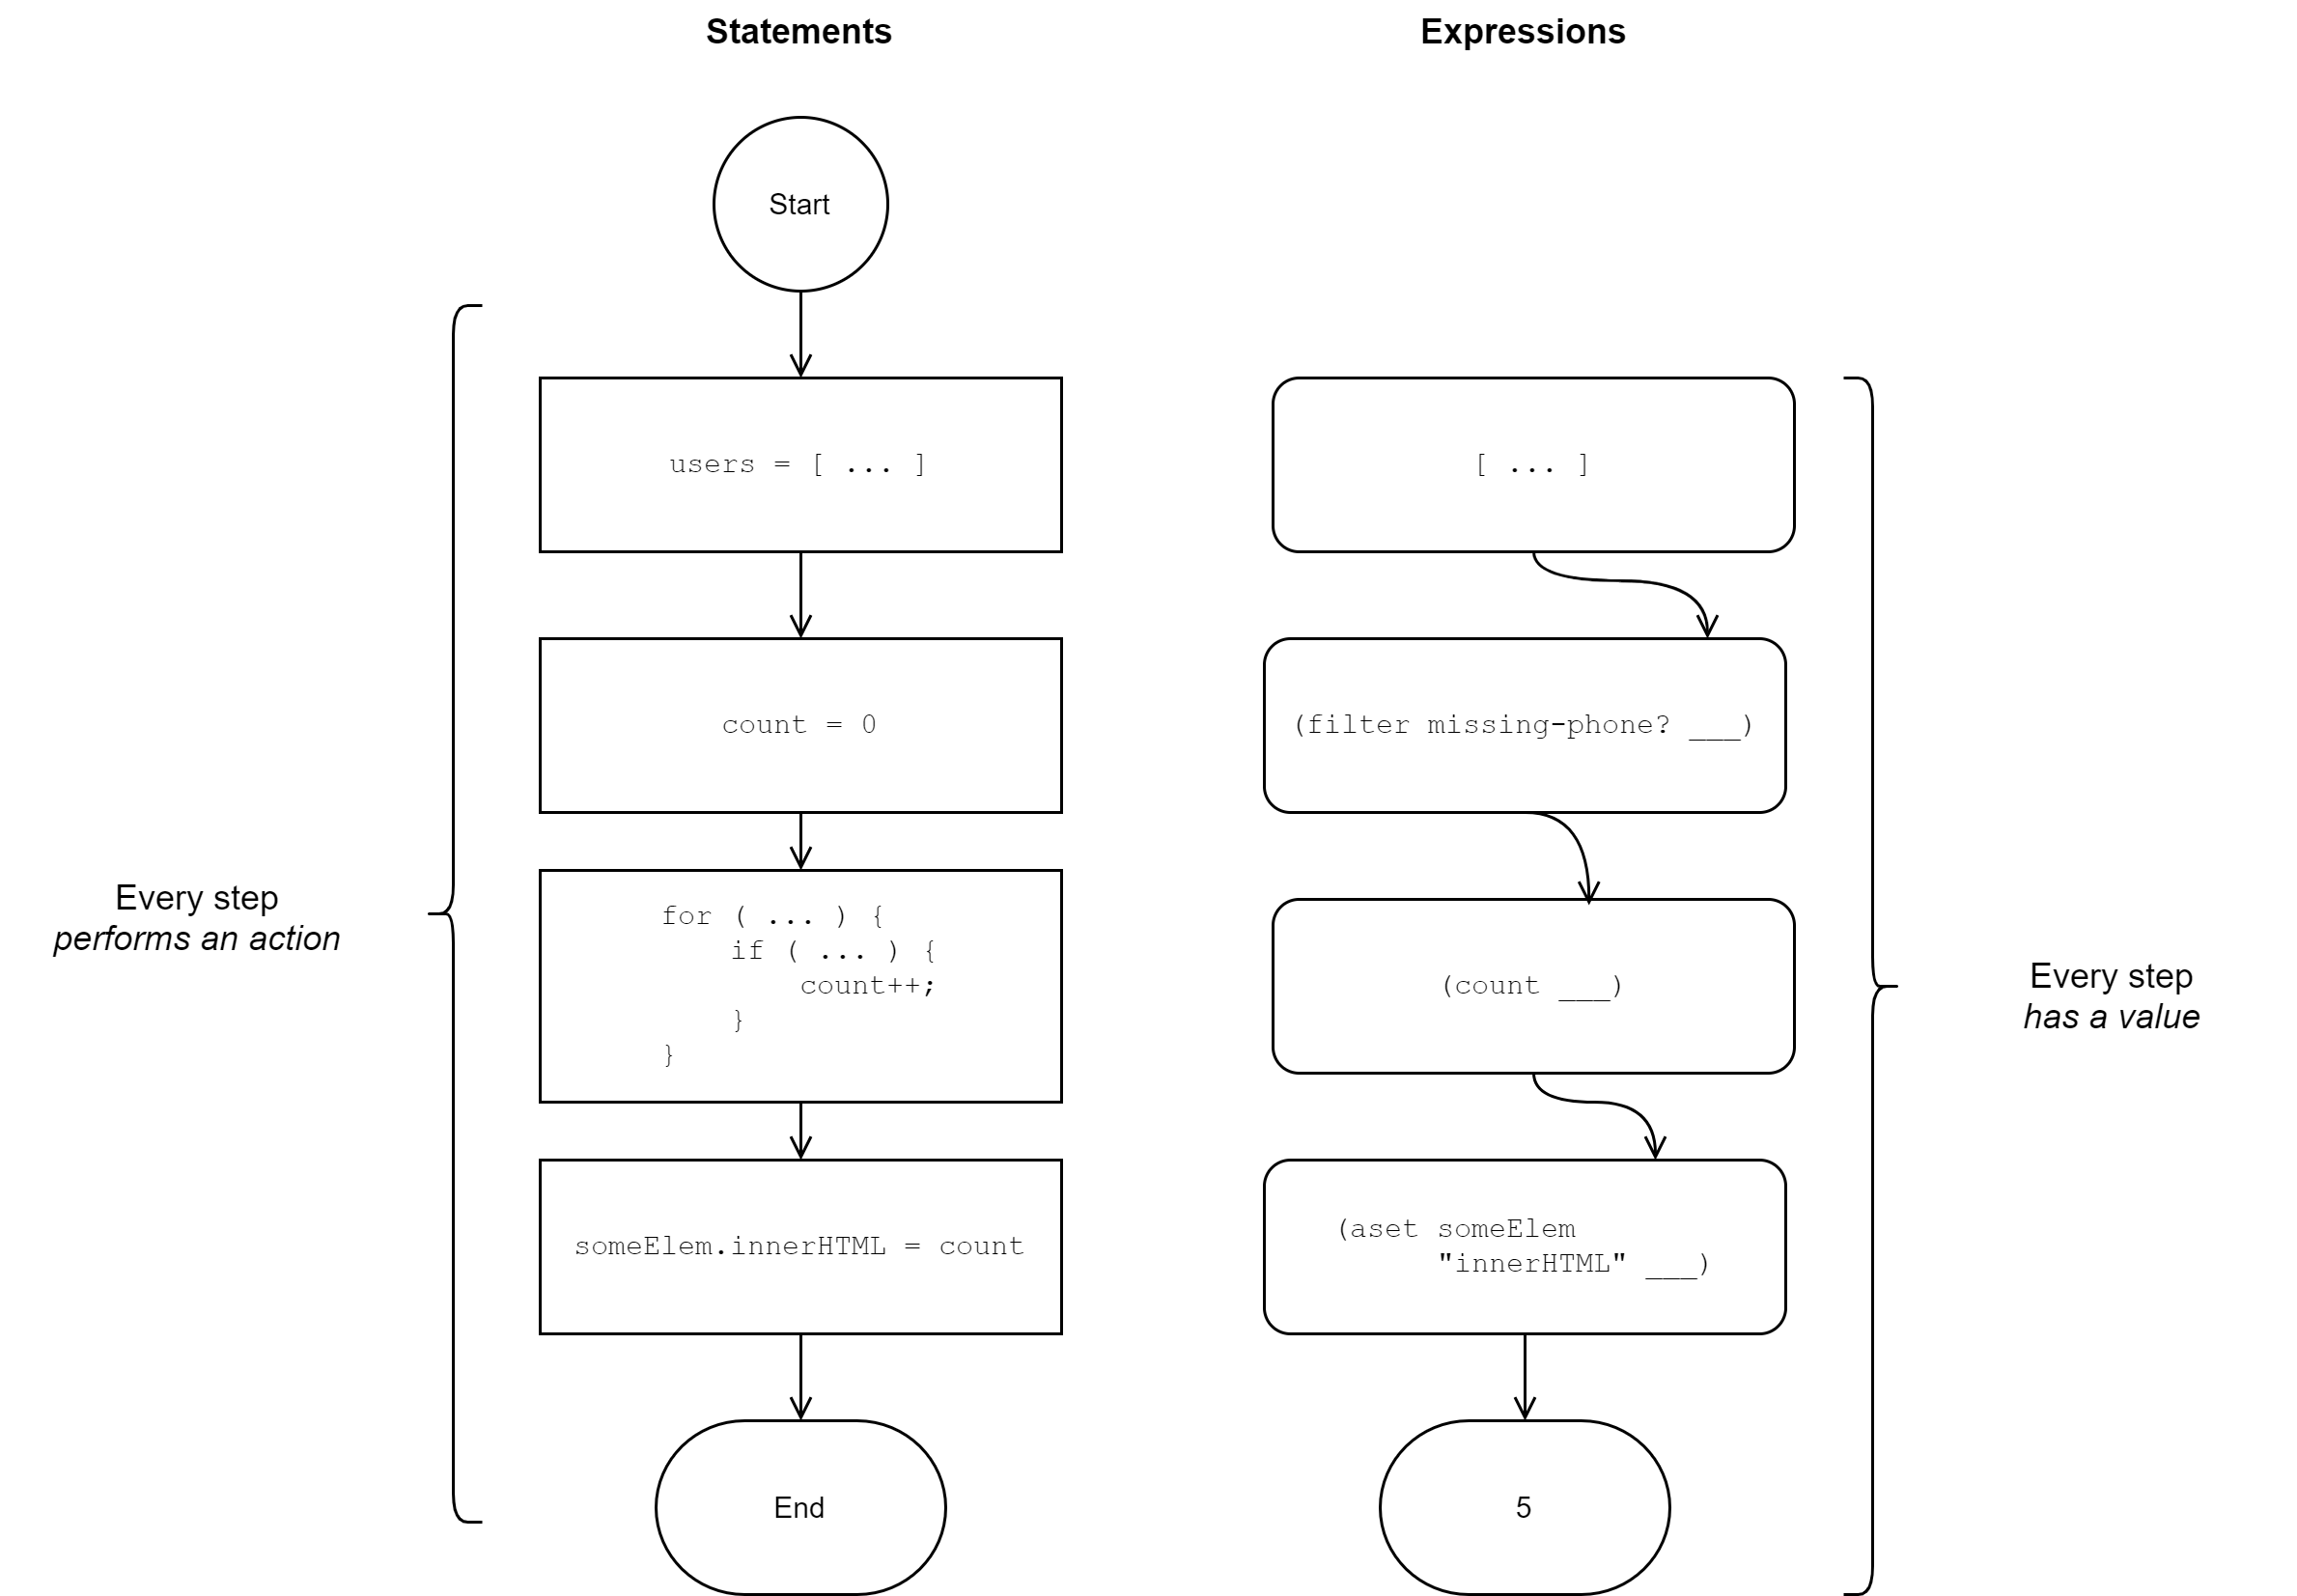
\includegraphics[width=5in]{lesson4/comparing-expressions-and-statements.png}
\end{figure}

We see that the expression-oriented code returns a value at the end.
However, since each expression is composed of other expressions, each
step in the process has some value. Now that we have a good
understanding of what expressions are and how they differ from
statements, we can dig into how ClojureScript \emph{evaluates} (derives
values) from expressions.


\subsection{Quick Review}

\begin{itemize}
\tightlist
\item
For each of the following JavaScript code snippets, identify if it is an
expression or a statement:

\begin{lstlisting}[language=Clojure]
if (age === 16) {                                           %\circled{1}%
  sweetSixteen = true;
}

console.log('Regardless');                                  %\circled{2}%

'happy birthday to you'                                     %\circled{3}%
  .split(" ")
  .map(_.capitalize)
  .join(" ");

const x = 12;                                               %\circled{4}%

count >= threshold ? 'Too High' : 'Ok';                     %\circled{5}%

function foo() {}                                           %\circled{6}%

(function () {});                                           %\circled{7}%
\end{lstlisting}

\emph{Answers:} \circled{1} - Statement; \circled{2} - Statement; \circled{3} -
Expression; \circled{4} - Statement; \circled{5} - Expression; \circled{6} -
Statement; \circled{7} - Expression
\end{itemize}

\section{Evaluating ClojureScript Code}

ClojureScript's rules for evaluating expressions are simple:

\begin{enumerate}
\def\labelenumi{\arabic{enumi}.}
\tightlist
\item
  If the expression is a primitive element or data structure, its value
  \emph{is} that element.
\item
  If the expression is a parenthesized list of expressions, the first
  expression is interpreted as a function and the rest of the
  expressions are interpreted as arguments.
\item
  Evaluate the inner expressions first and work outwards
\end{enumerate}

As an example, we will look at the expression,
\texttt{(map\ inc\ (take\ 5\ (range)))}. This s-expression is a
parenthesized list of expressions, so the first element, the symbol
\texttt{map}, is interpreted as a function with 2 arguments:
\texttt{inc} and \texttt{(take\ 5\ (range))}.

\begin{figure}[H]
\caption{Evaluating an expression: step 1}
\centering
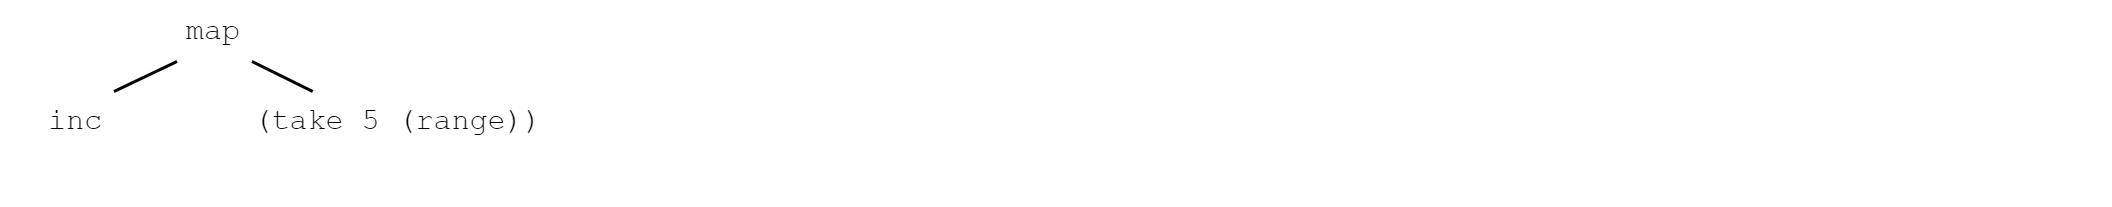
\includegraphics{lesson4/eval-step-1.png}
\end{figure}

\texttt{inc} is a function that takes an integer and returns the
next-higher number. ClojureScript can call this function\index{evaluation!of function calls} directly so
this argument does not need to be evaluated. However, the argument,
\texttt{(take\ 5\ (range))} must be evaluated so that its value can be
passed back into the \texttt{map} expression. Remembering the rules of
s-expressions, we can see the ClojureScript will interpret \texttt{take}
as a function with \texttt{5} and \texttt{(range)} as its arguments.

\begin{figure}[H]
\caption{Evaluating an expression: step 2}
\centering
\includegraphics{lesson4/eval-step-2.png}
\end{figure}

The original s-expression is almost ready to be evaluated, but first, we
must evaluate the final inner s-expression, \texttt{(range)}. This
s-expression has only a single expression inside it, \texttt{range}, so
it will be interpreted as a function with no arguments.

\begin{figure}[H]
\caption{Evaluating an expression: step 3}
\centering
\includegraphics{lesson4/eval-step-3.png}
\end{figure}

Finally, the expression will be evaluated ``inside out'', starting with
the call to the \texttt{range} function and working outwards to the
outermost s-expression.

\begin{figure}[H]
\caption{Evaluating an expression: step 4}
\centering
\includegraphics{lesson4/eval-step-4.png}
\end{figure}

The call to \texttt{range} returned an \emph{infinite} sequence of
integers, starting with \texttt{0}. We will get into how to work with
infinite sequences\index{sequences}\index{evaluation!of sequences} later, but for now, we just need to understand that
an infinite sequence is an object that can continue to produce as many
values as we need. As this expression is evaluated, the infinite
sequence is substituted in place of the original expression,
\texttt{(range)}, and the evaluation continues outwards.

\begin{figure}[H]
\caption{Evaluating an expression: step 5}
\centering
\includegraphics{lesson4/eval-step-5.png}
\end{figure}

The next expression is interpreted as a call to the \texttt{take}
function, with the arguments, \texttt{5} and an infinite sequence of
numbers. The value of this expression is the sequence,
\texttt{(0\ 1\ 2\ 3\ 4)}, the first 5 element of the infinite sequence
generated by \texttt{(range)}. The call to \texttt{take} is replaced
with this return value, and evaluation continues outwards again.

\begin{figure}[H]
\caption{Evaluating an expression: step 6}
\centering
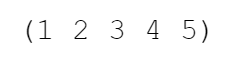
\includegraphics{lesson4/eval-step-6.png}
\end{figure}

Finally, the last step of the evaluation is performed, calling
\texttt{map} with the arguments, \texttt{inc} and
\texttt{(0\ 1\ 2\ 3\ 4)}. This increments every element in the sequence,
and returning the final value of the s-expression.

The rules of evaluating ClojureScript are simple enough that we could
work out in a few steps how an expression is evaluated. The amazing
thing about this is that no matter how large and involved the code that
we are looking at, we can use the same process to read almost any piece
of ClojureScript. Once the basic syntax is understood, most of what
remains to learn is the vocabulary and common idioms.

\section{Order of Operations}

It may come as a surprise, but ClojureScript has no concept of operator
precedence.index{operator precedence} That is, there are no rules indicating that multiplication
should be performed before addition or any such thing. Instead of having
a set of rules that implicitly determine the order in which to evaluate
an expression, we specify the order by how we nest s-expressions. For
example, the following code multiplies 5 and 2 before adding the result
to 10:

\begin{lstlisting}[language=Clojure, caption={Multiply then add}]
(+ 10 (* 5 2)) ; 20
\end{lstlisting}

On the other hand, the next bit of code adds 10 and 5 before multiplying
the result by 2:

\begin{lstlisting}[language=Clojure, caption={Add then multiply}]
(* (+ 10 5) 2) ; 30
\end{lstlisting}

The use of parentheses to determine the order of operations forces us to
be more explicit and virtually eliminates the entire class of bugs
related to operator precedence.

\subsection{You Try It}

\begin{itemize}
\tightlist
\item
  Write the expression that would call a function named
  \texttt{make-dessert} with the arguments \texttt{"ice\ cream"} and
  \texttt{"brownies"}.
\item
  Write the following mathematical expression in ClojureScript such that
  the multiplication is performed before addition and subtraction:
  \texttt{8\ +\ 3\ *\ 4\ -\ 10}.
\item
  Write same expression as the last exercise but such that the
  multiplication is performed last.
\end{itemize}

\section{Summary}

In this lesson, we learned what expressions are and how
expression-oriented programming differs from statement-oriented
programming. This led us to an examination of ClojureScript's evaluation
strategy, which simplifies expressions from the inside out. Finally, we
learned how the s-expression syntax eliminates the need for operator
precedence by making the order of every operation explicit. We can now:

\begin{itemize}
\tightlist
\item
  Understand how ClojureScript will evaluate our code
\item
  Define the difference between \emph{execution} of a set of statements
  and \emph{evaluation} of an expression
\item
  Read ClojureScript's s-expression syntax
\end{itemize}

\cleardoublepage

{\let\newpage\relax\part{Tools of the Trade}}

ClojureScript is a very productive and efficient language. While these
features stem largely from the language itself, ClojureScript owes quite
a bit of its productivity to the tools and common practices that have
developed around it (like its Lisp predecessors over the past few
decades). While there are some code samples and exercises in this
section - including a simple but complete application in
Lesson 8 -
the focus is on learning the tools that will make you an effective
ClojureScript programmer. Just as a new JavaScript developer needs a
basic understanding of Babel, Webpack, and the browser dev tools, a new
ClojureScript developer ought to have a familiarity with the tools that
we cover in this section.

Now that we have a high-level perspective on ClojureScript as a language
and its place in the JavaScript ecosystem, we will walk through the
process of bootstrapping a new ClojureScript project using the
ClojureScript compiler and its included build tooling. Next, we will
introduce Figwheel, an invaluable tool for live-reloading code and
styles, and we will learn how to write code that is conducive to live
reloading. Then, we will introduce the REPL - an extremely powerful tool
for experimenting with small snippets of code. Finally, we will use
these tools to create a weather forecasting app that showcases and live
reloading. This project is intended to convey a taste of the process of
developing ClojureScript rather than giving a deep understanding of the
code. Don't worry though: in the following section, we will begin our
exploration of the syntax and semantics of the language!

\begin{itemize}
\tightlist
\item Lesson 5: Bootstrapping a ClojureScript Project
\item Lesson 6: Receiving Rapid Feedback With Figwheel
\item Lesson 7: REPL Crash Course
\item Lesson 8: Capstone 1 - Weather Forecasting App
\end{itemize}


\chapter{Bootstrapping a ClojureScript Project}

Until this point, our discussion of ClojureScript has been largely
theoretical. We have an idea of why we would want to use ClojureScript,
but what does it look like in action? Over the course of this section,
we'll develop a small weather forecasting application from scratch. We
will pay attention to the high-level concepts while leaving the
discussion of the particulars until later. At this point, we are
interested in getting used to the look of ClojureScript code,
identifying how it makes things that are difficult in JavaScript easier,
and how the tooling helps streamline the development process. Although
the syntax of the application may still seem a bit foreign, we'll start
to get a feel for how fun and productive a ClojureScript project can be.

\begin{center}\rule{0.5\linewidth}{0.5pt}\end{center}

\textbf{In this lesson:}

\begin{itemize}
\tightlist
\item
  Walk through setting up a project from scratch
\item
  Learn how to use the ClojureScript compiler to build your code
\item
  Bootstrapping with clj-new
\end{itemize}

\begin{center}\rule{0.5\linewidth}{0.5pt}\end{center}

To start out, we will learn how to create and build a ClojureScript
project. Just as the carpenter must be familiar with all of his tools
before he can create a masterpiece, we must get acquainted to the tools
of our trade. Coming from the glut of tools\index{tooling!JavaScript} that we need for JavaScript
development, it should come as a relief that there are only a few key
tools that we need for any ClojureScript project.

\section{Meeting clj}

\index{clj}Each language has its own set of tools to learn, and ClojureScript is no
different. In this book, we will focus on two very important tools -
\texttt{clj} for general-purpose build tasks, and Figwheel\index{Figwheel} for live
reloading of code. We'll begin by looking at our new friend
\texttt{clj}, the built-in command-line tool for managing dependencies
and building code. Like JavaScript's \texttt{npm}, \texttt{clj} is a
configuration-based dependency manger as well as a simple build tool.
The reader who has some familiarity with building software projects
should feel at home rather quickly, but do not worry if this is your
first exposure to using a build process. We will walk through the
essentials in enough detail to get comfortable building ClojureScript
applications.

The Clojure language comes with a command-line tool that can be used for
compiling both Clojure and ClojureScript. While other build tools exist,
the \texttt{clj} tool is the defacto option. It is a simple tool, but it
is powerful enough to use even on a large project. We will use it for
managing dependencies, compiling, and testing our projects. Using a
single tool for all of these concerns should come as a welcome change
from the proliferation of tools in the JavaScript landscape. Before
proceeding any further, we should install Java and Clojure.\index{Clojure} Since
instructions change slightly with each release, readers are encouraged
to follow the most recent instructions at the official
Clojure Getting Started Guide\footnote{https://clojure.org/guides/getting\_started}. One interesting feature of ClojureScript is that we do
not need to install it manually - we only need to specify it as a
dependency of our project. Once Clojure is installed, we can create a
new project.

\subsection{Creating a Project Manually}

While there are tools available to create a skeleton project from a
template, we will first set up our project manually so that we can
better understand what is going on under the hood. First, we will need
to create a new directory and enter it.

\begin{verbatim}
$ mkdir my-cljs-project
$ cd my-cljs-project
\end{verbatim}

Next, we will need a \texttt{deps.edn}\index{deps.edn} file in this directory. This file
is the equivalent of a \texttt{package.json} in the JavaScript tooling
community, and it specifies the list of the dependencies that our
project requires as well as the location of our source code and script
aliases. The \texttt{.edn} extension indicates that the file uses
\emph{Extensible Data Notation}\index{EDN (extensible data notation)} - a file format containing ClojureScript
data structures. Let's create a bare-bones deps file now:

\begin{lstlisting}[language=Clojure, caption={deps.edn}]
{:deps {org.clojure/clojurescript {:mvn/version "1.10.773"}}
 :paths ["src"]}
\end{lstlisting}

The \texttt{:deps} entry contains all of the dependencies that our
project needs. In this case, we are requesting a recent (as of the time
of this writing) version of ClojureScript. Don't worry too much about
the format of the deps map, since most packages will provide you with an
entry to paste into your deps file.

The \texttt{:paths} entry instructs the ClojureScript compiler where to
look for code. If we had any tests, we would add the path to our tests
to this vector as well.

Now, let's create our first source file and compile it! Create a file
called \texttt{src/my\_cljs\_project/core.cljs}, and type in the
following contents:

\begin{lstlisting}[language=Clojure, caption={my\_cljs\_project/core.cljs}]
(ns my-cljs-project.core)                                  %\circled{1}%

(js/alert "Hello World")                                   %\circled{2}%
\end{lstlisting}

\begin{enumerate}[label=\protect\circled{\arabic*}]
\tightlist
\item Namespace declaration
\item Trigger an alert
\end{enumerate}

By default, our application will get compiled to \texttt{out/main.js},
so let's create a simple HTML page to load this application.

\begin{lstlisting}[language=HTML, caption={index.html}]
<!DOCTYPE html>
<html>
  <head>
    <meta charset="UTF-8">
  </head>
  <body>
    <script src="out/main.js" type="text/javascript"></script>
  </body>
</html>
\end{lstlisting}

Now, we will compile our ClojureScript file and load the script in a
browser. All of this can be done with one command:

\begin{verbatim}
$ clj -m cljs.main --compile my-cljs-project.core --repl
\end{verbatim}

When you run this command, you should be greeted by an empty page that
pops up a ``Hello World'' alert! Let's break this down so that we
understand what this command is doing.

\begin{itemize}
\tightlist
\item
  \texttt{clj} This invokes the Clojure command-line tool.
\item
  \texttt{-m\ clj.main} This flag specifies the function to run. When we
  included \texttt{org.clojure/clojurescript} as a dependency in the
  \texttt{deps.edn} file, it instructed \texttt{clj} to download the
  ClojureScript compiler. \texttt{clj.main} is the function that invokes
  the compiler itself. The remaining flags are interpreted by the
  ClojureScript compiler rather than \texttt{clj} itself.
\item
  \texttt{-\/-compile\ my-cljs-project.core} This specifies the
  namespace of the ``entry point'' of our application. Since we only
  have one file, we specify its namespace. Note that the namespace
  matches what we specified at the top of our \texttt{core.cljs} file.
\item
  \texttt{-\/-repl} This flag does two things: first, it launches a web
  server to serve the \texttt{index.html} file and the compiled
  JavaScript; second, it starts a REPL, an interactive interpreter that
  we will learn about in Lesson .
\end{itemize}

\begin{notice}[title={Terminal Environment}]
The terminal examples in this book are for a Unix-like\index{Unix} environment such
as OSX\index{OSX} or Linux\index{Linux}. Windows users may have to make minor adaptations the
commands.
\end{notice}

\subsection{Using Aliases}

While the \texttt{clj} tool offers us all of the options that we need to
build and run our code, it is a hassle type out
\texttt{clj\ -m\ cljs.main\ -\/-compile\ my-cljs-project.core\ -\/-repl}
every time we want to start up our application. A \texttt{deps.edn} file
lets us specify script aliases that allow us to declare a shorthand for
a number of commands or even run a Clojure file.

\begin{lstlisting}[language=Clojure, caption={deps.edn}]
;; ...
:aliases
  {:dev {:main-opts ["-m" "cljs.main"
                     "--compile" "my-cljs-project.core"
                     "--repl"]}}
\end{lstlisting}

With this alias in place, we can run our application with the following
command: \texttt{clj\ -M:dev}.

\subsection{Quick Review}

\begin{itemize}
\tightlist
\item
  What is a \texttt{deps.edn} file, and what is its equivalent in the
  JavaScript ecosystem?
\item
  Explain each of the flags that were passed to \texttt{clj} to run our
  application.
\end{itemize}

\subsection{Understanding clj}

Sticking with the Clojure philosophy of composing more advanced
functionality from small, simple pieces, \texttt{clj} is a building
block that has a well-defined purpose: managing dependencies and running
Clojure code (including the ClojureScript compiler). There are other
more fully-featured tools for project management, but with more features
come more complexity. For this book, we will be sticking with
\texttt{clj} and a tool called Figwheel\index{Figwheel}, which we will introduce in the
next lesson.

When we invoke \texttt{clj\ -m\ cljs.main\ ...}, several things happen.
First, any dependencies specified in \texttt{deps.main} will be
downloaded. This download will only happen on the initial run, and the
packages will be cached locally for subsequent runs. Second, the Java
Virtual Machine\index{Java Virtual Machine} will be started and the Clojure compiler loaded. Next,
Clojure will load the code specified by the \texttt{-m} flag. In our
case, we specify \texttt{cljs.main}, which is the entry point for the
ClojureScript compiler. This code is available to us because we added
the package for the ClojureScript compiler
(\texttt{org.clojure/clojurescript}) to \texttt{deps.edn}.

After the \texttt{-m\ cljs.main} flag, the rest of the flags are
interpreted by the ClojureScript compiler rather than \texttt{clj}
itself. We will not present a reference for the ClojureScript compiler
options here, but there is an excellent official reference\footnote{https://clojurescript.org/reference/repl-and-main}. Instead, we will
discuss the options that we need as they arise through the course of the
coming lessons.

\section{Bootstrapping a Project}

Now that we have had a whirlwind tour of \texttt{clj}, let's dive in and
create our first simple project, a weather forecasting app. We will use
a tool called clj-new\footnote{https://github.com/seancorfield/clj-new}\index{clj-new} to
create the project from a template in order to eliminate the tedium of
manually configuring everything. Just like with the ClojureScript
compiler, we can make use of clj-new without explicitly installing
anything. One additional feature of \texttt{clj} is that it allows
aliases to be defined in \texttt{\textasciitilde{}/.clojure/deps.edn}
that are always available. Go ahead and create this file with the
following contents:

\begin{lstlisting}[language=Clojure, caption={\textasciitilde{}/.clojure/deps.edn}]
{:aliases
 {:new {:extra-deps {seancorfield/clj-new
                     {:mvn/version "1.1.243"}}
        :exec-fn clj-new/create}
        :exec-args {}}}
\end{lstlisting}

This will allow us to use the command \texttt{clj\ -X:new} to invoke the
\texttt{clj-new/create} function provided by the
\texttt{seancorfield/clj-new} package. clj-new requires a template name
and a project name in order to generate the scaffolding for the project.
Since we will be using Figwheel to automatically compile code and reload
it as we make changes, we can use a clj-new \emph{template}, which is a
blueprint for the files and directory structure to create. By default
there are several built-in templates for generating Clojure applications
libraries, but we can specify other templates as well. When invoking
clj-new with a template name, it will check to see if the template is a
built-in one or one. If it cannot find a built-in template, it will try
to find the appropriate template from a central repository, download it,
and generate our project.

The Figwheel\index{Figwheel!clj-new template} project provides a template that generates a ClojureScript
project with all the plumbing required for live reloading. We will be
using the Reagent library - an idiomatic ClojureScript wrapper around
React - for building the UI, and thankfully the Figwheel template allows
us to pass an additional argument to include Reagent\index{Reagent} boilerplate code in
the generated project. We can now create the project for our app.

\begin{verbatim}
$ clj -X:new :template figwheel-main :name learn-cljs/weather :args '["+deps" "--reagent"]'
\end{verbatim}

Since this command includes some unfamiliar syntax, let's take a moment
to dissect it. As we just learned, the first part of the command,
\texttt{clj\ -X:new}, invokes the \texttt{clj-new/create} function, and
the remainder of the arguments are passed to this function. We use
Clojure keyword syntax to pass \texttt{:template}, \texttt{:name}, and
\texttt{:args} options. \texttt{:template} unsurprisingly specifies the
name of the template to use, \texttt{:name} is the name of the project
to create, and \texttt{:args} are additional arguments that the
\texttt{figwheel-main} template will interpret. Since
\texttt{figwheel-main} is not a built-in template, clj-new will fetch
the template from Clojure's central repository,
Clojars\footnote{https://clojars.org/}.\index{Clojars}


We need to understand a bit of convention in order to make sense of the
structure of the generated project. Most Clojure and ClojureScript
projects use a namespace-qualified package name to reduce the likelihood
of naming conflicts between projects that are pushed to a central
registry. The namespace is the portion before the forward slash and is
commonly the GitHub username of the developer or the reverse domain name
of the organization that owns the code, although it can be anything you
like. For this book, we will use \texttt{learn-cljs} as the namespace
for all of our projects.\footnote{You will sometimes see the namespace
  referred to as the ``groupId'' and the name as the ``artifactId''.
  This has to do with the naming conventions used by Java's Maven
  project management tool, which is what much Clojure tooling is built
  on top of.}

\begin{figure}[H]
\caption{Project namespace and name}
\centering
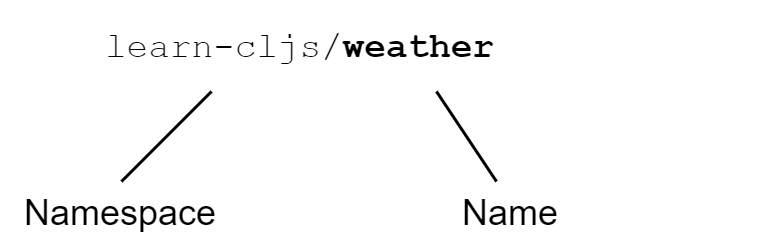
\includegraphics[width=2.54in]{lesson5/namespace-and-name.png}
\end{figure}

The final argument is a bit odd-looking:
\texttt{:args\ \textquotesingle{}{[}"+deps"\ "-\/-reagent"{]}\textquotesingle{}}.
This passes a vector of strings as arguments to the
\texttt{figwheel-main} template. The exact arguments supported vary from
template to template, but Figwheel uses these to configure optional
extensions to the base template. In our case, we are specifying that we
want to use a \texttt{deps.edn} file to manage dependencies, and we want
to include the Reagent web framework.

\section{Exploring the Project}

We now have a running (albeit skeletal) ClojureScript project. To see
the application that clj-new generated, we can navigate into the project
directory and see what files were generated.

\clearpage
\begin{verbatim}
$ cd weather
$ tree -a
.
├── .gitignore
├── README.md
├── deps.edn
├── dev.cljs.edn
├── figwheel-main.edn
├── resources
│   └── public
│       ├── css
│       │   └── style.css
│       ├── index.html
│       └── test.html
├── src
│   └── learn_cljs
│       └── weather.cljs
├── target
│   └── public
├── test
│   └── learn_cljs
│       ├── test_runner.cljs
│       └── weather_test.cljs
└── test.cljs.edn
\end{verbatim}

Let's go ahead and explore what each of these files and directories are
for. We are already familiar with the \texttt{deps.edn} file, and the
\texttt{README.md} and \texttt{.gitignore} files should be
self-explanatory, but the other EDN files could use some explanation:

\begin{itemize}
\tightlist
\item
  \texttt{dev.cljs.edn} - build file. Figwheel allows the use of
  separate build configurations that can be used to pass different
  options to the ClojureScript compiler. For example, we could use this
  file to configure development builds and use another file for
  production builds.
\item
  \texttt{figwheel-main.edn} - Figwheel configuration file. This file
  provides configuration options to Figwheel itself.
\item
  \texttt{test.cljs.edn} - build file. Like \texttt{dev.cljs.edn}, this
  file configures a specific build - in this case, the test build.
\end{itemize}

The \texttt{src} directory contains all of the ClojureScript source
files for our project. Usually, there will be a single folder under
\texttt{src} that shares the same name as our project's namespace, and
under this folder, there can be any number of \texttt{*.cljs} files and
other folders. By default, the \texttt{figwheel-main} template creates a
single \texttt{\textless{}project-name\textgreater{}.cljs} file in this
directory. If we open \texttt{weather.cljs} in a text editor or IDE\index{IDEs} that
supports ClojureScript \footnote{Most programmers' text editors have a
  Clojure language package that can be used for ClojureScript, but if
  you prefer working with IDEs, Cursive is by far the most fully
  featured Clojure(Script) IDE available.}, we will see something like
this:

\begin{figure}[H]
\caption{Editing with VS Code}
\centering
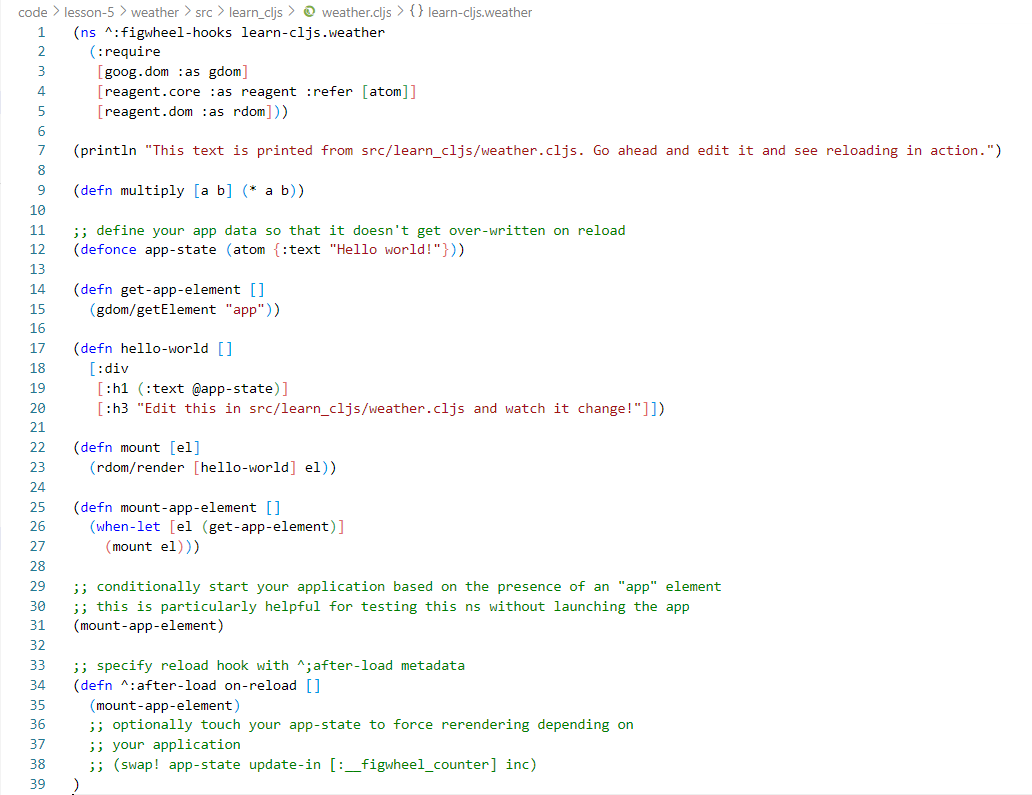
\includegraphics[width=8.73cm]{lesson5/vscode-screenshot.png}
\end{figure}

We will dig in to the rest of this file over the next couple of lessons,
as we start to build out the weather forecasting app. For now, we will
look at the namespace declaration at the top of the file, since it is
closely tied to the structure of the project. Each ClojureScript file
contains a single \emph{namespace},\index{namespace} which is simply a collection of data
and functions. The namespace is the unit of modularity in ClojureScript.
If we open up the \texttt{weather.cljs} file that was created, we can
see the namespace declared on the first line (ignoring the
\texttt{\^{}:figwheel-hooks} bit for now):
\texttt{(ns\ \^{}:figwheel-hooks\ learn-cljs.weather)}. The
ClojureScript compiler uses a simple naming convention for namespaces
based on the name of the file that houses them:

\begin{enumerate}
\def\labelenumi{\arabic{enumi}.}
\tightlist
\item
  Take the file path relative to the source directory
\item
  Replace the path separator (``/'' on Unix-like systems and ``" on
  Windows) with a dot,''."
\item
  Replace hyphens, ``-'', with underscores "\_"
\end{enumerate}

\begin{figure}[H]
\caption{Filename to namespace convention}
\centering
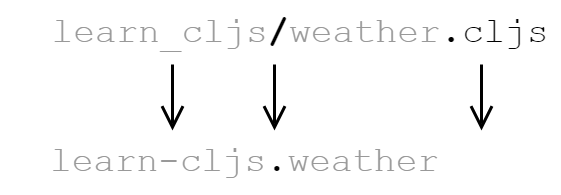
\includegraphics[width=1.87in]{lesson5/namespace-transformation.png}
\end{figure}

\begin{notice}[title={Hyphen or Underscore?}]
One detail that sometimes trips up newcomers to ClojureScript is the
fact that we name directories in the project with underscores but we
name namespaces with hyphens. This is a convention borrowed from
Clojure, which compiles namespaces into Java classes, naming the classes
according to their file path. Since hyphens are not allowed in Java
class names, they are not allowed in the file paths either.
ClojureScript follows Clojure's lead and requires that hyphens in a
namespace be converted to underscores in the filesystem path. It is a
quirk, but it is one that is easy to live with once we are aware of it.
\end{notice}

The \texttt{resources/} directory contains all of the assets that we
need to serve a website, including an \texttt{index.html}, a style sheet
(which is empty by default), and once we build our project, and a page
for hosting a test runner. The \texttt{index.html} was created with a
single div that we can load our application into, and it includes the
JavaScript file that will load our application with its dependencies.

\subsection{Quick Review}

\begin{itemize}
\tightlist
\item
  What file would you change to tweak the markup of the page that will
  load your app?
\item
  What file would you change to add project dependencies?
\item
  What file would you create to add a
  \texttt{learn-cljs.weather.sunny-day} namespace?
\end{itemize}

\section{Summary}

In this lesson, we have walked through the process of creating a new
ClojureScript project from scratch. We were introduced to clj, the
built-in Clojure (and ClojureScript) build tool. We then looked at the
\texttt{clj-new} project scaffolding tool, and we explored the project
structure that it generated for us. Next, we will learn about Figwheel,
the other core tool that will enable us to receive immediate feedback
while we are developing. After that, we will be able to jump in with
both feet and start writing code. We now know:

\begin{itemize}
\tightlist
\item
  How to set up a brand new ClojureScript project from scratch
\item
  What sort of tasks are handled by the \texttt{clj} tool
\item
  How to use \texttt{clj-new} to to bootstrap a project from a template
\item
  How a typical ClojureScript project is laid out
\end{itemize}


\chapter{Receiving Rapid Feedback With Figwheel}

In the last lesson, we only executed one command, but we already have a
basic project that will compile, and as we will see in a moment,
automatically reload. Figwheel\index{Figwheel} is the tool of choice in the
ClojureScript community for reloading code and executing ClojureScript
inside a web browser. Interactive development has been a huge priority
for ClojureScript developers, and the instant feedback afforded by a
tool like Figwheel delivers on making development a truly interactive
experience.

\begin{center}\rule{0.5\linewidth}{0.5pt}\end{center}

\textbf{In this lesson:}

\begin{itemize}
\tightlist
\item
  Learn how interactive development is a cornerstone of ClojureScript
\item
  Use Figwheel to compile and load it into the browser instantly
\item
  Learn how to write reloadable code
\end{itemize}

\begin{center}\rule{0.5\linewidth}{0.5pt}\end{center}

In order to better understand how Figwheel can streamline development,
let's fire it up and see it in action. Since we generated a project
using the clj-new with the \texttt{figwheel-main} template, it included
an alias that we can use to start Figwheel with a single command.

\begin{verbatim}
$ cd weather
$ clj -A:fig:build
[Figwheel] Validating figwheel-main.edn
[Figwheel] figwheel-main.edn is valid \(ツ)/
# ... more output ...
Opening URL http://localhost:9500
ClojureScript 1.10.773
cljs.user=>
\end{verbatim}

Figwheel will take a few seconds to start up and compile the existing
code, but once the output indicates that Figwheel is ready to connect to
our application, we can open a browser and navigate to
\texttt{http://localhost:9500} and see the running application.\index{Figwheel!connecting to browser}

\begin{figure}[H]
\caption{Reloading ClojureScript with Figwheel}
\centering
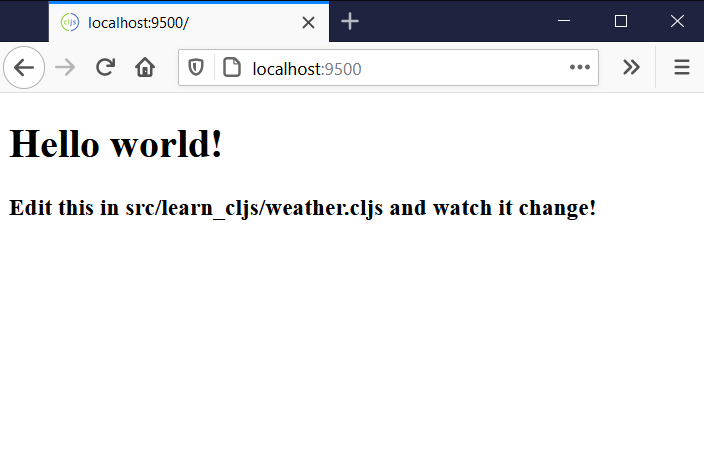
\includegraphics[width=2.347in]{lesson6/figwheel-app.png}
\end{figure}

What happens when we start Figwheel is that it begins watching our
project for any changes to the ClojureScript source files. When any of
these files are changed, Figwheel compiles them to JavaScript, sends the
JavaScript to the browser, and executes it.

\section{Testing Live Reloading}

Now that we have an application running with Figwheel reloading code on
any change, we can open a text editor and change some of the code. The
template that we used generated a single source file at
\texttt{src/learn\_cljs/weather.cljs} by default, and we will restrict
the exercises in this lesson to this single file. Before we make any
changes, let's walk through the contents of this file at a high level.

\begin{lstlisting}[language=Clojure, caption={cljs\_weather/core.cljs}]
  (ns ^:figwheel-hooks learn-cljs.weather                    %\circled{1}%
  (:require
   [goog.dom :as gdom]
   [reagent.core :as reagent :refer [atom]]
   [reagent.dom :as rdom]))

(println "This text is printed from src/learn_cljs/weather.cljs. Go ahead and edit it and see reloading in action.")

(defn multiply [a b] (* a b))

;; define your app data so that it doesn't get over-written on reload
(defonce app-state (atom {:text "Hello world!"}))          %\circled{2}%

(defn get-app-element []
  (gdom/getElement "app"))

(defn hello-world []                                       %\circled{3}%
  [:div
   [:h1 (:text @app-state)]
   [:h3 "Edit this in src/learn_cljs/weather.cljs and watch it change!"]])

(defn mount [el]
  (rdom/render [hello-world] el))

(defn mount-app-element []
  (when-let [el (get-app-element)]
    (mount el)))

;; conditionally start your application based on the presence of an "app" element
;; this is particularly helpful for testing this ns without launching the app
(mount-app-element)

;; specify reload hook with ^;after-load metadata
(defn ^:after-load on-reload []                            %\circled{4}%
  (mount-app-element)
  ;; optionally touch your app-state to force rerendering depending on
  ;; your application
  ;; (swap! app-state update-in [:__figwheel_counter] inc)
)
\end{lstlisting}

\begin{enumerate}[label=\protect\circled{\arabic*}]
\tightlist
\item Namespace declaration
\item Data structure to hold all UI state
\item Declare and render a Reagent component
\item Optional hook into Figwheel's reloading process
\end{enumerate}

Let's start by making a minor change to the \texttt{hello-world}
component. We will add a bit of extra text to it just to make sure that
our changes are picked up:

\begin{lstlisting}[language=Clojure, caption={"Hello World" component}]
(defn hello-world []
  [:div
    [:h1 "I say: " (:text @app-state)]])
\end{lstlisting}

Once we save the file, we should quickly see the browser update to
reflect the extra text that we added. Next, let's do something slightly
more interesting by changing the text inside \texttt{app-state} to
something other than ``Hello World!'':

\begin{lstlisting}[language=Clojure, caption={Changing state}]
(defonce app-state (atom {:text "Live reloading rocks!"}))
\end{lstlisting}

If we save the file again, we'll see that nothing in the browser
changes. The reason that nothing changed is that we are using
\texttt{defonce}\index{defonce@\texttt{defonce}} to create the \texttt{app-state}. Using
\texttt{defonce} ensures that whenever the \texttt{cljs-weather.core}
namespace is reloaded, \texttt{app-state} is not touched. This behavior
can give us a large productivity boost. Consider the scenario of
building a multi-page form with some complex validation rules. If we
were working on the validation for the last page in the form, we would
normally make a change to the code, reload the browser, then fill in the
form until we got to the last page, test our changes, and repeat the
cycle as many times as necessary until we had everything to our liking.
With ClojureScript and Figwheel on the other hand, we can fill in the
first few pages of the form then make small changes to the code while
observing the effects immediately. Since the app state would not get
reset when our code is re-loaded, we would never have to repeat the
tedious cycle of filling out the earlier pages.

\subsection{You Try It}

\begin{itemize}
\tightlist
\item
  Change the \texttt{hello-world} component to render a
  \texttt{\textless{}p\textgreater{}} tag instead
\item
  Create a new component called \texttt{greeter} that renders, ``Hello,
  '' and update the call to \texttt{rdom/render} to use \texttt{greeter}
  instead of \texttt{hello-world}.
\end{itemize}

\begin{notice}[title={Do I need an IDE?}]
You can edit ClojureScript in any editor or IDE that you are comfortable
with. Most modern text editors have Clojure/ClojureScript plugins that
will provide syntax highlighting and often parenthesis balancing. \index{IDEs}Some
of the more popular editors in the ClojureScript community are VS Code,
Emacs, LightTable (which is itself written largely in ClojureScript),
and vim. If you prefer an IDE, Cursive is a fully-featured
Clojure/ClojureScript IDE built on top of IntelliJ IDEA. Whether you
decide to use an IDE or simple text editor, you can find excellent
ClojureScript support.
\end{notice}

In addition to reloading ClojureScript code, Figwheel\index{Figwheel!CSS reloading} also takes care of
reloading any style sheets that we may change as well. The Figwheel
template that we used when creating this project configures Figwheel to
watch any styles in the \texttt{resources/public/css} directory for
changes. To test this out, we will open the default (empty) style sheet
and add a couple of styles:

\begin{lstlisting}[language=CSS, caption={resources/public/css/style.css}]
  body {
    background-color: #02a4ff;
    color: #ffffff;
  }
  
  h1 {
    font-family: Helvetica, Arial, sans-serif;
    font-weight: 300;
  }
\end{lstlisting}

Upon saving the style sheet, Figwheel will send the new style sheet to the
browser and apply it without a full page load. The ability to instantly
receive feedback on any ClojureScript or CSS change can lead to a very
productive workflow.


\section{Writing Reloadable Code}

Having Figwheel reload your code is a great help, but it is not magic -
we are still responsible for writing code that can be reloaded without
adversely affecting the behavior of our application. Later in this book,
we will be building several applications on React.js and a ClojureScript
wrapper called Reagent\index{Reagent}, which strongly encourage a style of coding that
is conducive to live reloading, but we should still familiarize
ourselves with what makes reloadable code so that we can still take full
advantage of live reloading whether we are using one of these frameworks
or not.

There are many considerations that go into writing reloadable code, but
they essentially boil down to three key concepts, which we will consider
as the ``Pillars of Reloadable Code'': idempotent functions,
\texttt{defonce}, and display/business logic segregation.

\begin{figure}[H]
\caption{The pillars of reloadable code}
\centering
\includegraphics[width=2.5cm]{lesson6/reloadable-pillars.png}
\end{figure}

When we write code that holds to these three pillars, we will often find
that not only do we end up with reloadable code, but our code often ends
up being much more robust and maintainable as well. With that, we'll dig
into each of these pillars and how to apply them to our code.

\subsection{Idempotent Functions}

An idempotent\index{idempotency} function is a function that will have the same effect
whether it is called once or many times. For instance, a function that
sets the \texttt{innerHTML} property of a DOM element is idempotent, but
a function that appends a child to some other element is not:

\subsubsection{Idempotent and Non-Idempotent Functions}

\begin{lstlisting}[language=Clojure]
(defn append-element [parent child]                        %\circled{1}%
  (.appendChild parent child))

(defn set-content [elem content]                           %\circled{2}%
  (set! (.-innerHTML elem) content))
\end{lstlisting}

\begin{enumerate}[label=\protect\circled{\arabic*}]
\tightlist
\item
  Non-idempotent function
\item
  Idempotent function
\end{enumerate}

The \texttt{append-element} function is definitely not idempotent
because the effect will be different when we call it 100 times than when
we call it once. The \texttt{set-content} function, on the other hand,
is idempotent - no matter how many times we call it, the result is going
to be the same. When working with live reloading, we should make sure
that any function that is called on reload is idempotent, otherwise
otherwise the side effects of that code will be run many times, leading
to undesirable results.

\subsection{You Try It}

\begin{itemize}
\tightlist
\item
  Write a version of \texttt{append-element} that is idempotent and will
  only append the child if it doesn't already exist. A possible solution
  is given below:
\end{itemize}

\begin{verbatim}
(defn append-element [parent child]
  (when-not (.contains parent child)
    (.appendChild parent child)))
\end{verbatim}

\subsection{defonce}

When we have scaffolded a Figwheel project with the \texttt{-\/-reagent}
argument, the namespace that it generates uses a construct called
\texttt{defonce} to define the application state:

\begin{lstlisting}[language=Clojure, caption={Defining once}]
(defonce app-state (atom {:text "Hello world!"}))
\end{lstlisting}
 
As we mentioned above, \texttt{defonce} is very similar to \texttt{def},
but as its name suggests, it only binds the var once, effectively
ignoring the expression on subsequent evaluations. We often define our
app state with \texttt{defonce} so that it is not overwritten by a fresh
value every time our code is reloaded. In this way, we can preserve the
state of the application along with any transient data while the
business logic of our application is reloaded.

Another useful pattern for using defonce is to protect initialization
code from running repeatedly. A \texttt{defonce} expression takes the
form: \texttt{(defonce\ name\ expr)} where \texttt{name} is a symbol
that names the var to bind and \texttt{expr} is any ClojureScript
expression. Not only does \texttt{defonce} prevent the var from being
redefined, it also prevents \texttt{expr} from being re-evaluated when
the var is bound. \index{initialization code}This means that we can wrap initialization code with a
\texttt{defonce} to guarantee that it will only be evaluated once,
regardless of how often the code is reloaded:

\begin{lstlisting}[language=Clojure, caption={Wrapping initialization code}]
(defonce is-initialized?
  (do                                                      %\circled{1}%
    (.setItem js/localStorage "init-at" (.now js/Date))
    (js/alert "Welcome!")
    true))                                                 %\circled{2}%
\end{lstlisting}

\begin{enumerate}[label=\protect\circled{\arabic*}]
\tightlist
\item
  \texttt{do} evaluates multiple expressions and takes on the value of
  the last expression
\item
  Bind \texttt{is-initialized?} to \texttt{true} once the set-up is
  complete
\end{enumerate}

In this case, we defined a var called \texttt{is-initialized?} that is
only evaluated once and is bound to the value \texttt{true} once all
initialization is complete. This is the first time that we have seen the
\texttt{do} form. \texttt{do} evaluates each expression that is passed
to it and returns the value of the final expression. It is useful when
there are side effects that we want to perform (in this case, setting a
value in \texttt{localStorage} and displaying an alert) before finally
yielding some value. Combining \texttt{do} with \texttt{defonce} is a
common pattern for ensuring that certain code will run only one time.

\subsection{Quick Review}

\begin{itemize}
\tightlist
\item
  While Figwheel is running, find the line in \texttt{core.cljs} that
  contains \texttt{(defonce\ app-state\ ...)}, change the text, and save
  the file. Does the page update? Why or why not?
\item
  Find the line in \texttt{core.cljs} that contains
  \texttt{{[}:h1\ (:text\ @app-state){]}} and change the \texttt{h1} to
  \texttt{p}. Does the page update? Why is this behavior different from
  changing the definition of \texttt{app-state}?
\end{itemize}


\subsection{Display/Business Logic Separation}

The separation of display code and business logic is good practice in
general, but it is even more important for reloadable code. Recall the
\texttt{append-element} function that we wrote several moments back when
discussing idempotent functions.

Consider that we were writing a Twitter-like application and used this
function to append a new message to some feed. There are a couple of
ways in which we could write this code, but not all of them are
conducive to live reloading. Consider the following code, which does not
separate the logic of receiving a new message from displaying it:

\begin{lstlisting}[language=Clojure, caption={Combining display and business logic}]
(defn receive-message [text timestamp]
  (let [node (.createElement js/document "div")]
    (set! (.- innerHTML node) (str "[" timestamp "]: " text))
    (.appendChild messages-feed node)))
\end{lstlisting}

In this example, we combine the logic of processing an incoming message
with the concern of displaying the message. Now let's say that we want
to simplify the UI by removing the timestamp from the display. With this
code, we would have to modify the \texttt{receive-message} function to
omit the timestamp then refresh the browser, since our new code would
not affect any messages already rendered. A better alternative would be
something like the following:

\begin{lstlisting}[language=Clojure, caption={Separating display and business logic}]
(defonce messages (atom []))                               %\circled{1}%

(defn receive-message [text timestamp]                     %\circled{2}%
  (swap! messages conj {:text text :timestamp timestamp}))

(defn render-all-messages! [messages]                      %\circled{3}%
  (set! (.- innerHTML messages-feed) "")
  (doseq [message @messages]
    (let [node (.createElement js/document "div")]
      (set! (.-innerHTML node) (str "[" timestamp "]: " text))
      (.appendChild messages-feed node))))

(render-all-messages!)                                     %\circled{4}%
\end{lstlisting}

\begin{enumerate}[label=\protect\circled{\arabic*}]
\tightlist
\item
  All messages received are stored in a \texttt{defonce}'d atom that
  will not be overwritten
\item
  The function that handles new messages is pure business logic
\item
  The function that renders messages is pure display logic
\item
  Perform a render
\end{enumerate}

In this case, we could update the \texttt{render-all-messages!}
function, and when Figwheel reloaded our code, the messages list would
remain untouched, but the display function would behave differently, and
when \texttt{render-all-messages!} is called, the display for all
messages would be updated.

\begin{notice}[title={Note}]
The implementation of the above code is inefficient, since the entire
list is re-rendered every time we call \texttt{render-all-messages!}. In
later lessons, we will use the Reagent framework to achieve similar
results much more efficiently.
\end{notice}

\subsection{Quick Review}

\begin{itemize}
\tightlist
\item
  What are the pillars of reloadable code? Why is each one of these
  important?
\item
  What is the difference between \texttt{def} and \texttt{defonce}?
\end{itemize}

\subsection{You Try It}

\begin{itemize}
\tightlist
\item
  With Figwheel running, try changing the text inside the
  \texttt{app-state} and saving the file. What happens? Would something
  different have happened if we had used \texttt{def} instead of
  \texttt{defonce}?
\item
  Introduce a syntax error in the code and see what happens in the
  browser.
\end{itemize}


\section{Summary}

In this lesson, we examined a core feature of interactive development in
ClojureScript - live reloading. We used Figwheel to reload our code
whenever it changed, and we looked at the principles behind writing code
that is reloadable. Equipped with this knowledge, we can take our
productivity to the next level and enjoy much quicker feedback than we
normally get with JavaScript. We now know:

\begin{itemize}
\tightlist
\item
  How to start Figwheel from the command line
\item
  How Figwheel reloads code when it changes
\item
  How to write code that is conducive to reloading
\end{itemize}


\chapter{REPL Crash Course}

In the previous lesson, we learned how to use Figwheel to reload code
whenever a source file changed, enabling a very quick feedback cycle. In
this lesson, we will take a first look into a tool called a REPL\index{REPL!definition of}, which
stands for \emph{Read-Eval-Print Loop} and is conceptually similar to
the JavaScript console that most browsers provide. While live reloading
is a great help when we already have a good idea of the code we need to
write, the REPL gives us an environment for writing more exploratory
code - trying out ideas and algorithms before making them part of our
project. Just like unit tests, REPL development allows us to test a
piece of code in isolation, examining its output and making sure that it
matches our expectations. However, unlike unit tests, the REPL is more
interactive and provides even quicker feedback.

\begin{center}\rule{0.5\linewidth}{0.5pt}\end{center}

\textbf{In this lesson:}

\begin{itemize}
\tightlist
\item
  Understand what a REPL is and to use it
\item
  Use Figwheel's REPL to experiment with new code
\item
  Learn how the REPL interacts with a web browser
\end{itemize}

\begin{center}\rule{0.5\linewidth}{0.5pt}\end{center}


\section{Understanding the REPL}

As we mentioned above, REPL stands for \emph{Read-Eval-Print Loop}
because it \emph{Reads} each expression that we type at the prompt,
\emph{Evaluates} that expression in the context of a web browser,
\emph{Prints} the result of that expression back at our command line.
This process is illustrated in the figure below:

\begin{figure}[H]
\caption{The Read-Eval-Print Loop}
\centering
\includegraphics{lesson7/repl-overview.png}
\end{figure}

First, the REPL waits for input from the user. Once we have input a
ClojureScript expression, it compiles the expression to JavaScript and
sends the JavaScript code to a web browser (via a WebSocket) to be
evaluated. Once the browser evaluates the JavaScript code, it sends the
result back to the REPL. Finally, the REPL prints the result and waits
for more input from the user. This loop continues until the REPL is
killed or the browser that it is connected to is closed.\index{REPL!browser connection} Remember that
the ClojureScript REPL is only in charge or the \emph{Read} and
\emph{Print} portions, and it needs a browser to perform the \emph{Eval}
step, so if you kill the browser, the REPL will not be able to evaluate
anything else until you open a browser that it can connect to again.

\clearpage

\begin{notice}[title={Note}]
\index{REPL!alternatives}There are several different REPL options with ClojureScript, but we will
be using Figwheel throughout this book. Much of the information will
apply to any REPL, but be aware that other REPLs may function slightly
differently. Notably, it is possible to run a REPL that uses either
Node.js to evaluate compiled JavaScript.
\end{notice}

Simply providing a REPL is not all that interesting. After all, Ruby and
Python have REPLs (or ``interactive interpreters''), and every modern
browser has a JavaScript REPL built into its development tools. What
makes a REPL unique for ClojureScript is that ClojureScript is a
\emph{compiled} language. That means that the REPL reads ClojureScript,
compiles it to JavaScript, evaluates the JavaScript code, and prints the
result back in the ClojureScript REPL all completely seamlessly. Other
compile-to-JavaScript languages commonly offer an online interface for
pasting in portions of code and viewing the JavaScript that the code
would compile to, but ClojureScript is in a league of its own when it
comes to giving the developer a dynamic, interactive programming
environment. Using the REPL, we can have confidence that the code does
exactly what we want it to do in the browser that we are running.


\section{Using a REPL for browser interaction}

In order to load a ClojureScript REPL, we'll use the same
\texttt{learn-cljs/weather} app that we have been using through this
unit:

\begin{verbatim}
$ cd weather
$ clj -A:fig:build
\end{verbatim}

In most cases, Figwheel will be able to open a browser tab directly, but
if it did not do so, please open a browser and visit
\texttt{http://localhost:9500} so that our REPL can connect and start
evaluating expressions.

A ClojureScript REPL instantly compiles the code that we type in to
JavaScript and evaluates it in the context of a browser. In the previous
lesson, we started Figwheel, opened a browser, and navigated to
\texttt{http://localhost:9500}. We used this setup to reload our code
every time we saved it, but Figwheel also started a REPL in the terminal
that can communicate with the web page. In order to use REPL, we can
simply start typing expressions into the terminal window where Figwheel
is running, and it will execute in the context of the page in which our
application is running. Additionally, we can interact with our
application code and even change it on the fly. A typical ClojureScript
development cycle follows these steps:


\begin{figure}[H]
\caption{REPL-Driven Development Workflow}
\centering
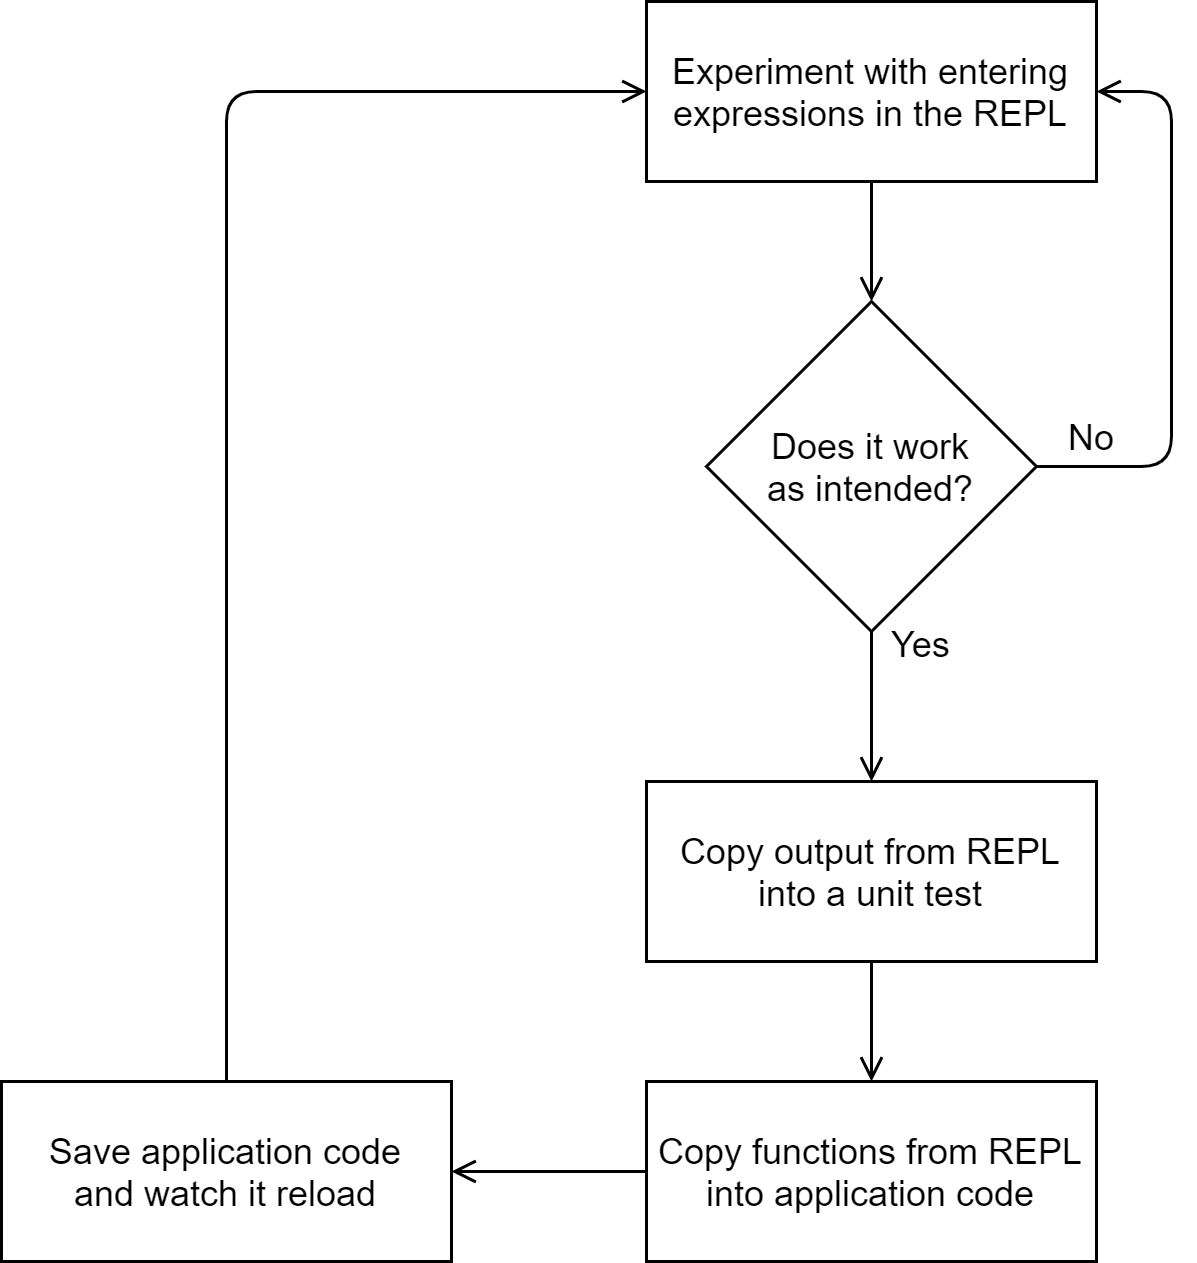
\includegraphics[width=3in]{lesson7/repl-driven-development.png}
\end{figure}

While we will not use this full workflow in this lesson, we will explore
the REPL to see how we might use it for exploratory development. Once
Figwheel is running and we have loaded our app in a browser, we should
make sure that we can see both Figwheel and the browser. Since we we
using the REPL extensively, let's take a moment to make sense of its
command-line interface:

\begin{figure}[H]
\caption{Breaking Down the REPL}
\centering
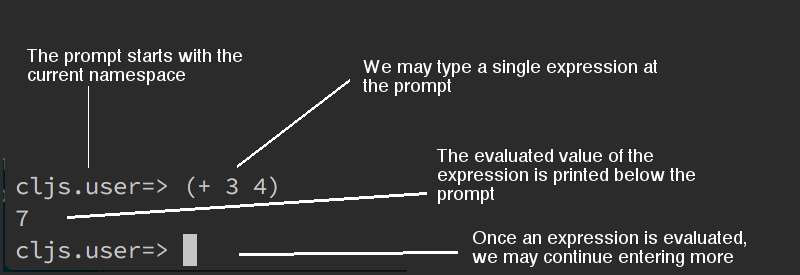
\includegraphics[width=2.66in]{lesson7/repl_breakdown.png}
\end{figure}

\index{REPL!workflow}When the REPL starts up, it will display a prompt that has the
namespace, \texttt{cljs.user}, followed by a fat arrow,
\texttt{=\textgreater{}}. As mentioned in passing earlier, the namespace
is the fundamental unit of modularity, which is used for grouping
similar functions and data together. Whenever we define functions or
data, they are added to some namespace. Unless we manually change the
namespace, anything defined at the REPL gets added to the
\texttt{cljs.user} namespace so that we do not accidentally overwrite
the code powering the running application. After this prompt, we can
start inputting expressions one at a time. An expression can span
multiple lines, but as soon as we conclude the expression, the REPL will
evaluate it and display the result on the next line. There are some
expressions that are only run for side effects and have no meaningful
value, such as \texttt{(println\ "Side\ effects!")}. In this case, the
REPL will print the string, ``Side effects!'', and return \texttt{nil},
indicating that the expression itself has no value.

\begin{notice}[title={Strings in the REPL}]
Note that the REPL displays special characters as they were entered
complete with backslash, but if we print the string with
\texttt{println}, the special characters are printed in the intended
manner for display:

\begin{verbatim}
cljs.user=> "New\nLine"
"New\nLine"

cljs.user=> (println "New\nLine")
New
Line
nil
\end{verbatim}
\end{notice}

In order to change to a different namespace, we can use the
\texttt{in-ns} function. This function takes as an argument a
\emph{symbol} with the name of the namespace to enter and changes the
REPL's environment to that namespace. For example, to change into the
main namespace of our application, we can simply enter
\texttt{(in-ns\ \textquotesingle{}learn-cljs.weather)}. \footnote{Recall from Lesson 3 that a symbol must be quoted if we do not want ClojureScript to interpret it as a name for some var.} To draw an
analogy to a filesystem, a namespace is like a directory, defining a var
with \texttt{def} or \texttt{defn} is like creating a new file, and
\texttt{in-ns} is like using \texttt{cd} to change into a new directory.
Once in the new namespace, we have access to all the vars defined in it,
and any new vars that we define will be defined in that namespace.


\subsection{You Try It}

\begin{itemize}
\tightlist
\item
  Start a Figwheel REPL from the command line
\item
  Enter some basic expressions - remember that things like numbers and
  strings are expressions.
\item
  Enter the \texttt{learn-cljs.weather} namespace, then return to the
  \texttt{cljs.user} namespace.
\end{itemize}

\subsection{Running Code in a Browser}

Notice that when we start Figwheel, it opens a web browser before it can
load a REPL. Why did we need a browser to use a REPL? Figwheel itself
does not execute the ClojureScript code. Instead, it orchestrates the
process of compiling the code to JavaScript, sending it to the web
browser for execution using the browser's JavaScript engine, then
displaying the results back in the terminal window.

\begin{figure}[H]
\caption{Figwheel client/server communication}
\centering
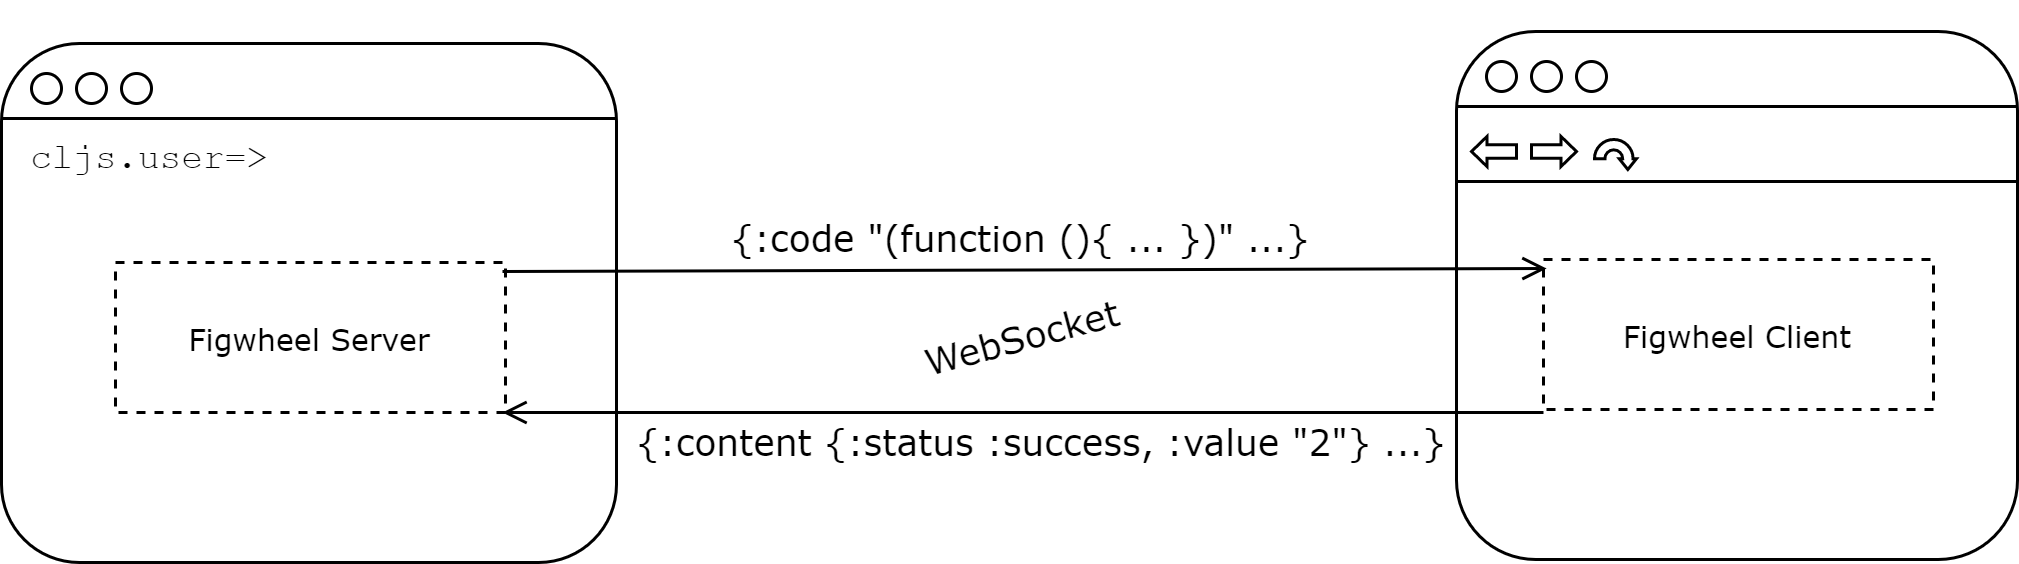
\includegraphics{lesson7/figwheel-overview.png}
\end{figure}

When we enter an expression in the REPL, Figwheel invokes the
ClojureScript compiler to generate a piece of JavaScript code. It then
sends this JavaScript code over a WebSocket\index{WebSocket} to the web browser, which
the browser evaluates and passes back over the WebSocket to the Figwheel
server. If there are any exceptions raised while running the compiled
JavaScript, the error output is sent back to Figwheel for us to look at.

This may seem like unnecessary indirection, but it is actually very
useful for a couple of reasons. First, we can have confidence that our
code will actually do the right thing in the context of a web browser,
and second, we can manipulate the browser directly from the Figwheel
REPL. We will now try a few more examples, this time with some DOM
manipulation.

\begin{lstlisting}[language=Clojure, caption={Browser interaction from the REPL}]
(in-ns 'learn-cljs.weather)                                %\circled{1}%
;; nil

(def input (.createElement js/document "input"))           %\circled{2}%
;; #'learn-cljs.weather/input                              %\circled{3}%

(.appendChild (.-body js/document) input)
;; #object[HTMLInputElement [object HTMLInputElement]]

(set! (.-placeholder input) "Enter something")             %\circled{4}%
;; "Enter something"

(defn handle-input [e]                                     %\circled{5}%
  (swap! app-state assoc :text (-> e .-target .-value)))
;; #'learn-cljs.weather/handle-input

(set! (.-onkeyup input) handle-input)
;; #object[learn_cljs$weather$handle_input ...]
\end{lstlisting}

\begin{enumerate}[label=\protect\circled{\arabic*}]
\tightlist
\item
  Enter our app's main namespace
\item
  Create an \texttt{input} element and add it to the DOM
\item
  \texttt{def} evaluates to the var that was defined
\item
  Change the \texttt{placeholder} property of the element
\item
  Create an event handler and attach it to the \texttt{input}. Note that
  this expression spans multiple lines.
\end{enumerate}

After evaluating all of these expressions in the REPL, we will have a
heading and an input in our app, and whenever we type something in it,
the \texttt{h1} will be updated with whatever we type. This is powerful
because now we have some code that we know works, and we could simply
copy statements from our REPL session and paste them into our
application. However, we could even do some refactoring in the REPL
before pasting the code into our application. Whenever we redefine
something in the REPL, it will affect the running application, so there
is no need to refresh the page before we start redefining code. However,
if we have added any event listeners or have otherwise modified the DOM,
we may want to refresh the page to return to a ``clean slate''. In our
case, we will only be refactoring the \texttt{handle-input} function, so
we can continue without reloading the page.

\subsection{Quick Review}

\begin{itemize}
\tightlist
\item
  In your words, explain what happens after you input
  \texttt{(+\ 40\ 2)} in the REPL and hit enter.
\item
  Look up \texttt{https://clojuredocs.org/} and try running some of the
  examples in the REPL. Most of ClojureScript's library is identical to
  Clojure's, so most of the examples will work the same in either
  language.
\end{itemize}

\begin{notice}[title={Important}]
Anything that we have defined in the REPL will only last until we close
or refresh the web browser, so if we want to discard everything that we
have defined in the REPL, we can simply refresh the browser. Conversely,
when in the middle of an involved REPL session, we should take care to
not refresh the browser, lest we lose the state that we have built up.
\end{notice}

We will probably want to get the value of some input that triggered an
event in multiple places, so we can extract that into its own function.
We can also make the intent of the event handler clearer if we extract
the updating of the app state into its own function as well.

\begin{lstlisting}[language=Clojure, caption={Refactored code}]
(defn event-value [e] (-> e .-target .-value))
;; #'learn-cljs.weather/event-value

(defn update-text [value]
  (swap! app-state assoc :text value))
;; #'learn-cljs.weather/update-text

(defn handle-input [e]
  (update-text (event-value e)))
;; #'learn-cljs.weather/handle-input
\end{lstlisting}

From this short REPL section, we now have some clean, refactored code
that we could use in our application. Almost all code needs to be
refactored, but the REPL-driven style of development enables us to
refactor very early in the development process so that by the time we
write a unit test or paste the code from the REPL into an application,
it is already clean and concise. The earlier we are able to clean up our
code, the less technical debt we accumulate, and ultimately, the more
productive our development becomes.

\section{Summary}

In this lesson, we explored how to use the REPL to interact with a web
page. We used it both to try out new code and to interact with code in
our application's main namespace. As with any skill, practice is key to
developing the competence that eventually leads to mastery, and
ClojureScript's REPL is one of the best ways to practice new skills.
Moving forward, we will introduce almost every topic with a REPL
session. We can now:

\begin{itemize}
\tightlist
\item
  Start a Figwheel REPL from the command line
\item
  Understand how code entered in the REPL gets evaluated
\item
  Write and refactor code in the REPL before committing it to our
  project
\end{itemize}

\chapter{Capstone 1 - Weather Forecasting App}

Over the past couple of lessons, we have been getting familiar with the
most common tools for the ClojureScript developer. While we have written
a smattering of code, the focus has been on the project itself. This
lesson will change course slightly and focus on writing a minimal app.
This lesson will be a bit more difficult, and we will gloss over most of
the detail of the code. The intent here is to present a picture of what
a typical ClojureScript development workflow looks like without getting
into the nitty-gritty details of the code. After learning the basic
syntax and idioms of the language, we should be able to come back to
this lesson with a much deeper understanding of what is going on.

\begin{center}\rule{0.5\linewidth}{0.5pt}\end{center}

\textbf{In this lesson:}

\begin{itemize}
\tightlist
\item
  Apply our knowledge of ClojureScript tools to create a new project
\item
  Develop a ClojureScript application with a REPL-driven workflow
\item
  Get a taste of the Reagent framework
\end{itemize}

\begin{center}\rule{0.5\linewidth}{0.5pt}\end{center}

In this lesson, we'll take the skills that we have learned over the past
few lessons and put them to use developing a simple weather forecasting
app that will accept user input, get data from a third-party API, and
make use of React and the \emph{Reagent}\index{Reagent} ClojureScript library for
efficient rendering. This app will be simple enough to understand with
only a minimal knowledge of ClojureScript yet will be representative
enough to give us a clear picture of ClojureScript development. With
that, let's roll up our sleeves and start writing code!

\begin{figure}[H]
\caption{A ClojureScript single-page app in action}
\centering
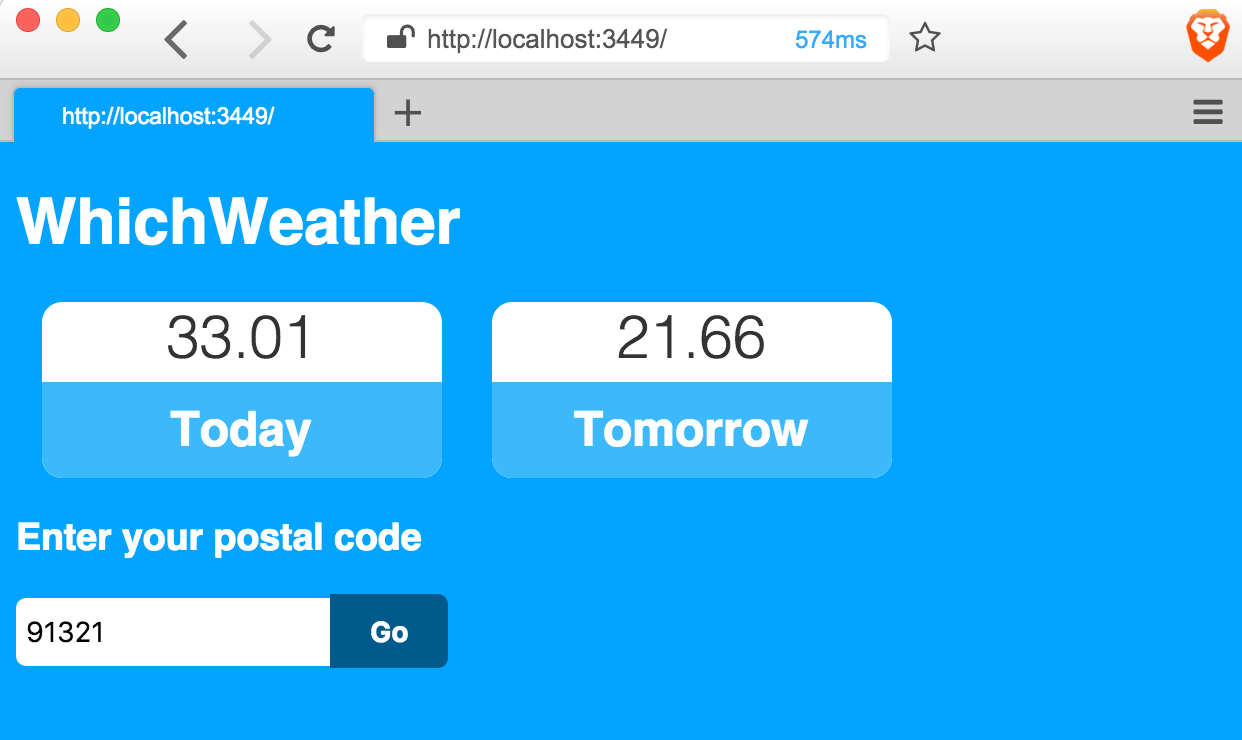
\includegraphics[width=4.14in]{lesson8/complete_app.png}
\end{figure}

\section{Creating an App With Reagent}

We have seen how a typical ClojureScript application is laid out, and we
have used clj-new to bootstrap a ClojureScript project. We have also
explored the live reloading functionality and REPL that Figwheel
provides to quickly iterate on small pieces of code. We will complete
this high-level introduction to ClojureScript development by walking
through a simple ClojureScript app. We will return to the application
that we generated. We will see how quickly we can compose a
ClojureScript application. The complete code for this lesson is
available at the book's GitHub repository\footnote{https://github.com/kendru/learn-cljs}, so feel free to simply pull the code and follow
along. The goal here is not to learn the ins and outs of ClojureScript
as a language but rather to get a feel for what production ClojureScript
looks like.

\subsection{Creating Reagent Components}

Let's begin by simplifying the core namespace so that it only contains a
single Reagent component and renders it.

\begin{lstlisting}[language=Clojure, caption={learn\_cljs/weather.cljs}]
(ns ^:figwheel-hooks learn-cljs.weather                    %\circled{1}%
  (:require
   [goog.dom :as gdom]
   [reagent.dom :as rdom]
   [reagent.core :as r]))

(defn hello-world []                                       %\circled{2}%
  [:div
   [:h1 {:class "app-title"} "Hello, World"]])

(defn mount-app-element []                                 %\circled{3}%
  (rdom/render [hello-world] (gdom/getElement "app")))
(mount-app-element)

(defn ^:after-load on-reload []                            %\circled{4}%
  (mount-app-element))
\end{lstlisting}

\begin{enumerate}[label=\protect\circled{\arabic*}]
\tightlist
\item
  Declare the namespace and load the Reagent framework
\item
  Declare a simple Reagent component
\item
  Render the Reagent component to the DOM
\item
  Instruct Figwheel to re-mount the app whenever reloading code
\end{enumerate}

Most ClojureScript user interfaces prioritize declarative components.
That is, components describe how they should render rather than
manipulating the DOM directly. The \texttt{hello-world} component in our
application looks something like Clojurized HTML. In fact, the syntax of
Reagent components is designed to emulate HTML using ClojureScript data
structures. Like with other aspects of ClojureScript, Reagent encourages
small components that can be combined from small structures into larger,
more useful pieces.

This \texttt{hello-world} component is simply a function that returns a
ClojureScript data structure. Imagining a JavaScript equivalent of this
function is straightforward:

\begin{lstlisting}[language=JavaScript, caption={A similar component in JavaScript}]
const helloWorld = () => {
    return ["h1", {"class": "title"}, "Hello, World"];
};
\end{lstlisting}

Before moving on, we should remove the \texttt{"test"} directory from
the \texttt{:watch-dirs} entry in our build configuration:

\begin{lstlisting}[language=Clojure, caption={dev.cljs.edn}]
^{:watch-dirs ["src"] ;; Previously contained "test" as well
  :css-dirs ["resources/public/css"]
  :auto-testing true
   }
{:main learn-cljs.weather}
\end{lstlisting}

We must remove the test directory because the scaffolded test contains a
test case for a \texttt{multiply} function that we removed from the
\texttt{learn-cljs.weather} namespace. If we did not remove this watch,
Figwheel would not reload our code.

\subsection{Quick Review}

\begin{itemize}
\tightlist
\item
  The \texttt{hello-world} component now has a class of
  \texttt{app-title}. Add an id attribute to the component as well and
  use your browser's development tools to verify that the change worked.
\end{itemize}


\subsection{Managing State in an Atom}

Reagent runs this function and turns it into a structure that parallels
the structure of the DOM. Any time that the function returns a different
value, Reagent re-renders the component. However, in the case of this
component, everything is static. For a component to be dynamic, it must
render some data that could change. In Reagent, we keep all of the data
that we use to render the app inside an atom\index{data types!atom}, which is simply a
container for data that might change. We have already seen an atom in
use in the boilerplate code that we scaffolded in Lesson 5:

\begin{verbatim}
(defonce app-state (r/atom {:text "Hello world!"}))
\end{verbatim}

Any Clojure data structure can be wrapped in an atom simply by wrapping
it with \texttt{(atom\ ...)}. Reagent components that make use of an
atom will automatically re-render whenever the data inside the atom
changes. This automatic re-rendering process is what enables us to write
declarative components without worrying about tedious DOM manipulation.

For the weather forecasting app, we will keep the entire app state
inside an atom wrapping a ClojureScript map: \texttt{(atom\ \{\})}. This
will enable us to manage all of the data that we will need in a single
location. This approach, when contrasted with the various approaches for
managing data in some of the most popular JavaScript frameworks, is
quite simple. The state for our weather forecast app will be quite
simple, consisting of a title, a postal code that will be entered by the
user, and several temperatures that we will retrieve from a remote API.
We can create a skeleton of this app state in the
\texttt{cljs-weather.core} namespace.

\begin{lstlisting}[language=Clojure, caption={Initial application state}]
(defonce app-state (r/atom {:title "WhichWeather"
                            :postal-code ""
                            :temperatures {:today {:label "Today"
                                                   :value nil}
                                           :tomorrow {:label "Tomorrow"
                                                      :value nil}}}))
\end{lstlisting}


With the basic data structure in place we can identify and define the
components that will make up our interface:

\begin{figure}[H]
\caption{The components of our app}
\centering
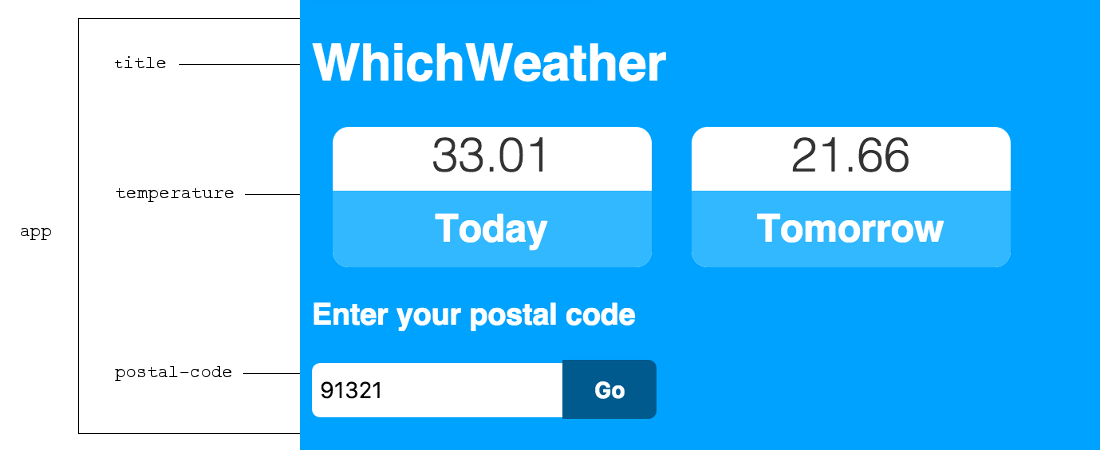
\includegraphics[width=3.667in]{lesson8/components_annotated.png}
\end{figure}

\begin{lstlisting}[language=Clojure, caption={Reagent components}]
(defn title []
  [:h1 (:title @app-state)])

(defn temperature [temp]                                   %\circled{1}%
  [:div {:class "temperature"}
   [:div {:class "value"}
    (:value temp)]
   [:h2 (:label temp)]])

(defn postal-code []
  [:div {:class "postal-code"}
   [:h3 "Enter your postal code"]
   [:input {:type "text"
            :placeholder "Postal Code"
            :value (:postal-code @app-state)}]
   [:button "Go"]])

(defn app []
  [:div {:class "app"}
   [title]                                                 %\circled{2}%
   [:div {:class "temperatures"}
    (for [temp (vals (:temperatures @app-state))]          %\circled{3}%
      [temperature temp])]
   [postal-code]])

(defn mount-app-element []                                 %\circled{4}%
  (rdom/render [app] (gdom/getElement "app")))
\end{lstlisting}

\begin{enumerate}[label=\protect\circled{\arabic*}]
\tightlist
\item
  A Reagent component that expects \texttt{temp} to be passed in
\item
  Nesting a component inside another component
\item
  Render a \texttt{temperature} component from each of the
  \texttt{:temperatures} in the app state
\item
  Instruct Reagent to render \texttt{app} instead of the
  \texttt{hello-world} component
\end{enumerate}


\section{Responding to User Input}

Now that we have an app running and rendering data, the next step is to
let the user interact with the page. We will allow the user to input
their postal code so that we can fetch weather data for their location.
As we would in JavaScript, we attach an event handler to the input
element. This handler will update the app state on every keystroke. The
\texttt{postal-code} component already gets it value from the app state.
The only step that we need to take is to attach the handler, and the
input will stay synchronized.

\begin{lstlisting}[language=Clojure, caption={Handling input with Reagent}]
[:input {:type "text"
         :placeholder "Postal Code"
         :value (:postal-code @app-state)
         :on-change #(swap! app-state assoc :postal-code (-> %\%% .-target .-value))}]
\end{lstlisting}

Note that this flow is different from the ``2-way'' data binding\index{data binding!2-way} of
JavaScript frameworks like Vue\index{Vue} or Angular 1. For example, to achieve a
similar effect in AngularJS, we would create a controller that manages
some piece of state called \texttt{postalCode} and bind this state to an
input. Internally, the framework ensures that whenever the state is
updated, the input element is updated with the new value, and whenever
the input value is changed by the user, the state is updated. Since the
framework ensures that changes propagate in the direction of UI to model
as well as model to UI, it is termed 2-way binding.

\begin{lstlisting}[language=HTML, caption={Handling input with AngularJS}]
<div ng-app="whichWeather" ng-controller="inputCtrl">      %\circled{1}%
  <input ng-model="postalCode">                            %\circled{2}%
</div>

<script>
var app = angular.module('whichWeather', []);              %\circled{3}%
app.controller('inputCtrl', function($scope) {
    $scope.postalCode = '';                                %\circled{4}%
});
</script>
\end{lstlisting}

\begin{enumerate}[label=\protect\circled{\arabic*}]
\tightlist
\item
  Provide indicators in our markup so that the framework knows which
  state to manage in the child elements.
\item
  Create an input element and declare the state that it is bound to
\item
  Create an app and controller to handle data and process interactions
\item
  Initialize the state that will be bound to the input
\end{enumerate}

While 2-way binding is convenient for very simple applications, it tends
to have performance issues, and it can be more difficult for large
applications with a lot of state, particularly derived data. The
approach that we will be taking in most of the applications in this book
is a little different and in fact, simpler. Instead of automatically
syncing the application state and the UI in a bidirectional fashion,
Reagent (and the underlying React framework) only updates the UI when
the underlying state changes. Thus, we describe our components in terms
of our data model, update that model when we receive input, and let the
framework ensure that the UI reflects the new state.

\begin{figure}[H]
\caption{Data binding strategies}
\centering
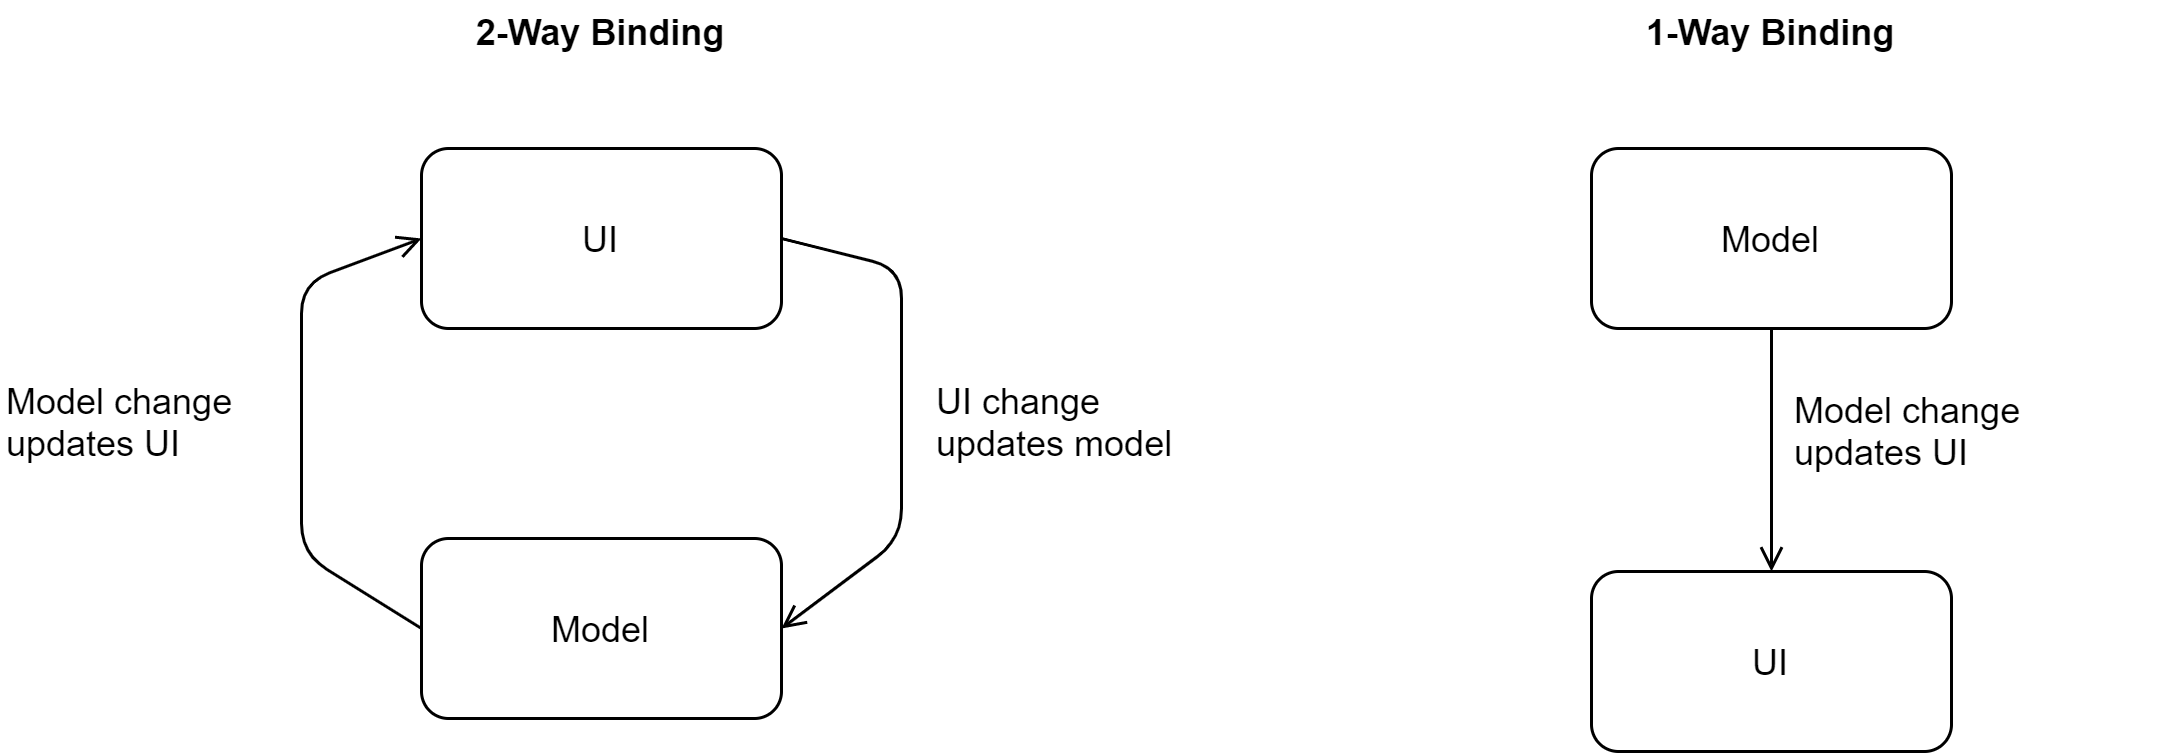
\includegraphics[width=10cm]{lesson8/data-binding-strategies.png}
\end{figure}


\index{data binding!1-way}With the one-way data binding, the model is considered the single source
of truth, and all changes to the model are explicit. While this may seem
like an inconvenience when compared to the more automatic 2-way binding,
it is much easier to reason about and debug, and it enables much simpler
logic in larger applications.


\subsection{Quick Review}

\begin{itemize}
\tightlist
\item
  Let's assume that the postal code should always be a number. Change
  the component to use an HTML5 \texttt{number} input type.
\item
  Two way data binding actively updates a model whenever some input
  changes and also updates the view when the model changes. Explain how
  this process is different.
\end{itemize}

In order to verify that the input is actually updating the app state, we
can use the REPL to inspect the current value of the app-state. Although
the name of the app state variable is \texttt{app-state}, the UI
components refer to it as \texttt{@app-state}. We will explore this
operator in great detail later, but for our purposes now, we need to
know that it will extract the current value of an atom. We can use this
operator from the REPL just as we would from a UI component to view the
current app state.

\begin{verbatim}
@learn-cljs.weather/app-state
;; {:title "WhichWeather", :postal-code "81235", :temperatures
;;  {:today {:label "Today", :value nil}, :tomorrow {:label "Tomorrow", :value nil}}}
\end{verbatim}

\section{Calling an External API}

The final piece of our weather forecast app is getting data from a
remote API. While it is entirely possible to make an Ajax\index{AJAX} request using
only the Google Closure libraries that are built in to ClojureScript,
using an external library will greatly simplify the process. We simply
need to add the \texttt{cljs-ajax} library to the \texttt{:deps} section
of \texttt{deps.edn} and restart Figwheel. At that point, we can require
the library in our namespace and start making requests.


\begin{lstlisting}[language=Clojure, caption={deps.edn}]
{:deps {org.clojure/clojure {:mvn/version "1.10.0"}
        org.clojure/clojurescript {:mvn/version "1.10.773"}
        reagent {:mvn/version "0.10.0" }
        cljs-ajax {:mvn/version "0.8.1"} ;; Added
        }
  ;; ...
}
\end{lstlisting}

For the purpose of this application, we will use \index{OpenWeatherMap}OpenWeatherMap's
forecast data API. Use of the API is free, but
an account is required to obtain an API key\footnote{https://home.openweathermap.org/users/sign\_up}.

With just 2 additional functions, we can enable communication with a
remote API and hook the results into our user interface. While there is
some unfamiliar ground in the code ahead, we can quickly understand the
basics. First, we'll consider how to process the results from the
OpenWeatherMap API:

\begin{lstlisting}[language=Clojure, caption={Handling the response}]
(defn handle-response [resp]
  (let [today (get-in resp ["list" 0 "main" "temp"])       %\circled{1}%
        tomorrow (get-in resp ["list" 8 "main" "temp"])]
    (swap! app-state                                       %\circled{2}%
        update-in [:temperatures :today :value] (constantly today))
    (swap! app-state
        update-in [:temperatures :tomorrow :value] (constantly tomorrow))))
\end{lstlisting}

\begin{enumerate}[label=\protect\circled{\arabic*}]
\tightlist
\item
  Extract data from the response
\item
  Update the app state with the retrieved data
\end{enumerate}

There are 2 pieces of data that we care about the data that the API
provides - the current temperature and the forecasted temperature for 1
day in the future. \texttt{handle-response} takes care of extracting
these pieces of data nested deep in the response and updates the values
for today's and tomorrow's temperatures in the app state. Next, we'll
look at the code necessary to make the remote API request.

\begin{lstlisting}[language=Clojure, caption={Performing a request}]
(defn get-forecast! []
  (let [postal-code (:postal-code @app-state)]             %\circled{1}%
    (ajax/GET "http://api.openweathermap.org/data/2.5/forecast"
         {:params {"q" postal-code
                   "appid" "API_KEY"
                   "units" "imperial"}
          :handler handle-response})))                     %\circled{2}%
\end{lstlisting}

\begin{enumerate}[label=\protect\circled{\arabic*}]
\tightlist
\item
  Get the postal code from the \texttt{app-state} and supply it as an
  API request parameter
\item
  Handle the response with the \texttt{handle-response} function above
\end{enumerate}

In the \texttt{get-forecast!} function, we extract the
\texttt{postal-code} from our app state in order to request a localized
forecast from the OpenWeatherMap API. Notice that we specify the
\texttt{handle-response} function as the response handler, so when the
API returns data, we will process it and update the app state
accordingly. Finally, we want to create a UI component that the user can
use to fetch data. In our case, we'll use a simple button that will
initiate the API request when clicked:

\begin{verbatim}
[:button {:on-click get-forecast!} "Go"]
\end{verbatim}

We simply attach the \texttt{get-forecast!} function as an event handler
on a button, and our work is done. The entire code from this lesson is
printed below for reference. In order to correctly communicate with the
API, please replace \texttt{"API\_KEY"} in the listing below with the
actual key from your OpenWeatherMap account.

\begin{lstlisting}[language=Clojure, caption={Complete weather forecasting app}]
(ns %\textasciicircum%:figwheel-hooks learn-cljs.weather
  (:require
   [goog.dom :as gdom]
   [reagent.dom :as rdom]
   [reagent.core :as r]
   [ajax.core :as ajax]))

(defonce app-state (r/atom {:title "WhichWeather"          %\circled{1}%
                            :postal-code ""
                            :temperatures {:today {:label "Today"
                                                   :value nil}
                                           :tomorrow {:label "Tomorrow"
                                                      :value nil}}}))

(def api-key "API_KEY")

(defn handle-response [resp]                               %\circled{2}%
  (let [today (get-in resp ["list" 0 "main" "temp"])
        tomorrow (get-in resp ["list" 8 "main" "temp"])]
    (swap! app-state
           update-in [:temperatures :today :value] (constantly today))
    (swap! app-state
           update-in [:temperatures :tomorrow :value] (constantly tomorrow))))

(defn get-forecast! []                                     %\circled{3}%
  (let [postal-code (:postal-code @app-state)]
    (ajax/GET "http://api.openweathermap.org/data/2.5/forecast"
      {:params {"q" postal-code
                "units" "imperial" ;; alternatively, use "metric"
                "appid" api-key}
       :handler handle-response})))

(defn title []                                             %\circled{4}%
  [:h1 (:title @app-state)])

(defn temperature [temp]
  [:div {:class "temperature"}
   [:div {:class "value"}
    (:value temp)]
   [:h2 (:label temp)]])

(defn postal-code []
  [:div {:class "postal-code"}
   [:h3 "Enter your postal code"]
   [:input {:type "text"
            :placeholder "Postal Code"
            :value (:postal-code @app-state)
            :on-change #(swap! app-state assoc :postal-code (-> %\%% .-target .-value))}]
   [:button {:on-click get-forecast!} "Go"]])

(defn app []
  [:div {:class "app"}
   [title]
   [:div {:class "temperatures"}
    (for [temp (vals (:temperatures @app-state))]
      [temperature temp])]
   [postal-code]])

(defn mount-app-element []                                 %\circled{5}%
  (rdom/render [app] (gdom/getElement "app")))

(mount-app-element)

(defn %\textasciicircum%:after-load on-reload []
  (mount-app-element))
\end{lstlisting}

\begin{enumerate}[label=\protect\circled{\arabic*}]
\tightlist
\item
  Initialize the app state on load
\item
  Handle API responses
\item
  Perform API requests
\item
  Define UI components
\item
  Instruct Reagent to render the UI
\end{enumerate}

While this app may not be a shining example of single-page application
design, it is representative of the types of apps that we will be
creating with ClojureScript. While its design is simple, this app
demonstrates the major concerns that we are likely to face in any
front-end app: component design, user interaction and communication with
a data source. All said and done, we have created a complete weather
forecast app in under 70 lines of code, including the pseudo-markup of
the Reagent components.


\subsection{You Try It}

\begin{itemize}
\tightlist
\item
  Modify the app to display a forecast for the next 4 hours
\item
  Separate the ``Go'' button into its own Reagent component
\end{itemize}


\section{Summary}

In this lesson, we have surveyed a typical ClojureScript application.
While the details of the application that we developed in this lesson
will become clearer as we get a better handle on the syntax and idioms,
we have a concrete example of how ClojureScript brings joy to the
development process. We have seen:

\begin{itemize}
\tightlist
\item
  How a Reagent application defines UI components
\item
  The difference between 2-way and 1-way data binding
\item
  How to interact with an API
\end{itemize}

\cleardoublepage
{\let\newpage\relax\part{Basic ClojureScript}}

In this section, we take our first look at ClojureScript with the goal
of understanding its relationship to JavaScript as well as the Clojure
language. We will discover ClojureScript's utility as a tool for modern
web development. Like any tool, ClojureScript is not well suited for
every task, so we will identify the areas where it may not be the best
choice. Finally, we will end with a brief survey of the syntax and data
types in ClojureScript and walk through its execution model.

In this section, we will begin our exploration of ClojureScript as a
language, discussing the essential elements that we will need for every
application: variables, control flow, functions, JavaScript interop, and
I/O. First, we will take a quick look at how functional programming
languages view variables (after all, if data is immutable, it cannot
\emph{vary}, right?). Next, we will consider ClojureScript's constructs
for branching (if/else, etc.) and looping. Then we will learn how to
extract common patterns into separate functions for reusability and
clarity. Finally, we will cover the \emph{impure} - or not purely
functional - topics that are necessary in most ClojureScript code,
JavaScript interoperability and user interaction via I/O. In the final
lesson of this section, we will put these skills to use in building a
temperature conversion app.

\begin{itemize}
\tightlist
\item Lesson 9: Using Variables and Values
\item Lesson 10: Making Choices
\item Lesson 11: Looping
\item Lesson 12: Reusing Code with Functions
\item Lesson 13: Interacting With JavaScript Data
\item Lesson 14: Performing I/O
\item Lesson 15: Capstone 2 - Temperature Converter
\end{itemize}

\chapter{Using Variables and Values}

\index{vars}ClojureScript takes what we think we know about variables and turns it
on its head. Instead of thinking about variables that may be modified,
we should start thinking about values that cannot be changed. While
ClojureScript has the concept of a variable (called a \texttt{var}), we
cannot usually change that value that a variable refers to.
ClojureScript is careful to draw a distinction between a var and its
\emph{value}. Just like in JavaScript, variables may be redefined to
refer to a different object; but unlike JavaScript, the object that the
variable refers to cannot be changed. It is this core idea of
programming with \emph{values} that makes ClojureScript so interesting.
In fact, values are at the core of every functional programming
language, and we will find the the combination of immutable values\index{immutability} and
pure functions (which we will discuss in lesson 12 then again in Unit 4)
enable a style of programming that is very easy to reason about.

\begin{center}\rule{0.5\linewidth}{0.5pt}\end{center}

\textbf{In this lesson:}

\begin{itemize}
\tightlist
\item
  Understand the difference between an immutable value and a mutable
  variable
\item
  Learn the two primary ways of naming values - \texttt{def} and
  \texttt{let}
\item
  Explain the value or programming with values
\end{itemize}

\begin{center}\rule{0.5\linewidth}{0.5pt}\end{center}


\section{Understanding Vars}

A var is very similar to a JavaScript variable. It is a mutable
reference to some value. The fact that it is mutable means that we can
have it refer to one value initially and later refer to someone else.

Imagine going to a party where every person is a stranger to everyone
else. When you walk in the door, you are given a name tag on which to
write your name. Chances are, the name that you write on your name tag
will be the name that the other party-goers will use to address you. Now
imagine that you swap name tags with another attendee who had a
different name. You as a person will remain unchanged. Receiving a new
name tag does not change your identity, only the name that others will
use to refer to you. Additionally, people are now using the name from
your original name tag to refer to someone else. Just because the name
tag does not belong to you anymore does not mean that it is invalid.

\begin{figure}[H]
\caption{Binding a var to a value}
\centering
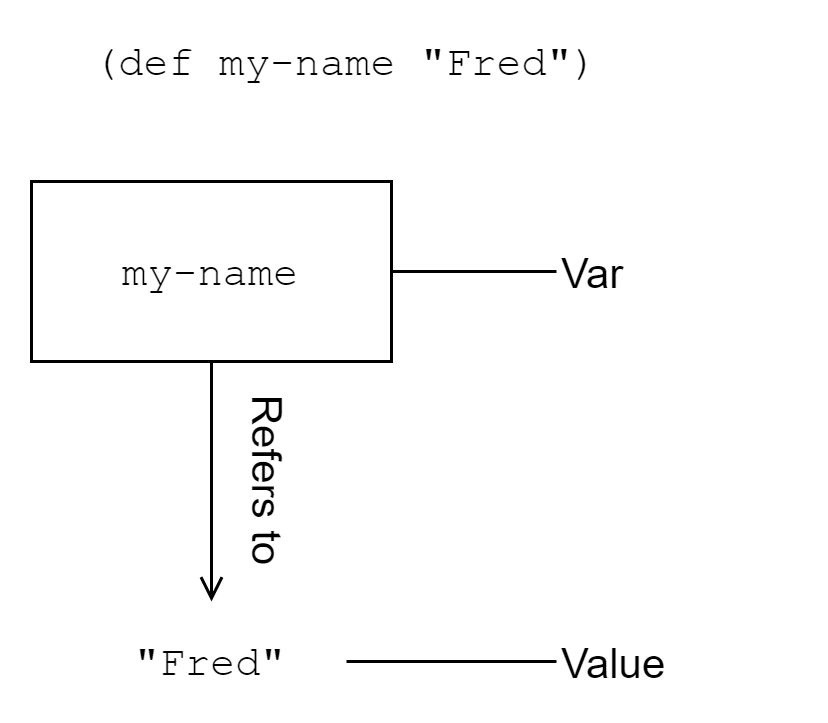
\includegraphics{lesson9/binding-var.png}
\end{figure}

This fictional situation is an analogy to how vars and values work - the
values are the people at the party, and the vars are the name tags. Just
as names may be changed without affecting the people who bear them, vars
may be changed without affecting the values that they name. The process
of associating a var and a value is called \emph{binding}\index{binding} the var to a
value. Please feel free to follow along in the REPL.

\begin{lstlisting}[language=Clojure, caption={Defining vars}]
(def my-name "Fred")                                       %\circled{1}%
;; #'cljs.user/my-name

my-name
;; "Fred"

(defn mk-global [value]
  (def i-am-global value))
;; #'cljs.user/mk-global

mk-global                                                  %\circled{2}%
;; #object[ ... ]

(mk-global [4 8 15 16 23 42])
;; #'cljs.user/i-am-global

i-am-global                                                %\circled{3}%
;; [4 8 15 16 23 42]

(def ten 10)
;; #'cljs.user/ten

(def twenty (* ten 2))                                     %\circled{4}%
;; #'cljs.user/twenty

twenty
;; 20

ten                                                        %\circled{5}%
;; 10
\end{lstlisting}

\begin{enumerate}[label=\protect\circled{\arabic*}]
\tightlist
\item
  Binding the var, \texttt{my-name} to the value \texttt{"Fred"}
\item
  \texttt{defn} created a function and bound it to the var,
  \texttt{mk-global}
\item
  Even though the \texttt{i-am-global} var was defined \emph{inside} the
  \texttt{mk-global} function, it is global to the \texttt{cljs.user}
  namespace
\item
  Since expressions evaluate to values, \texttt{twenty} gets bound to
  the result of \texttt{(*\ ten\ 2)}, or \texttt{20}
\item
  We verify that the value of ten was not changed when we multiplied it
  by 2
\end{enumerate}


\subsection{Symbols}

\index{data types!symbols}In Lesson 3, we looked very briefly at symbols, which are essentially
names that refer to something else, usually a var. In the REPL session
above, \texttt{my-name}, \texttt{mk-global}, \texttt{i-am-global},
\texttt{ten}, and \texttt{twenty} are all symbols. That is, they are
names that refer to the var that we have bound. When ClojureScript is
evaluating our program code and comes across a symbol, it will try to
evaluate the symbol to whatever it refers to, and if it cannot resolve
the symbol to any known value, it will display a warning.

\begin{lstlisting}[language=Clojure, caption={Symbols}]
(def x 7)                                                  %\circled{1}%
;; #'cljs.user/x

x                                                          %\circled{2}%
;; 7

'x                                                         %\circled{3}%
;; x

(defn doubler [x] (* 2 x))                                 %\circled{4}%
;; #'cljs.user/doubler

(doubler 3)
;; 6

y                                                          %\circled{5}%
;; WARNING: Use of undeclared Var cljs.user/y at line 1 <cljs repl>
;; nil
\end{lstlisting}

\begin{enumerate}[label=\protect\circled{\arabic*}]
\tightlist
\item
  Use the symbol \texttt{x} to refer to a var
\item
  The symbol evaluates to the thing it refers to
\item
  A quote before the symbol causes ClojureScript to evaluate the symbol
  \emph{itself}, not the thing it refers to
\item
  Within the function, the symbol \texttt{x} refers to the function
  parameter, not the global var
\item
  Warning when trying to evaluate a symbol that does not refer to
  anything
\end{enumerate}


\begin{notice}[title={You Already Know How to Use It}]
In JavaScript, we already work with immutable data on a daily basis.
Strings and numbers in JavaScript are immutable - they are values that
can not be changed. We can \emph{derive} new values from them, but we
(thankfully) can't say that \texttt{1\ =\ 2} or
\texttt{"Unchangeable"\ +=\ "...\ or\ not"}. It is perfectly natural for
us to think about these sorts of values as immutable, but we have a more
difficult time thinking about collections as immutable. More seasoned
programmers who have encountered immutable data structures may tend to
think of them as ``bulky'' or resource-intensive (and many
implementations of them are indeed inefficient). Whether we are simply
used to mutable collections from other languages or have a notion of
immutable collections as being impractical, it takes a while to get into
the habit of working with immutable collections However, once we get
used to it, thinking of maps, vectors, et al.~as values becomes as
natural as thinking about strings and numbers in the same way.
\end{notice}

\subsection{You Try It}

Almost everything in ClojureScript is a value, and a var can be bound to
any value. With this knowledge, use \texttt{def} to create a var that
refers to this function:

\begin{lstlisting}[language=Clojure]
(fn [message]
  (js/alert (.toUpperCase (str message "!!!!!!!!!!!!!!!!"))))
\end{lstlisting}

Can you use the var that you created to call this function? E.g.
\texttt{(my-var\ "inconceivable")}

\section{Creating Local Bindings With let}

\index{def@\texttt{def}}While \texttt{def} creates a var that is visible to an entire namespace,
we sometimes want to name and use values that are more temporary or
focused in scope. ClojureScript uses \index{let@\texttt{let}}\texttt{let} to create these local
bindings. Like vars, \texttt{let} maps a name to some value, but they do
not stick around after the contents of the \texttt{let} are evaluated.
This can be useful for when we want to name things for convenience in
the middle of a function without polluting the namespace with a bunch of
unnecessary vars. The form of a \texttt{let} expression is as follows:

\begin{lstlisting}[language=Clojure, caption={Let expression}]
(let [bindings]
  expr1
  expr2
  ...
  expr-n)
\end{lstlisting}

\texttt{bindings} are pairs of names and values, such as
\texttt{{[}a\ 20,\ b\ 10,\ c\ (+\ a\ b){]}}, and the entire \texttt{let}
expression evaluates to the value of the last expression inside the body
of the \texttt{let}. Since only the value of the last expression is
considered, the other expressions are only used for side effects,\index{side effects!within let@within \texttt{let}} such
as printing to the console or doing DOM manipulation. Here is an example
of how we might use \texttt{let} in a real application:

\begin{lstlisting}[language=Clojure, caption={Using let}]
(defn parse-msg [msg-raw]
  (let [msg-types {:c ::control
                   :e ::event
                   :x ::error}
        msg (reader/read-string msg-raw)
        type (:t msg)
        data (:d msg)]
    (println "Got data:" data)
    [(get msg-types type) data]))
\end{lstlisting}

There are a couple of important things to notice here. First, the names
that we created with the \texttt{let} - \texttt{msg-types},
\texttt{msg}, \texttt{type}, and \texttt{data} - are only defined for
code inside the \texttt{let} and will be garbage collected\index{garbage collection} when the
\texttt{let} completes evaluation. Second, the names that we declare
first are available in later bindings. For example, we defined
\texttt{msg} as the result of evaluating the expression,
\texttt{(reader/read-string\ msg-raw)}, and then we defined
\texttt{type} and \texttt{data} in terms of \texttt{msg}. This is
perfectly normal and allows us to write much clearer and more concise
code.

\subsection{Quick Review}

\begin{itemize}
\tightlist
\item
  What happens when \texttt{let} creates a binding with the same name as
  a var that is already defined? What will be the output of the
  following code?
\end{itemize}

\begin{lstlisting}[language=Clojure]
(def name "Napoleon")

(let [name "Pedro"]
  (println "Vote 4" name))
\end{lstlisting}

\begin{itemize}
\tightlist
\item
  Fill in the following function so that it tells you the name of your
  favorite dessert:
\end{itemize}

\begin{lstlisting}[language=Clojure]
(let [desserts ["Apple Pie" "Ice Cream Sandwiches" "Chocolates" "Berry Buckle"]
      favorite-index 1
      favorite-dessert (get desserts favorite-index)]
  (println "All desserts are great, but I like" favorite-dessert "the best"))
\end{lstlisting}

\subsection{Destructuring Bindings}

\index{destructuring}The \texttt{let} form allows us to do more than bind a single name at a
time. We can use it to assign names to elements in a list or vector as
well as entries in a map. In the simplest case, we can declare a vector
of names on the left-hand side of the binding and a sequence on the
right-hand side. The nth name in the vector will be bound to the nth
element in the sequence on the right (or \texttt{nil} if no such element
exists):

\begin{lstlisting}[language=Clojure, caption={Vector bindings}]
(let [[id name rank extra] [420 "Pepper" "Sgt."]]
  (println "Hello," rank name "- you have ID =" id "and extra =" extra))

;; Hello, Sgt. Pepper - you have ID = 420 and extra = nil
\end{lstlisting}

If we are not interested in assigning a name of a particular element, we
can use an \texttt{\_} as its name, as in the following example:

\begin{lstlisting}[language=Clojure, caption={Discarding a value}]
(let [[_ name rank] [420 "Pepper" "Sgt."]]
  (println "Hello," rank name))

;; Hello, Sgt. Pepper
\end{lstlisting}

Another common case is assigning some trailing portion of a sequence to
a name. This can be done by inserting a \texttt{\&\ other} at then end
of the binding:

\begin{lstlisting}[language=Clojure, caption={Rest bindings}]
(let [[eat-now & eat-later] ["nachos" "salad" "apples" "yogurt"]]
  (println "Please pass the" eat-now)
  (println "I'm saving these for later:" eat-later))

;; Please pass the nachos
;; I'm saving these for later: (salad apples yogurt)
\end{lstlisting}

In addition to destructuring lists and vectors, we can also destructure
maps by providing a map on the left-hand side of the binding whose keys
are the names to which the properties should be bound and whose values
are the keys in the map on the right-hand side to bind:

\begin{lstlisting}[language=Clojure, caption={Map bindings}]
(let [{x :x
       y :y} {:x 534 :y 497 :z -73}]
  (println "Inspecting coordinates:" x "," y))

;; Inspecting coordinates: 534 , 497
\end{lstlisting}

However, since we often work with maps of keywords, there is a more
succinct way to bind specific values from a map to names that are
similar to their key:

\begin{lstlisting}[language=Clojure, caption={Binding keys}]
(let [{:keys [x y z]} {:x 534 :y 497 :z -73}]
  (println "x = " x "| y = " y "| z = " z))

;; x =  534 | y =  497 | z =  -73
\end{lstlisting}

For maps with string keys there is a similar syntax that uses
\texttt{:strs} instead of \texttt{:keys} in the binding.

Finally, when destructuring maps, we may provide default values using
\texttt{:or} inside the binding form followed by a map of name to
default value:

\begin{lstlisting}[language=Clojure, caption={Default values}]
(let [{:keys [fname lname profession]
       :or {profession "professional"}} {:fname "Sasha" :lname "Simonova"}]
  (println fname lname "is a" profession))

;; Sasha Simonova is a professional
\end{lstlisting}

There are more variations to ClojureScript's destructuring
forms\footnote{The official Destructuring in Clojure guide - located at https://clojure.org/guides/destructuring - is an excellent reference}, but we have covered the
most common ones that we will use for the rest of this book.

\subsection{You Try It}

\begin{itemize}
\tightlist
\item
  What happens when you use the \texttt{\&\ other} form when there are
  no more elements in a list/vector?
\end{itemize}

\begin{verbatim}
(let [[one two & the-rest] [1 2]]
  the-rest)
\end{verbatim}

\section{Summary}

We have now gone over the two primary means of naming things in
ClojureScript \texttt{def} for namespace-level bindings and \texttt{let}
for local bindings - so we are ready to tackle one of ``the only two
hard problems in computer science''\footnote{Did you catch the
  reference to Phil Karlton's famous quote, ``There are only two hard
  things in Computer Science: cache invalidation and naming things.''}.
Combining this knowledge with what we will learn in the next few
lessons, we will be able to start writing some interesting applications.
We can now:

\begin{itemize}
\tightlist
\item
  Explain what a var is and how it is referred to by a symbol
\item
  Define global bindings using \texttt{def}
\item
  Define local bindings using \texttt{let}
\item
  Destructure sequences and maps
\end{itemize}

\chapter{Making Choices}

Up to this point, we have mostly been writing code that has some
starting point and progresses until it is complete.\footnote{We have
  come across some code samples that have used conditionals because they
  are almost unavoidable for any interesting program.} It has a
well-defined task and must follow a well-defined series of instructions
to accomplish this task. What we have been missing is the concept of a
\emph{choice} - being able to take a different path depending on some
condition. Imagine a road that stretched for hundreds and hundreds of
miles without ever intersecting with another road. If we were to drive
along that road, it would be easy because we would never have to decide
whether to take another route; however, the drive would also be fairly
uneventful. It is the same with the code that we write: we could write
scripts that simply run from top to bottom and have a clear linear
execution, but then we would be missing out on the most interesting and
rewarding programs.

\begin{center}\rule{0.5\linewidth}{0.5pt}\end{center}

\textbf{In this lesson:}

\begin{itemize}
\tightlist
\item
  Apply \texttt{if} and \texttt{when} to make simple choices
\item
  Become familiar with the concept of truthiness and how it is defined
\item
  Choose between multiple options with \texttt{cond}
\end{itemize}

\begin{center}\rule{0.5\linewidth}{0.5pt}\end{center}


\section{Example: Adventure Game}

\begin{figure}[H]
\caption{Text-based adventure game}
\centering
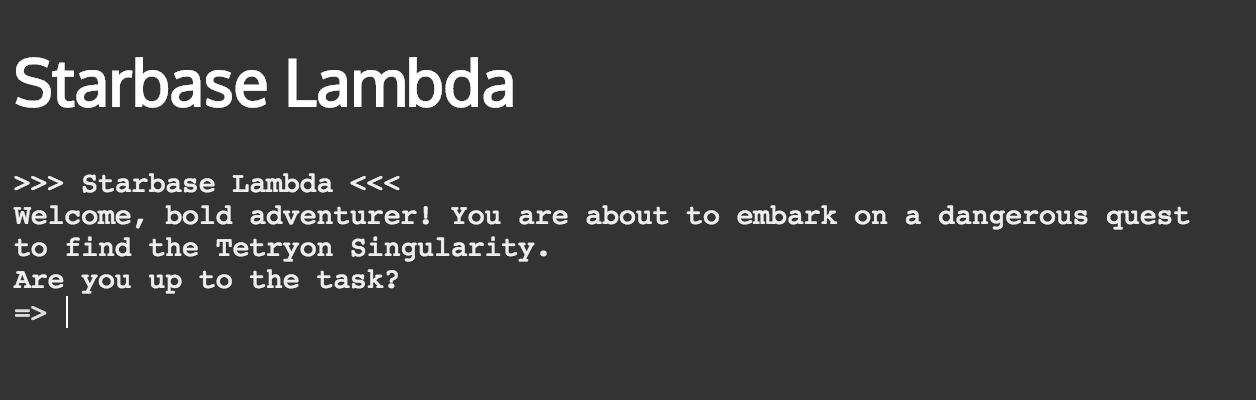
\includegraphics[width=10cm]{lesson10/adventure-screenshot.png}
\end{figure}


In this lesson, we will build a simple text-based adventure game.
Adventure games are perfect for learning the concept of conditionals,
since they are built around letting the user make a series of choices of
how to navigate a virtual environment. So that we can focus on learning
one building block at a time, we will use the author's
\emph{bterm} terminal emulator library\footnote{https://github.com/kendru/bterm}.
This will allow us to focus on the core concepts of control structures
without getting mired in DOM manipulation and event handling or learning
a large framework.

\section{Making Simple Choices With if And when}

When we are making choices, we usually need to determine if something is
true or false: is a particular checkbox selected? Is the account balance
below some threshold? Does the player have some particular potion in
their inventory? These kinds of questions can only have one of 2 answers
- ``yes'' or ``no''. Remember that ClojureScript works by
\emph{evaluating expressions}, so these questions usually take the form
of an expression that evaluates to something that is either true or
false. We could imagine the above questions translated to ClojureScript
expressions:

\begin{lstlisting}[language=Clojure, caption={Expressions that ask questions}]
;; Is the checkbox checked?
(aget my-checkbox "checked")

;; Is the account balance below a threshold?
(< (:balance account) low-balance-threshold)

;; Does the player have the potion of wisdom in their inventory?
(some #(= (:name %\%%) "Potion of Wisdom")
      (get-inventory player))
\end{lstlisting}

When we evaluate one of these expressions (assuming that the vars we
reference are actually defined), the value will be something that we can
consider to be either \emph{true} or \emph{false}.

\subsection{Selecting With if}

\index{conditional expressions!if@\texttt{if}}We often want to make one choice when the answer is true and another
choice when the answer is false - in this situation, we can use
ClojureScript's \texttt{if} special form. An if expression takes the
following form:

\begin{lstlisting}[language=Clojure]
(if test-expr then-expr else-expr)
\end{lstlisting}

\texttt{if} takes 3 expressions: a test, a value to use if the test is
true, and a value to use if the test is false. The entire \texttt{if}
expression will evaluate to the value of either the second or third
expression depending on the value of the first expression. To use the
account balance example from above, we could write the following:


\begin{lstlisting}[language=Clojure]
(def account-status
  (if (< (:balance account) low-balance-threshold)         %\circled{1}%
    :low-balance                                           %\circled{2}%
    :ok))                                                  %\circled{3}%
\end{lstlisting}

\begin{enumerate}[label=\protect\circled{\arabic*}]
\tightlist
\item
  Test whether the balance is below some point
\item
  If the test is true, evaluate to \texttt{:low-balance}
\item
  If the test is false, evaluate to \texttt{:ok}
\end{enumerate}

\begin{notice}[title={Special Forms}]
When we write an s-expression, ClojureScript will evaluate it as long as
the first symbol in the expression resolves to the name of a function, a
macro, or a \emph{special form}. While the call to \texttt{if} looks
just like a function call, \texttt{if} is actually a special form rather
than a function. We have now been writing functions for a while, and we
will learn to write macros in a later lesson, but special forms are
baked into the language because they are so fundamental that they cannot
be implemented as a library function (or at least not efficiently).
Thankfully, from our perspective as developers, we do not need to be
concerned whether the specific thing that we are calling is a function,
macro, or special form, since there is no difference in the way that
they are called.
\end{notice}

While the idea of an \texttt{if} statement should be familiar to any
developer, there is a key difference between most languages' if
statement and ClojureScript's if: in ClojureScript, \texttt{if} is an
expression, so it always evaluates to a specific value. In an imperative
language like JavaScript, the \texttt{if} statement usually makes a
choice between which code branch to \emph{execute}. The actual if
statement does not yield a value. For instance, the following is not
valid JavaScript:

\begin{lstlisting}[language=JavaScript, caption={JavaScript ifs are not expressions}]
// This will throw a SyntaxError
const answer = if (someCondition) {
   'Yes';
} else {
   'No';
}
\end{lstlisting}

However, JavaScript does provide the ternary operator\index{ternary operator}, which is an
expression. ClojureScript's \texttt{if} expression is very similar to
JavaScript's ternary operator, but there is one less piece of syntax to
deal with!

\begin{lstlisting}[language=JavaScript, caption={\ldots{}but ternaries are}]
const answer = someCondition ? 'Yes' : 'No';
\end{lstlisting}

In JavaScript - as in most imperative languages - we use \texttt{if}
statements to perform side effects such as conditionally setting a
variable, prompting the user for input, or manipulating the DOM. In
ClojureScript, we usually use the \texttt{if} expression to decide
between two values. The entire expression will take the value of either
the \texttt{then} expression or the \texttt{else} expression. Selecting
between more than 2 values can also be accomplished by replacing either
the \texttt{then} or \texttt{else} expression with another (nested)
\texttt{if} expression.

\begin{figure}[H]
\caption{Conditional evaluation}
\centering
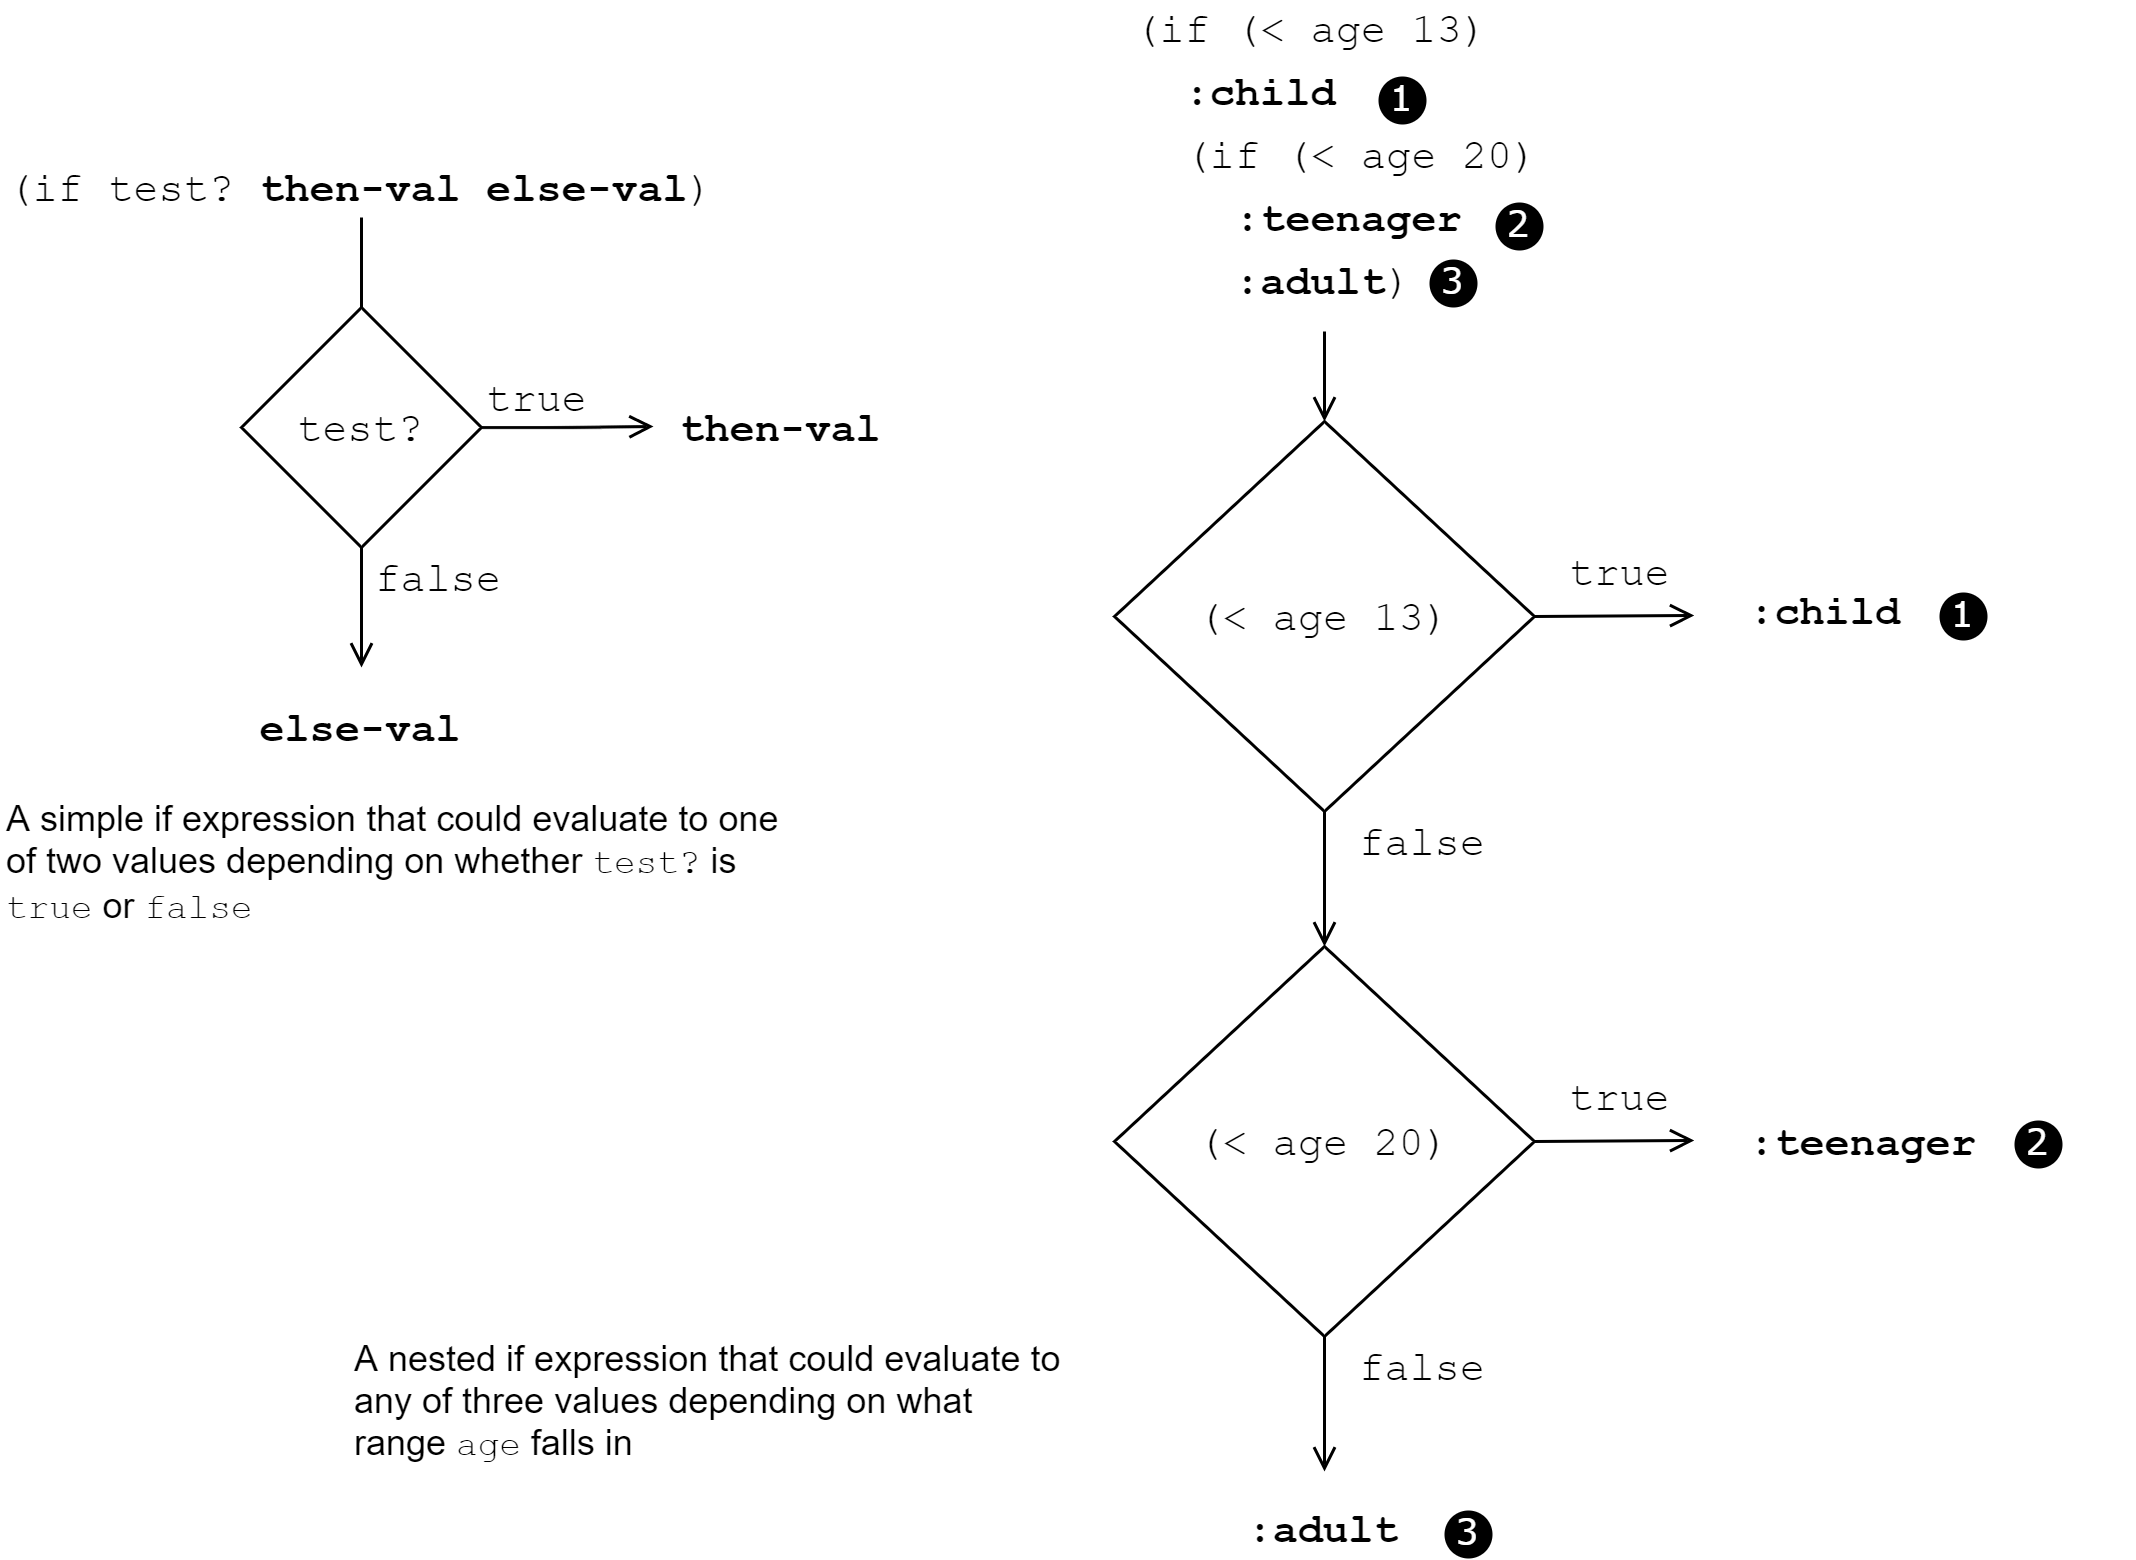
\includegraphics[width=12cm]{lesson10/selecting-expressions.png}
\end{figure}

Take care, however, as deeply nested if expressions can be difficult to
read and can usually be replaced with a \texttt{cond}, which we will
learn about later in this lesson.

\subsection{Quick Review}

\begin{itemize}
\tightlist
\item
  Explain the difference between \texttt{if} in JavaScript and
  ClojureScript
\item
  How would you write an \texttt{if} expression that - given 2 numeric
  values, \texttt{a} and \texttt{b} - would evaluate to
  \texttt{"greater"} if a \textgreater{} b, \texttt{"less"} if a
  \textless{} b, or \texttt{"same"} if they are equal?
\end{itemize}


\subsection{Conditional Evaluation With when}

\index{conditional expressions!when@\texttt{when}}Closely related to \texttt{if} is the \texttt{when} expression. We can
think of it as an \texttt{if} without an \texttt{else} expression:

\begin{lstlisting}[language=Clojure]
(when test-expr some-value)
\end{lstlisting}

When the test expression is true, the entire expression evaluates to the
value given, and when the test is false, the expression evaluates to
\texttt{nil}. In fact, \texttt{when} is just shorthand for an
\texttt{if} where the \texttt{else} expression is \texttt{nil}:

\begin{lstlisting}[language=Clojure]
(if test-expr some-value nil)
\end{lstlisting}

The two common use cases for \texttt{when} are to transform a value only
when it is non-nil and to perform some side effect when a certain
condition holds true. For the first case, we often see code like the
following:

\begin{lstlisting}[language=Clojure, caption={Operate on non-nil values}]
(defn conversion-rate [sessions]                           %\circled{1}%
  (let [users (user-count sessions)
        purchases (purchase-count sessions)]
    (when (> users 0)                                      %\circled{2}%
      (/ purchases users))))
\end{lstlisting}

\begin{enumerate}[label=\protect\circled{\arabic*}]
\tightlist
\item
  Define a function that gets the ratio of purchases to users
\item
  Use \texttt{when} to prevent division by zero
\end{enumerate}

\index{side effects!within when@within \texttt{when}}For the second case, we will often want to perform some DOM manipulation
or other side effect only in a specific case. For instance, we may want
to pop up an error message when we receive a server error from a
back-end API:

\begin{lstlisting}[language=Clojure, caption={Conditionally perform side effect}]
(when (< 499 (:status response))
  (show-error-notification (:body response)))
\end{lstlisting}

\subsection{Applying if and when}

Considering the example of the adventure game, we can use use an
\texttt{if} expression to determine what to do after prompting the user
for a yes/no question. Let's take a quick step back to discuss the
overall architecture of the game. We will represent the entire game as a
map where the keys are the name of each state and the values are maps
that represent a specific screen. The general shape of our game data
structure is below:

We will represent our game as a collection of states with rules that
determine how to move between states when the user makes some decision:

\begin{lstlisting}[language=Clojure, caption={Game states}]
{:start { ... }
 :state-1 { ... }
 :state-2 { ... }
 :state-3 { ... }
 :win { ... }}
\end{lstlisting}

Our game will start with the user in a spaceship at Starbase Lambda,\index{Starbase Lambda} and
their goal is to uncover the location of the \textbf{Tetryon
Singularity}. They will issue simple commands as well as answer ``yes''
or ``no'' questions.

Each state in the game (which we filled in with \texttt{\{\ ...\ \}}
above) will contain a \texttt{:type}, \texttt{:title}, \texttt{:dialog},
and \texttt{:transitions}. The type determines what sort of state the
game is in - e.g.~\texttt{:start}, \texttt{:win}, or \texttt{:lose} -
title and dialog determine what we display onscreen, and the transitions
determine which state the user should transition to depending on the
choice that they make. For example:

\begin{lstlisting}[language=Clojure, caption={Example game state}]
{:type :start
 :title "Starbase Lambda"
 :dialog (str "Welcome, bold adventurer! You are about to embark on a dangerous "
              "quest to find the Tetryon Singularity.\nAre you up to the task?")
 :transitions {"yes" :embarked,
               "no" :lost-game}}
\end{lstlisting}

When the user is in this state, we will print the title and dialog to
the screen and prompt them for input. If they type ``yes'', we'll
advance to the \texttt{:embarked} state; otherwise, we'll move on to the
\texttt{:lost-game} state.

Instead of walking through scaffolding a new project, we can checkout a
skeleton project from the book's GitHub repo, which already has the
necessary dependencies configured in \texttt{deps.edn} as well as some
basic markup and styles. We will be working from Git tag
\texttt{lesson10.1}.

\subsection{Prompting for Input}

The first thing that we will want to do is display the title and dialog
from whatever scene the user is currently in and prompt them for input.
We'll handle the input later, so for now let's just think about how we
can display the scene. The bterm library that we are using provides
several useful functions for controlling output:

\begin{itemize}
\tightlist
\item
  \texttt{print} - prints a screen to the terminal
\item
  \texttt{println} - prints a screen to the terminal with a trailing
  newline character
\item
  \texttt{clear} - clears any existing output from the terminal
\end{itemize}

With this in mind, let's think about how to display the scene. We always
want to print the title and dialog, but we should also indicate if they
have won or lost the game. In this case, we can display either, ``You've
Won!'' or ``Game Over''. To accomplish this, we can first test the type
of the current scene and only display the end game message if the type
is either \texttt{:win} or \texttt{:lose}:

\begin{lstlisting}[language=Clojure, caption={Checking for game end}]
(when (or (= :win type)                                    %\circled{1}%
          (= :lose type))
  ;; Display message                                       %\circled{2}%
  )
\end{lstlisting}

\begin{enumerate}[label=\protect\circled{\arabic*}]
\tightlist
\item
  Check if user is in an end-game state
\item
  Perform the side effect of printing some message
\end{enumerate}

Furthermore, we want to use a different message depending on whether the
user has won or lost. We can accomplish this with \texttt{if}:

\begin{lstlisting}[language=Clojure]
(io/println term
            (if (= :win type) "You've Won!" "Game Over"))
\end{lstlisting}

The \texttt{if} expression will evaluate to either ``You've Won!'' or ``Game Over'' depending on the value of \texttt{type}.

Putting these pieces together with the printing of the title and dialog
gives us something like this:

\begin{lstlisting}[language=Clojure, caption={Prompting for input}]
(defn prompt [game current]                                %\circled{1}%
  (let [scene (get game current)                           %\circled{2}%
        type (:type scene)]
    (io/clear term)
    (when (or (= :win type)                                %\circled{3}%
              (= :lose type))
      (io/print term
                (if (= :win type)                          %\circled{4}%
                    "You've Won! "
                    "Game Over ")))
    (io/println term (:title scene))                       %\circled{5}%
    (io/println term (:dialog scene))
    (io/read term #(on-answer game current %\%%))))        %\circled{6}%
\end{lstlisting}

\begin{enumerate}[label=\protect\circled{\arabic*}]
\tightlist
\item
  This function takes the entire game data structure and the current
  scene
\item
  Create 2 local bindings with \texttt{let} that we will use in the rest
  of the function
\item
  Conditionally print an end-game message
\item
  Determine which message to print
\item
  Print the title and dialog no matter what the scene type is
\item
  Handle whatever the user types using the on-answer function that we
  are about to write
\end{enumerate}

\subsection{Handling Input}

Now that we have taken care of the display side of things, we will want
to handle user input. In the previous snippet, we passed control to the
\texttt{on-answer} function when the user entered an answer. This
function, like \texttt{prompt}, is passed the entire game data structure
as well as the key identifying the current scene; however, it is also
passed the string that the user entered at the prompt. Using this
information, we need to determine which scene to display next then
prompt the user for input once more. Here is the skeleton of what this
code should look like:

\begin{lstlisting}[language=Clojure]
(defn on-answer [game current answer]
  (let [scene (get game current)
        next ;; TODO: determine the next state
        ]
    (prompt game next)))
\end{lstlisting}

To start, we only need to handle responses of ``yes'' or ``no''. Since
we are only deciding between 2 options, a single \texttt{if} expression
will suffice:

\begin{lstlisting}[language=Clojure]
(if (= "yes" answer)
  (get-in scene [:transitions "yes"])
  (get-in scene [:transitions "no"]))
\end{lstlisting}

\subsection{You Try It}

There is another type of game state that we need to handle =
\texttt{:skip}, which has the following shape:

\begin{lstlisting}[language=Clojure]
{:type :skip
 :title "..."
 :dialog "..."
 :on-continue :next-state}
\end{lstlisting}

Add another conditional to the \texttt{on-answer} function that will
proceed to the next state regardless of what the user enters. A possible
solution is given below:

\begin{lstlisting}[language=Clojure]
(defn on-answer [game current answer]
  (let [scene (get game current)
        next (if (= :skip (:type scene))
               (:on-continue scene)
               (if (= "yes" answer)
                 (get-in scene [:transitions "yes"])
                 (get-in scene [:transitions "no"])))]
    (prompt game next)))
\end{lstlisting}

\section{Truthiness and Falsiness}

\index{truthiness}Before continuing, let's take a brief step back to talk about the
concept of truthiness in ClojureScript. The test expression that we pass
to \texttt{if} or \texttt{when} can be an actual boolean value -
\texttt{true} or \texttt{false} - but it does not have to be. As in
JavaScript, we can pass any value as the test. Even if it is not a
boolean, the language will either consider it to be ``truthy'' and pass
the test or ``falsy'' and fail it.

Unlike JavaScript, which has a number of special cases that it considers
to be falsey, ClojureScript follows a very simple rule: \texttt{false}
and \texttt{nil} are falsy, and \emph{everything else} is truthy.

\begin{notice}[title={ClojureScript's Truthiness Rule}]
\texttt{false} and \texttt{nil} are falsy, and all other values are truthy.
\end{notice}

\subsection{Quick Review}

\begin{itemize}
\tightlist
\item
  What is the value of \texttt{(if\ TEST\ "Truthy"\ "Falsy")} for each
  of the following values for ``TEST'':

  \begin{itemize}
  \tightlist
  \item
    \texttt{true}
  \item
    \texttt{false}
  \item
    \texttt{"false"}
  \item
    \texttt{""}
  \item
    \texttt{0}
  \item
    \texttt{nil}
  \item
    \texttt{js/NaN}
  \item
    \texttt{{[}{]}}
  \end{itemize}
\end{itemize}

\section{More Complex Choices With cond}

With \texttt{if} and \texttt{when}, we have all that we technically need
to handle any sort of decision-making that we need to do in code.
However, we are often faced with cases in which \texttt{if} would be
awkward to use. Consider adding more commands to our game so that the
user could type ``restart'' to go back to the beginning or ``help'' to
display the commands that are available. As we add more options, we
would have to keep nesting more and more\texttt{if} expressions - like
using a pocket knife to carve a wooden sculpture, it could work, but the
result would not be pleasant.

\index{conditional expressions!cond@\texttt{cond}}Enter \texttt{cond} and its cousins, \texttt{condp} and \texttt{case}.
\texttt{cond} takes some expression and any number of test/result pairs,
and the entire expression will evaluate to the ``then'' expression that
comes after the first test that is truthy:

\begin{lstlisting}[language=Clojure, caption={The structure of \texttt{cond}}]
(cond
  test-1 then-1
  test-2 then-2
  ;; ...
  test-n then-n)
\end{lstlisting}

It is idiomatic to use \texttt{:else} as the test expression for a
``fall-through'' value if no other test is truthy. Remember that only
\texttt{false} and \texttt{nil} are falsy, so the keyword \texttt{:else}
will always be truthy and will satisfy \texttt{cond} if no prior test
does. Thinking about the additional commands that we would like to add
to our game, this would be much simpler using cond.

\begin{figure}[H]
\caption{Replacing nested if with cond}
\centering
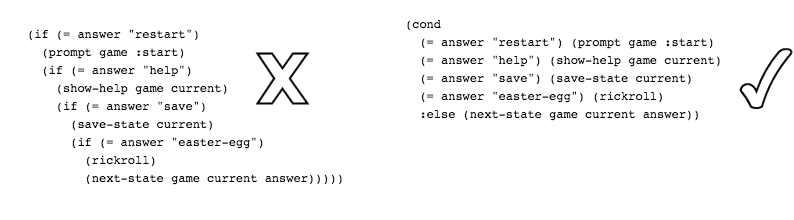
\includegraphics[width=12cm]{lesson10/cond-if-comparison.png}
\end{figure}

\subsection{Repeated Tests With condp}

\index{conditional expressions!condp@\texttt{condp}}If this was as good as we can do, it would be a significant improvement,
but we can still simplify things further with a more focused variation
of \texttt{cond} called \texttt{condp}. Like \texttt{cond},
\texttt{condp} allows us to choose from among a number of options, but
if there is a lot of common code in each of the test expressions,
\texttt{condp} can usually help us factor it out. In our case, we test
the value of ``answer'' for equality with some string in every test
expression.

This is a great case for \texttt{condp}, which takes 1) a binary
predicate -- that is, a function that take two arguments and returns a
boolean value, e.g.~\texttt{=} 2) an expression to use as the right-hand
side in every test, and 3) any number of left-hand
test-expression/result pairs. It can also take 4) an optional default
value to use if none of the prior tests were truthy.

\begin{lstlisting}[language=Clojure, caption={The structure of \texttt{condp}}]
(condp pred expr
  test-expr-1 then-1
  test-expr-2 then-2
  ;; ...
  test-expr-n then-n
  default-expr)
\end{lstlisting}

For every test expression/result pair, it applies the predicate to the
test expression and the other expression and evaluates to the first
result value whose test expression passed the predicate. On paper, this
can be confusing, but seeing an example can help clarify things, so here
is our text-based menu re-written using \texttt{condp}:

\begin{lstlisting}[language=Clojure, caption={Menu refactored with condp}]
(condp
  =                                                        %\circled{1}%
  answer                                                   %\circled{2}%
  "restart" (prompt game :start)                           %\circled{3}%
  "help" (show-help game current)
  "save" (save-state current)
  "easter-egg" (rickroll)
  (next-state game current answer))                        %\circled{4}%
\end{lstlisting}

\begin{enumerate}[label=\protect\circled{\arabic*}]
\tightlist
\item
  Use the \texttt{=} predicate function to test each option
\item
  Pass \texttt{answer} as the right-hand side in every test
\item
  Each clause will be tested as \texttt{(=\ "restart"\ answer)}
\item
  Provide a default expression if every prior test fails
\end{enumerate}

Compared to our original implementation with nested if statements, this
version using \texttt{condp} is quite succinct and readable. For this
reason, condp is widely used to test multiple values when the full
flexibility of case is not required.


\subsection{Quick Review}

\begin{itemize}
\tightlist
\item
  Using \texttt{cond} to write some code that will evaluate to
  \texttt{:pos} when a given number is positive, \texttt{:neg} when it
  is negative, and \texttt{:zero} when it is exactly zero
\item
  Write code that will do the same thing using \texttt{condp}
\end{itemize}


\section{Summary}

In this lesson, we learned what are usually referred to as the branching
control structures. We learned that, in contrast to JavaScript and other
imperative languages, these structures are used as expressions that
choose between values rather than imperative statements that direct the
flow of execution. We also looked at ClojureScript's concept of
truthiness and how it is simpler than that of most other languages. We
can now:

\begin{itemize}
\tightlist
\item
  Choose between two values using \texttt{if}
\item
  Conditionally evaluate code using \texttt{when}
\item
  Simplify multiple-choice options using \texttt{cond} and
  \texttt{condp}
\end{itemize}

Even though they function a little differently in ClojureScript than in
other languages, these branching mechanisms are one of the most
fundamental building blocks that we need to write applications. Next, we
will look at the other class of control structures - loops.

\chapter{Looping}

In the last lesson, we looked at ClojureScript's versions of we usually
call branching control structure. However, we learned that things work a
little bit different in ClojureScript compared to other languages that
we may be used to - control structures are expressions rather than
imperative controls. Now as we come to another fundamental topic - loops
- we will learn that things are once again a bit different in
ClojureScript.

\begin{center}\rule{0.5\linewidth}{0.5pt}\end{center}

\textbf{In this lesson:}

\begin{itemize}
\tightlist
\item
  Survey ClojureScript's various looping structures
\item
  Learn to think in terms of sequences
\item
  Force evaluation of loops for side effects
\end{itemize}

\begin{center}\rule{0.5\linewidth}{0.5pt}\end{center}

\index{loops}In imperative languages, loops are used to repeat the same instructions
multiple times, usually with some small variation each time that will
eventually cause the loop to exit. The classic imperative loop is a
\texttt{while} loop in which the computer simply executes the same
instructions over and over until some condition is met:

\begin{lstlisting}[language=JavaScript, caption={While loop in JavaScript}]
let i = 0;                                                 %\circled{1}%

while (i < 10) {                                           %\circled{2}%
    console.log("Counting: " + i);
    i++;                                                   %\circled{3}%
}
\end{lstlisting}

\begin{enumerate}[label=\protect\circled{\arabic*}]
\tightlist
\item
  Initialize a variable that will be mutated
\item
  Set the condition for continuing the loop
\item
  Increment the value of \texttt{i} after every pass
\end{enumerate}

Since ClojureScript emphasizes both immutability of data and
expression-oriented programming - and loops are inherently both mutable
and statement-oriented - one must wonder whether there is any place in
ClojureScript for loops. The answer is both ``yes'' and ``no'' - there
are several loop-like constructs, which we will look at momentarily, but
upon closer inspection, they are abstractions for other concepts that do
not involve explicit looping.

\section{Manipulating Sequences with for}

\index{looping constructs!for@\texttt{for}}The first, and perhaps most common, expression that we will study in
this lesson is \texttt{for}. Although it shares a name with a certain
imperative loop, it is a different animal altogether. In contrast to the
iterative \texttt{for}, ClojureScript's \texttt{for} is centered around
the idea of a sequence comprehension\index{sequence comprehension}, in which we create a new sequence
by transforming, and optionally filtering, an existing one. There are
multiple ways to accomplish this task in ClojureScript, but \texttt{for}
is certainly a concise and idiomatic option.

In its most basic form, \texttt{for} takes any number of sequences and a
body, and it yields a new sequence by evaluating the body for every
combination of sequence elements:

\begin{lstlisting}[language=Clojure, caption={\texttt{for} dissected}]
(for [elem1 sequence1                                      %\circled{1}%
      elem2 sequence2]                                     %\circled{2}%
  expr)                                                    %\circled{3}%
\end{lstlisting}

\begin{enumerate}[label=\protect\circled{\arabic*}]
\tightlist
\item
  Bind each element from \texttt{sequence1} in turn to \texttt{elem1}
\item
  Do the same for \texttt{sequence2}
\item
  For every combination of elements from \texttt{sequence1} and
  \texttt{sequence2}, evaluate \texttt{expr} with the bindings,
  \texttt{elem1} and \texttt{elem2}
\end{enumerate}

\subsection{Using for With a Single Sequence}

Although \texttt{for} supports an arbitrary number of sequences, in
practice it is most commonly used with just one or two. The most common
usage is - as we have already mentioned - as a sequence transformation.
Say we have a list of numbers and we want to find the square of each of
them. What we want is to somehow describe a process that yields a new
list in which each element is the square of the corresponding element in
the original list. Thankfully, this is even easier to express in code
than in words:

\begin{lstlisting}[language=Clojure, caption={Finding the square of 0-9}]
(for [n (range 10)]                                        %\circled{1}%
  (* n n))                                                 %\circled{2}%
;; (0 1 4 9 16 25 36 49 64 81)
\end{lstlisting}

\begin{enumerate}[label=\protect\circled{\arabic*}]
\tightlist
\item
  Yield a new sequence by taking the numbers 0-9
\item
  Make each number in the new sequence the square of the original
\end{enumerate}

By now we should see that when used with a single input sequence,
\texttt{for} describes a whole-sequence transformation. When working
with ClojureScript, we should try to think whether the problem before us
could be represented as a sequence transformation. If so, \texttt{for}
provides a no-nonsense solution. Let's look at the same problem solved
iteratively and with \texttt{for}. Imagine that we have a number of
right triangles. We know the sides that are adjacent to the right angle,
and we need to find the hypotenuse of each triangle. Fist, an iterative
solution in JavaScript:

\begin{lstlisting}[language=JavaScript, caption={Get hypotenuse length iteratively}]
let sides = [[4.2, 6], [4, 4], [3, 4], [5.5, 3]];          %\circled{1}%
let lengths = [];                                          %\circled{2}%
let i;

for (i = 0; i < sides.length; i++) {                       %\circled{3}%
    lengths.push(
        Math.sqrt(
                Math.pow(sides[i][0], 2) +
                Math.pow(sides[i][1], 2)
        )
    );
}
\end{lstlisting}

\begin{enumerate}[label=\protect\circled{\arabic*}]
\tightlist
\item
  Model the triangle sides as a 2-dimensional array
\item
  Declare an array to hold the resulting lengths
\item
  Iterate over the elements in sides, pushing the calculated hypotenuse
  length into the \texttt{lengths} array every time
\end{enumerate}

This is pretty straightforward iterative code, but it is still
lower-level than we would like in ClojureScript. With loops like this,
it is easy to get indices mixed up (e.g.~\texttt{sides{[}i{]}{[}0{]}}
versus \texttt{sides{[}0{]}{[}i{]}}) or introduce off-by-1 errors. It is
easy to see that this problem is just transforming one sequence into
another, so we can easily use \texttt{for}:

\begin{lstlisting}[language=Clojure, caption={Get hypotenuse length with \texttt{for}}]
(let [sides-list (list [4.2 6] [4 4] [3 4] [5.5 3])]       %\circled{1}%
  (for [sides sides-list]                                  %\circled{2}%
    (Math.sqrt (+ (Math.pow (first sides) 2)               %\circled{3}%
                  (Math.pow (second sides) 2)))))
                                                           %\circled{4}%
;; (7.323933369440222 5.656854249492381 5 6.264982043070834)
\end{lstlisting}

\begin{enumerate}[label=\protect\circled{\arabic*}]
\tightlist
\item
  Declare a list or pairs that each represent 2 sides of a right
  triangle
\item
  Use a for expression to apply a transformation to every pair in the
  list
\item
  Apply the Pythagorean Theorem to find the length of the hypotenuse
\item
  The result is a sequence with the hypotenuse of each triangle
\end{enumerate}


\subsection{Quick Review}

\begin{itemize}
\tightlist
\item
  Given pairs of points as: {[}{[}x, y{]}, {[}x, y{]}{]} coordinates,
  write a \texttt{for} expression that calculates the distance between
  the points. \emph{Hint: This is very similar to the previous example.}
\end{itemize}


\subsection{Using for With Multiple Sequences}

Some of the power of \texttt{for} comes in its ability to combine
elements from multiple sequences. When given multiple sequences, it will
yield an element for every unique combination of single elements from
each input sequence. This type of combination is called the Cartesian
product and is an important concept in mathematical set theory. Imagine
we are writing an e-commerce app, and for any given product, there are
several variations: color, size, and style. We could use \texttt{for} to
get all of the possible product combinations:

\begin{lstlisting}[language=Clojure, caption={Generating product variations with \texttt{for}}]
(let [colors [:magenta :chartreuse :taupe]                 %\circled{1}%
      sizes [:sm :md :lg :xl]
      styles [:budget :plain :fancy]]
  (for [color colors                                       %\circled{2}%
        size sizes
        style styles]
    [color size style]))                                   %\circled{3}%
;; ([:magenta :sm :plain] [:magenta :sm :regular] [:magenta :sm :fancy]
;; ... [:taupe :xl :plain] [:taupe :xl :regular] [:taupe :xl :fancy])
\end{lstlisting}

\begin{enumerate}[label=\protect\circled{\arabic*}]
\tightlist
\item
  Declare 3 sequences
\item
  Take every possible combination of 1 item from each collection
\item
  Yield a vector of each color, size, and style combination
\end{enumerate}

In this example, we did not do anything with the resulting product
combinations other than pack them into a vector of
\texttt{{[}color\ size\ style{]}}, but we could have performed any sort
of transformation we wanted. Consider that to accomplish the same task
using an iterative loop would have required us to write loops nested 3
levels deep!

\subsection{Loop modifiers: let, when, and while}

So far, we have been using only the basic form of \texttt{for} in which
we take every element from one or more sequences. While this works for
many use cases, there are times that we want to filter the results (say,
we don't want to offer fancy products in the small size). Instead of
filtering the list after for generates it, we can build the filtering
logic directly into the \texttt{for} expression itself using the
\texttt{:when} modifier. Again, there are times that we want to
calculate some intermediate value before yielding a result. Instead of
nesting a \texttt{let} expression inside body of the \texttt{for}, we
can use the \texttt{:let} modifier. Finally, if we only want to take
elements up to some cut-off point, we can use the \texttt{:while}
modifier. To illustrate these modifiers, we will use a somewhat
contrived example:

\begin{lstlisting}[language=Clojure, caption={\texttt{for} modifiers}]
(for [n (range 100)                                        %\circled{1}%
      :let [square (* n n)]                                %\circled{2}%
      :when (even? n)                                      %\circled{3}%
      :while (< n 20)]                                     %\circled{4}%
  (str "n is " n " and its square is " square))            %\circled{5}%

;; ("n is 0 and its square is 0"
;; "n is 2 and its square is 4"
;; "n is 4 and its square is 16"
;; ...
;; "n is 18 and its square is 324")
\end{lstlisting}

\begin{enumerate}[label=\protect\circled{\arabic*}]
\tightlist
\item
  Take n from the range of 0-99
\item
  Declare a binding for the symbol \texttt{square} for each iteration as
  the square of n
\item
  Only include values for which n is even
\item
  Only continue until n reaches 20
\end{enumerate}

To use any of these modifiers, we can simply append it to the list of
sequence expressions. None of these modifiers are difficult to
understand, so we will simply outline each of them below briefly before
moving on.

\begin{itemize}
\tightlist
\item
  \textbf{:let} creates any number of bindings within the body of the
  \texttt{for}. It can use any of the symbols that are defined in the
  \texttt{for} expression as well as any other vars in scope. The usage
  is identical to the regular \texttt{let} form.
\item
  \textbf{:when} determines for which inputs to emit a value. It is
  followed by a predicate expression, and it will emit a value if and
  only if the expression is truthy.
\item
  \textbf{:while} is like \texttt{:when}, but it short-circuits the most
  immediate ``group'' when used with multiple input sequences. That is,
  when placed after some sequence expression, it will skip the remaining
  elements in the sequence after which it is placed and continue with
  the combination that is formed by taking the next item in the previous
  sequence and the first item in the sequence after which it is placed.
  To illustrate this behavior, consider how the placement of the while
  clause affects the behavior of the following example:
\end{itemize}

\begin{figure}[H]
\caption{Behavior of \texttt{:while} modifier}
\centering
\includegraphics[width=10cm]{lesson11/while-short-circuit.png}
\end{figure}

\subsection{Quick Review}

\begin{itemize}
\tightlist
\item
  White a \texttt{for} expression that takes 2 values called \texttt{x}
  and \texttt{y} both from \texttt{(range\ 50)} and yields the pairs
  \texttt{{[}x\ y{]}} for all even values of \texttt{x} and odd values
  of \texttt{y} when the product of \texttt{x} and \texttt{y} is less
  than \texttt{100}.
\item
  Go back to the product variations example and use \texttt{:when} to
  filter out all variations that are both \texttt{:magenta} and
  \texttt{:fancy}.
\end{itemize}


\section{Performing Explicit Recursion with loop and recur}

In the next lesson, we will look in more detail at recursive functions -
that is, functions that call themselves. But as a preview, below is a
simple recursive function that uses the Euclidean algorithm
\footnote{https://en.wikipedia.org/wiki/Euclidean\_algorithm} for calculating the greatest common denominator of two
numbers.

\begin{lstlisting}[language=Clojure, caption={A recursive function}]
(defn gcd [x y]                                            %\circled{1}%
  (if (= y 0)
    x
    (gcd y (mod x y))))                                    %\circled{2}%
;; #'cljs.user/gcd
(gcd 90 60)                                                %\circled{3}%
;; 30
\end{lstlisting}

\begin{enumerate}[label=\protect\circled{\arabic*}]
\tightlist
\item
  Define a \texttt{gcd} function using the Euclidean algorithm
\item
  The function calls itself as the last thing it does
\item
  Test the function with inputs \texttt{90} and \texttt{60}
\end{enumerate}

\index{looping constructs!loop/recur@\texttt{loop/recur}}The next loop-like construct that we will look at is the dynamic duo of
\texttt{loop} and \texttt{recur}. We use \texttt{loop}/\texttt{recur} in
cases where we want to use a recursive process but do not need a
separate, named function for it. The general form that we use with
\texttt{loop} is as follows:

\begin{lstlisting}[language=Clojure, caption={\texttt{loop} dissected}]
(loop [name-1 init-value-1                                 %\circled{1}%
       name-2 init-value-2]
  body-exprs                                               %\circled{2}%
  (recur next-value-1 next-value-2))                       %\circled{3}%
\end{lstlisting}

\begin{enumerate}[label=\protect\circled{\arabic*}]
\tightlist
\item
  Pass in any number of bindings along with their value for the first
  pass of the loop
\item
  Any number of body expressions
\item
  Optionally recur to the beginning of the loop, supplying the values
  for each binding during the next iteration
\end{enumerate}

This is the closest construct to an imperative loop that ClojureScript
has to a traditional imperative loop. \footnote{Interestingly,
  \texttt{loop} compiles down to a \texttt{while} loop in JavaScript.}
Translating our \texttt{gcd} function from above into a
\texttt{loop}/\texttt{recur} form is trivial:

\begin{lstlisting}[language=Clojure, caption={Implementing \texttt{gcd} with \texttt{loop}}]
  (defn gcd-loop [a b]
  (loop [x a                                               %\circled{1}%
         y b]
    (if (= y 0)
      x                                                    %\circled{2}%
      (recur y (mod x y)))))                               %\circled{3}%
;; #'cljs.user/gcd-loop
(gcd-loop 90 60)
;; 30
\end{lstlisting}

\begin{enumerate}[label=\protect\circled{\arabic*}]
\tightlist
\item
  Initialize the loop with the function's inputs
\item
  Return \texttt{x} when \texttt{y} is \texttt{0}
\item
  Recur in the case that \texttt{y} is not \texttt{0}
\end{enumerate}

As we see above, we can easily control when the loop exits and when it
recurses by placing the call to \texttt{recur} inside one branch of a
conditional and another value in the other branch. This gives us the
same sort of granularity that we are probably used to with imperative
loops, but with less boilerplate.


\subsection{recur Nuances}

\texttt{loop} is a very useful construct that lets us simplify many
types of recursive functions. However, it cannot replace all recursive
functions, only a particular class known as ``tail recursive''\index{tail recursion}
functions. These particular functions are ones that call themselves as
the very last thing they do (in the ``tail'' position) of the function.
As we mentioned in the last lesson, every time a recursive function
calls itself, it consumes a stack frame,\index{call stack} and if it recurses too deeply,
the JavaScript runtime will stop execution with an error. However,
recursive processes written with \texttt{loop} and \texttt{recur} can
recurse arbitrarily deeply because the ClojureScript compiler is able to
optimize them into an imperative loop. For this reason, \texttt{loop} is
also usually faster than functional recursion.

Because \texttt{loop} only works with tail recursion, we need to be
careful that no evaluation is attempted after a \texttt{recur}.
Thankfully, the ClojureScript compiler warns us if the \texttt{recur} is
not in the tail position, and it will not compile the code until we move
the \texttt{recur}. Below is an example of a proper call to
\texttt{recur} along with an illegal one.

\begin{lstlisting}[language=Clojure, caption={Legal and illegal \texttt{recur}}]
(loop [i 0
      numbers []]
 (if (= i 10)
   numbers
   (recur (inc i) (conj numbers i))))                      %\circled{1}%
;; [0 1 2 3 4 5 6 7 8 9]
(loop [i 7
       fact 1]
  (if (= i 1)
    fact
    (* i (recur (dec i) (* i fact)))))                     %\circled{2}%
;; ----  Could not Analyze  <cljs form>   line:5  column:22  ----
;;
;;   Can't recur here at line 5 <cljs repl>
;;
;;   1  (loop [i 7
;;   2         fact 1]
;;   3    (if (= i 1)
;;   4      fact
;;   5      (* i (recur (dec i) (* i fact)))))
;;               ^---
;;
;; ----  Analysis Error  ----
;; nil
\end{lstlisting}

\begin{enumerate}[label=\protect\circled{\arabic*}]
\tightlist
\item
  It is legal to recur when it is the last thing to be evaluated in a
  loop
\item
  Cannot recur here because we need to multiply by \texttt{i} after
  recurring
\end{enumerate}

So we see that not every recursive function can be translated into a
\texttt{loop}, but if it can, there is a definite performance benefit.
This has been a rather brief introduction to \texttt{loop}, but we will
use it quite often over the course of this book, so we will have ample
opportunity to get more familiar with it.


\section{Looping for Side Effects}

Having covered \texttt{for} for sequence comprehensions and
\texttt{loop}/\texttt{recur} for explicit recursion. There is one
remaining category of looping in ClojureScript: looping for side
effects. \index{side effects!within loops}Recall that a side effect is an effect that our program causes
outside the pure calculations that it performs, such as adding and
removing DOM nodes or sending data to a server-side API.

One of the difficulties with ClojureScript is that many of its sequence
operations (including \texttt{for}) are \emph{lazy}. That is, they do
not produce results until called on to do so. Consider this \texttt{for}
expression:

\begin{lstlisting}[language=Clojure]
(for [i (range 100)]
  (println i))
\end{lstlisting}

If you enter this into the REPL, it will print the numbers 0-99, just as
we would expect. However, if we were to only request a few values from
the sequence generated by the \texttt{for}, we would see a surprising
result:

\begin{lstlisting}[language=Clojure, caption={Lazy evaluation}]
(take 3                                                    %\circled{1}%
  (for [i (range 100)]
    (println i)))
;; 0                                                       %\circled{2}%
;; 1
;; ...
;; 31
;; (nil nil nil)                                           %\circled{3}%
(do (for [i (range 100)]
      (println i))
    (println "Done"))
;; Done
;; nil                                                     %\circled{4}%
\end{lstlisting}

\begin{enumerate}[label=\protect\circled{\arabic*}]
\tightlist
\item
  Only take 3 elements from the sequence given by the \texttt{for}
  expression
\item
  \texttt{println} gets called only 32 times - not 100
\item
  Since \texttt{println} returns \texttt{nil}, the result is a sequence
  filed with \texttt{nil}
\item
  No numbers are printed, since we never need the results of the
  \texttt{for}
\end{enumerate}


The \texttt{for} will only evaluate when the results are required to
complete some other calculation. If some results are needed, then it
will always evaluate at least as many elements as it needs to, but it
may not evaluate the entire sequence. \footnote{At the time of this writing, ClojureScript will evaluate lazy sequences 32 elements at a time, but this is an implementation detail, and you should never rely on it materializing the entire sequence if not necessary.} This laziness is, as we will see
in a later lesson, very useful for some things, but it can cause unexpected
behavior when dealing with side effects, thus the need to force
evaluation.


\subsection{Evaluating an Existing Sequence With dorun}

\index{looping constructs!dorun@\texttt{dorun}}The first and simplest way to ensure that a sequence is fully evaluated
(and thus all side effects that it may cause are run) is to wrap the
sequence in a \texttt{dorun}. When just given a sequence, it will
execute the code necessary to realize every value in succession, and it
returns nil. For example, we could force the numbers to print in the
example above simply by wrapping the \texttt{for} expression with
\texttt{dorun}:

\begin{lstlisting}[language=Clojure, caption={Forcing evaluation of a lazy sequence}]
(do (dorun                                                 %\circled{1}%
      (for [i (range 100)]
        (println i)))
    (println "Done"))
;; 0                                                       %\circled{2}%
;; 1
;; ...
;; 99
;; Done
;; nil
\end{lstlisting}

\begin{enumerate}[label=\protect\circled{\arabic*}]
\tightlist
\item
  Wrap the \texttt{for} in \texttt{dorun}
\item
  All numbers are printed as expected
\end{enumerate}


\subsection{Looping for Effects With doseq}

While \texttt{dorun} is often what we want if we have a sequence that
performs side effects as each element is realized, we more often want to
iterate over an existing sequence and perform a side effect for each
element. \index{looping constructs!doseq@\texttt{doseq}}In this case, we can use \texttt{doseq}. The syntax of
\texttt{doseq} is identical to \texttt{for} (including the modifiers),
but it evaluates immediately and returns \texttt{nil} instead of a
sequence. If we think about sending a list of users to a back-end API,
we certainly want to ensure that the code is evaluated when we expect it
to, so we can use \texttt{doseq}, as in the example below:

\begin{lstlisting}[language=Clojure]
(defn send-to-api [user]                                   %\circled{1}%
  (println "Sending to API:" user))
;; #'cljs.user/send-to-api
(let [users [{:name "Alice"}
             {:name "Bob"}
             {:name "Carlos"}]]
  (doseq [user users]                                      %\circled{2}%
    (send-to-api user))
  (println "Done!"))
;; Sending to API: {:name Alice}                           %\circled{3}%
;; Sending to API: {:name Bob}
;; Sending to API: {:name Carlos}
;; Done!
;; nil
\end{lstlisting}

\begin{enumerate}[label=\protect\circled{\arabic*}]
\tightlist
\item
  Stub the \texttt{send-to-api} function
\item
  Iterate through the \texttt{users} collection
\item
  Side effects are performed immediately
\end{enumerate}

Here we iterate through the \texttt{users} list and call
\texttt{send-to-api} for each user. Since we do not care about the
return value of that function, \texttt{doseq} is the perfect option
here.


\subsection{Quick Review}

\begin{itemize}
\tightlist
\item
  What would happen if we had used \texttt{for} in the previous example
  instead of \texttt{doseq}?
\item
  There is a function similar to \texttt{dorun} called \texttt{doall}.
  Look it up online and explain when you might use one versus the other.
\item
  DOM manipulation is a side effect. What are some use cases for using
  \texttt{doseq} in conjunction with the DOM?
\end{itemize}


\section{Summary}

We have now seen ClojureScript's core looping features. While
\texttt{for} and \texttt{while} loops are critical in many languages, we
have learned that ClojureScript does not even have these concepts. Its
looping constructs center around one of three things:

\begin{itemize}
\tightlist
\item
  Sequence operations (\texttt{for})
\item
  Recursion (\texttt{loop}/\texttt{recur})
\item
  Forcing evaluation of side effects (\texttt{doseq})
\end{itemize}

Even though we may at first find it difficult to solve problems without
the traditional imperative loops, we will quickly discover that a
``Clojure-esque'' solution is often simpler. As we get more accustomed
to thinking in terms of sequences and recursion, the ClojureScript way
will become second nature.

\chapter{Reusing Code With Functions}

ClojureScript is a functional programming language. The functional
programming paradigm gives us superpowers, but - love it or hate it - it
also makes certain demands on the way that we write code. We have
already discussed some of the implications of functional code (immutable
data, minimizing side effects, etc.), but up to this point we have not
studied what a functions \emph{are} - much less how to use them
idiomatically. In this lesson, we define what functions are in
ClojureScript, and we will study how to define and use them. Finally,
we'll look at some best practices for when to break code into separate
functions and how to use a special class of function that is encountered
often in ClojureScript - the recursive function.

\begin{center}\rule{0.5\linewidth}{0.5pt}\end{center}

\textbf{In this lesson:}

\begin{itemize}
\tightlist
\item
  Learn ClojureScript's most fundamental programming construct
\item
  Write beautiful code by extracting common code into functions
\item
  Solve common problems using recursion
\end{itemize}

\begin{center}\rule{0.5\linewidth}{0.5pt}\end{center}


\section{Understanding Functions}

Think about the programs that you have written in the past. Maybe you
primarily write enterprise software. Maybe you write games. Maybe you're
a designer who creates amazing experiences on the web. There are so many
different types of programs out there, but we can boil them all down to
one common idea: a program is something that takes some sort of input as
data and produces some sort of output. Enterprise software usually takes
forms and generates database rows, or it takes database rows and
generates some sort of user interface. Games take mouse movements, key
presses, and data about a virtual environment and generate descriptions
of pixels and sound waves. Interactive web pages also take user input
and generate markup and styles.

\begin{figure}[H]
\caption{Programs transform data}
\centering
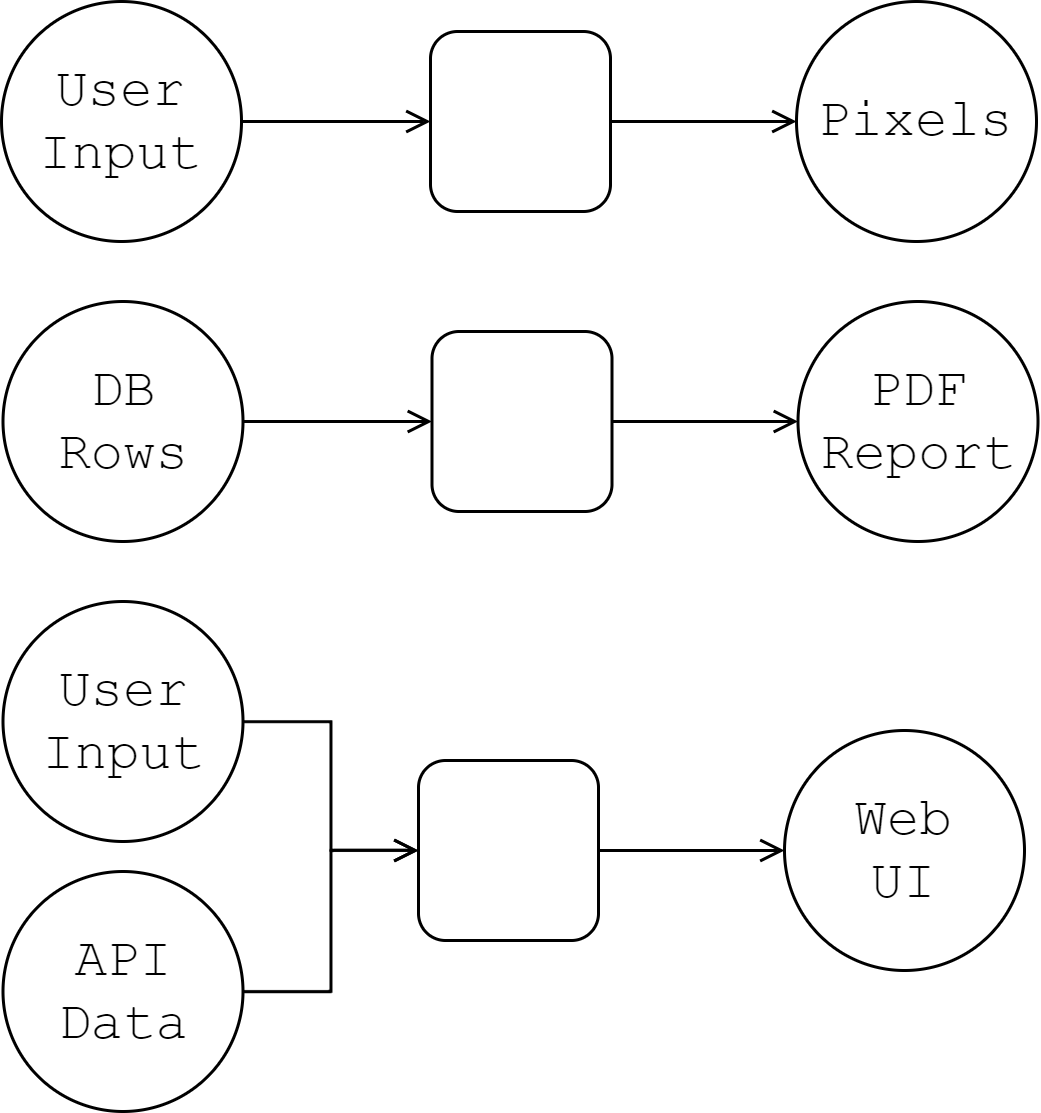
\includegraphics{lesson12/programs-transform-data.png}
\end{figure}

In each of these cases, a program transforms one or more pieces of data
into some other piece of data. Functions are the building blocks that
describe these data transformations. Functions can be composed out of
other functions to build more useful, higher-level transformations.

We can think about functional programming as a description of data in
motion. Unlike imperative code that makes us think about algorithms in
terms of statements that assign and mutate data, we can think of our
code as a description of how data flows through our program. Functions
are the key to writing such declarative programs. Each function has zero
or more input values (argument), and they always return some output
value\footnote{In practice, many functions return \texttt{nil}, which is
  a value that denotes the absence of any meaningful value. Functions
  that return \texttt{nil} are often called for side effects.}.\index{side effects!within functions}

\begin{figure}[H]
\caption{Functions map input to output}
\centering
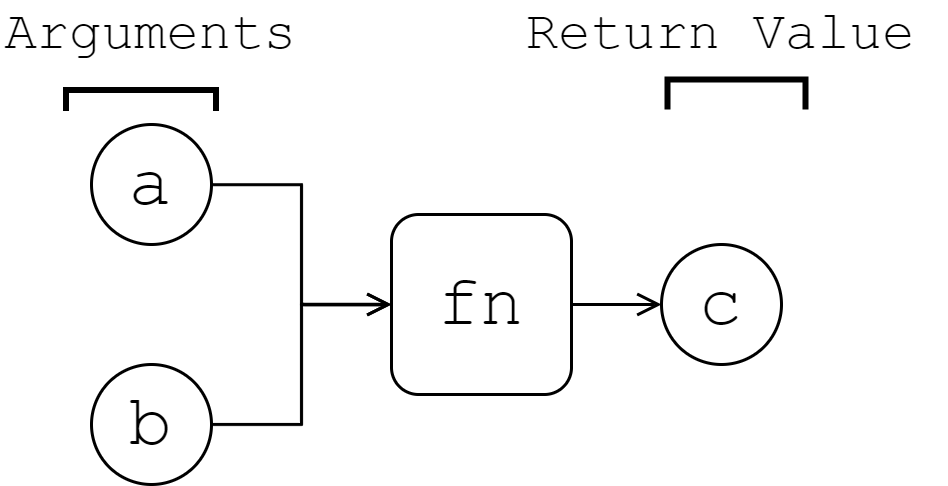
\includegraphics{lesson12/function-transformation.png}
\end{figure}

\section{Defining and Calling Functions}

\index{data types!functions}Just like strings, numbers, and keywords, ClojureScript functions are
values. This means that they can be assigned to vars, passed into other
functions as arguments, and returned from other functions. This should
not be a new concept for JavaScript programmers, since JavaScript
functions are also first-class values:

\begin{lstlisting}[language=JavaScript, caption={First-class functions in JavaScript}]
const removeBy = (pred) => {                               %\circled{1}%
    return list =>                                         %\circled{2}%
        list.reduce((acc, elem) => {
            if (pred(elem)) {
                return acc;
            }
            return acc.concat([elem]);
        }, []);
}

const removeReds = removeBy(                               %\circled{3}%
    product => product.color === 'Red'
);

removeReds([
    { sku: '99734N', color: 'Blue' },
    { sku: '99294N', color: 'Red' },
    { sku: '11420Z', color: 'Green' },
]);
\end{lstlisting}

\begin{enumerate}[label=\protect\circled{\arabic*}]
\tightlist
\item
  Assign a function to a variable, \texttt{removeBy}
\item
  Return a function
\item
  Pass a function as an argument to another function
\end{enumerate}

A direct translation\footnote{This code sample is intended to be a
  direct translation in order to illustrate the similarity between
  functions in ClojureScript and JavaScript. It is not idiomatic
  ClojureScript, and it does not take advantage of the standard library.}
of this code to ClojureScript is pleasantly straightforward:

\begin{lstlisting}[language=Clojure, caption={First-class functions in ClojureScript}]
(def remove-by                                             %\circled{1}%
  (fn [pred]
    (fn [list]                                             %\circled{2}%
      (reduce (fn [acc elem]
                (if (pred elem) acc (conj acc elem)))
              []
              list))))

(def remove-reds                                           %\circled{3}%
  (remove-by (fn [product] (= "Red" (:color product)))))

(remove-reds
  [{:sku "99734N" :color "Blue"}
   {:sku "99294N" :color "Red"}
   {:sku "11420Z" :color "Green"}])
\end{lstlisting}

\begin{enumerate}[label=\protect\circled{\arabic*}]
\tightlist
\item
  Assign a function to a variable, \texttt{remove-by}
\item
  Return a function
\item
  Pass a function as an argument to another function
\end{enumerate}

Since JavaScript was designed with a lot of the features of Scheme\index{Scheme} -
another Lisp - in mind, it should come as no surprise that functions
work similarly across both languages. The primary differences are
syntactical rather than semantic. So with that, let's take a look at the
syntax for defining functions.


\subsection{fn and defn}

\index{functions!definition}Functions may be defined with the \texttt{fn} special form. In its most
basic version \texttt{fn} takes a vector of parameters and one or more
expressions to evaluate. When the function is called, the arguments that
it is called with will be bound to the names of the parameters, and the
body of the function will be evaluated. The function will evaluate to
the the value of the last expression in its body. As an example, let's
take a function that checks whether one sequence contains every element
in a second sequence:

\begin{lstlisting}[language=Clojure, caption={Function expression}]
(fn [xs test-elems]                                        %\circled{1}%
  (println "Checking whether" xs                           %\circled{2}%
           "contains each of" test-elems)
  (let [xs-set (into #{} xs)]                              %\circled{3}%
    (every? xs-set test-elems)))
\end{lstlisting}

\begin{enumerate}[label=\protect\circled{\arabic*}]
\tightlist
\item
  Declare a function that takes 2 parameters
\item
  The first expression is evaluated for side effects, and its result is
  discarded
\item
  The entire function takes on the value of the last expression
\end{enumerate}

This example illustrates the basic form of \texttt{fn} where there is a
parameter vector and a body consisting of 2 expressions. Note that the
first expression logs some debug information and does not evaluate to
any meaningful value. The function itself takes on the value of the
final expression where \texttt{xs} and \texttt{test-elems} are
substituted with the actual values with which the function is called:

\begin{lstlisting}[language=Clojure]
(let [xs-set (into #{} xs)]
  (every? xs-set test-elems))
\end{lstlisting}

\subsubsection{Anonymous Function Shorthand}

\index{functions!anonymous shorthand}There is another even terser syntax for anonymous functions that saves a
few keystrokes by omitting the \texttt{fn} and the named argument list.
In the next example, we use this abbreviated syntax.

\begin{lstlisting}[language=Clojure, caption={Shorter anonymous functions}]
#(let [xs-set (into #{} %\%%1)]
   (every? xs-set %2)))
\end{lstlisting}

As we can see, the function itself is defined with \texttt{\#(...)}, and
each argument is referred to by its position - \texttt{\%1},
\texttt{\%2}, etc. If the function takes only 1 argument, then the
argument may be referred to simply as \texttt{\%}:

\begin{lstlisting}[language=Clojure]
(#(str "Hello " %\%%) "world")
;; => "Hello world"
\end{lstlisting}

While this syntax is handy, we should only use it for extremely small
functions whose intent is readily apparent. In the normal case, we
should prefer to use the slightly longer syntax for the clarity that
comes with named arguments. Also, for a function that takes more than
one argument, this syntax usually introduces more confusion than
necessary. It is still fairly common in ClojureScript code and is often
used for event callbacks.


\subsubsection{Defining Named Functions}

You may have noticed that while we have declared a useful function, we
do not have any way to call it because it lacks a name. This is where
\texttt{defn} comes in - it is a shorthand for declaring a function and
binding it to a var at the same time:

\begin{lstlisting}[language=Clojure, caption={Defining functions}]
(def contains-every?                                       %\circled{1}%
  (fn [xs test-elems]
    ;; function body...
    ))

(defn contains-every? [xs test-elems]                      %\circled{2}%
  ;; function body...
)
\end{lstlisting}

\begin{enumerate}[label=\protect\circled{\arabic*}]
\tightlist
\item
  Bind the anonymous function to a var, \texttt{contains-every?}
\item
  Define the function and bind it at the same time with \texttt{defn}
\end{enumerate}

As we can see, \texttt{defn} is a useful shorthand when we want to
create a named function.

In order to keep our programs clean, we usually group related functions
together into a \emph{namespace}.\index{namespaces} When we bind\index{binding} a function to a var using
either \texttt{def} or \texttt{defn}, the function becomes public and
can be required from any other namespace. In ClojureScript, vars\index{vars} are
exported by default unless explicitly made private\footnote{Functions
  can be made private by declaring them with \texttt{defn-} instead of
  \texttt{defn}.}. Unlike object-oriented programming, which seeks to
hide all but the highest-level implementation, Clojure is about
visibility and composing small functions - often from different
namespaces. We will look at namespaces and visibility in much greater
detail in Lesson 23.

\subsection{Variations of defn}

The basic form of \texttt{defn} that we just learned is by far the most
common, but there are a couple of extra pieces of syntax that may be
used.

\subsubsection{Multiple Arities}

\index{functions!arities}First, a function can be declared with multiple \emph{arities} - that
is, its behavior can vary depending on the number or arguments given. To
declare multiple arities, each parameter list and function body is
enclosed in a separate list following the function name.

\begin{lstlisting}[language=Clojure, caption={Function arities}]
(defn my-multi-arity-fn
 ([a] (println "Called with 1 argument" a))                %\circled{1}%
 (                                                         %\circled{2}%
  [a b]                                                    %\circled{3}%
  (println "Called with 2 arguments" a b)                  %\circled{4}%
 )
 ([a b c] (println "Called with 3 arguments" a b c)))

(defn my-single-arity-fn [a]                               %\circled{5}%
  (println "I can only be called with 1 argument"))
\end{lstlisting}

\begin{enumerate}[label=\protect\circled{\arabic*}]
\tightlist
\item
  Unlike the basic \texttt{defn} form, each function implementation is
  enclosed in a list
\item
  For each function implementation, the first element in the list is the
  parameter vector
\item
  \ldots{}followed by one or more expressions, forming the body of the
  implementation for that arity
\item
  Remember that for a single-arity function, the parameters and
  expressions that form the body of the function need not be enclosed in
  a list
\end{enumerate}

Multiple arity functions are often used to supply default parameters.
Consider the following function that can add an item to a shopping cart.
The 3-ary version lets a quantity be specified along with the
\texttt{product-id}, and the 2-ary version calls this 3-ary version with
a default quantity of \texttt{1}:

\begin{lstlisting}[language=Clojure]
(defn add-to-cart
 ([cart id] (add-to-cart cart id 1))
 ([cart id quantity]
  (conj cart {:product (lookup-product id)
              :quantity quantity})))
\end{lstlisting}

This is one area that is surprisingly different than JavaScript because
functions in ClojureScript can only be called with an arity that is
declared explicitly. That is, a function that is declared with a single
parameter may only be called with a single argument, a function that is
declared with two parameters may only be called with 2 arguments, and so
forth.

\subsubsection{Docstrings}

\index{functions!docstrings}A function can also contain a docstring - a short description of the
function that serves as inline documentation. When using a docstring, it
should come immediately after the function name:

\begin{lstlisting}[language=Clojure, caption={Documenting a function}]
(defn make-inventory
  "Creates a new inventory that initially contains no items.
  Example:
  (assert
    (== 0 (count (:items (make-inventory)))))"
  []
  {:items []})
\end{lstlisting}

The advantage of using a docstring rather than simply putting a comment
above the function is that the docstring is metadata that is preserved
in the compiled code and can be accessed programmatically using the
\texttt{doc} function that is built into the REPL:

\begin{verbatim}
dev:cljs.user=> (doc make-inventory)
-------------------------
cljs.user/make-inventory
([])
  Creates a new inventory that initially contains no items.
  Example:
  (assert
    (== 0 (count (:items (make-inventory)))))
nil
\end{verbatim}


\subsubsection{Pre- and post-conditions}

\index{design by contract}ClojureScript draws some inspiration from the \emph{design by contract}
concept pioneered by the Eiffel\index{Eiffel}
programming language. When we define a function, we can specify a
contract about what that function does in terms of pre-conditions and
post-conditions. These are checks that are evaluated immediately before
and after the function respectively. If one of these checks fails, a
JavaScript \texttt{Error} is thrown.

A vector of pre- and post-conditions may be specified in a map
immediately following the parameter list, using the \texttt{:pre} key
for pre-conditions and the \texttt{:post} key for post-conditions. Each
condition is specified as an expression within the \texttt{:pre} or
\texttt{:post} vector. They may both refer to the arguments of the
function by parameter name, and post-conditions may also reference the
return value of the function using \texttt{\%}.

\begin{lstlisting}[language=Clojure, caption={Preconditions and postconditions}]
(defn fractional-rate [num denom]
  {:pre [(not= 0 denom)]                                    %\circled{1}%
   :post [(pos? %\%%) (<= %\%% 1)]}                               %\circled{2}%
  (/ num denom))

(fractional-rate 1 4)
;; 0.25

(fractional-rate 3 0)
;; Throws:
;; #object[Error Error: Assert failed: (not= 0 denom)]
\end{lstlisting}

\begin{enumerate}[label=\protect\circled{\arabic*}]
\tightlist
\item
  A single pre-condition is specified, ensuring that the \texttt{denom}
  is never zero
\item
  Two post-conditions are specified, ensuring that the result is a
  positive number that is less than or equal to \texttt{1}.
\end{enumerate}


\subsection{You Try It}

\begin{itemize}
\tightlist
\item
  In the REPL, define a function that takes 1 argument, then call it
  with 2 arguments. What happens?
\item
  Try enclosing the parameter list and function body of a single-arity
  function in a list. Is this valid?
\item
  Combine all 3 of the advanced features of \texttt{defn} that we have
  learned to create a function with a docstring, multiple arities, and
  pre-/post-conditions.
\end{itemize}


\section{Functions as Expressions}

\index{evaluation!of function calls}Now that we have learned how to define functions mechanically, let's
take a step back and think about what a function is. Think back to
Lesson 4:
Expressions and Evaluation where we developed a mental model of
evaluation in ClojureScript. Recall how an interior s-expression is
evaluated and its results substituted into its outer expression:

\begin{verbatim}
(* (+ 5 3) 2)
;; => (* 8 2)
;; => 16
\end{verbatim}

In Lesson 4, we took it for granted that an s-expression like
\texttt{(+\ 5\ 3)} evaluates to \texttt{8}, but we did not consider how
this happened. We need to expand that mental model of evaluation to
account for what happens a function is called.

\index{functions!parameters}When we define a function, we declare a list of parameters. These are
called the \texttt{formal\ parameters} of the function. The function
body is free to refer to any of these formal parameters. When the
function is called, the call is replaces with the body of the function
where every instance of the formal parameters is replaced with the
argument that was passed in - called the \texttt{actual\ parameters}.
While this is a bit confusing to explain, a quick example should help
clarify:

\begin{lstlisting}[language=Clojure]
(defn hypotenuse [a b]                                     %\circled{1}%
  (Math/sqrt
    (+ (* a a)
       (* b b))))

(str "the hypotenuse is: " (hypotenuse 3 4))               %\circled{2}%

(str "the hypotenuse is: " (Math/sqrt                      %\circled{3}%
                             (+ (* 3 3)
                                (* 4 4))))

(str "the hypotenuse is: " 5)                              %\circled{4}%

"the hypotenuse is: 5"                                     %\circled{5}%
\end{lstlisting}

\begin{enumerate}[label=\protect\circled{\arabic*}]
\tightlist
\item
  Define a function called \texttt{hypotenuse}
\item
  Call the function we just defined
\item
  Replace the call to the function with the body from the function
  definition, substituting \texttt{3} in the place of \texttt{a} and
  \texttt{4} in the place of \texttt{b}
\item
  Evaluate the resulting expression
\item
  Continue evaluation until we have produced a final value
\end{enumerate}

\begin{figure}[H]
\caption{Parameter substitution}
\centering
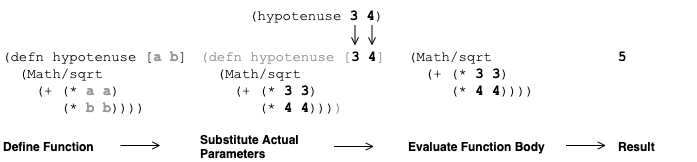
\includegraphics[width=12cm]{lesson12/parameter-substitution.png}
\end{figure}

When we think about a function as a template for another expression, it
fits nicely into our existing model of evaluation. Functions in
ClojureScript are a simpler concept than in JavaScript because they do
not have an implicit mutable context. In JavaScript, standard functions
have a special \index{JavaScript!this@\texttt{this}}\texttt{this} variable that can refer to some object that
the function can read and mutate. Depending on how the function was
defined, \texttt{this} may refer to different things, and even
experienced developers sometimes get tripped up by \texttt{this}.
ClojureScript functions - by contrast - are \emph{pure} and do not carry
around any additional state. It is this purity that makes them fit well
into our model of expression evaluation.


\subsection{Closures}

\index{closure}Although ClojureScript functions do not have automatic access to some
shared mutable state by default, there is one more detail that we have
to account for when reasoning about how a function is evaluated. In
ClojureScript, just like in JavaScript, functions have lexical scope,
which means that they can reference any symbol that is visible at the
site where the function is defined. When a function references a
variable from its \index{lexical scope}lexical scope, we say that it creates a
\emph{closure}. For example, we can reference any vars previously
declared in the same namespace:

\begin{lstlisting}[language=Clojure, caption={Lexical closures}]
(def http-codes                                            %\circled{1}%
  {:ok 200
   :created 201
   :moved-permanently 301
   :found 302
   :bad-request 400
   :not-found 404
   :internal-server-error 500})

(defn make-response [status body]
  {:code (get http-codes status)                           %\circled{2}%
   :body body})
\end{lstlisting}

\begin{enumerate}[label=\protect\circled{\arabic*}]
\tightlist
\item
  Define a var in the current namespace
\item
  Referencing this var inside our function creates a closure over it
\end{enumerate}

Since ClojureScript has the concept of higher-order functions, a
function that is returned from another function can also reference
variables from the parent function's scope:

\begin{lstlisting}[language=Clojure, caption={Capturing values}]
(def greeting "Hi")                                        %\circled{1}%

(defn make-greeter [greeting]                              %\circled{2}%
  (fn [name]
    (str greeting ", " name)))                             %\circled{3}%

((make-greeter "Здрасти") "Anton")
;; => "Здрасти, Anton"
\end{lstlisting}

\begin{enumerate}[label=\protect\circled{\arabic*}]
\tightlist
\item
  The symbol \texttt{greeting} will refer to a var with the value of
  \texttt{Hi} within this namespace
\item
  Within this function, \texttt{greeting} will refer to whatever
  argument is passed in, not the namespace-level var
\item
  The inner function closes over the \texttt{greeting} from it's parent
  function's scope
\end{enumerate}

In this example, the function returned from \texttt{make-greeter}
creates a closure over \texttt{greeting}. If we were to call
\texttt{(make-greeter\ "Howdy")}, the resulting function would always
substitute \texttt{"Howdy"} for \texttt{greeter} whenever it was
evaluated. Even though there was another value bound to the symbol
\texttt{greeting} outside the \texttt{make-greeter} function, the inner
function is not able to see it because there is another symbol with the
same name \emph{closer} to the function itself. We say that the
namespace-level \texttt{greeting} is \emph{shadowed}\index{lexical scope!shadowing} by the inner
\texttt{greeting}. We will study closures in more detail in
Lesson 21
and see how we need to modify our mental model of evaluation in order to
accommodate them.

\subsection{Functions as Abstraction}

As we saw above, functions are ways to re-use expressions, but they are
much more than that. They are the ClojureScript developer's primary
means of abstraction. Functions hide the details of some transformation
behind a name. Once we have abstracted an expression, we don't need to
be concerned anymore with how it is implemented. As long as it meets our
expectations, it should not matter to us anymore what happens under the
hood. As a trivial example, lets look at several potential
implementations for an \texttt{add} function.

\begin{lstlisting}[language=Clojure, caption={Two versions of \texttt{add}}]
(defn add [x y]                                            %\circled{1}%
  (+ x y))

(defn add [x y]                                            %\circled{2}%
  (if (<= y 0)
    x
    (add (inc x) (dec y))))

(defn add [x y]                                            %\circled{3}%
  47)

(add 17 23)                                                %\circled{4}%
\end{lstlisting}

\begin{enumerate}[label=\protect\circled{\arabic*}]
\tightlist
\item
  A basic function to add two numbers
\item
  Another function for adding. It's less efficient, but it works.
\item
  A very opinionated function for adding. Unfortunately, it is almost
  always wrong.
\item
  Call the \texttt{add} function. All we know is that it is supposed to
  add our numbers.
\end{enumerate}

The real power comes when we move from specific, granular function to
higher levels of abstraction. In ClojureScript, we often find ourselves
starting a new project by creating many small functions that describe
small details and processes in the problem domain then using these
functions to define slightly less granular details and processes. This
practice of ``bottom-up'' programming\index{bottom-up programming} gives us the ability to focus on
only the level of abstraction that we are interested in without caring
about either the lower-level functions that it is composed of or the
higher-level functions in which it serves as an implementation detail.


\subsection{Quick Review}

\begin{itemize}
\tightlist
\item
  Define a function using \texttt{my-inc} that returns the increment of
  a number. How would you define a function with the same name without
  using \texttt{defn}?
\item
  What is the difference between the \emph{formal parameters} and
  \emph{actual parameters}
\item
  What does \emph{shadowing} mean in the context of a closure?
\end{itemize}


\section{Recursion 101}

\index{looping constructs!recursion} As the last topic of this lesson, we will cover recursive functions. As
we mentioned earlier, a recursive function is simply a function that can
call itself. We made use of \texttt{loop/recur} in the last chapter to
implement recursion within a function. Now let's see how to implement a
recursive function using the classic factorial function.

\begin{lstlisting}[language=Clojure, caption={Recursive factorial}]
(defn factorial [n]
  (if (<= n 1)
    n                                                      %\circled{1}%
    (* n (factorial (dec n)))))                            %\circled{2}%
\end{lstlisting}

\begin{enumerate}[label=\protect\circled{\arabic*}]
\tightlist
\item
  Base case - do not call \texttt{factorial} again
\item
  Recursive case, call \texttt{factorial} again
\end{enumerate}

This example should be unsurprising to readers with prior JavaScript
experience. Recursion works essentially the same in ClojureScript as it
does in JavaScript: each recursive call grows the stack, so we need to
take care not to overflow the stack.\index{call stack} However, if our function is tail
recursive - that is, if it calls itself as the very last step in its
evaluation - then we can use the \texttt{recur} special form just as we
did with \texttt{loop} in the last lesson. The only difference is that
if it is not within a \texttt{loop}, \texttt{recur} will recursively
call its containing function. Knowing this, we can write a
tail-recursive version of \texttt{factorial} that will not grow the
stack:

\begin{lstlisting}[language=Clojure, caption={Tail-recursive factorial}]
(defn factorial
 ([n] (factorial n 1))
 ([n result]
  (if (<= n 1)
    result
    (recur (dec n) (* result n)))))
\end{lstlisting}

ClojureScript is able to optimize this recursive function into a simple
loop, just as it did with \texttt{loop/recur} in the last lesson.


\subsection{Quick Review}

\begin{itemize}
\tightlist
\item
  If you are uncertain how recursion works, go back and read from
  ``Recursion 101''.
\end{itemize}


\section{Summary}

In this lesson, we took a fairly detailed look at functions in
ClojureScript. We learned the difference between \texttt{fn} and
\texttt{defn}, and we studied the various forms that \texttt{defn} can
take. We considered the model of evaluation for functions and presented
them as a means of extracting common expressions. Finally, we looked at
recursive functions and saw how to use \texttt{recur} to optimize
tail-recursive functions. While JavaScript and ClojureScript look at
functions in a similar way, we made sure to point out the areas of
difference so as to avoid confusion moving forward.

\chapter{Interacting With JavaScript Data}

One of the advantages of ClojureScript is its excellent interoperability
with JavaScript. When Clojure was first introduced, one of its primary
goals was providing simple integration with existing Java code.
ClojureScript continues in this spirit of valuing integration with its
host platform. We will deal with JavaScript interoperability to a
greater extent later, but at this point, we will concern ourselves with
creating and manipulating JavaScript data structures.

\begin{center}\rule{0.5\linewidth}{0.5pt}\end{center}

\textbf{In this lesson:}

\begin{itemize}
\tightlist
\item
  Convert between ClojureScript and JavaScript data types
\item
  Integrate ClojureScript code with an existing JavaScript codebase
\item
  Understand the implications of using mutable JavaScript objects and
  arrays
\end{itemize}

\begin{center}\rule{0.5\linewidth}{0.5pt}\end{center}


\section{Example: Integration With Legacy Code}

Imagine that we have decided to slowly migrate a legacy JavaScript
application to ClojureScript (an excellent choice). However, due to the
size of the codebase, it is more practical to migrate one piece at a
time. In the meantime, we need to interact with our legacy application,
a classroom management application, from ClojureScript. We will need to
read a list of scores from the legacy application, perform modifications
in ClojureScript, and send the results back to the JavaScript
application. Fortunately for us, ClojureScript has excellent
interoperability with JavaScript, so let's learn how it's done!


\section{Using Conversion Functions}

\index{data types!converting to/from JavaScript}When we are working with an existing JavaScript codebase or libraries,
chances are that we will be passing JavaScript data structures around,
but we would like to treat them as ClojureScript data within our
application. ClojureScript provides two handy functions for converting
between JavaScript and ClojureScript data structures:
\texttt{js-\textgreater{}clj} for converting from JavaScript and
\texttt{clj-\textgreater{}js} for converting to JavaScript. We can
easily use these functions to convert data to ClojureScript structures
coming into our program and back to JavaScript on the way out.

Let's try this out by opening up the REPL and the browser tab that it is
connected to. Open the dev tools and create an object called
\texttt{testScores} that looks something like the following:

\begin{lstlisting}[language=JavaScript, caption={Creating a JS object}]
var testScores = [                                         %\circled{1}%
  { id: 1, score: 86, gradeLetter: "B" },                  %\circled{2}%
  { id: 2, score: 93, gradeLetter: "A" },
  { id: 3, score: 78, gradeLetter: "C" },
];
\end{lstlisting}

\begin{enumerate}[label=\protect\circled{\arabic*}]
\tightlist
\item
  The top-level structure is an array of objects
\item
  The nested objects have \texttt{id}, \texttt{score}, and
  \texttt{gradeLetter} properties
\end{enumerate}

This creates a global JavaScript variable called \texttt{testScores},
which we can access from the REPL. ClojureScript creates a namespace
(think a module for collecting functions and data) called \texttt{js}
that contains all of the global variables that are available within the
browser. For example, we can access the \texttt{document} object with
\texttt{js/document}, the \texttt{window} object with
\texttt{js/window}, etc.

\begin{figure}[h]
\caption{Sharing data between browser and REPL}
\centering
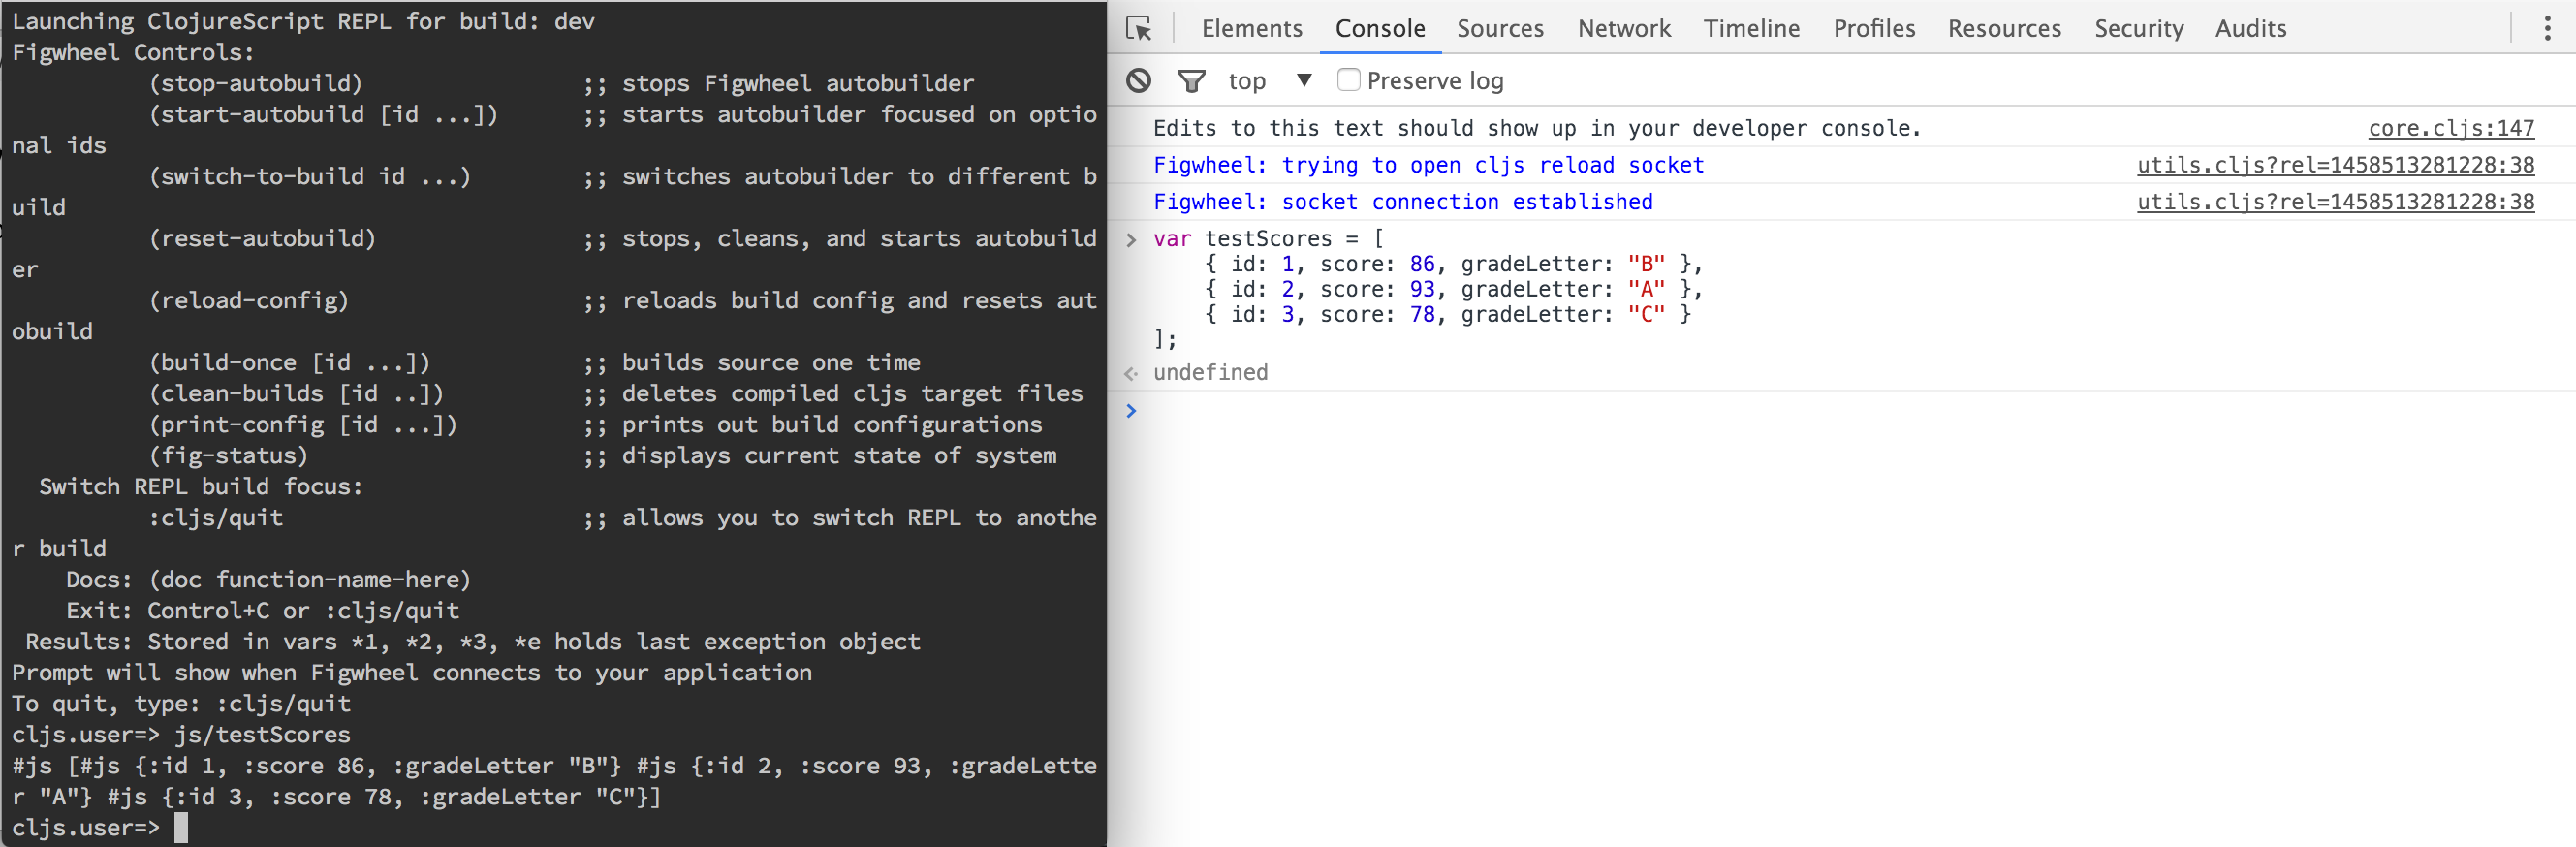
\includegraphics{lesson13/sharing-data.png}
\end{figure}

We can use the REPL to inspect this variable, convert it to a
ClojureScript data structure, modify it and write a new version back out
the the \texttt{testScores} variable.

\begin{lstlisting}[language=Clojure, caption={Converting between JavaScript and ClojureScript data}]
cljs.user=> (def cljs-scores (js->clj js/testScores))      %\circled{1}%
#'cljs.user/cljs-scores

cljs.user=> cljs-scores
[{"id" 1, "score" 86, "gradeLetter" "B"}
{"id" 2, "score" 93, "gradeLetter" "A"}
{"id" 3, "score" 78, "gradeLetter" "C"}]

cljs.user=> (conj cljs-scores                              %\circled{2}%
                  {"id" 4, "score" 87, "gradeLetter" "B"})
[{"id" 1, "score" 86, "gradeLetter" "B"}
{"id" 2, "score" 93, "gradeLetter" "A"}
{"id" 3, "score" 78, "gradeLetter" "C"}
{"id" 4, "score" 87, "gradeLetter" "B"}]

cljs.user=> cljs-scores
[{"id" 1, "score" 86, "gradeLetter" "B"}
{"id" 2, "score" 93, "gradeLetter" "A"}
{"id" 3, "score" 78, "gradeLetter" "C"}]

cljs.user=> (def updated-scores                            %\circled{3}%
              (conj cljs-scores {"id" 4, "score" 87, "gradeLetter" "B"}))
#'cljs.user/updated-scores

cljs.user=> (set! js/testScores (clj->js updated-scores))  %\circled{4}%
#js [#js {:id 1, :score 86, :gradeLetter "B"}
#js {:id 2, :score 93, :gradeLetter "A"}
#js {:id 3, :score 78, :gradeLetter "C"}
#js {:id 4, :score 87, :gradeLetter "B"}]
\end{lstlisting}

\begin{enumerate}[label=\protect\circled{\arabic*}]
\tightlist
\item
  Convert \texttt{testScores} to a ClojureScript value
\item
  Create a modified value by appending a new score and verify that the
  value in the var \texttt{cljs-scores} was not changed
\item
  Bind the updated scores to the \texttt{updated-scores} var
\item
  Convert the updated scores back to a JavaScript object and update
  \texttt{testScores} to the new value
\end{enumerate}

We can inspect the \texttt{testScores} variable in the browser to make
sure that it has been changed to include the new score.

\begin{figure}[h]
\caption{Checking the updated scores}
\centering
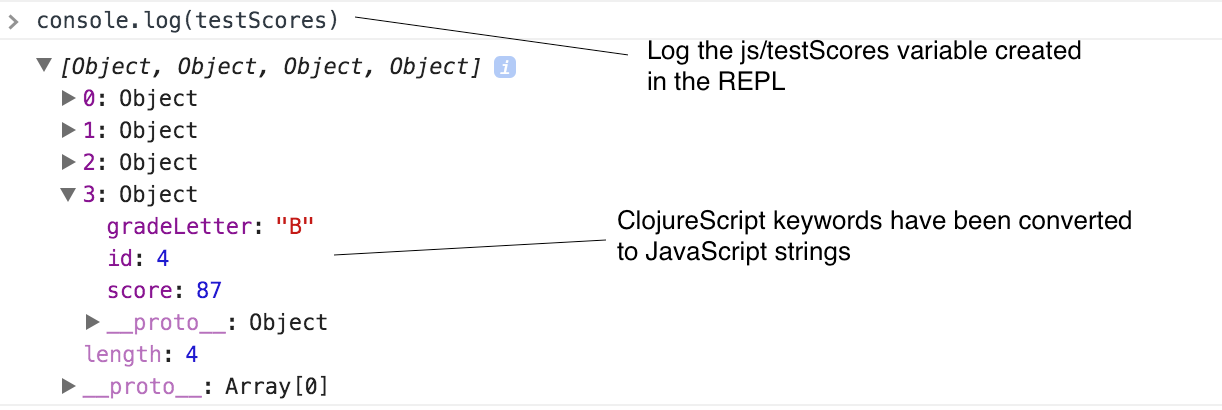
\includegraphics[width=4.07in]{lesson13/checking-scores.png}
\end{figure}

\subsection{Quick Review}

We still have a reference to the \texttt{js/testScores} variable.

\begin{itemize}
\tightlist
\item
  What will happen if we change this variable in the browser's developer
  tools and print it out from ClojureScript?
\item
  Will changing this JavaScript variable affect our \texttt{cljs-scores}
  variable?
\end{itemize}

\begin{notice}[title={Lossy Conversions}]
Since ClojureScript has richer data types than JavaScript,
\texttt{clj-\textgreater{}js} is a \emph{lossy} operation. For instance, sets are
converted to JS arrays, and keywords and symbols are converted to
strings. This means that some ClojureScript value contained in the var,
\texttt{x}, is not always equal to \texttt{(js-\textgreater{}clj (clj-\textgreater{}js x))}.
For instance, if we have a set, \texttt{\#\{``Lucy'' ``Ricky'' ``Fred'' ``Ethel''\}},
and we convert this to JavaScript, we will end up with an
array: \texttt{{[}``Ricky'', ``Fred'', ``Lucy'', ``Ethel''{]}} (remember, sets
are not ordered, so the order in which the elements appear when
converted to an array is arbitrary). If we convert this array back to
ClojureScript, we end up with the vector, \texttt{{[}``Ricky'' ``Fred'' ``Lucy''
``Ethel''{]}}, not the set that we started with, as we demonstrate below.

\begin{verbatim}
cljs.user=> (def characters #{"Lucy" "Ricky" "Fred" "Ethel"})
#'cljs.user/characters
cljs.user=> (def js-characters (clj->js characters))
#'cljs.user/js-characters
cljs.user=> js-characters
#js ["Ricky" "Fred" "Lucy" "Ethel"]
cljs.user=> (js->clj js-characters)
["Ricky" "Fred" "Lucy" "Ethel"]
cljs.user=> (= characters (js->clj js-characters))
false
\end{verbatim}
\end{notice}

\subsection{You Try It}

\begin{itemize}
\tightlist
\item
  Create a JavaScript object from the REPL and make it available as
  \texttt{window.myVar}.
\item
  Create a JavaScript object in the dev tools called \texttt{jsObj} and
  modify it using the \texttt{set!} function in the ClojureScript REPL
\end{itemize}


\section{Working with JavaScript Data Directly}

Although it is very common to convert JavaScript data from the ``outside
world'' to ClojureScript data before working with it, it is also
possible to create and modify JavaScript data directly from within
ClojureScript. ClojureScript numbers, strings, and booleans are the same
as their JavaScript counterparts, so they can be handled natively from
ClojureScript.

\subsection{Using Objects}

Objects can be created either with the \texttt{js-obj} function or the
literal syntax, \texttt{\#js\ \{\}}.

\begin{lstlisting}[language=Clojure, caption={Constructing JavaScript objects}]
cljs.user=> (js-obj "isJavaScript" true, "type" "object")  %\circled{1}%
#js {:isJavaScript true, :type "object"}

cljs.user=> #js {"isJavaScript" true, "type" "object"}     %\circled{2}%
#js {:isJavaScript true, :type "object"}
\end{lstlisting}

\begin{enumerate}[label=\protect\circled{\arabic*}]
\tightlist
\item
  Creating an object with the \texttt{js-obj} function
\item
  Creating an object with the literal \texttt{\#js\ \{\}} syntax
\end{enumerate}

The \texttt{js-obj} function takes an even number of arguments, which
are expected to be pairs of key, value. The literal syntax looks like a
ClojureScript map proceeded by \texttt{\#js}. Both of these forms
produce identical JavaScript objects, but the literal syntax is by far
the most common.

\index{property access}We can get properties on JavaScript objects with the property access
syntax: \texttt{(.-property\ object)}, and we can use the \texttt{set!}
function to update a property.

\begin{lstlisting}[language=Clojure]
cljs.user=> (def js-hobbit #js {"name" "Bilbo Baggins", "age" 111})
#'cljs.user/js-hobbit
cljs.user=> (.-age js-hobbit)
111
\end{lstlisting}

A variant of the property access syntax supports accessing properties
inside nested objects, similar to chaining property lookups on
JavaScript objects. For instance, in JavaScript, we could do the
following (if we were confident that all of the intermediate properties
were valid):

\begin{lstlisting}[language=JavaScript, caption={Nested lookup in JavaScript}]
var settings = {                                           %\circled{1}%
  personal: {
    address: {
      street: "123 Rolling Hills Dr",
    },
  },
};

// Prints "123 Rolling Hills Dr"
console.log(settings.personal.address.street);             %\circled{2}%
\end{lstlisting}

\begin{enumerate}[label=\protect\circled{\arabic*}]
\tightlist
\item
  A nested JavaScript object
\item
  Accessing a nested property
\end{enumerate}

Using property access in ClojureScript accomplishes the same task. The
syntax is slightly different from a normal property access:
\texttt{(..\ obj\ -propOne\ -propTwo)}.

\begin{lstlisting}[language=Clojure, caption={Nested lookup in ClojureScript}]
(println
  (.. settings -personal -address -street))
; Prints "123 Rolling Hills Dr"
\end{lstlisting}

In addition to letting us read properties on a potentially nested
object, ClojureScript provides the \texttt{set!} function to mutate
objects. This function takes a property access along with a new value to
set, and it mutates the object at the specified property, returning the
value that was supplied.

\begin{lstlisting}[language=Clojure]
cljs.user=> (set! (.-name js-hobbit) "Frodo")              %\circled{1}%
"Frodo"

cljs.user=> (set! (.-age js-hobbit) 33)
33

cljs.user=> js-hobbit                                      %\circled{2}%
#js {:name "Frodo", :age 33}
\end{lstlisting}

\begin{enumerate}[label=\protect\circled{\arabic*}]
\tightlist
\item
  Setting two properties on the \texttt{js-hobbit} object
\item
  \texttt{set!} mutates the object
\end{enumerate}


\subsubsection{Experiment}

Since property access supports nested properties, it only makes sense
that the the \texttt{set!} function would support setting nested
properties. Use the REPL to try to find the correct syntax for setting
the following student's grade in her Physics class:

\begin{lstlisting}[language=Clojure]
(def student #js {"locker" 212
                  "grades" {"Math" "A",
                            "Physics" "B",
                            "English" "A+"}})
\end{lstlisting}

Unlike the functions that we have seen that operate on ClojureScript
data, \texttt{set!} actually modifies the object in-place. This is
because we are working with mutable JavaScript data.

\subsection{Using Arrays}

Just like there is a function and a literal syntax for creating
JavaScript objects, we can use the \texttt{array} function or the
\texttt{\#js\ {[}{]}} literal for creating JavaScript arrays.

\begin{lstlisting}[language=Clojure, caption={Creating JavaScript arrays}]
cljs.user=> (array "foo" "bar" "baz")
#js ["foo" "bar" "baz"]

cljs.user=> #js [1 3 5 7 11]
#js [1 3 5 7 11]
\end{lstlisting}

\index{array access}For array access, we can use the \texttt{aget} and \texttt{aset}
functions. \texttt{aget} takes a JavaScript array and an index into that
array and returns the element at that index. \texttt{aset} has an
additional parameter, which is the value to set at the specified index.
Like \texttt{set!}, \texttt{aset} mutates the array in place.

\begin{lstlisting}[language=Clojure, caption={Getting and setting array elements}]
cljs.user=> (def primes #js [1 3 5 7 11])                  %\circled{1}%
#'cljs.user/primes

cljs.user=> (aget primes 2)                                %\circled{2}%
5

cljs.user=> (aset primes 5 13)                             %\circled{3}%
13

cljs.user=> primes                                         %\circled{4}%
#js [1 3 5 7 11 13]
\end{lstlisting}

\begin{enumerate}[label=\protect\circled{\arabic*}]
\tightlist
\item
  Bind a var to a JavaScript array
\item
  Get the element at index \texttt{2}
\item
  Get the element at index \texttt{5} to \texttt{13}
\item
  \texttt{aset} has mutated the array
\end{enumerate}

We can also access the JavaScript array methods by using,
\texttt{(.functionName\ array\ args*)}. This is the standard syntax for
calling a method on a JavaScript object, which we will explain in much
more detail later.

\begin{lstlisting}[language=Clojure, caption={Using JavaScript array methods}]
cljs.user=> (.indexOf primes 11)                           ;; <1>
4

cljs.user=> (.pop primes)                                  ;; <2>
13

cljs.user=> primes
#js [1 3 5 7 11]
\end{lstlisting}

\begin{enumerate}[label=\protect\circled{\arabic*}]
\tightlist
\item
  Call the \texttt{indexOf} method on \texttt{primes} - equivalent to
  \texttt{primes.indexOf(11)} in JavaScript
\item
  Call the \texttt{pop} method - equivalent to \texttt{primes.pop()} in
  JavaScript
\end{enumerate}


\subsection{Quick Review}

\begin{itemize}
\tightlist
\item
  Use the JavaScript \texttt{Array.prototype.push} function to add a
  value to the end of this array:
  \texttt{\#js\ {[}"first",\ "second"{]}}
\item
  Use the JavaScript \texttt{Array.prototype.pop} function to remove the
  value that you just added in the previous exercise
\end{itemize}

\begin{notice}[title={Best Practice}]
Although ClojureScript makes working with JavaScript objects and arrays
simple, we should prefer to use ClojureScript data structures and only
convert to and from JavaScript data at the ``edges'' of our program or
when interacting with another library. The advantages that we get from
immutable data - particularly the safeguard against all sorts of
mutation-related bugs - are significant, so the more of our apps are
immutable, the better.
\end{notice}

\subsection{You Try It}

Create the following variable in your browser's dev tools:

\begin{lstlisting}[language=JavaScript]
var books = [
  {
    title: "A History of LISP",
    subjects: ["Common Lisp", "Scheme", "Clojure"],
  },
  {
    title: "All About Animals",
    subjects: ["Piranhas", "Tigers", "Butterflies"],
  },
];
\end{lstlisting}

\begin{itemize}
\tightlist
\item
  Write an expression that will retrieve the value, ``Scheme'':
\item
  Write an expression that will have the side effect of changing the
  title ``All About Animals'' to ``Dangerous Creatures''.
\end{itemize}


\subsection{Challenge}

Write a ClojureScript function that will take a book represented as a
ClojureScript map, convert it to a JavaScript object, append it to the
\texttt{books} array, and return the number of elements in
\texttt{books} after adding the new book.

Possible Solution:

\begin{lstlisting}[language=Clojure]
(defn add-book [book]
  (let [js-book (clj->js book)]
    (.push js/books js-book)
    (.-length js/books)))
\end{lstlisting}

\section{Summary}

ClojureScript has a symbiotic relationship with JavaScript, and to
effectively use it, we must be comfortable interacting with the host
language. In this lesson, we looked at how to work with JavaScript data.
We used both the ClojureScript REPL and the browser's JavaScript dev
tools to walk through the process of converting between ClojureScript
and JavaScript data structures as well as directly modifying JavaScript
objects and arrays. We are now able to:

\begin{itemize}
\tightlist
\item
  Create JavaScript objects from ClojureScript code
\item
  Modify JavaScript objects and arrays
\item
  Convert between ClojureScript's data structures and JavaScript objects
  and arrays
\end{itemize}


\chapter{Performing I/O}

Web applications are all about interaction. Whether it is a form to
gather simple input or animated charts, almost everything that we as web
developers do is about either getting data from users or displaying data
to them. Considering how important I/O is to every web application, we
will look at it as our next ``building block.''

\begin{center}\rule{0.5\linewidth}{0.5pt}\end{center}

\textbf{In this lesson:}

\begin{itemize}
\tightlist
\item
  Get user input from a webpage
\item
  Manipulate the DOM with Google Closure libraries
\end{itemize}

\begin{center}\rule{0.5\linewidth}{0.5pt}\end{center}

Over the next couple of lessons, we will build an app that can convert
temperatures between Fahrenheit and Celsius. It would probably be less
than exciting if the app only converted a predefined temperature from
one measurement system to the other. In order to do anything useful, we
will need to interact with the user. Combining what we learn about I/O
with our newfound knowledge of variables, control structures, and
functions will help us build this temperature converter.

First, let's use clj-new to create a new project that uses the Figwheel
template and start a REPL:

\begin{verbatim}
$ clj -X:new :template figwheel-main :name learn-cljs/doing-io :args '["+deps"]'
$ cd doing-io
$ clj -A:fig:build
\end{verbatim}

Now we can go to our a browser and start learning about doing I/O the
ClojureScript way.

\section{Manipulating The DOM}

\index{DOM manipulation}Since ClojureScript has the entirety of the native JavaScript DOM
libraries at its disposal, there is nothing preventing us from using
these to manipulate the DOM directly. However, we have access to the
entire Google Closure Library, we will opt to use that instead, since it
smooths over browser\index{browser compatibility} quirks and provides a nicer event system than raw
JavaScript. For applications that need only support recent browsers (and
thus, modern versions of JavaScript), this is not much of an issue, but
for applications that need to support legacy browsers, a higher-level
DOM library is very nice to have.

First things first - we will create a DOM element in the REPL and append
it to the \texttt{body} of the page. Our browser window will reflect
these changes as we make them. The result will look like the following:

\begin{figure}[H]
\caption{Dynamically creating a DOM element}
\centering
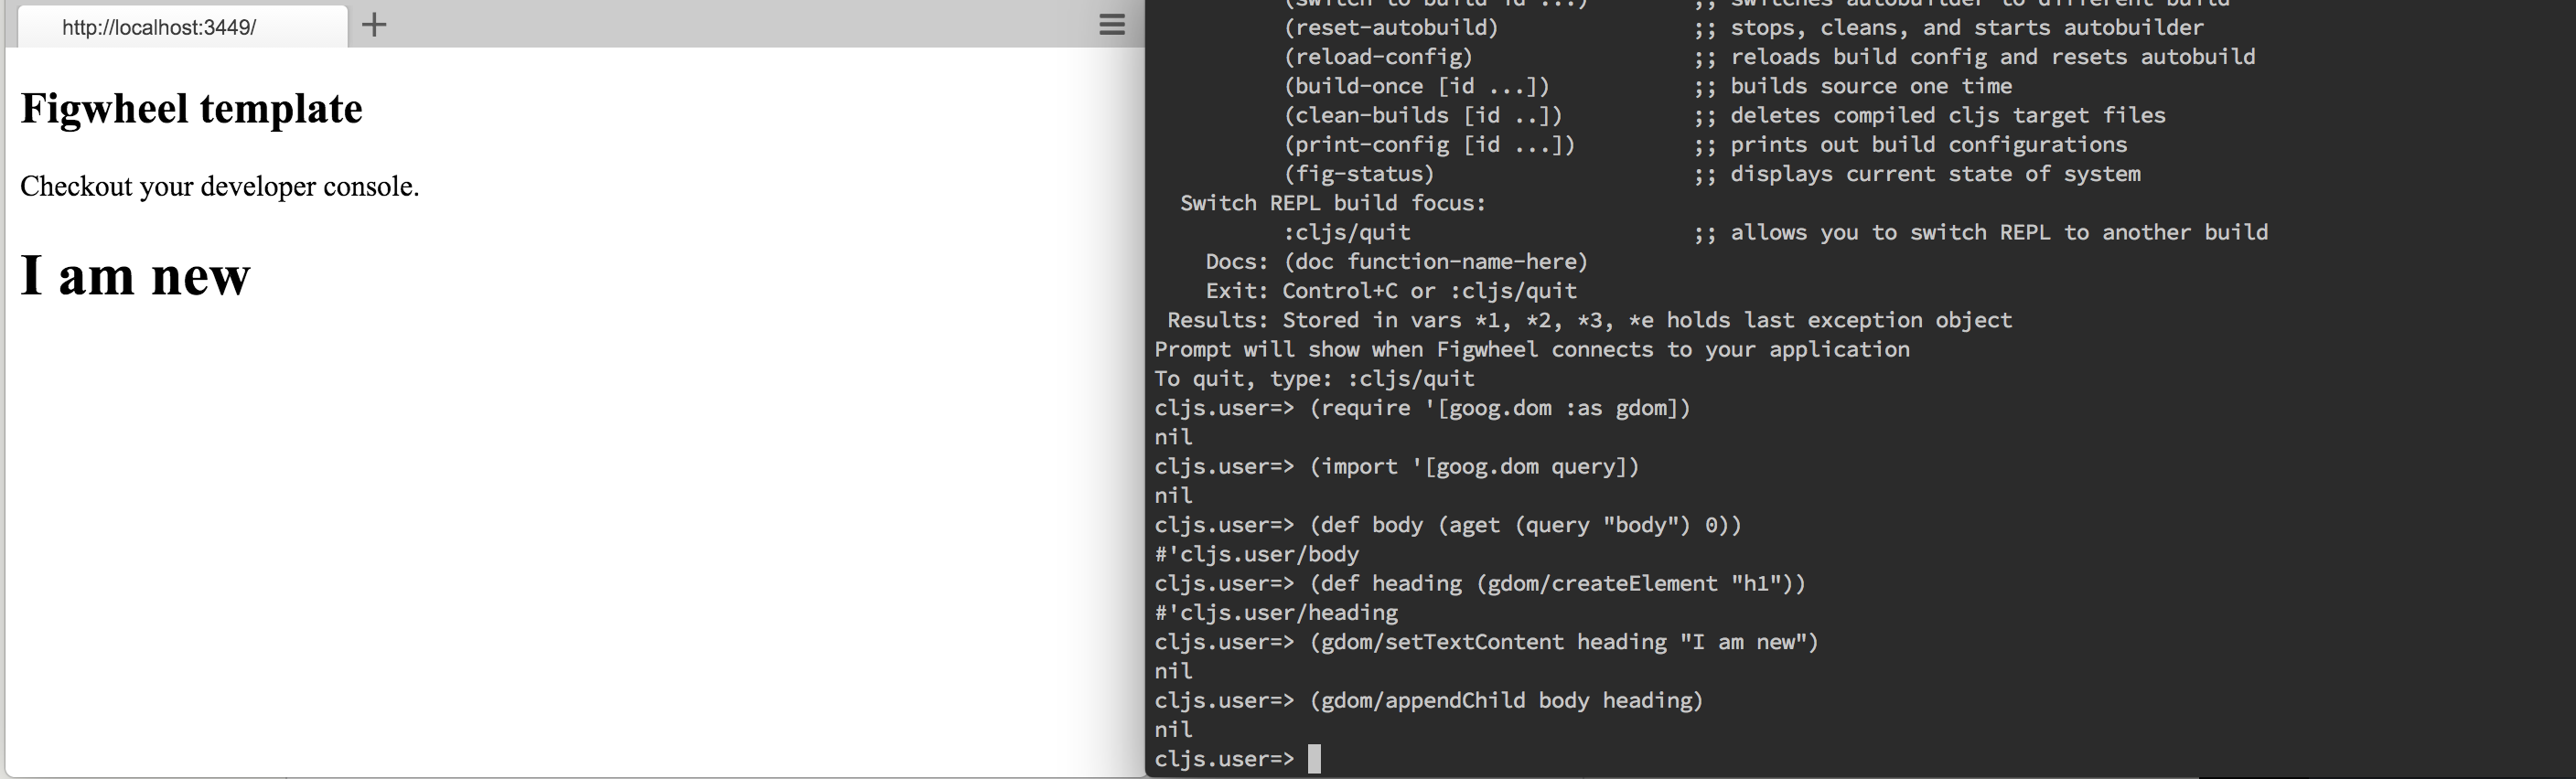
\includegraphics{lesson14/creating-dom-element.png}
\end{figure}

In order to add an element to the DOM, we'll use Google Closure's DOM
manipulation library to create an \texttt{h1} element, set its text
content, and append it to the end of the body. Let's walk through each
of these steps in the REPL.

\begin{lstlisting}[language=Clojure, caption={Creating a DOM element from the REPL}]
cljs.user=> (require '[goog.dom :as gdom])                 %\circled{1}%
nil

cljs.user=> (def body (.querySelector js/document "body")) %\circled{2}%
#'cljs.user/body

cljs.user=> (def heading (gdom/createElement "h1"))        %\circled{3}%
#'cljs.user/heading

cljs.user=> (gdom/setTextContent heading "I am new")
nil

cljs.user=> (gdom/appendChild body heading)                %\circled{4}%
nil
\end{lstlisting}

\begin{enumerate}[label=\protect\circled{\arabic*}]
\tightlist
\item
  Pull in the Google Closure Library that we need for DOM manipulation
\item
  Use the native DOM library to get the HTMLElement for the
  \texttt{\textless{}body\textgreater{}} tag and bind it to the
  \texttt{body} var
\item
  Use Google Closure to create a new element and give it some content
\item
  Append the element to the body of our page
\end{enumerate}

Since we are in unfamiliar territory, let's take a quick step back to
look at precisely what is going on, expression by expression.

\begin{lstlisting}[language=Clojure]
(require '[goog.dom :as gdom])
\end{lstlisting}

This expression loads all of the code in the \texttt{goog.dom}
namespace. This namespace contains a number of useful functions for
manipulating the DOM, and we will generally use this library instead of
vanilla JavaScript due to the fact that the \index{Google Closure Library}Closure Library normalizes
many browser quirks. This \texttt{require} makes the functions in this
namespace available under the alias, \texttt{gdom}. When calling code
that we have imported from another namespace, we use the form,
\texttt{(namespace/function\ args*)} Thus, we could call the
\texttt{getDocument()} function in this namespace as
\texttt{(gdom/getDocument)}.

\begin{lstlisting}[language=Clojure]
(def body (.querySelector js/document "body"))
\end{lstlisting}

Next, we use native JavaScript code to get a reference to the
\texttt{body} element. We do this by way of example to demonstrate that
DOM elements that we obtain with raw JavaScript are fully compatible
with the Google Closure Library.

\begin{lstlisting}[language=Clojure]
(def heading (gdom/createElement "h1"))
\end{lstlisting}

Next, we create an \texttt{h1} element and bind it to the var,
\texttt{heading}. At this point, the element is created but is not
attached to the DOM.

\begin{lstlisting}[language=Clojure]
(gdom/setTextContent heading "I am new")
\end{lstlisting}

Now we set the content of the detached \texttt{h1} node that we created.
Now that we have created the element and set its content appropriately,
we can append it to the document's body.

\begin{lstlisting}[language=Clojure]
(gdom/appendChild body heading)
\end{lstlisting}

This will append the DOM node that we have created as \texttt{heading}
to the document body, which we have bound to the \texttt{body} var. At
this point, the DOM is modified, and the web browser will reflect the
changes that we have made.

\subsection{You Try It}

\begin{itemize}
\tightlist
\item
  Using the example above as a reference, create a \texttt{p} tag with
  some content and append it to the body.
\item
  Use the \texttt{goog.dom.removeNode()} function to remove both the
  \texttt{h1} and \texttt{p} tags. Hint: this function takes the node to
  remove as its only parameter.
\end{itemize}

\subsubsection{Experiment}

Now that we have created an element, let's take the next step and
manipulate something that is already onscreen. Since we already have a
var containing the \texttt{HTMLElement} of the
\texttt{\textless{}h1\textgreater{}} tag that we created, let's change
the style on it and add a class. According to
the documentation
for \texttt{goog.dom}\footnote{https://google.github.io/closure-library/api/}, the \texttt{setProperties} function takes an
element and a JavaScript object mapping properties to values and applies
the properties to the DOM element.

\begin{lstlisting}[language=Clojure]
cljs.user=> (gdom/setProperties heading #js {"style" "color:red;"
                                             "class" "big-title"})
nil
\end{lstlisting}

We used the JavaScript object literal syntax that we learned about in
the last lesson to create a properties object. Then we called the
\texttt{goog.dom.setProperties()} function with the element whose
properties we wished to set and the properties object.

So far the process of manipulating the DOM is not dramatically different
from what we would do in JavaScript, albeit the parenthesis are in
different places, and we're using \texttt{def} instead of \texttt{var}.
Most of the time, we will not be working at a ``low level'' like this,
but we will use libraries like React to manage the DOM for us. However,
we need to build a solid foundational understanding before we can fully
take advantage of the higher-level technologies. Next, we will briefly
talk about getting user input and handling events before putting it all
together in a temperature conversion app.


\section{Getting User Input}

So far we have looked at the ``O'' side of ``I/O'', now we will turn to
getting user input. For now, we will look at extracting values from form
controls, since this is the most basic way to get data from users. As an
exercise, we will use a text input on the page and copy the value from
this input into another element. Instead of creating the entire DOM from
scratch, let's modify the project's \texttt{index.html} with the
structure that we want to work with. Be sure to reload your browser
after updating this file, since Figwheel does not replace the entire
HTML file on the fly.

\begin{lstlisting}[language=HTML, caption={resources/public/index.html}]
<!DOCTYPE html>
<html>
<head>
  <meta charset="UTF-8">
  <meta name="viewport" content="width=device-width, initial-scale=1">
  <link href="css/style.css" rel="stylesheet" type="text/css">
</head>
<body>
  <div id="app">                                         %\circled{1}%
    <div class="form-control">
      <label for="user-input">What do you say?</label>
      <input id="user-input" type="text" />
    </div>

    <p>You said, "<span id="copy-target"></span>". How mighty interesting.</p>
  </div>
                                                          %\circled{2}%
  <script src="cljs-out/dev-main.js" type="text/javascript"></script>
</body>
</html>
\end{lstlisting}

\begin{enumerate}[label=\protect\circled{\arabic*}]
\tightlist
\item
  Populate the \texttt{app} div with markup we will use to test I/O
\item
  Load the compiled ClojureScript
\end{enumerate}

Now the process for getting the text from the \texttt{user-input}
element is fairly straightforward. Once again, we will show the entire
REPL session then walk through each interesting piece of it. The result
will look like the following:

\begin{figure}[H]
\caption{Getting user input}
\centering
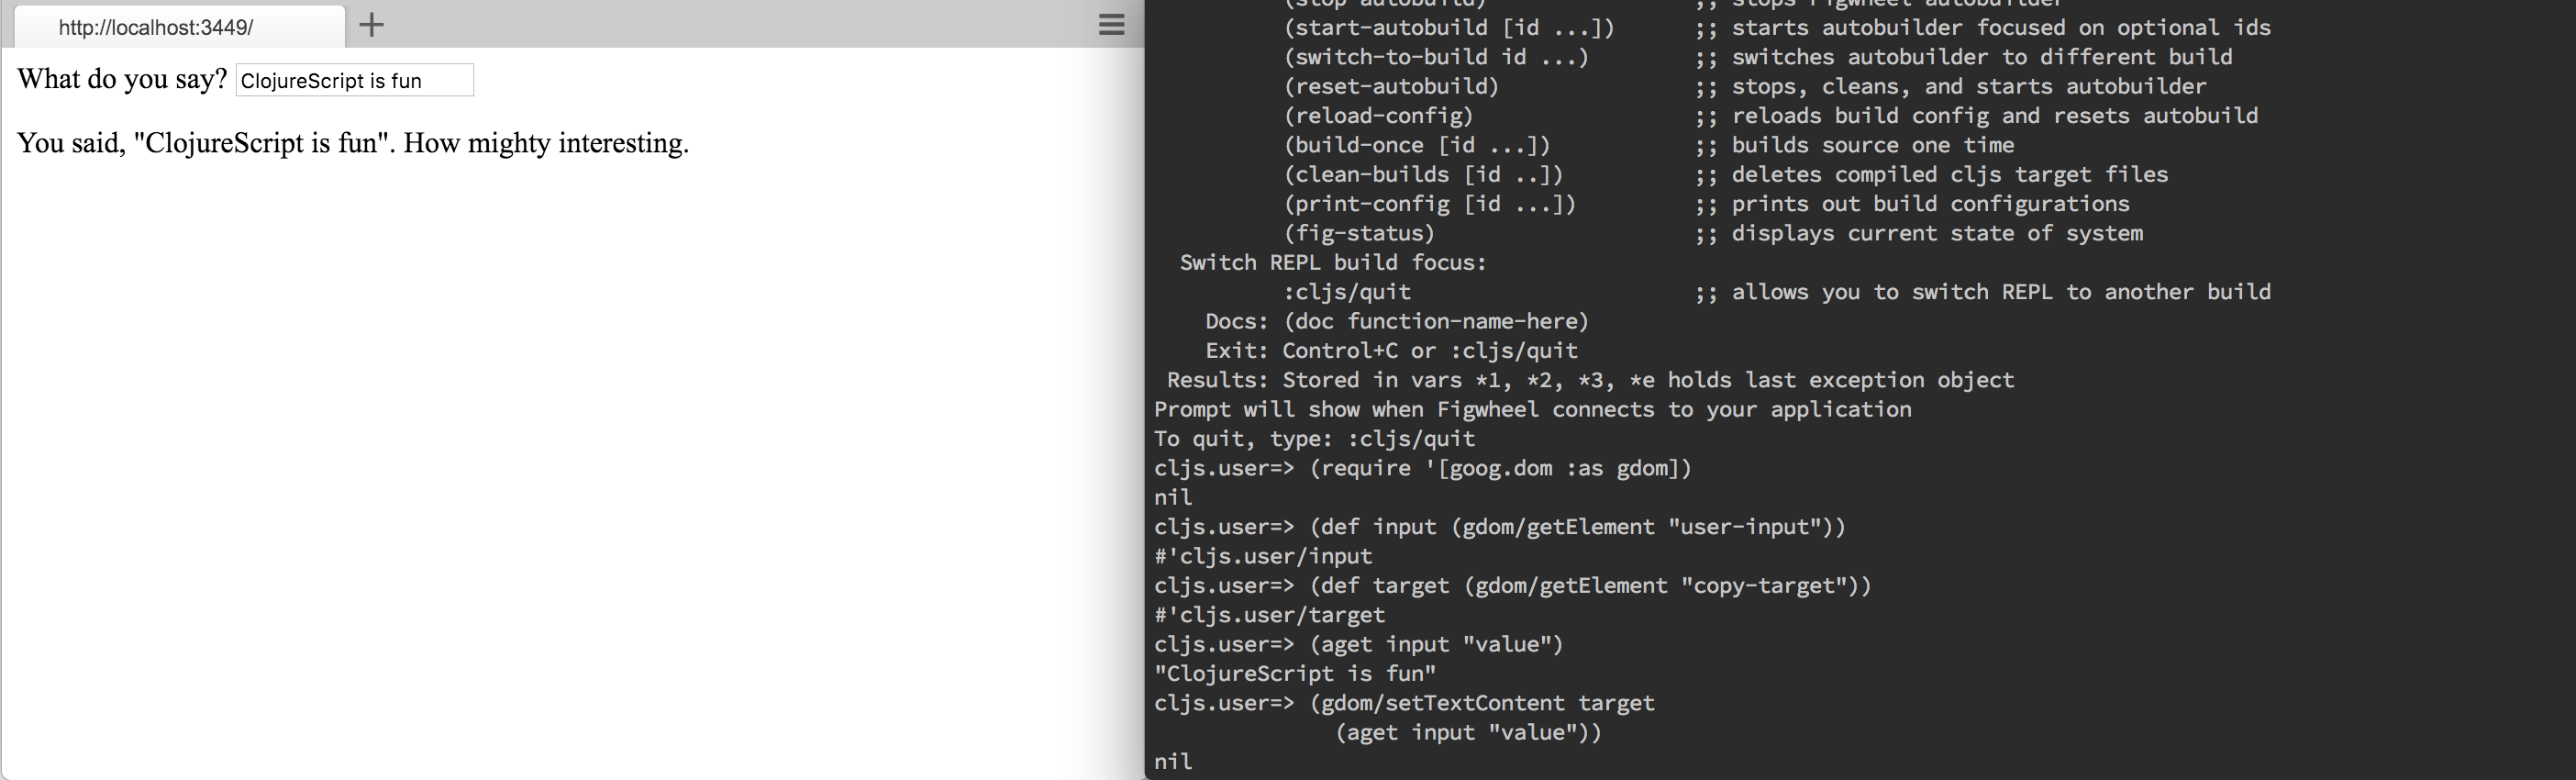
\includegraphics{lesson14/getting-input.png}
\end{figure}

\begin{lstlisting}[language=Clojure, caption={Reading the value of an input}]
cljs.user=> (require '[goog.dom :as gdom])
nil

cljs.user=> (def input (gdom/getElement "user-input"))
#'cljs.user/input

cljs.user=> (def target (gdom/getElement "copy-target"))
#'cljs.user/target

cljs.user=> (.-value input)                                %\circled{1}%
"ClojureScript is fun"

cljs.user=> (gdom/setTextContent target                    %\circled{2}%
              (.-value input))
nil
\end{lstlisting}

\begin{enumerate}[label=\protect\circled{\arabic*}]
\tightlist
\item
  \texttt{input} is a JavaScript object, so we can get its properties
  with property access syntax
\item
  Get the value of the input and update the target in one expression
\end{enumerate}

We have already discussed how \texttt{require} is used in this instance,
so we will move on to the next expression:

\begin{lstlisting}[language=Clojure]
(def input (gdom/getElement "user-input"))
\end{lstlisting}

Here, we use the \texttt{goog.dom.getElement()} function to retrieve the
input element by id. We could have accomplished the same thing with
native JavaScript as,
\texttt{(.getElementById\ js/document\ "user-input")}, but
\texttt{getElement} is more succinct. We do the same to get a reference
to the target element where we will output the text that we receive from
the user.

\begin{lstlisting}[language=Clojure]
(gdom/setTextContent target
  (.-value input))
\end{lstlisting}

In this expression, we get the \texttt{value} property of the input
element, which will contain whatever text the user has typed into it,
and update the text content of the target node with this value. This
code performs both the input (reading the input's \texttt{value}) and
output (writing the text content of the \texttt{target}).

Since we will not spend much time with low-level DOM manipulation, we
will not linger on this subject. If we ever find ourselves having to do
write DOM manipulation code, the Google Closure Library has excellent
documentation. Otherwise, do not be afraid to find a good ClojureScript
DOM library and use it!


\subsection{You Try It}

\begin{itemize}
\tightlist
\item
Include the dommy\footnote(https://github.com/plumatic/dommy) library and
go through the DOM manipulation examples again using Dommy instead of
Google Closure. You will need to add \emph{dommy} as a dependency to
\texttt{deps.edn} and restart Figwheel in order to start using dommy. Is
dommy easier to work with than goog.dom? Is there less boilerplate when
working with a ClojureScript library directly?
\end{itemize}

\section{Handling Events}

Closely related to getting user inputs is the issue of handling events.
We need triggers to tell us when something interesting has happened -
the user clicked a button, changed the value of a text input, etc. Once
again, we will use Google Closure libraries to create event handlers and
bind them to the DOM. We will extend the example of copying the value
from an input to another element, but this time, we will use an event to
update the target element every time the user types in the input.

\begin{lstlisting}[language=Clojure, caption={Using events to trigger updates}]
cljs.user=> (require '[goog.events :as gevents])
nil

cljs.user=> (defn update-target [evt]                      %\circled{1}%
              (gdom/setTextContent target
                (.. evt -currentTarget -value)))
#'cljs.user/update-target

cljs.user=> (gevents/listen input                          %\circled{2}%
                            "keyup"
                            update-target)
#object[Object [object Object]]
\end{lstlisting}

\begin{enumerate}[label=\protect\circled{\arabic*}]
\tightlist
\item
  Define a callback function that will be called on every event
\item
  Bind our event handler to the \texttt{keyup} event on the input
\end{enumerate}

Once more, let's take a moment to walk through this code to make sure we
can clearly grasp what is going on.

\begin{lstlisting}[language=Clojure]
(defn update-target [evt]
  (gdom/setTextContent target
    (.. evt -currentTarget -value)))
\end{lstlisting}

Here we create an event handler function that we intend to call on every
\texttt{keyup} event from the input. Notice that the inner portion of
this code looks very similar to the code that we manually entered in the
REPL. They both had the form,
\texttt{(gdom/setTextContent\ target\ value)}. The difference here is
that we are extracting the value from a JavaScript event rather than a
DOM element directly.

\begin{lstlisting}[language=Clojure]
(gevents/listen input "keyup" update-target)
\end{lstlisting}

\index{event handler}Finally, we use the \texttt{goog.events.listen()} function to attach an
event handler to the \texttt{input} element on the \texttt{keyup} event.
Now when we type in the input, the target element should instantly be
updated! We now have all of the pieces that we need to create the
temperature conversion app in the next lesson.


\subsubsection{Challenge}

Using the \texttt{goog.dom} and \texttt{goog.events} libraries, write an
app that does the following:

\begin{itemize}
\tightlist
\item
  Creates 2 password inputs (for password and password confirmation)
\item
  Creates a status text
\item
  Attaches listeners to the inputs so that the input values are compared
  every time a key is pressed
\item
  Sets the status text to ``Matches'' when the inputs are the same and
  ``Do not match'' when they differ.
\end{itemize}

Hint:

\begin{itemize}
\tightlist
\item
  Don't forget to get the \texttt{app} node to attach the children onto.
\item
  Bonus points if you do not disclose the typed text in the password
  fields
\end{itemize}

\emph{Possible Solution:}

\begin{lstlisting}[language=Clojure]
(ns passwords.core
  (:require [goog.dom :as gdom]
            [goog.events :as gevents]))

(defn values-same? [field-1 field-2]
  (= (aget field-1 "value")
     (aget field-2 "value")))

(defn handle-change [password confirmation status]
  (gdom/setTextContent status
                       (if (values-same? password confirmation)
                         "Matches"
                         "Do not match")))

(let [password (gdom/createElement "input")
      confirmation (gdom/createElement "input")
      status (gdom/createElement "p")
      app (gdom/getElement "app")]
  (gdom/setProperties password #js {"type" "password"})
  (gdom/setProperties confirmation #js {"type" "password"})

  (gevents/listen password "keyup"
                  #(handle-change password confirmation status))
  (gevents/listen confirmation "keyup"
                  #(handle-change password confirmation status))

  (gdom/setTextContent app "")
  (gdom/appendChild app password)
  (gdom/appendChild app confirmation)
  (gdom/appendChild app status))
\end{lstlisting}

\section{Summary}

In this lesson, we used both native JavaScript and Google Closure
Library code to get user input from a webpage and manipulate the DOM. We
also learned how to attach an event handler to an element so that we can
evaluate a callback in response to some action that the user takes. Now
that we have a way to interact with the user, we can begin creating much
more useful apps. We should now know how to:

\begin{itemize}
\tightlist
\item
  Require and use Google Closure Library functions
\item
  Create and manipulate DOM elements
\item
  Retrieve user input from the DOM
\item
  Attach event handlers to respond to user interactions
\end{itemize}

\chapter{Capstone 2 - Temperature Converter}

Over the past few lessons, we have learned the basic concepts that we
will need for practically any app that we write: variables for hanging
on to values that we want to re-use, control structures for determining
which code path should be taken, functions for defining re-usable
behavior and calculations, and I/O for interacting with the user. While
there is still much ground to cover, we can already begin to write
useful apps.

\begin{center}\rule{0.5\linewidth}{0.5pt}\end{center}

\textbf{In this lesson:}

\begin{itemize}
\tightlist
\item
  Create the structure of an app declaratively in HTML
\item
  Apply our knowledge of basic ClojureScript to create a widget-like app
\end{itemize}

\begin{center}\rule{0.5\linewidth}{0.5pt}\end{center}

In this lesson, we will build a simple app that will take the
temperature and convert it from Celsius to Fahrenheit or vice-versa,
depending on the value of a radio button that the user can toggle. For
this app, we will need an input for the user to enter a temperature, a
couple of radio buttons for them to select the unit of measure that they
have entered, and a target to display the converted value. This is what
the completed project looks like:

\begin{figure}[H]
\caption{Complete temp converter app}
\centering
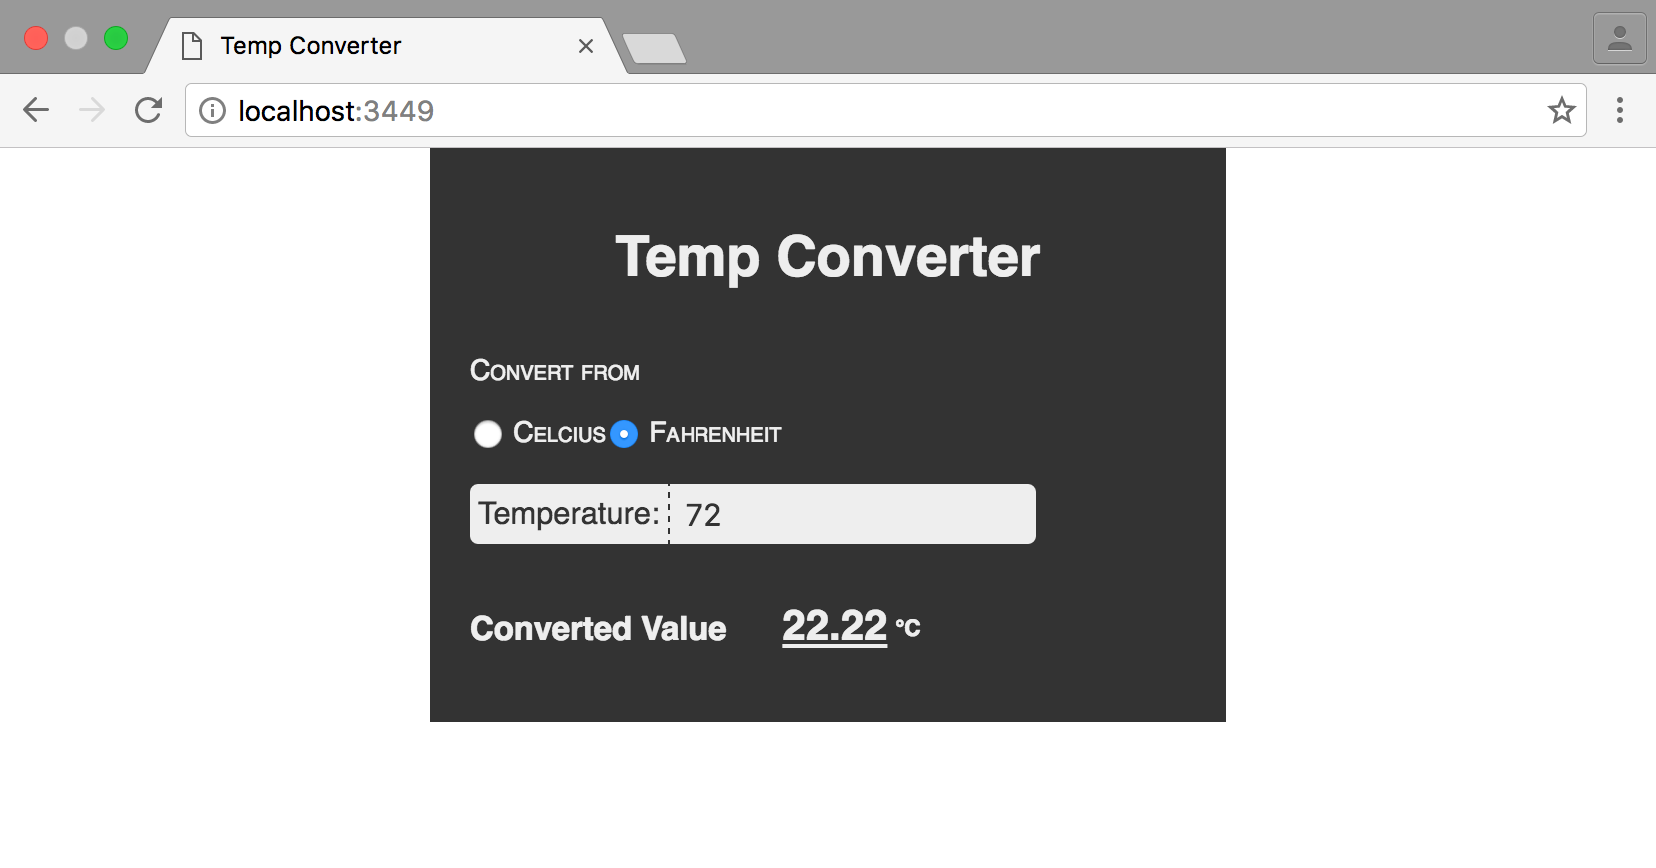
\includegraphics[width=10cm]{lesson15/temp-converter-screenshot.png}
\end{figure}

First, we will create the Figwheel project:

\begin{verbatim}
$ clj -X:new :template figwheel-main :name learn-cljs/temp-converter :args '["+deps"]'
\end{verbatim}

Again, since we will not be writing automated tests, remove the
\texttt{"test"} entry from \texttt{:watch-dirs} in
\texttt{dev.cljs.edn}.

\section{Creating the Markup}

In the last chapter, we manually built up the DOM, creating and
appending elements in code. Besides being cumbersome to work with, this
is not very idiomatic ClojureScript. Remember that we should favor
\emph{declarative} apps over \emph{imperative} ones. This time, we will
define our entire markup in HTML. Replace the \texttt{app} tag in the
generated \texttt{index.html} with the following.

\begin{lstlisting}[language=HTML, caption={Temperature converter markup}]
<div id="app">
  <h1>Temp Converter</h1>

  <div class="user-input">
    <div class="unit-control">                             %\circled{1}%
      <p>Convert from</p>
      <div class="radio-option">
        <input type="radio" id="unit-c" name="unit" value="c" checked="checked" />
        <label for="unit-c">Celsius</label>
      </div>
      <div class="radio-option">
        <input type="radio" id="unit-f" name="unit" value="f" />
        <label for="unit-f">Fahrenheit</label>
      </div>
    </div>

    <div class="temp-control">                             %\circled{2}%
      <label for="temp">Temperature:</label>
      <input type="number" id="temp" name="temp" />
    </div>
  </div>

  <div class="converted-output">                           %\circled{3}%
    <h3>Converted Value</h3>

    <span id="temp-out">-</span>
    <span id="unit-out">F</span>
  </div>
</div>
\end{lstlisting}

\begin{enumerate}[label=\protect\circled{\arabic*}]
\tightlist
\item
  Radio buttons used to switch between units
\item
  Text input for the user to enter a temperature
\item
  Result display area
\end{enumerate}

This markup defines all of the elements that we will use in our app, so
we do not need to worry about creating any ad-hoc DOM elements in our
code - we'll only deal with manipulating the elements that we have
already defined. Notice that we have given each element that we will be
interacting with a unique \texttt{id} attribute so that we can easily
get a reference to them using the \texttt{goog.dom/getElement} function.


\subsection{Quick Review}

\begin{itemize}
\tightlist
\item
  What is the advantage of structuring an app declaratively?
\item
  Before we write any ClojureScript code, list out the steps that are
  necessary to turn this static markup into an application
\end{itemize}


\section{Code Walkthrough}

Now we will write the ClojureScript code that will interact with the
webpage we just created and handle the business logic of converting
temperatures. To begin with, we will import the Google Closure libraries
that we have been using over the past few lessons: \texttt{goog.dom} for
DOM manipulation and \texttt{goog.events} for reacting to user input:

\begin{lstlisting}[language=Clojure]
(ns learn-cljs.temp-converter
  (:require [goog.dom :as gdom]
            [goog.events :as gevents]))
\end{lstlisting}

\index{bottom-up programming}ClojureScript is often written in a bottom-up fashion, in which we
define the low-level operations in our domain first and develop more
complex logic by combining the low-level operations. In this case, our
domain is very simple, but we will still define the business logic of
converting temperatures first:

\begin{lstlisting}[language=Clojure]
(defn f->c [deg-f]
  (/ (- deg-f 32) 1.8))

(defn c->f [deg-c]
  (+ (* deg-c 1.8) 32))
\end{lstlisting}

\index{DOM manipulation}Next, we want to get references to the important elements on the page.
We will use Google Closure to find DOM elements on the page and bind
each element to a var. This helps keeping the rest of the code clearer,
and it helps with performance, since we do not have the overhead of
searching the DOM every time we want to use one of these elements.

\begin{lstlisting}[language=Clojure]
(def celsius-radio (gdom/getElement "unit-c"))
(def fahrenheit-radio (gdom/getElement "unit-f"))
(def temp-input (gdom/getElement "temp"))
(def output-target (gdom/getElement "temp-out"))
(def output-unit-target (gdom/getElement "unit-out"))
\end{lstlisting}

Next, we will create a few functions that we will use in our event
handling code. As with any programming language, factoring each piece of
logic into its own function is considered good practice.

\begin{lstlisting}[language=Clojure]
(defn get-input-unit []
  (if (.-checked celsius-radio)
    :celsius
    :fahrenheit))

(defn get-input-temp []
  (js/parseInt (.-value temp-input)))

(defn set-output-temp [temp]
  (gdom/setTextContent output-target
                       (.toFixed temp 2)))
\end{lstlisting}

This code should look familiar, as we are dealing with the sort of DOM
manipulation that we have been performing over the past few lessons. The
\texttt{get-input-unit} and \texttt{get-input-temp} functions get the
unit of measure and temperature to convert respectively, and the
\texttt{set-output-temp} function updates the display element with the
converted temperature.

We will also need a function that we will use as an event handler any
time anything changes that will get the currently selected unit of
measure and temperature and will update the results section with the
converted temperature.

\begin{lstlisting}[language=Clojure]
(defn update-output [_]
  (if (= :celsius (get-input-unit))
    (do (set-output-temp (c->f (get-input-temp)))
        (gdom/setTextContent output-unit-target "F"))
    (do (set-output-temp (f->c (get-input-temp)))
        (gdom/setTextContent output-unit-target "C"))))
\end{lstlisting}

This function is the core of our app. It handles each event and updates
the UI accordingly. This function will be called with an event object as
an argument, but we follow a common convention of using an underscore to
name any parameter that we do not use. The other thing to note about
this code is that it uses \texttt{do} to group several expressions
together. \texttt{do} takes multiple expression, evaluates all of them
in order, and it evaluates to the value of the last expression. Thus,
the expression, \texttt{(do\ x\ y\ z)}, would evaluate \texttt{x} then
\texttt{y} then \texttt{z}, and the entire expression would have the
same value as just \texttt{z}. \index{side effects!within do@within\texttt{do}}This is useful if \texttt{x} and
\texttt{y} have side effects (in our case, updating DOM elements), but
we do not care what they evaluate to.


\subsection{You Try It}

\begin{itemize}
\tightlist
\item
  Add a button that will clear the temperature input
\end{itemize}

Finally, we will connect our logic to the UI by attaching the
\texttt{update-output} function as an \index{event handler}event handler whenever either
radio button is clicked or the input is updated. This will ensure that
any time the user changes anything that may affect the converted output,
we recalculate the results.

\begin{lstlisting}[language=Clojure]
(gevents/listen temp-input "keyup" update-output)
(gevents/listen celsius-radio "click" update-output)
(gevents/listen fahrenheit-radio "click" update-output)
\end{lstlisting}

There, in roughly 40 lines of code, we have a useful ClojureScript app!
For the sake of completeness, the entire code is printed below:

\begin{lstlisting}[language=Clojure, caption={learn\_cljs/temp\_converter.cljs}]
(ns learn-cljs.temp-converter
  (:require [goog.dom :as gdom]                            %\circled{1}%
            [goog.events :as gevents]))

(defn f->c [deg-f]                                         %\circled{2}%
  (/ (- deg-f 32) 1.8))

(defn c->f [deg-c]
  (+ (* deg-c 1.8) 32))

(def celsius-radio (gdom/getElement "unit-c"))              %\circled{3}%
(def fahrenheit-radio (gdom/getElement "unit-f"))
(def temp-input (gdom/getElement "temp"))
(def output-target (gdom/getElement "temp-out"))
(def output-unit-target (gdom/getElement "unit-out"))

(defn get-input-unit []                                     %\circled{4}%
  (if (.-checked celsius-radio)
    :celsius
    :fahrenheit))

(defn get-input-temp []
  (js/parseInt (.-value temp-input)))

(defn set-output-temp [temp]
  (gdom/setTextContent output-target
                       (.toFixed temp 2)))

(defn update-output [_]                                    %\circled{5}%
  (if (= :celsius (get-input-unit))
    (do (set-output-temp (c->f (get-input-temp)))
        (gdom/setTextContent output-unit-target "F"))
    (do (set-output-temp (f->c (get-input-temp)))
        (gdom/setTextContent output-unit-target "C"))))

(gevents/listen temp-input "keyup" update-output)          %\circled{6}%
(gevents/listen celsius-radio "click" update-output)
(gevents/listen fahrenheit-radio "click" update-output)
\end{lstlisting}

\begin{enumerate}[label=\protect\circled{\arabic*}]
\tightlist
\item
  Require the Google Closure modules needed for this app
\item
  Define conversion functions
\item
  Store each element that we will use in a var
\item
  Helper functions
\item
  Event handling callback
\item
  Attach event handler to \texttt{keyup} event in the temperature input
  and the click event on each radio button
\end{enumerate}


\subsection{Challenge}

This is a very simple app, and it could be extended quite easily. Here
are a couple of options for new features that you can add:

\begin{itemize}
\tightlist
\item
  Allow the user to select Kelvin as well, and perform the appropriate
  conversions.
\item
  Every time the code is reloaded, it will attach more event handlers.
  Use the initialization pattern discussed in Lesson
  6 to ensure that the event handlers are attached only once.
\end{itemize}


\section{Summary}

We will continue to acquire new building blocks that we will be able to
combine with what we have just learned to create more useful and
interesting applications. By now, we have a good feel for how
ClojureScript is structured, but so far we have not done much that
showcases ClojureScript's advantages over JavaScript. That is about to
change, as we begin to explore the areas that make ClojureScript unique.
In the next lessons, we will look at the rich collection data types that
make ClojureScript so productive.

\cleardoublepage
{\let\newpage\relax\part{Working With Data}}

In this section, we will get to know one of the most distinguishing
features of ClojureScript - its library of immutable collections and the
functions that operate on them. First, we will survey the collections
that ClojureScript offers as part of its standard library. Next, we will
study the \emph{sequence} abstraction that is one of the core
abstractions of the language. Then we will devote an entire lesson to
\emph{reduce}, the most general and powerful function that operates on
the sequence abstraction. We will finish this section by applying
ClojureScript's collection types to real-world domain modeling. For the
capstone, we will create a simple but functional contact book
application.

\begin{itemize}
\tightlist
\item Lesson 16: Grokking Collections
\item Lesson 17: Discovering Sequence Operations
\item Lesson 18: Summarizing Data
\item Lesson 19: Mastering Data With Maps and Vectors
\item Lesson 20: Capstone 3 - Contact Book
\end{itemize}

\chapter{Grokking Collections}

So far, we have been working with simple data types - strings, numbers,
keywords, and the like. We saw a few collections when we took our survey
of ClojureScript's syntax, but we glossed over exactly what they are and
how to use them in real applications. As we might imagine, writing
programs without any way to represent data that belongs together would
be cumbersome at best. JavaScript has arrays for representing lists of
things and objects for representing \emph{associative} data - that is,
data in which values are referred to by a specific string key, such as
the \texttt{title} and \texttt{content} of a blog post. We are probably
already familiar how these types of collections work from JavaScript or
another language.

\begin{center}\rule{0.5\linewidth}{0.5pt}\end{center}

\textbf{In this lesson:}

\begin{itemize}
\tightlist
\item
  Using lists for managing ordered data
\item
  Using maps for looking up values by a key
\item
  Using sets for keeping data unique
\end{itemize}

\begin{center}\rule{0.5\linewidth}{0.5pt}\end{center}


\subsection{Example: Contact Book}

It should come as no surprise that collections are a core feature of
ClojureScript - much more, in fact, than in most other languages. We
deal with collections every day. Take the example of a contact book
where we store details for friends and acquaintances. The contact book
itself is a collection of contact details, and each contact itself is a
collection of personal information.

\begin{figure}[H]
\caption{A contact book is a real-world collection}
\centering

\includegraphics[width=6cm]{lesson16/address-book.png}
\end{figure}

In JavaScript, we might model the contact book itself as a list and each
individual contact as an object with the properties, \texttt{name},
\texttt{address}, etc. It would probably look something like the
following:

\begin{lstlisting}[language=JavaScript, caption={Modeling a contact book in JavaScript}]
const contactBook = [                                      %\circled{1}%
    {
        name: "Phillip Jordan",
        address: "523 Sunny Hills Cir.",
        city: "Springfield",
        email: "phil.j@hotmail.com"
    },
    {                                                      %\circled{2}%
        name: "Clara Michaels",
        address: "4473 Point of the Pines",
        city: "Colorado Springs",
        email: null
    }
];
\end{lstlisting}

\begin{enumerate}[label=\protect\circled{\arabic*}]
\tightlist
\item
  Outer structure is an array for organizing a list of contacts
\item
  Inner structure is an object for describing a contact by a specific
  set of properties
\end{enumerate}

While we can effectively write programs using the arrays and objects
that JavaScript provides, ClojureScript gives us more focused tools, and
- more importantly - abstractions. In JavaScript, we can sort or filter
a list, and we can lookup a property on an object. They are different
data types that have essentially different behaviors. \index{collections}In ClojureScript,
there are multiple collection types that all conform to a specific
collection protocol. For those familiar with the concept of an
interface, all ClojureScript collections conform to a common interface.
That means that any code that is designed to work with a collection can
work with \emph{any} collection, whether that is a vector, set, list, or
map. We can then choose the specific collection type that we want to use
based on its performance characteristics and have confidence that we can
use the same familiar functions to operate on it. Not only that, but we
can implement the collection protocol in our own code, and ClojureScript
can operate on our own objects as if they were built into the language
itself.


\section{Defining Collections and Sequences}

Let's take a brief step back to define what a collection is and to take
a look at a closely related concept, the sequence. In ClojureScript, a
collection is simply any data type that holds more than one thing. It is
the opposite of a scalar, which represents only a single thing. Another
way to think of a collection is as a container for other data. \index{sequences}A
sequence, on the other hand, is a linear collection that has a beginning
and an end. All sequences are collections (because they are containers),
but not all collections are sequences.

\begin{figure}[H]
\caption{Collections and sequences}
\centering
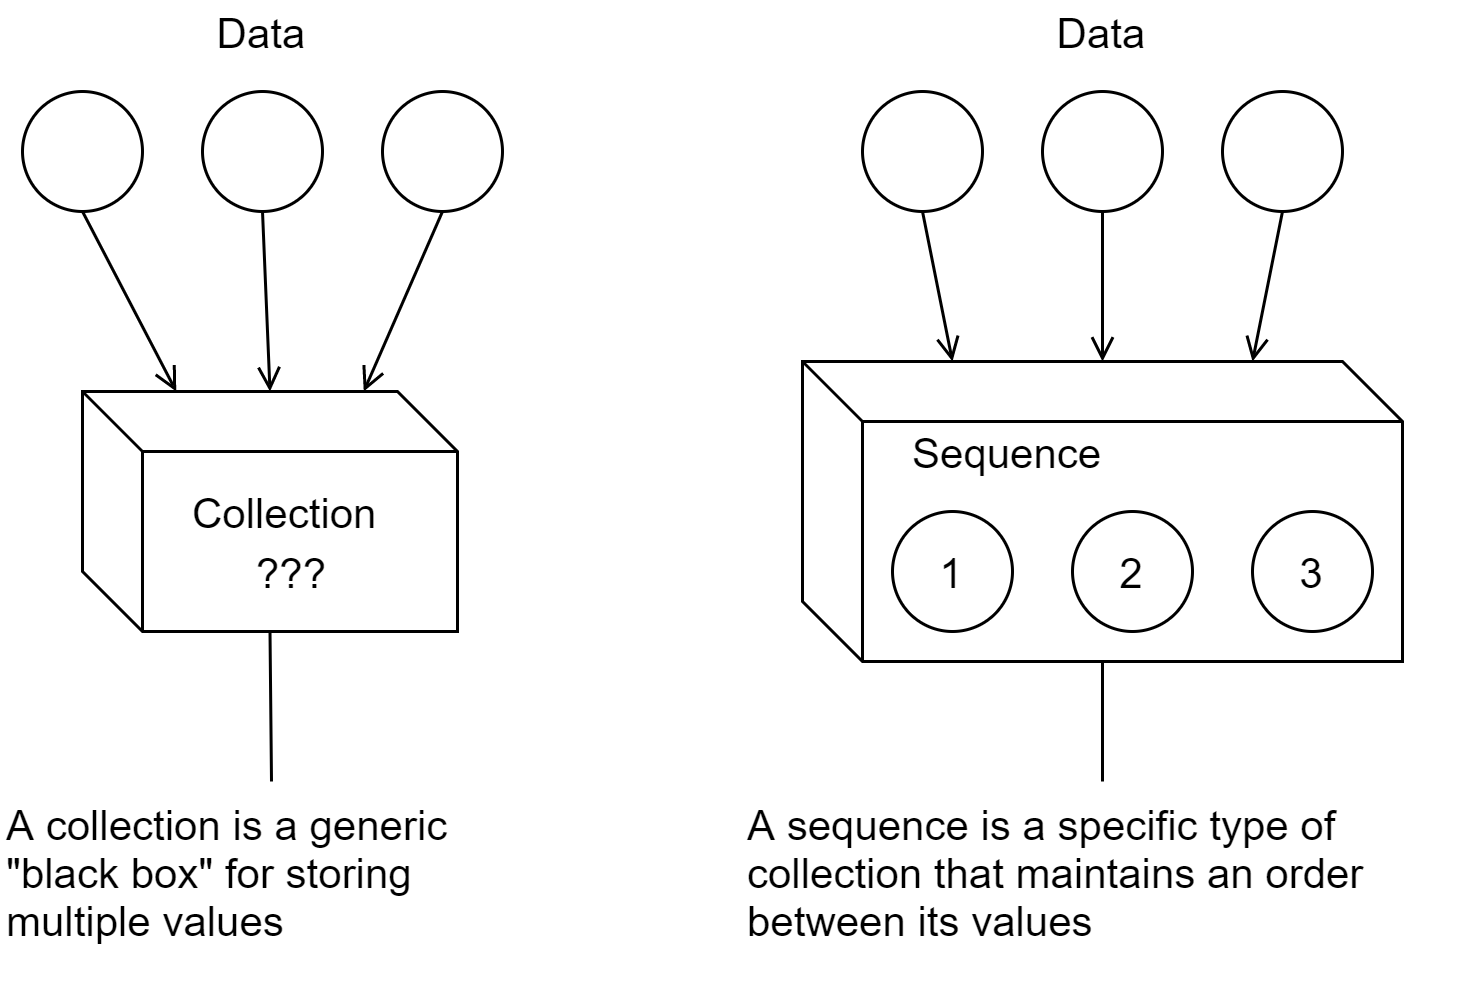
\includegraphics{lesson16/collections-and-sequences.png}
\end{figure}

In order for ClojureScript to treat something as a collection, it only
needs to be able to add something to it, and it does this by using the
oddly named \index{sequence operations!conj@\texttt{conj}}\texttt{conj} function (short for ``conjoin''). How that
something is added to the collection depends on the type of collection.
For instance, items are added to the beginning of a list but to the end
of a vector, and adding an item to a set only grows the set if the item
does not already exist. We can see an example of the behavior of
\texttt{conj} on different collections in the REPL.

\begin{lstlisting}[language=Clojure, caption={Using \texttt{conj} with different collections}]
cljs.user=> (conj '(:lions :tigers) :bears)                %\circled{1}%
(:bears :lions :tigers)

cljs.user=> (conj [:lions :tigers] :bears)                 %\circled{2}%
[:lions :tigers :bears]

cljs.user=> (conj #{:lions :tigers} :bears)                %\circled{3}%
#{:lions :tigers :bears}

cljs.user=> (conj #{:lions :tigers} :tigers)               %\circled{4}%
#{:lions :tigers}
\end{lstlisting}

\begin{enumerate}[label=\protect\circled{\arabic*}]
\tightlist
\item
  \texttt{conj} adds to the beginning of a list
\item
  \ldots{}or the end of a vector
\item
  A set has no order, so the new element is simply added to it
\item
  Adding an element that is already in a set has no effect
\end{enumerate}


\subsection{Quick Review: Collections}

\begin{itemize}
\tightlist
\item
  What is the only operation that we can be sure that \emph{every}
  collection will support?
\item
  Which collection type should we use to efficiently add to the
  beginning with \texttt{conj}?
\end{itemize}


\section{Sequences}

Sequences are a type of ClojureScript collection in which the elements
exist in some linear fashion. Whereas collections need only support
adding an element with \texttt{conj}, sequences must support 2
additional operations: \index{sequence operations!first@\texttt{first}}\texttt{first} and \index{sequence operations!rest@\texttt{rest}}\texttt{rest}. \texttt{first}
should return the first item in the sequence, and \texttt{rest} should
return another sequence with everything else. In the case that we have a
singleton sequence - that is, a sequence with only one element -
\texttt{rest} will evaluate to an empty sequence.

\begin{figure}[H]
\caption{First and rest of a sequence}
\centering
\includegraphics{lesson16/sequences-first-rest.png}
\end{figure}


This sequence abstraction seems quite intuitive - as long as we can get
the first bit of something an we can get another sequence with the
remaining bits, we can traverse the entire sequence, taking the first
bit off each time until nothing is left. Since the \texttt{rest} of a
sequence is another sequence, we can take the \texttt{first} element of
it until we finally get to the end. Keeping this in mind, we can create
a function that performs some sort of aggregation over a sequence by
repeatedly looping with the \texttt{rest} of a sequence until the
sequence is empty. For example, to add all the numbers in a sequence, we
could write the following function:

\begin{lstlisting}[language=Clojure, caption={Traversing a sequence}]
(defn add-all [xs]
  (loop [sum 0                                             %\circled{1}%
         nums xs]
    (if (empty? nums)                                      %\circled{2}%
      sum
      (recur (+ sum (first nums))
             (rest nums)))))                               %\circled{3}%
\end{lstlisting}

\begin{enumerate}[label=\protect\circled{\arabic*}]
\tightlist
\item
  Initialize the loop with a sum of \texttt{0} and all of the numbers
  that were given
\item
  When no numbers remain, return the sum that has been accumulated
\item
  When there are still numbers left in the sequence, loop again with the
  old sum plus the first number in the sequence as the new sum and the
  \texttt{rest} of the numbers as the new \texttt{nums}
\end{enumerate}

A visual will help us better understand what is going on here:

\begin{figure}[H]
\caption{Traversing a sequence}
\centering
\includegraphics{lesson16/sequence-traversing-with-first-and-rest.png}
\end{figure}

This process of repeatedly dividing a sequence between its
\texttt{first} and \texttt{rest} illustrates a core concept in
ClojureScript - sequence traversal. Thankfully, there is a rich library
of functions that work with sequences, so we seldom have to write such
tedious code as in the example above!

\subsection{Extra Credit}

\begin{itemize}
\tightlist
\item
  Look up the \texttt{reduce} function online. How could the add-all
  function be simplified using \texttt{reduce}?
\end{itemize}


\subsection{Quick Review: Sequences}

\begin{itemize}
\tightlist
\item
  In general, how would you get the \emph{nth} element of a sequence
  using only the \texttt{first} and \texttt{rest} function?
\item
  What is the \texttt{first} of an empty list?
\item
  What is the \texttt{rest} of an empty list?
\end{itemize}

\begin{notice}[title={It's all about abstraction}]
Several JavaScript libraries - most notably \emph{lodash}\index{lodash} and
\emph{Ramda}\index{Ramda} - have similar functions that can get the first element and
the rest of the elements from an array. The key difference between these
libraries' sequence functions and ClojureScript's sequences is that
sequences are an \emph{abstraction} that are not intrinsically tied to
any data type. If it looks like a sequence, then to ClojureScript, it is
one. After getting used to programming to abstractions, JavaScript's
data types start to feel a bit rigid like, well, concrete.  
\end{notice}

\section{Using Lists for Sequential Data}

Lists are one of the simplest data types in ClojureScript. They are
sequences that can hold other objects of any type that can efficiently
be accessed starting at the beginning and progressing linearly. Lists
are most often used in two cases: first, when we have a collection of
data that will always be accessed from beginning to end, and second,
when we want to treat some data as a stack where the last item added is
the first one to retrieve. Lists, however, are not efficient for random
access (i.e.~getting the \emph{nth} element in the sequence).

\text{data types!lists}There are two ways to create a list in ClojureScript. The first is with
the \texttt{list} function, and the second is using the literal syntax,
\texttt{\textquotesingle{}()}. As collections, lists support adding
elements with \texttt{conj}; and as sequences, they support
\texttt{first} and \texttt{rest}.

\begin{lstlisting}[language=Clojure, caption={Working with lists}]
cljs.user=> (list 4 8 15 16 23 42)                         %\circled{1}%
(4 8 15 16 23 42)

cljs.user=> '(4 8 15 16 23 42)                             %\circled{2}%
(4 8 15 16 23 42)

cljs.user=> (conj '(:west :north :north) :south)           %\circled{3}%
(:south :west :north :north)

cljs.user=> (first '("Tom" "Dick" "Harry"))                %\circled{4}%
"Tom"

cljs.user=> (rest '("Tom" "Dick" "Harry"))
("Dick" "Harry")
\end{lstlisting}

\begin{enumerate}[label=\protect\circled{\arabic*}]
\tightlist
\item
  Creating a list with the \texttt{list} function
\item
  Creating a list with the literal syntax
\item
  Prepending to a list with \texttt{conj}
\item
  Treating a list as a sequence with \texttt{first} and \texttt{rest}
\end{enumerate}


\section{Using Vectors for Indexed Data}

\index{data types!vectors}While lists are useful in some applications, vectors are much more
widely used in practice. Think of vectors as the (immutable)
ClojureScript counterpart of JavaScript's array. They are a very
versatile collection that can be traversed sequentially like a list or
accessed by 0-based index. Unlike a list, \texttt{conj} adds elements to
the \emph{end} of a vector. For collections where we may want to get a
specific element or extract a specific slice, a vector is usually the
best choice.

\begin{lstlisting}[language=Clojure, caption={Working with vectors}]
cljs.user=> (conj ["Moe" "Larry"] "Curly")                 %\circled{1}%
["Moe" "Larry" "Curly"]

cljs.user=> (first ["Athos" "Porthos" "Aramis"])
"Athos"

cljs.user=> (rest ["Athos" "Porthos" "Aramis"])            %\circled{2}%
("Porthos" "Aramis")

cljs.user=> (nth ["Athos" "Porthos" "Aramis"] 1)           %\circled{3}%
"Porthos"

cljs.user=> (["Athos" "Porthos" "Aramis"] 1)               %\circled{4}%
"Porthos"
\end{lstlisting}

\begin{enumerate}[label=\protect\circled{\arabic*}]
\tightlist
\item
  \texttt{conj} adds to the end of a vector
\item
  \texttt{rest} always returns a sequence
\item
  \texttt{nth} looks up a specific element by index
\item
  Vectors themselves are functions that can look up an element when
  given an index as an argument
\end{enumerate}

We discovered a couple of interesting properties of vectors and
sequences in the REPL session above. First, we see that when we applied
the \texttt{rest} function to a vector, we did not get a vector back.
Instead, what we got looked like a list but is in fact a generic
sequence that acts much like a list. Since vectors are optimized for
indexed access, ClojureScript performs some coercion whenever we use
them as sequences. While this makes little difference most of the time,
it is good to be aware of. Second, we see that in ClojureScript, vectors
are functions that expect as their argument the index of an element to
look up. That is why we could evaluate,
\texttt{({[}"Athos"\ "Porthos"\ "Aramis"{]}\ 1)}. Interestingly, almost
everything in ClojureScript can be used as a function - vectors, maps,
keywords, and symbols can all be used as functions (although if we do
not give them the arguments that they require, we may get unexpected
results).

We will be working with vectors a great deal, since their performance
characteristics are appropriate in many real-world scenarios.


\section{Using Maps for Associative Data}

\index{data types!maps}Maps are an incredibly useful collection that allow us to map keys to
arbitrary values. They are the ClojureScript analog of JavaScript's
object, but they are much simpler. Whereas JavaScript objects can have
functions attached to them with complex rules (and some might say dark
magic) surrounding what \texttt{this} refers to, maps are simply data.
There is nothing preventing the use of a function as a value in the map,
but that does not create any binding between the function and the map.

We can think of a map as a post office. Anyone who has a mailbox is
assigned a specific number that they can use to find their mail. When
the post office receives mail for a specific customer, they put that
mail in the box that is associated with that customer. Essentially, the
post office maintains an association between a box number and the mail
belonging to a single customer. Likewise, maps maintain an association
between some identifying \emph{key} and some arbitrary \emph{value}.

Maps can be created either with the literal syntax, \texttt{\{\}}, or
with the \texttt{hash-map} function.

\begin{lstlisting}[language=Clojure, caption={Creating maps}]
cljs.user=> {:type "talk"                                  %\circled{1}%
             :title "Simple Made Easy"
             :author "Rick Hickey"}
{:type "talk", :title "Simple Made Easy", :author "Rick Hickey"}

cljs.user=> (hash-map :foo "bar", :baz "quux")             %\circled{2}%
{:baz "quux", :foo "bar"}
\end{lstlisting}

\begin{enumerate}[label=\protect\circled{\arabic*}]
\tightlist
\item
  The common way to create a map is to alternate keys and values inside
  curly braces
\item
  Maps can also be created with the \texttt{hash-map} function, which
  takes alternating keys and values
\end{enumerate}

When using maps as a collection with \texttt{conj} or as a sequence with
\texttt{first} and \texttt{rest}, the behavior may not be intuitive.
ClojureScript allows us to treat a map as a sequence of
\texttt{{[}key,\ value{]}} pairs, so when we want to add a map entry
with \texttt{conj}, we append it as a vector containing a key and a
value.

\begin{lstlisting}[language=Clojure]
cljs.user=> (conj {:x 10 :y 12} [:z 7])
{:x 10, :y 12, :z 7}
\end{lstlisting}

Similarly, if we take the \texttt{first} of a map, we will get some map
entry as a \texttt{{[}key,\ value{]}} pair, and if we take the
\texttt{rest}, we will get a sequence of such pairs. Knowing about this
behavior will help us in the next lesson when we discuss the common
functions used to operate on sequences.

\begin{lstlisting}[language=Clojure]
cljs.user=> (first {:x 10, :y 12, :z 7})
[:x 10]

cljs.user=> (rest {:x 10, :y 12, :z 7})
([:y 12] [:z 7])
\end{lstlisting}

One other advantage of ClojureScript maps over JavaScript objects is
that any value may be used as the key - not just strings. For instance,
if we were creating a Battleship-like game, we could use a vector of
grid coordinates as keys.

\begin{lstlisting}[language=Clojure]
cljs.user=> {[:b 3] :miss, [:a 7] :hit}
{[:b 3] :miss, [:a 7] :hit}
\end{lstlisting}

While we can use any value as a key, keywords are most commonly used
because of their convenient syntax and because they also act as
functions that can look up the map entry associated with themselves in a
map. This is an extremely common idiom in ClojureScript and one that
will be used extensively throughout this book. Additionally, maps may
also be used as functions (surprise!) that can look up the value
associated with the key given as the argument.

\begin{lstlisting}[language=Clojure]
cljs.user=> (def fido {:breed "Boxer" :color "brown" :hungry? true})
#'cljs.user/fido

cljs.user=> (get fido :breed)
"Boxer"

cljs.user=> (:color fido)
"brown"

cljs.user=> (fido :hungry?)
true
\end{lstlisting}

We have seen that there are quite a few usage patterns for dealing with
maps. This is by no means a comprehensive reference, and we will
continue to see more ways to work with maps in later lessons.

\subsection{You Try It}

\begin{itemize}
\tightlist
\item
  What happens when you try to \texttt{conj} an element onto a map when
  that map already has a value for the key of the new element,
  e.g.~\texttt{(conj\ \{:flavor\ "Mint"\}\ {[}:flavor\ "Chocolate"{]})}?
\item
  As we just saw, ClojureScript treats a map as a collection of
  \texttt{{[}key\ value{]}} pairs. Knowing this, how might we add an
  entry to the following map such that we set a \texttt{:price} of
  \texttt{12.99}?
\end{itemize}

\begin{lstlisting}[language=Clojure]
(conj {:title "Kneuter Valve", :part-num 5523} ...)
\end{lstlisting}


\section{Using Sets for Unique Data}

\index{data types!sets}A set in ClojureScript resembles a mathematical set, which can contain
any number of elements, but they must be unique. Sets are often used for
de-duplicating data in some other collection or for checking whether a
piece of data is contained in the set.

\begin{lstlisting}[language=Clojure, caption={Working with sets}]
cljs.user=> (def badges
                 #{:quick-study :night-owl :neat-freak})   %\circled{1}%
#'cljs.user/badges

cljs.user=> (contains? badges :night-owl)                  %\circled{2}%
true

cljs.user=> (conj badges :quick-study)                     %\circled{3}%
#{:quick-study :neat-freak :night-owl}

cljs.user=> (conj badges :clojurian)                       %\circled{4}%
#{:quick-study :neat-freak :night-owl :clojurian}

cljs.user=> (first badges)                                 %\circled{5}%
:quick-study
\end{lstlisting}

\begin{enumerate}[label=\protect\circled{\arabic*}]
\tightlist
\item
  Creating a set using the literal syntax, \texttt{\#\{\ ...\ \}}
\item
  \texttt{contains?} is often used with sets and checks for membership
\item
  \texttt{conj} is a no-op if the element is already a member of the set
\item
  \texttt{conj} adds a new member if it is unique
\item
  We can treat a set as a sequence, although the order of elements is
  arbitrary
\end{enumerate}

While sets are not used as often as vectors and maps, they are
incredibly useful when dealing with unique values.


\subsection{Quick Review}

\begin{itemize}
\tightlist
\item
  Which collection should be used to represent each of the following: a
  product on an e-commerce site, a news feed, tags attached to a blog
  post?
\item
  Using the Clojure(Script) documentation, find:

  \begin{itemize}
  \tightlist
  \item
    Additional functions that can be used with maps
  \item
    Additional functions that can be used with sets
  \end{itemize}
\item
  Explain in your own words the difference between a collection and a
  sequence.
\end{itemize}


\section{Summary}

This was a long lesson, but a crucial one in our understanding of
ClojureScript. One of the key features of the language is its rich
collection library, but in order to wield this library effectively, we
must first have a grasp on the collections available to us. We have
learned:

\begin{itemize}
\tightlist
\item
  How the collection library is based around two abstract types - the
  collection and the sequence
\item
  How sequence functions are built on top of the \texttt{first} and
  \texttt{rest} functions
\item
  What data structures are built into ClojureScript and how they are
  used
\end{itemize}

Over the next few lessons, we will apply the collection library to some
common UI programming problems, culminating in a contact book
application.

\chapter{Discovering Sequence Operations}

\index{sequence operations}Programming is all about abstractions. The entire field of software
engineering is devoted to making programs and systems that are better
for human beings to reason about and maintain. The key to making clear
and accurate systems is found in the concept of abstraction, which is
identifying patterns that recur often and generalizing them to something
that is more widely applicable. We humans are quite adept at abstracting
concepts. In fact, it is one of the first skills that we learn in
childhood. Imagine a toddler who calls every fruit that they see,
``apple'', because they are familiar with an apple and have identified a
number of similarities between it and other fruits. Eventually, this
child will learn that there is a whole class of distinct but similar
objects called ``fruit'', each of which has its own unique properties
yet shares many other properties with every other thing that we call
fruit. The idea of abstraction in programming is very similar: we see a
number of different constructs that appear similar in many ways, yet
each of which are distinct from the rest, and we must determine how to
appropriately generalize the properties that each construct shares in
common.

\begin{center}\rule{0.5\linewidth}{0.5pt}\end{center}

\textbf{In this lesson:}

\begin{itemize}
\tightlist
\item
  Apply a transformation to every element in a sequence
\item
  Efficiently convert between sequence types
\item
  Filter sequences to only specific elements
\end{itemize}

\begin{center}\rule{0.5\linewidth}{0.5pt}\end{center}


\subsection{Example: Calculating Sales Tax}

Imagine that we are writing an e-commerce shopping cart app. One of the
requirements is that we display the sales tax for each item in the cart
as well as a summary section with the total price and the total sales
tax. We will learn to apply a couple of ClojureScript's sequence
operations to solve this problem.

\begin{figure}[H]
\caption{A shopping cart}
\centering
\includegraphics{lesson17/priming-example-shopping-cart.png}
\end{figure}

\section{The Sequence Abstraction}

As we have seen in the previous lesson, ClojureScript has identified
collections as an important general abstraction. The collection
abstraction had the single operation, \texttt{conj}, for ``adding'' an
item into the collection. The important point to remember is that each
specific collection type defines what it means for an item to be added
to it, and adding to a list, a vector, a set, or a map, could have a
different effect in each case. This is where the power behind
abstraction comes into play - we can write code in a general way, using
abstract operations like \texttt{conj} with the confidence that it will
work regardless of the concrete data type that we work with. While
collections are the most general abstraction in ClojureScript,
\emph{sequences} are a narrower, more focused abstraction. Sequences
allow us to think about data that can be considered linearly, which will
be perfect for the products in this shopping cart example.

Sequences are a core abstraction in many of the domains that we as web
developer work in. Whether it is a feed of blog posts, an email inbox,
or a series of financial transactions, most applications have one or
more sequences of data at their core. When we approach these types of
programs from an object-oriented approach\index{object-oriented programming}, we usually think first about
the individual objects in the system and what behaviors they support.
For instance, in the case of an email program, we might be inclined to
start by creating a \texttt{Message} object with messages like
\texttt{markRead()} or \texttt{getLabels()}. Once we have modeled these
objects, we might build some sort of collection object to put them in,
or we may just use an array and iterate over it. The ClojureScript way
is a little different (and simpler). Instead of focusing on the
individual behaviors of each granular object, we begin by thinking about
the collective properties such as, ``Which messages are read?'', or
``How many messages are in the inbox?''

Let's take a step back and consider how we can think about the shopping
cart problem in terms of sequences. First, we can model the cart as a
vector of line items where each line item is a map with a \texttt{:name}
and \texttt{:price} key.

\begin{lstlisting}[language=Clojure, caption={Modeling a shopping cart}]
cljs.user=> (def cart [{:name "Silicone Pancake Mold" :price 10.49}
                       {:name "Small Pour-Over Coffee Maker" :price 18.96}
                       {:name "Digital Kitchen Scale" :price 24.95}])
#'cljs.user/cart
\end{lstlisting}

There are two properties that we need to know about this sequence. First,
we need to know how to calculate sales tax for each item in the
sequence, and second, we need to know how to sum all of the prices and
all of the sales taxes. The general problems here are applying some
operation to each element in a sequence and summarizing values from
across a sequence into a single value. We can solve these problems with
the functions \index{sequence operations!map@\texttt{map}}\texttt{map} and \texttt{reduce}, respectively.


\section{Transforming With Map}

The \texttt{map} function takes a sequence and returns a new sequence in
which every element corresponds to an element in the original sequence
with some function applied to it. For instance, we can map the function
\texttt{inc} - which gets the increment of an integer - over a list of
numbers to get a new sequence in which each element is the increment of
the corresponding number in the original sequence.

\begin{lstlisting}[language=Clojure]
cljs.user=> (map inc '(100 200 300))
(101 201 301)
\end{lstlisting}

When we mapped the \texttt{inc} function over the list,
\texttt{(100\ 200\ 300)}, the result was a new list,
\texttt{(101,\ 201,\ 301)}. Each number in this new list is the
increment of each element in the original list. You can imagine
\texttt{map} as walking over a sequence, and as it comes to each
element, it takes that element, passes it through a function, and puts
the result into a new sequence. In this case, it applied \texttt{inc} to
\texttt{100} and put the result, \texttt{101} into the new sequence. It
did the same with the second and third elements, transforming
\texttt{200} to \texttt{201} and \texttt{300} to \texttt{301}. Finally,
the call to \texttt{map} returned the list of all of the transformed
numbers.

\begin{figure}[H]
\caption{A concrete \texttt{map} example}
\centering
\includegraphics{lesson17/map-concrete-example.png}
\end{figure}

In general, \texttt{map} takes some function, \texttt{f}, and some
sequence and returns a new sequence whose elements are the result of
applying \texttt{f} to each element in the original sequence. Keep in
mind that \texttt{map} returns a \emph{new sequence}, so the original
sequence is not touched. When the problem that we are working with
involves any sort of a transformation of a sequence, \texttt{map} is
usually the first tool that we should turn to. Many of the times that we
would use a \texttt{for} loop in another language, we can use
\texttt{map} in ClojureScript.

\begin{figure}[H]
\caption{A general \texttt{map} example}
\centering
\includegraphics{lesson17/map-general-example.png}
\end{figure}


\subsection{Quick Review}


Take a look at the following code snippet:

\begin{lstlisting}[language=Clojure]
(def samples [[8 12 4]
              [9 3 3 6]
              [11 4]])

(def result-1 (map first samples))

(def result-2 (map dec result-1))
\end{lstlisting}

\begin{itemize}
\tightlist
\item
  What is the value of \texttt{result-1}?
\item
  What is the value of \texttt{result-2}?
\item
  What is the value of \texttt{samples}?
\item
  How would you get a collection with the length of each vector inside
  \texttt{samples}?
\end{itemize}


\subsection{Adding Sales Tax With Map}

Coming back to our initial example of adding sales tax to a shopping
cart, we will use \texttt{map} to create a new cart where each item is
like an item in the original cart, but with the addition of a
\texttt{:sales-tax} key. If we were using JavaScript, this would be an
obvious case for a for loop, similar to the code below:

\begin{lstlisting}[language=JavaScript, caption={Adding sales tax imperatively with JavaScript}]
const taxRate = 0.079;
const cart = [                                             %\circled{1}%
    { name: "Silicone Pancake Mold", price: 10.49 },
    { name: "Small Pour-Over Coffee Maker", price: 18.96 },
    { name: "Digital Kitchen Scale", price: 24.95 },
];

for (let item  of cart) {                                  %\circled{2}%
    item.salesTax = item.price * taxRate;
}
\end{lstlisting}

\begin{enumerate}[label=\protect\circled{\arabic*}]
\tightlist
\item
  Define a cart as a list of products with a \texttt{name} and
  \texttt{price}
\item
  Loop over every product in the cart, adding a new \texttt{salesTax}
  property
\end{enumerate}

This code should feel very familiar for JavaScript programmers, as it
just loops over an array and updates each element in-place. We updated
the \texttt{cart} array in-place, which may have had an unintended
consequence in some other part of the code that uses this array or any
of the individual objects that it contains. What looked like a simple
and innocuous piece of code could actually be the source of subtle bugs
down the road.

We can use \texttt{map} to write a solution in ClojureScript (or
JavaScript) that - in addition to being more concise - is simpler and
less error-prone. Remember that \texttt{map} takes two arguments: a
function to apply to each individual element, and a sequence. We already
have a simple model of a shopping cart that we will use, so all that we
need is a function to apply to each cart item that will produce a new
item with sales tax added. Mapping this function over our shopping cart
then becomes a one-liner.

\begin{lstlisting}[language=Clojure, caption={Adding sales tax with ClojureScript}]
cljs.user=> (def tax-rate 0.079)
#'cljs.user/tax-rate

cljs.user=> (defn add-sales-tax [cart-item]                %\circled{1}%
              (let [{:keys [price]} cart-item]
                (assoc cart-item :sales-tax (* price tax-rate))))
#'cljs.user/add-sales-tax

cljs.user=> (add-sales-tax {:name "Medium T-Shirt"         %\circled{2}%
                            :price 10.00})
{:name "Medium T-Shirt", :price 10, :sales-tax 0.79}

cljs.user=> (map add-sales-tax cart)                       %\circled{3}%
({:name "Silicone Pancake Mold", :price 10.49, :sales-tax 0.8287100000000001}
 {:name "Small Pour-Over Coffee Maker", :price 8.96, :sales-tax 0.70784}
 {:name "Digital Kitchen Scale", :price 24.95, :sales-tax 1.97105})
\end{lstlisting}

\begin{enumerate}[label=\protect\circled{\arabic*}]
\tightlist
\item
  Define a function that transforms an item without sales tax into an
  item with sales tax
\item
  Test this function on a single item
\item
  Map this transformation over the entire cart to get a new cart with
  sales tax added
\end{enumerate}

The meat of this code is in the add-sales-tax function, which takes a
single cart item and returns an item with sales tax. One of the most
important aspects of creating maintainable code is choosing good names,
so we use a \texttt{let} expression to name the price of the item passed
in simply \texttt{price}. On the next line, we use the \texttt{assoc}
function to create a new map that is like \texttt{cart-item} but with
the addition of one more entry whose key is \texttt{:sales-tax} and
whose value is \texttt{(*\ price\ tax-rate)}. \texttt{assoc} is an
incredibly useful utility function that allows us to add or update a
\index{associative collections}specific entry in an \emph{associative} collection - that is, a
collection that has the concept of \emph{keys} that are associated with
a \emph{value}, most commonly maps. We pass \texttt{assoc} a collection
(in this case, \texttt{cart-item}), the key that we wish to set, and the
value to set it to, and the result is a new collection with the
appropriate entry added or updated.

Next, we test this function on a single cart item to ensure that it
works as expected. This test could be copied almost verbatim into a unit
test suite to protect against regressions, but we will save that for
another lesson. Finally, we get the result that we want with one simple
expression: \texttt{(map\ add-sales-tax\ cart)}. This expression reads
almost like English, ``Map the `sales-tax' function over the `cart'
sequence.'' There are no array indexes to maintain, no possibility of
off-by-1 errors, overwriting variables, or unintended consequences of
mutating \texttt{cart}. The solution, like all ClojureScript strives to
be, is simple and concise.


\subsection{You Try It}

Now that we have seen how map works, let's write some code to perform
various transformations to the product list.

\begin{itemize}
\tightlist
\item
  Write a \texttt{map} expression that returns a sequence of only the
  names of the products (hint: the \texttt{:name} keyword acts as a
  function that looks up the \texttt{:name} key in a map.
\item
  Write a \texttt{discount} function that takes a list of products and a
  percent amount to deduct from the price of each product and returns a
  sequence of discounted products. You can fill in this template as a
  starting point:
\end{itemize}

\begin{lstlisting}[language=Clojure]
(defn discount [products pct-discount]
  (map (fn [product] ...) products))
\end{lstlisting}


\section{Coercing Results With Into}

\index{sequence operations!into@\texttt{into}}There is one final ``gotcha'' that we need to be aware of with map and
other sequence operations. As we can see in this example, \texttt{cart}
is a vector, but the result of the call to \texttt{map} was something
that looked like a list. That is no mistake - \texttt{map},
\texttt{filter}, and other sequence functions commonly accept any type
of sequence as input but return a general data structure called a seq as
a result. \index{data types!seq}A seq is a general sequence type that behaves similarly to a
list. When we build up a pipeline of functions to pass some sequence
through, we generally don't care about what data type is produced at
each step, since we rely on the sequence abstraction to treat a vector
in the same way as a list and a list in the same way as a seq, etc. A
common ClojureScript idiom is to use the \texttt{into} function to
convert a seq back into the type that we want afterwards:

\begin{lstlisting}[language=Clojure, caption={Coercing a seq}]
cljs.user=> (def my-vec ["Lions" "Tigers" "Bears" "Lions"])
#'cljs.user/my-vec

cljs.user=> (defn loud [word]
              (str word "!"))
#'cljs.user/loud

cljs.user=> (map loud my-vec)                              %\circled{1}%
("Lions!" "Tigers!" "Bears!" "Lions!")

cljs.user=> (into [] (map loud my-vec))                    %\circled{2}%
["Lions!" "Tigers!" "Bears!" "Lions!"]

cljs.user=> (into '() (map loud my-vec))                   %\circled{3}%
("Lions!" "Bears!" "Tigers!" "Lions!")

cljs.user=> (into #{} (map loud my-vec))                   %\circled{4}%
#{"Lions!" "Tigers!" "Bears!"}
\end{lstlisting}

\begin{enumerate}[label=\protect\circled{\arabic*}]
\tightlist
\item
  Mapping yields a seq
\item
  The seq can be put into a new vector
\item
  Putting the seq into a list reverses the elements
\item
  Putting the seq into a set de-duplicates it
\end{enumerate}

\texttt{into} takes a destination collection and a source collection and
\emph{conjoins} every element in the destination collection to the
source collection. It walks over the source sequence one element at a
time, using the same semantics as the \texttt{conj} function to add each
element to the destination sequence. Since \texttt{conj} adds to the end
of a vector but the beginning of a list, this explains why the elements
in the resulting list is reversed. This pattern of coercing sequences
with \texttt{into} is extremely common in ClojureScript, and we will use
it extensively in later lessons.


\subsection{Quick Review}

As we have just learned, \texttt{into} repeatedly applies \texttt{conj}
to add each element from some sequence into a collection. We need to be
familiar with how \texttt{conj} works with different collections in
order to understand the results of into.

\begin{itemize}
\tightlist
\item
  Re-write the following expression as a series of calls to
  \texttt{conj}: \texttt{(into\ {[}{]}\ \textquotesingle{}(:a\ :b\ :c))}
\item
  What is the result of
  \texttt{(conj\ (conj\ (conj\ \textquotesingle{}()\ 1)\ 2)\ 3)}
\item
  What would change if we replaced the empty list,
  \texttt{\textquotesingle{}()} in the previous exercise with an empty
  vector, \texttt{{[}{]}}?
\end{itemize}


\section{Refining With Filter}

\index{sequence operations!filter@\texttt{filter}}We can now transform one sequence into another with \texttt{map}. There
are many problems that we can solve with just this one tool, but
consider the case where we don't want to consider \emph{every} element
in a sequence - for instance, we are only interested in processing
taxable items or users over the age of 21 or addresses in the state of
Vermont. In these cases, \texttt{map} will not suffice, since map always
produces a new sequence in which each element has a 1-to-1
correspondence to an element in the original sequence. This is where
\texttt{filter} comes into play. Whereas we use map to transform a
sequence in its entirety, we use filter to narrow down a sequence to
only the elements that we are interested in.

The \texttt{filter} function is fairly straightforward and similar to
JavaScript's \texttt{Array.prototype.filter()} function. It takes a
function, \texttt{f}, and a sequence, \texttt{xs} and returns a new
sequence of only the elements for which \texttt{(f\ x)} returns a truthy
value. Again, this is one of those functions that is much easier to
understand once we see it in action.

\begin{lstlisting}[language=Clojure, caption={Filtering a sequence}]
cljs.user=> (filter even? '(1 2 3 4 5))                    %\circled{1}%
(2 4)

cljs.user=> (defn longer-than-4? [s]                       %\circled{2}%
              (> (count s) 4))
#'cljs.user/longer-than-4?

cljs.user=> (filter longer-than-4?                         %\circled{3}%
                    ["Life" "Liberty" "Pursuit" "of" "Happiness"])
("Liberty" "Pursuit" "Happiness")
\end{lstlisting}

\begin{enumerate}[label=\protect\circled{\arabic*}]
\tightlist
\item
  Filter a sequence with a standard library function
\item
  Define a predicate (a function that returns a boolean) to use with
  filter
\item
  Filter using the function we just defined
\end{enumerate}

We can think of \texttt{filter} as inspecting the original sequence and
only allowing certain elements through to the new sequence. It is kind
of like a bouncer who enforces certain rules to determine who has
access. If any element does not meet the criteria, they're out! In the
first example, we gave \texttt{filter} the criteria function (often
called a \index{predicate function}\emph{predicate}), \texttt{even?}, and a list of numbers. It
checked each number in the list against the function \texttt{even?} and
built up a new sequence from only the even numbers. This process is
illustrated below:

\begin{figure}[H]
\caption{Applying filter to a sequence}
\centering
\includegraphics{lesson17/applying-filter.png}
\end{figure}

In the second example, we pass a function that we created to filter, but
the process is exactly the same. The length of each string that we pass
in is checked, and only words that exceed four characters are in the
filtered sequence.


\subsection{Finding Taxable Items With Filter}

With this knowledge of how \texttt{filter} operates, it is simple to get
only the taxable items from the shopping cart. First, we'll update our
cart model to include a \texttt{:taxable?} key on each item.

\begin{lstlisting}[language=Clojure]
cljs.user=> (def cart [{:name "Silicone Pancake Mold" :price 10.49 :taxable? false}
                       {:name "Small Pour-Over Coffee Maker" :price 18.96 :taxable? true}
                       {:name "Digital Kitchen Scale" :price 24.95 :taxable? true}])
#'cljs.user/cart
\end{lstlisting}

Now let's take a first pass at filtering the list to only the taxable
items.

\begin{lstlisting}[language=Clojure]
cljs.user=> (defn is-taxable? [item]
              (get item :taxable?))
#'cljs.user/is-taxable?

cljs.user=> (filter is-taxable? cart)
({:name "Small Pour-Over Coffee Maker", :price 18.96, :taxable? true}
 {:name "Digital Kitchen Scale", :price 24.95, :taxable? true})
\end{lstlisting}

Three lines of code (including the predicate function) to filter a
sequence is not bad. Even better, there is no \texttt{for} loop in
sight, which means that there is no room for off-by-one errors. This is
pretty concise, but in ClojureScript, there is usually a way to make
things more concise. Remember that keywords can be used as functions
that look themselves up in a map. That means that if we call,
\texttt{(:taxable?\ \{:name\ "Small\ Pour-Over\ Coffee\ Maker"\ :price\ 18.96\ :taxable?\ true\})},
it will look up the \texttt{:taxable?} key in the map,
\texttt{\{:name\ "Small\ Pour-Over\ Coffee\ Maker"\ :price\ 18.96\ :taxable?\ true\}},
yielding \texttt{true}. This means that our \texttt{is-taxable?}
function is redundant and can be replaced with just the keyword,
\texttt{:taxable?}.

\begin{lstlisting}[language=Clojure]
cljs.user=> (filter :taxable? cart)
({:name "Small Pour-Over Coffee Maker", :price 18.96, :taxable? true}
 {:name "Digital Kitchen Scale", :price 24.95, :taxable? true})
\end{lstlisting}

We just accomplished filtering the list with a 1-liner that is every bit
as clear as the previous version and is far simpler than the JavaScript
alternative. Now we can really start to appreciate the simplicity that
is so highly prized in the ClojureScript community.


\subsubsection{Challenge}

Data manipulation is one of ClojureScript's strongest suits, but it does
not serve much use until we somehow present it to the users of our
system. Create a ClojureScript file that defines a shopping cart and
renders a list of the name, price, and tax of every \emph{taxable}
product that it contains. One possible solution is below.

\begin{lstlisting}[language=Clojure, caption={Rendering a shopping cart}]
(ns shopping-cart.core
  (:require [goog.dom :as gdom]))

(def tax-rate 0.079)
(def cart [{:name "Silicone Pancake Mold" :price 10.49 :taxable? false}
           {:name "Small Pour-Over Coffee Maker" :price 18.96 :taxable? true}
           {:name "Digital Kitchen Scale" :price 24.95 :taxable? true}])

(defn add-sales-tax [cart-item]
  (assoc cart-item
         :sales-tax (* (:price cart-item) tax-rate)))

(def taxable-cart
  (map add-sales-tax
       (filter :taxable? cart)))

(def item-list (gdom/createDom "ul" nil ""))

;; Helper function to generate the display text for a product
(defn display-item [item]
  (str (:name item)
       ": "
       (:price item)
       " (tax: "
       (.toFixed (:sales-tax item) 2)
       ")"))

;; Create the list of products
(doseq [item taxable-cart]
  (gdom/appendChild
   item-list
   (gdom/createDom "li" #js {} (display-item item))))

;; Clear the entire document and append the list
(gdom/removeChildren (.-body js/document))
(gdom/appendChild (.-body js/document) item-list)
\end{lstlisting}


\section{Summary}

In this lesson, we started to feel the power of programming using the
high-level sequence abstraction. We learned that most of the places
where we would use a \texttt{for} loop in JavaScript can be expressed
more clearly and concisely with a sequence operation. Finally we put
this knowledge to use in creating a shopping cart component that renders
items in a cart with sales tax. The operations that we looked at in this
lesson all took a sequence in and evaluated to a new sequence. In the
next lesson, we will look at another useful class of problems that take
a sequence in and evaluate to a scalar value.


\chapter{Summarizing Data}

So far we have learned some useful operations that we can perform over
sequences:

\begin{itemize}
\tightlist
\item
  \texttt{map} for transforming each element
\item
  \texttt{filter} for selecting certain elements
\item
  \texttt{into} for converting between collection types
\end{itemize}

There is a lot that we can do with just these few functions. In fact, we
rarely need to use something like a \texttt{for} loop with these
functions at our disposal. In the last lesson, we used these functions
to calculate sales tax for items in a shopping cart and filter to only
the taxable items. However, consider the scenario where we would like to
get the total price of the cart or the average value of items in the
cart. In this case, we cannot use map - we want a single value, and map
always evaluates to another sequence the same size as the original.
Filter is also obviously not what we are looking for. Is there some way
to get ``summary'' data from out of a sequence without resorting to
\texttt{for} loops? There are indeed other options, the most common of
which is the \texttt{reduce} function.

\begin{center}\rule{0.5\linewidth}{0.5pt}\end{center}

\textbf{In this lesson:}

\begin{itemize}
\tightlist
\item
  Aggregating values over an entire sequence
\item
  Writing reducing functions
\item
  Simplifying recursive code with \texttt{reduce}
\end{itemize}

\begin{center}\rule{0.5\linewidth}{0.5pt}\end{center}


\subsection{Exercise: Getting cart value}

Let's take the same general shopping cart model from the last lesson and
try to find the total value of every item in the cart. We will again
consider an example of how we could do this imperatively in JavaScript.
This time, we are going on a space journey and need to pick up a couple
of supplies that we may need on the way:

\begin{lstlisting}[language=JavaScript, caption={Imperative shopping cart value}]
const cart = [                                             %\circled{1}%
    { name: "Tachyon Emitter Array", price: 1099.45 },
    { name: "Dilithium Matrix", price: 2442.00 },
    { name: "Antimatter Chamber Sealant Rings (4)", price: 19.45 },
    { name: "Toothbrushes (2-pack)", price: 8.50 }
];

let total = 0;                                             %\circled{2}%
for (let item of cart) {
    total += item.price;
}

console.log(total.toFixed(2)); // "3569.40"
\end{lstlisting}

\begin{enumerate}[label=\protect\circled{\arabic*}]
\tightlist
\item
  Use the same cart data structure that we used in the
  previous lesson
\item
  Calculate a running total with a \texttt{for} loop
\end{enumerate}

The pattern here is easy to see: we have some value - in this case the
variable, \texttt{total} that is updated for every element in the
\texttt{cart} array. We see and use code like this on a daily basis, so
it is not hard to figure out what is going on, but there is unnecessary
complexity in the for loop. \index{reduce}In ClojureScript, the pattern that we will
use is a \texttt{reduce}.

\begin{lstlisting}[language=Clojure]
cljs.user=> (def cart                                      %\circled{1}%
              [{:name "Tachyon Emitter Array" :price 1099.45}
               {:name "Dilithium Matrix" :price 2442.00}
               {:name "Antimatter Chamber Sealant Rings (4)" :price 19.45}
               {:name "Toothbrushes (2-pack)" :price 8.50}])
#'cljs.user/cart

cljs.user=> (defn add-price [total item]                   %\circled{2}%
              (+ total (:price item)))
#'cljs.user/add-price

cljs.user=> (def total (reduce add-price 0 cart))          %\circled{3}%
#'cljs.user/total

cljs.user=> (.toFixed total 2)
"3569.40"
\end{lstlisting}

\begin{enumerate}[label=\protect\circled{\arabic*}]
\tightlist
\item
  Define the cart data structure
\item
  Create a reducing function that takes a running total and a new
  element and yields a new total
\item
  Apply this reducing function to the entire cart to extract the total
\end{enumerate}


\section{Understanding Reduce}

\index{sequence operations!reduce@\texttt{reduce}}While the workings of \texttt{map} and \texttt{filter} were evident just
looking at some code that uses them, we need to dig a little deeper with
\texttt{reduce}. Like \texttt{map} and \texttt{filter}, it takes a
function and a sequence and returns \emph{something}. However,
\texttt{reduce} also takes an extra parameter, and the function that it
takes looks a little different than the functions that we passed to
\texttt{map} and \texttt{filter}. For one thing, this function takes two
parameters instead of just one. It also does not always return a
sequence. So then, how does \texttt{reduce} work?

Reduce commonly takes three parameters: an initial value, a reducing
function, and a sequence. It first evaluates the reducing function with
the initial value and the first element of the sequence as its arguments
and takes the evaluated value and passes it into the reducing function
again, along with the second item of the collection. It continues
evaluating the reducing function for each element in the sequence,
feeding the resulting value back into the next call. Finally,
\texttt{reduce} itself evaluates to whatever the final call to the
reducing function yields. This it quite a lot to wrap our heads around,
so let's use a diagram to help us understand visually what is going on.

\begin{figure}[H]
\caption{Reducing over a sequence}
\centering
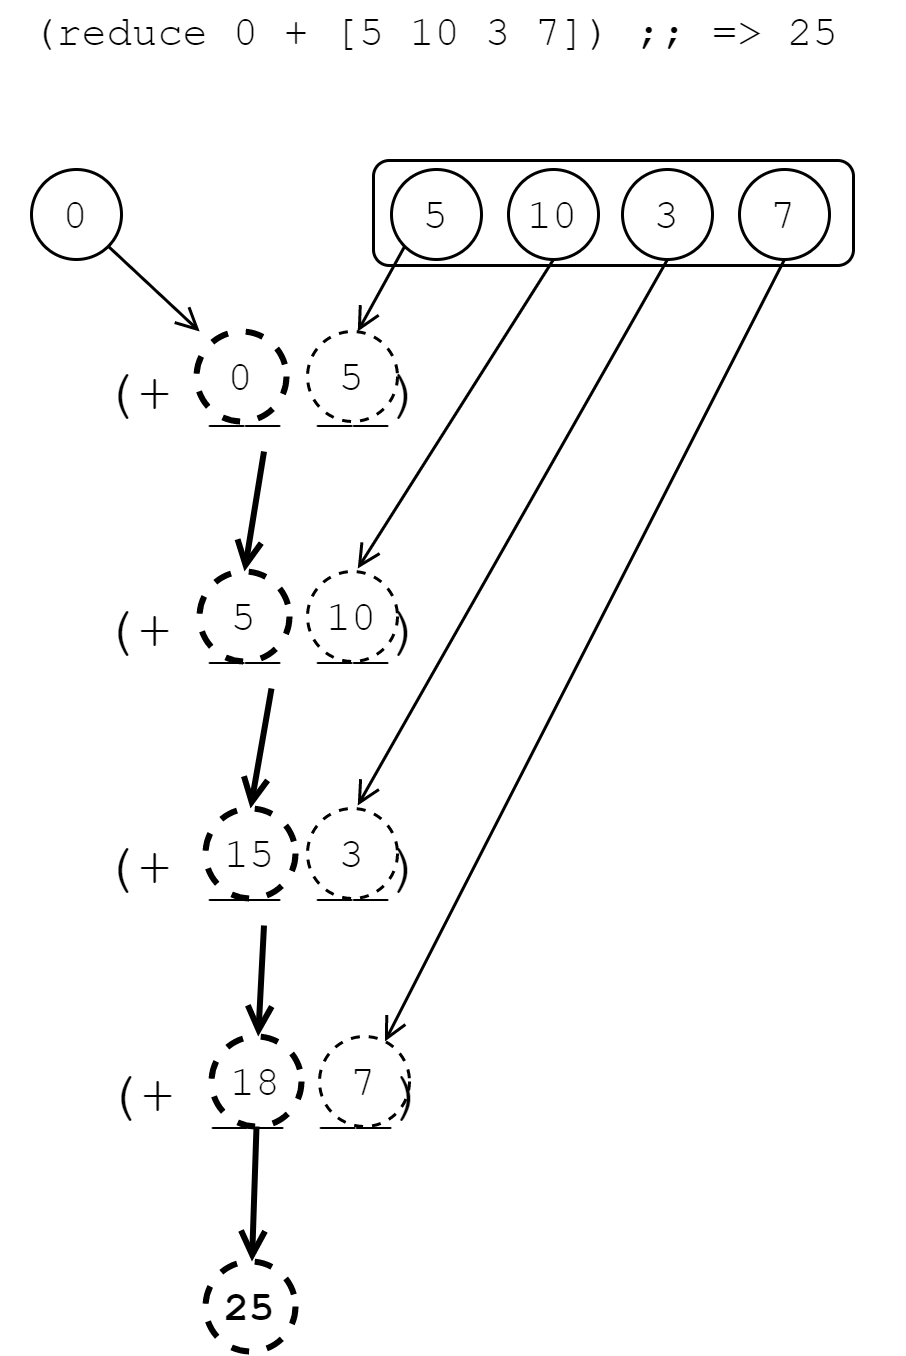
\includegraphics{lesson18/reduce-over-sequence.png}
\end{figure}

We can see that reduce keeps building up a value over each evaluation of
the reducing function. On the first call, it added the initial value,
\texttt{0} and the first element of the sequence, \texttt{5}, to get
\texttt{5}. It then added this value and the next element in the
sequence, \texttt{10}, to get \texttt{15}. It proceeded through the
entire sequence in this manner and yielded the last value, \texttt{25},
as the final result. Notice that we were able to take a function that
does not know how to operate on a sequence (\texttt{+}) and somehow
applied it to get the sum of all of the numbers in a sequence.

\index{accumulator}Imagine children packing snowballs for a snowball fight: they hold a
little bit of snow in one hand and pack on more snow with their other
hand. Every time they pack on more snow, the snowball grows larger and
larger, until the snowball is to their liking. Reduce operates in a very
similar way, ``accumulating'' more and more data with each pass. For
this reason, the first parameter that is passed to the reducing function
is often called an \emph{accumulator} or a \emph{memo}.


\subsection{Quick Review}

Given the following code:

\begin{lstlisting}[language=Clojure]
;; Create a seq of words
(def words (clojure.string/split
            "it was the best of times it was the worst of times"
            #" "))

(defn count-words [counts word]
  (update-in counts [word] #(inc (or %\%% 0))))

(def word-counts (reduce count-words {} words))
\end{lstlisting}

\begin{itemize}
\tightlist
\item
  What is the data type of \texttt{word-counts}?
\item
  What is the value of \texttt{word-counts}?
\end{itemize}

Before trying this code out at the REPL, use a pencil and paper to write
out the calls that will be made to the \texttt{count-words} function. If
you need to look up documentation on a specific function that is
unfamiliar, you can either call \texttt{(doc\ function-name)} from the
REPL or look up the function on clojuredocs.org.


\section{Reduce Use Cases}

Reduce is the go-to tool for any case when:

\begin{itemize}
\tightlist
\item
  We need to accumulate state while walking over a sequence, and
\item
  There is not an existing function in the standard library that does
  what we want
\end{itemize}

Imagine that our app tracks user events on a webpage for analytics
purposes. We have a list of events that are modeled as a map with a the
\texttt{:event} that the user performed and the \texttt{:timestamp} at
which the event took place:

\begin{lstlisting}[language=Clojure]
(def events [{:event :click, :timestamp 1463889739}
             {:event :typing, :timestamp 1463889745}
             {:event :click, :timestamp 1463889746}
             {:event :click, :timestamp 1463889753}])
\end{lstlisting}

Our task is to figure out the longest interval during which the user was
idle. To do this, we need to keep track of the longest time between
events that we have seen so far and the last timestamp that we have
seen. Since there are multiple items that we want to keep track of, we
can use a map as the accumulator:

\begin{lstlisting}[language=Clojure]
(defn longest-idle-time [events]
  (:max-idle                                               %\circled{1}%
    (reduce (fn [{:keys [max-idle last-ts]} event]         %\circled{2}%
              (let [ts (:timestamp event)
                    idle-time (- ts last-ts)]
                {:max-idle (max max-idle idle-time)        %\circled{3}%
                 :last-ts ts}))
            {:max-idle 0
             :last-ts (:timestamp (first events))}         %\circled{4}%
            events))))
\end{lstlisting}

\begin{enumerate}[label=\protect\circled{\arabic*}]
\tightlist
\item
  Since \texttt{reduce} will return a map, retrieve only a single value
\item
  Define the reducing function inline
\item
  Return a map from the reducing function
\item
  Define the initial value as a map
\end{enumerate}

In this case, we want to know the longest interval between events in
seconds, but we also need to keep track of when the previous event
occurred so that we can calculate the new interval time. Using a map as
the accumulator allows us to keep track of as many pieces of state as we
need, and as a final step we get only the specific value that we are
interested in, discarding the intermediate results that we no longer
need.


\subsection{You Try It}

\begin{itemize}
\tightlist
\item
  Write a function that returns how many times the user clicked
  something.
\item
  Write a function that takes a sequence of events and tells us how many
  times the user double-clicked, where a double-click is defined as two
  clicks within the same timestamp. You may assume that the list of
  events is ordered by timestamp ascending.
\end{itemize}


\section{Being More Concise}

\index{reduce!short form}Reduce is a handy function that helps write clear and expressive code,
but there are a couple things that we should keep in mind in order to
write even more concise code. First, there is a two-argument version of
reduce that we can use in quite a few circumstances:

\begin{lstlisting}[language=Clojure]
(reduce reducing-fn vals)
\end{lstlisting}

In this case, we do not supply an initial value to pass to
\texttt{reducing-fn}. It will instead be called initially with the first
two elements in \texttt{vals}. This works very well in cases where we
are doing something like summing numbers:

\begin{lstlisting}[language=Clojure]
cljs.user=> (reduce + [6 7 8])
21

;; (+ 6 7)  => 13
;; (+ 13 8) => 21
\end{lstlisting}

Besides saving a few keystrokes, this 2-argument version of
\texttt{reduce} is easier to read.

The second tip for making reduce more concise is to try to map or filter
values before reducing them. Going back to the shopping list example, if
we wanted to get the subtotal of the price of all taxable items, we
\emph{could} perform everything in a single \texttt{reduce}:

\begin{lstlisting}[language=Clojure]
(reduce (fn [total item]
          (if (:taxable? item)
            (+ total (:price item))))
        0
        cart)
\end{lstlisting}

However, it is usually clearer to have transformation, filtering, and
reducing done as separate steps:

\begin{lstlisting}[language=Clojure]
(reduce +                                                  %\circled{1}%
        (map :price                                        %\circled{2}%
             (filter :taxable? cart)))                     %\circled{3}%
\end{lstlisting}

\begin{enumerate}[label=\protect\circled{\arabic*}]
\tightlist
\item
  Sum all values
\item
  Of the prices
\item
  Of taxable items
\end{enumerate}

With \texttt{map}, \texttt{filter}, and \texttt{reduce} split into their
own separate steps, the intention of this code is crystal clear, and it
is \emph{simple}. Each concern is tightly encapsulated, and no piece of
code is trying to do too much. Additionally, each piece is more
re-usable than if we had put all of the logic in a single reducing
function.


\subsection{Challenge}

Reduce is a much more general function than \texttt{map} or
\texttt{filter} in fact, \texttt{map} and \texttt{filter} can both be
implemented using \texttt{reduce}. Here is an implementation of
\texttt{map}:

\begin{lstlisting}[language=Clojure]
(defn my-map [xform vals]
  (reduce (fn [new-vals elem]
            (conj new-vals (xform elem)))
            '()
            (reverse vals)))
\end{lstlisting}

Following a similar pattern, implement your own version of
\texttt{filter}, and call it \texttt{my-filter}.


\section{Summary}

Let's consider what we can now do with reduce:

\begin{itemize}
\tightlist
\item
  Keep a running total over a sequence
\item
  Re-write much recursive code more succinctly
\item
  Implement any sequence operation as a reduce
\end{itemize}

In this lesson, we covered the fundamental \texttt{reduce} function, and
we applied it to the problem of summing the price of every item in a
shopping cart. Because of its generality and its ability to simplify
recursive code, \texttt{reduce} is quite common in ClojureScript code.
Now that we know how to work with sequences, we will turn our attention
to modeling a domain with ClojureScript collections.

\chapter{Mastering Data With Maps and Vectors}

In this lesson, we will explore some of the features of ClojureScript
that make it simple to work with data. ClojureScript places a strong
emphasis on relying on generic collection types and the standard
functions that operate on them rather than creating highly specialized
functions that only work on a single type of object. The object-oriented
approach, which most mainstream languages encourage, is to create
objects that encapsulate both the data and behavior of a specific type
of ``thing''. The practice that ClojureScript encourages, however, is to
separate functions and data. Data is pure information, and functions are
pure transformations of data.

\begin{center}\rule{0.5\linewidth}{0.5pt}\end{center}

\textbf{In this lesson:}

\begin{itemize}
\tightlist
\item
  Master the most common map functions: \texttt{assoc}, \texttt{dissoc},
  \texttt{merge}, and \texttt{select-keys}
\item
  Get and set deeply-nested values
\item
  Use the constructor pattern for creating common objects
\end{itemize}

\begin{center}\rule{0.5\linewidth}{0.5pt}\end{center}

\begin{figure}[H]
\caption{Functions and data}
\centering
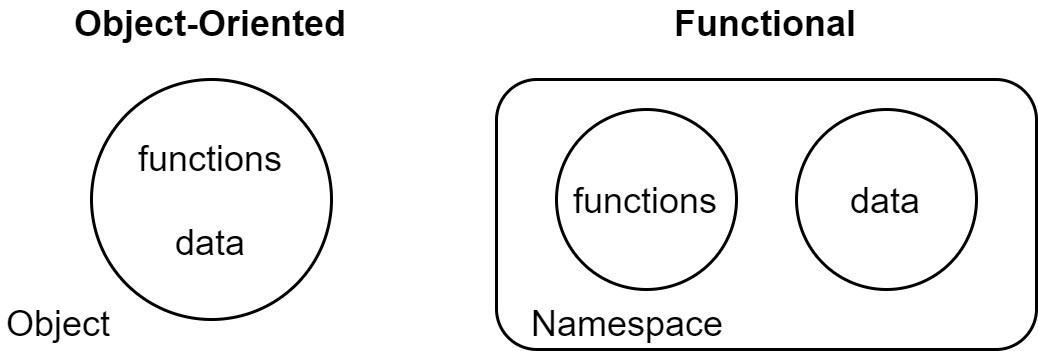
\includegraphics{lesson19/functions-and-data.png}
\end{figure}


\subsection{Example: Modeling a Domain}

Say that we have been tasked with creating an analytics app. Before we
get started, we want to model the type of objects that we will be
working with. If we were using a statically typed language, we would
probably start by writing type definitions. Even if we were working in
JavaScript, we would likely define ``classes''\index{object-oriented programming} for the objects that we
will be working with. As we define these objects, we would have to think
about both the data that they contain and the operations that they
support. For example, if we have a \texttt{User} and a
\texttt{ClickEvent}, we might need the operation,
\texttt{User.prototype.clickEvent()}.

\begin{figure}[H]
\caption{Analytics domain: users and their actions}
\centering
\includegraphics{lesson19/analytics-domain.png}
\end{figure}

With ClojureScript, we will consider data and functions separately. This
approach ends up being flexible, as we will see that most of the
operations that we want to perform on the data are simple and re-usable.
In fact, it is common to find that the exact operation that you need is
already part of the standard library. Ultimately, the combination of the
concision of code and the richness of the standard library means that we
write fewer lines of code than we would in JavaScript, which leads to
more robust and maintainable applications.\index{scaling issues}


\section{Domain Modeling with Maps and Vectors}

We are now quite familiar with maps and vectors as well as some of the
collection and sequence operations that can be used on them. Now we can
put them in practice in a real domain: an analytics dashboard. The main
concepts that we need to model are \emph{user}, \emph{session},
\emph{page-view}, and \emph{event}, and the relationships between these
models are as follows:

\begin{itemize}
\tightlist
\item
  A user has one or more sessions
\item
  A session has one or more page-views and may belong to a user or be
  anonymous
\item
  A page-view has zero or more events
\end{itemize}

We now know enough to create some sample data. Let's start at the
``bottom'' with the simplest models and work our way up to the
higher-level models. Since an \emph{event} does not depend on any other
model, it is a good place to start.


\subsection{Modeling Events}

An event is some action that the user performs while interacting with a
web page. It could be a \emph{click}, \emph{scroll}, \emph{field entry},
etc. Different events may have different properties associated with
them, but they all have at least a type and a timestamp.

\begin{lstlisting}[language=Clojure, caption={Modeling an event}]
(def my-event {:type :click                                %\circled{1}%
               :timestamp 1464362801602
               :location [1015 433]                        %\circled{2}%
               :target "#some-elem"})
\end{lstlisting}

\begin{enumerate}[label=\protect\circled{\arabic*}]
\tightlist
\item
  Every event will have \texttt{:type} and \texttt{:timestamp} entries
\item
  The remaining entries will be specific to the event type
\end{enumerate}

When we think of data types like \emph{event} in ClojureScript, we
usually create at least a mental schema of the data type. There are
libraries that we can use to enforce a schema on our data, most notably
\index{clojure.spec}clojure.spec\footnote{https://clojure.org/about/spec}, but for now we will
just enforce the ``shape'' of our data structures by convention. That
is, we will ensure that whenever we create an event, we create it with a
timestamp and a type. In fact, \index{constructor function}it is a common practice to define one or
more functions for constructing the new data types that we create. Here
is an example for how we might do this with \emph{events}:

\begin{lstlisting}[language=Clojure, caption={Using a constructor function}]
cljs.user=> (defn event [type]
              {:type type
               :timestamp (.now js/Date)})
#'cljs.user/event

cljs.user=> (event :click)
{:type :click, :timestamp 1464610050488}}]

\end{lstlisting}

This function simply abstracts the process of creating a new object that
follows the convention that we have established for events. We should
also create a constructor function for click events specifically:

\begin{lstlisting}[language=Clojure]
cljs.user=> (defn click [location target]
              (merge (event :click)
                     {:location location, :target target}))
#'cljs.user/click

cljs.user=> (click [644 831] "#somewhere")
{:type :click,
 :timestamp 1464610282324,
 :location [644 831],
 :target "#somewhere"}
\end{lstlisting}

\index{collection operations!merge@\texttt{merge}}The only thing about this code that might be unfamiliar is the use of
the \texttt{merge} function. It takes at least two maps and returns a
new map that is the result of adding all properties from each subsequent
map to the first one. You can think of it as \texttt{conj}-ing every
entry from the second map onto the first.


\subsection{Quick Review: Merge}

\begin{itemize}
\tightlist
\item
  In the REPL, define 2 maps and merge them together
\item
  Define 3 maps and merge them together,
  e.g.~\texttt{(merge\ map-1\ map-2\ map-3)}
\item
  Does \texttt{merge} mutate (change) any of the maps that we pass in?
\item
  What is the result of the following expression?
\end{itemize}

\begin{lstlisting}[language=Clojure]
(let [orig {:name "Cookie Monster" :food "Cookies!!"}
      overwrite {:profession "puppet" :food "Lasagne"}]
  (merge orig overwrite))
\end{lstlisting}


\subsection{You Try It}

\begin{itemize}
\tightlist
\item
We are representing coordinates on a page with a 2-element vector
containing, \texttt{{[}x-position,\ y-position{]}}. Define a function,
\texttt{location}, that will create a location given two numbers, such
that the following expressions will yield the same result:

\begin{lstlisting}[language=Clojure]
;; Expression 1 - Define location inline
(click [644 831] ".link")

;; Expression 2 - Construct location with a function
(click (location 644 831) ".link")
\end{lstlisting}
\end{itemize}

\begin{notice}[title={A Word on Constructors}]
We have been talking about the concept of \emph{constructors} in
ClojureScript. Unlike JavaScript, constructors in ClojureScript are just
plain functions that return data. There is no special treatment of
constructor functions in the language - they are merely a convenience
for us developers to easily create new data while consolidating the
creation code in one place.
\end{notice}


\subsection{Modeling page-views}

With events done, we can now model page-views. We will go ahead and
define a constructor for page-views:

\begin{lstlisting}[language=Clojure, caption={Modeling a page-view}]
cljs.user=> (defn page-view
              ([url] (page-view url (.now js/Date) []))     %\circled{1}%
              ([url loaded] (page-view url loaded []))
              ([url loaded events]
                {:url url
                 :loaded loaded
                 :events events}))

cljs.user=> (page-view "some.example.com/url")              %\circled{2}%
{:url "some.example.com/url",
 :loaded 1464612010514,
 :events []}

cljs.user=> (page-view "http://www.example.com"             %\circled{3}%
                      1464611888074
                      [(click [100 200] ".logo")])
{:url "http://www.example.com",
 :loaded 1464611888074,
 :events [{:type :click,
           :timestamp 1464611951519,
           :location [100 200],
           :target ".logo"}]}
\end{lstlisting}

\begin{enumerate}[label=\protect\circled{\arabic*}]
\tightlist
\item
  Define \texttt{page-view} with 3 arities
\item
  \texttt{page-view} can be called with just a URL
\item
  \ldots{}or with a URL, loaded timestamp, and vector of events
\end{enumerate}

Just as we did with events, we created a constructor to manage the
details of assembling a map that fits our definition of what a
\emph{page-view} is. One different aspect of this code is that we are
using a multiple-arity function as the constructor and providing default
values for the \texttt{loaded} and \texttt{events} values when they are
not supplied. \index{arguments!default values}This is a common pattern in ClojureScript for dealing with
default values for arguments.


\subsection{Modeling Sessions}

Moving up the hierarchy of our data model, we now come to the
\emph{Session}. Remember that a session represents one or more
consecutive page-views from the same user. If a user leaves the site and
comes back later, we would create a new session. So the session needs to
have a collection of page-views as well as identifying information about
the user's browser, location, etc.

\begin{lstlisting}[language=Clojure, caption={Modeling a session}]
  cljs.user=> (defn session
  ([start is-active? ip user-agent] (session start is-active? ip user-agent []))
  ([start is-active? ip user-agent page-views]
    {:start start
     :is-active? is-active?
     :ip ip
     :user-agent user-agent
     :page-views page-views}))

cljs.user=> (session 1464613203797 true "192.168.10.4" "Some UA")
{:start 1464613203797, :is-active? true, :ip "192.168.10.4", :user-agent "Some UA", :page-views []}
\end{lstlisting}

There is nothing new here. We are simply enriching our domain with more
types that we will be able to use in an analytics application. The only
piece that remains is the \emph{User}.


\subsection{You Try It}

Now that we have walked through the definition of \emph{events},
\emph{page-views}, and \emph{sessions}, you have all of the tools that
you need to define a data type for users.

\begin{itemize}
\tightlist
\item
  Define the ``shape'' of a user. It should include at least the
  following: \texttt{:id}, \texttt{:name}, \texttt{:sessions}.
\item
  Create a constructor function that can create a user with or without a
  collection of sessions
\item
  For extra credit, create another function called
  \texttt{anonymous-user} that creates a user that has no id or name
\end{itemize}

We now have a fairly complete domain defined for our analytics
application. Next, we'll explore how we can interact with it using
primarily functions from ClojureScript's standard library. Below is a
sample of what some complete data from our domain looks like at this
point. It will be helpful to reference this data as we move on.

\begin{lstlisting}[language=Clojure, caption={Sample data for an analytics domain}]
;; User
{:id 123
 :name "John Anon"
 :sessions [

   ;; Session
   {:start 1464379781618
    :is-active? true
    :ip 127.0.0.1
    :user-agent "some-user-agent"
    :page-views [

      ;; Pageview
      {:url "some-url"
       :loaded 1464379918936
       :events [

         ;; Event
         {:type :scroll
          :location [403 812]
          :distance 312
          :timestamp 1464380102036}

         ;; Event
         {:type :click
          :location [644 112]
          :target "a.link.about"
          :timestamp 1464380117760}]}]}]}
\end{lstlisting}


\section{Working With Associative Data}

Most of our analytics data is in the form of maps, which are simple
key-value associations. As we have just seen, there is quite a lot of
data that can be modeled using only maps, so it stands to reason that
ClojureScript would provide good tools for operating on them. This is
indeed the case. We will look at several functions that we will keep
coming back to when we work with maps: \texttt{assoc}, \texttt{dissoc},
and \texttt{select-keys}. There are more function in the standard
library that can be used on maps, but these are the most commonly used
and deserve some explanation.
The Clojure Cheatsheet\footnote{http://clojure.org/api/cheatsheet} is an
excellent reference for the functions that we will not be able to cover.

\subsection{More or Less: Adding and Removing Elements}

ClojureScript has a very helpful pair of functions for adding and
removing map entries: \texttt{assoc} and \texttt{dissoc}. Unlike setting
and deleting JavaScript object properties, \texttt{assoc} and
\texttt{dissoc} do not touch the maps that we supply. Instead, they
return new maps. By now, we should be familiar with the idea of working
with immutable data, but it still takes some getting used to.


\subsubsection{Adding Values With \texttt{assoc}}

\index{collection operations!assoc@\texttt{assoc}}Let's consider the \emph{session} model that we just created. It has
identifying information about user's visit to our website. Our new
requirement is to add a \emph{duration} to every session once the user
has logged out or left the site. In this case, we just need to add a new
entry to the session map - let's call it \texttt{:duration}.

\begin{figure}[H]
\caption{Associating data into a map}
\centering
\includegraphics{lesson19/assoc.png}
\end{figure}

This is exactly the case that the \texttt{assoc} function solves:
associating some key with a value inside a map. \texttt{assoc} takes a
map and a key and value to associate into the map. It can also accept
any additional number of keys and values as arguments, and it will
associate all of the keys and values in the map.

\begin{lstlisting}[language=Clojure, caption={Adding entries to a map}]
cljs.user=> (def trail {:name "Bear Creek Trail"
                        :distance 7.5})
#'cljs.user/trail

cljs.user=> (assoc trail :difficulty :moderate)            %\circled{1}%
{:name "Bear Creek Trail",
 :distance 7.5,
 :difficulty :moderate}

cljs.user=> (assoc trail                                   %\circled{2}%
                   :difficulty :moderate
                   :location "Colorado"
                   :max-elevation 12800)
{:name "Bear Creek Trail",
 :distance 7.5,
 :difficulty :moderate,
 :location "Colorado",
 :max-elevation 12800}
\end{lstlisting}

\begin{enumerate}[label=\protect\circled{\arabic*}]
\tightlist
\item
  Adding a single entry
\item
  Adding multiple entries
\end{enumerate}

With that, we can write a function that, given an end timestamp, will
add a \texttt{:duration} entry with the number of seconds in the
session:

\begin{lstlisting}[language=Clojure]
cljs.user=> (defn with-duration [session end-time]
              (let [duration-in-ms (- end-time (:start session))
                    duration-in-s (.floor Math (/ duration-in-ms 1000))]
                (assoc session :duration duration-in-s)))

cljs.user=> (def my-session
              (session (.now js/Date) true "127.0.0.1" "Some UA"))
#'cljs.user/my-session

;; Wait a few seconds

cljs.user=> (with-duration my-session (.now js/Date))
{:start 1464641029299,
 :is-active? true,
 :ip "127.0.0.1",
 :user-agent "Some UA",
 :page-views [],
 :duration 14}
\end{lstlisting}

\subsubsection{Mini Review: \texttt{assoc}}

\begin{itemize}
\tightlist
\item
  Is there a difference between \texttt{(assoc\ some-map\ key\ val)} and
  \texttt{(conj\ some-map\ {[}key\ val{]})}?
\item
  Does assoc mutate (change) the map that is passed in?
\end{itemize}


\subsection{Removing Values With \texttt{dissoc}}

\index{collection operations!dissoc@\texttt{dissoc}}Now imagine that we have added a setting where users can request that we
not track their IP or user agent, so we will need to remove this data
from the map before we send it off to the server. This is exactly the
functionality that \texttt{dissoc} gives us: it takes a map and any
number of keys to remove from the map, and it returns a new map without
the keys we specified. Let's create a function, \texttt{untrack}, that
returns a session without these entries:

\begin{lstlisting}[language=Clojure]
cljs.user=> (defn untrack [session]
              (dissoc session :ip :user-agent))
#'cljs.user/untrack

cljs.user=> (untrack my-session)
{:start 1464641029299, :is-active? true, :page-views []}
\end{lstlisting}

\subsubsection{Mini Review: \texttt{dissoc}}

\begin{itemize}
\tightlist
\item
  Use \texttt{dissoc} to remove the \texttt{:region} key from this map:
  \texttt{\{:landmark\ "Uncompahgre",\ :region\ "San\ Juan\ Mountains"\}}
\item
  What happens when the map does not contain one or more of the keys
  that we pass to \texttt{dissoc},
  e.g.~\texttt{(dissoc\ \{:temp\ 212\}\ :color\ :material\ :mass)}?
\item
  Update the \texttt{with-duration} function that we created earlier to
  remove the \texttt{:is-active?} key from the session.
\end{itemize}


\subsection{Refining a Selection With \texttt{select-keys}}

\index{collection operations!select-keys@\texttt{select-keys}}Another handy function to have in our toolbox when working with maps is
\texttt{select-keys}. It takes a map and a collection of keys to retain,
and it returns a new map with only the keys that were passed in. If we
had some portion of the application that was only interested in when a
session started, whether it was active, and its page-views, we could use
\texttt{select-keys} to narrow down the data to only what we are
interested in:

\begin{lstlisting}[language=Clojure]
cljs.user=> (select-keys my-session [:start :is-active? :page-views])
{:start 1464641029299,
 :is-active? true,
 :page-views []}
\end{lstlisting}


\subsection{You Try It}

It is intuitive that ClojureScript considers maps to be associative.
Interestingly, vectors are also associative collections that map an
integer index to the element at that index:

\begin{lstlisting}[language=Clojure]
cljs.user=> (associative? [])
true
\end{lstlisting}

\begin{itemize}
\tightlist
\item
  Define a vector with several elements at the REPL
\item
  Use \texttt{get} to retrieve the element at a specific index
\item
  Use \texttt{assoc} to update the element at a specific index
\item
  Try using the \texttt{merge} and \texttt{dissoc}, functions on the
  vector. Do the results surprise you?
\end{itemize}


\section{Working With Nested Data}

\index{nested data}In any but the simplest of programs, we will need to work with nested
data at some point. The analytics application that we are considering in
this chapter is a good example, since we have events nested inside
page-views, which are in turn nested inside sessions, which themselves
are nested inside users. Using only the functions we have seen so far
would be intractable at best. We will now turn our attention to several
functions that allow us to work with nested data.


\subsection{Drilling Down With \texttt{get-in}}

\index{collection operations!get-in@\texttt{get-in}}We have seen the \texttt{get} function a number of times for accessing a
specific element in a map or a vector. It has a cousin, \texttt{get-in},
that is used for setting values that are nested deeper inside a data
structure. Instead of supplying a single key for the value to get out,
we supply a sequence of keys that will be looked up in turn. We can
think of this sequence as a \emph{path} to the data that we are
interested in. It is like a road map for the computer to follow to
locate the data to retrieve. For instance, to get the first page-view of
the first session of some user, we could use something like the
following:

\begin{lstlisting}[language=Clojure]
(get-in user [:sessions 0 :page-views 0])
\end{lstlisting}

\emph{Getting Nested Data}

This will first look up the \texttt{:sessions} key on the \texttt{user}
that we passed in. Next, it will get the first session (at index 0),
then it will get the \texttt{:page-views} key on this session. Finally,
it will get the first of the page-views. Notice that the get-in is really
just a convenience for repeated calls to \texttt{get}:

\begin{lstlisting}[language=Clojure]
(get
  (get
    (get
      (get user :sessions)                                 %\circled{1}%
     0)                                                    %\circled{2}%
   :page-views)                                            %\circled{3}%
  0)                                                       %\circled{4}%
\end{lstlisting}

\begin{enumerate}[label=\protect\circled{\arabic*}]
\tightlist
\item
  Get the user's sessions
\item
  Get the first
\item
  Get the page-views
\item
  Get the first
\end{enumerate}

This concept of a \emph{path} is used commonly in ClojureScript to
describe how to ``get to'' some specific piece of data. An analogy in
the JavaScript world would be chained property access on some specific
object:

\begin{lstlisting}[language=JavaScript, caption={Getting nested data with JavaScript}]
user.sessions[0].pageViews[0];
\end{lstlisting}

At first glance, the JavaScript version looks at least as clear as the
ClojureScript version - in fact, perhaps a bit clearer. However, one key
feature of get-in is that if at any point in the path the next property
does not exist, the evaluation will stop, and the whole thing will
evaluate to \texttt{nil}. A more accurate JavaScript translation would
be the following\footnote{JavaScript's new optional chaining feature would simplify this expression as  \texttt{user?.sessions?{[}0{]}?.pageViews?{[}0{]}}}:

\begin{lstlisting}[language=JavaScript]
user &&                                                    %\circled{1}%
    user.sessions &&
    user.sessions[0] &&
    user.sessions[0].pageViews &&
    user.sessions[0].pageViews[0];                         %\circled{2}%
\end{lstlisting}

\begin{enumerate}[label=\protect\circled{\arabic*}]
\tightlist
\item
  Check every intermediate step that may be undefined
\item
  Only get the nested data if every step in the path to it is defined
\end{enumerate}


\subsubsection{Mini Review: \texttt{get-in}}

\begin{itemize}
\tightlist
\item
  Fill in the blank to make this expression true
\end{itemize}

\begin{lstlisting}[language=Clojure]
(= "second"
   (get-in {:tag "ul"
            :children [{:tag "li"
                        :id "first"}
                       {:tag "li"
                        :id "second"}]}
           ...)
\end{lstlisting}

\begin{itemize}
\tightlist
\item
  What does the following expression evaluate to?
\end{itemize}

\begin{lstlisting}[language=Clojure]
(get-in {} [:does :not :exist])
\end{lstlisting}

\subsection{Setting With \texttt{assoc-in}}

\index{collection operations!assoc-in@\texttt{assoc-in}}Just as \texttt{get-in} is a variation of \texttt{get} that allows for
nested data access, \texttt{assoc-in} is a variation of \texttt{assoc}
that allows for the setting of nested data. Calling \texttt{assoc-in} is
very similar to calling \texttt{assoc} - the difference is that instead
of supplying a simple key, we pass in a path to the data that we want to
set.

\begin{lstlisting}[language=Clojure]
(assoc-in user
          [:sessions 0 :page-views]                        %\circled{1}%
          [(page-view "www.learn-cljs.com" 123456 [])])    %\circled{2}%
\end{lstlisting}

\begin{enumerate}[label=\protect\circled{\arabic*}]
\tightlist
\item
  Path to the data to update
\item
  Value to associate
\end{enumerate}


\subsubsection{Mini Review: \texttt{assoc-in}}

\begin{itemize}
\tightlist
\item
  What is the result of the following:
\end{itemize}

\begin{lstlisting}[language=Clojure]
(assoc-in {:tag "ul"
           :children [{:tag "li"
                       :id "first"}
                      {:tag "li"
                       :id "second"}]}
          [:children 1 :class]
          "last-item")`
\end{lstlisting}

\begin{itemize}
\tightlist
\item
  What is the result of the following:
\end{itemize}

\begin{lstlisting}[language=Clojure]
(assoc-in {} [:foo :bar :baz] "quux")
\end{lstlisting}


\subsection{Updating With \texttt{update-in}}

\index{collection operations!update-in@\texttt{update-in}}Now that we have seen how \texttt{get-in} and \texttt{assoc-in} work, it
is time to complete our trio of functions for working with nested data
with \texttt{update-in}. Like \texttt{assoc-in}, it takes a data
structure and a path, but instead of taking a simple value to put into
the data structure, it takes a function to apply to the existing item
that it finds at the specified path. The entry at this path is then
replaced with whatever the function returns. Let's consider a simple
example:

\begin{lstlisting}[language=Clojure]
cljs.user=> (update-in {:num 1} [:num] inc)
{:num 2}
\end{lstlisting}

In this case, we specified that we wanted to operate on the element
located at the path \texttt{{[}:num{]}} and increment it. This yielded a
new map in which the \texttt{:num} key is the increment of the
\texttt{:num} key in the original map. In this simple example, we worked
with flat data, but the principle is the same for nested data. Going
back to the analytics example, let's say that we wanted to add 10 pixels to
the x-coordinate of a click event. We could easily accomplish this with
a single \texttt{update-in}:

\begin{lstlisting}[language=Clojure]
(defn add-to-click-location [click-event]
  (update-in [:location 0] #(+ 10 %\%%)))
\end{lstlisting}

When we start building single-page apps with Reagent, we will constantly
be making use of \texttt{update-in}, so it is important to make sure
that we are comfortable with how to use it.


\subsubsection{Mini Review: \texttt{update-in}}

\begin{itemize}
\tightlist
\item
  What is the result of
  \texttt{(update-in\ \{\}\ {[}:foo\ :bar{]}\ inc)}?
\item
  Does update-in work with both maps and vectors? Why or why not?
\end{itemize}


\section{Summary}

We covered a lot of ground in this chapter, and we are now able to do
quite a bit of data manipulation, including:

\begin{itemize}
\tightlist
\item
  Combining maps with \texttt{merge}
\item
  Adding and removing single properties with \texttt{assoc} and
  \texttt{dissoc}
\item
  Working with deeply nested data using \texttt{get-in},
  \texttt{assoc-in}, and \texttt{update-in}
\end{itemize}

Between the sequence operations that we covered in the last lesson and
the additional operations that we just learned, we can write quite
intricate, data-driven programs. Next up, we'll put together all that we
have learned about collections and sequences to build a contact list
application that keeps its data in \texttt{localStorage}.

\chapter{Capstone 3 - Contact Book}

Over the past few lessons, we have learned the core tools for working
with data in ClojureScript. First, we learned about the basic collection
types - lists, vectors, maps, and sets - as well as the most common
functions for working with these collections. Then we took a closer look
at the important \emph{sequence abstraction} that allows us to operate
on all sorts of sequential data using a uniform interface. Next, we
discovered the \texttt{reduce} function and the many cases in which it
can be used to summarize a sequence of data. Last, we walked through the
process of modeling a real- world analytics domain. With this knowledge
in our possession, we are ready to build another capstone project. This
time, we will take the example of a contact book that we mentioned back
in Lesson 16, and we will build a complete implementation,
\emph{ClojureScript Contacts}.

\begin{center}\rule{0.5\linewidth}{0.5pt}\end{center}

\textbf{In this lesson:}

\begin{itemize}
\tightlist
\item
  Create a complete ClojureScript application without any frameworks
\item
  Build HTML out of plain ClojureScript data structures
\end{itemize}

\begin{center}\rule{0.5\linewidth}{0.5pt}\end{center}

\begin{figure}[H]
\centering
\includegraphics[width=12cm]{lesson20/contacts-screenshot.png}
\end{figure}


While we will not be printing the code for this capstone in its entirety, the completed project code may be found at the book's GitHub project\footnote{https://github.com/kendru/learn-cljs/tree/master/code/lesson-20/contacts}. As we have done previously, we will create a new Figwheel project:

\begin{verbatim}
$ clj -X:new :template figwheel-main :name learn-cljs/contacts :args '["+deps"]'
$ cd contacts
$ clj -A:fig:build
\end{verbatim}

\section{Data Modeling}

In this lesson, we will use the techniques and patterns from the
previous chapter to model the data for our contact book. The goal will
be to practice what we have learned rather than to introduce much new
material. We will primarily model our data using maps and vectors, and
we will implement the constructor function pattern for creating new
contacts. We will also implement the operations that the UI will need to
update the contact list using simple functions to transform our data.
With that, let's dig in to the data model!


\subsection{Constructing Entities}

Since a contact book represents an ordered list of contacts, we will
need a data structure to represent that ordered list, and as we have
already seen, a vector fits the bill nicely. We can define an empty
contact list as an empty vector - no constructor function necessary:

\begin{lstlisting}[language=Clojure]
(def contact-list [])
\end{lstlisting}

Since an empty vector is not terribly interesting, let's turn our
attention to the contacts that it will hold. Each contact will need a
first name, last name, email address, and a physical address, including
city, state, and country. This can easily be accommodated with a nested
map, such as the following:

\begin{lstlisting}[language=Clojure]
{:first-name "Phillip"
 :last-name "Jordan"
 :email "phil.j@hotmail.com"
 :address {:street "523 Sunny Hills Cir."
           :city "Springfield"
           :state "MI"
           :postal "11111"
           :country "USA"}}
\end{lstlisting}

In order to construct a new contact, we will use a variation on the
constructor pattern introduced in the last lesson. Instead of passing in
each field individually, we will pass in a map that we expect to contain
zero or more of the fields that make up a contact. You will recall from
the last lesson that the \texttt{select-keys} function takes a map and a
collection of keys that should be selected, and it returns a new map
with only the selected keys copied. We can use this function to sanitize
the input, ensuring that our contact contains only valid keys.

\begin{lstlisting}[language=Clojure]
(defn make-contact [contact]
  (select-keys contact [:first-name :last-name :email :postal :address]))
\end{lstlisting}

Since the address itself is a map, let's factor out creation of an
address to another function. We can then update the
\texttt{make-contact} function to use this address constructor:

\begin{lstlisting}[language=Clojure]
(defn make-address [address]
  (select-keys address [:street :city :state :country]))

(defn make-contact [contact]
  (let [clean-contact (select-keys contact [:first-name :last-name :email])]
    (if-let [address (:address contact)]
      (assoc clean-contact :address (make-address address))
      clean-contact)))
\end{lstlisting}

This new version of \texttt{make-contact} introduces one expression that
we have not seen before: \texttt{if-let}. This macro works just like
\texttt{if} except that it binds a name to the value being tested (just
like \texttt{let} does). Unlike \texttt{let}, only a single binding may
be provides. At compile time, this code will expand to something like
the following\footnote{The actual implementation of the \texttt{if-let}
  macro is slightly more complex, but the effect is the same.}:

\begin{lstlisting}[language=Clojure, caption={\texttt{if-let} transformation}]
(if (:address contact)
  (let [address (:address contact)]
    (assoc clean-contact :address (make-address address)))
  clean-contact)
\end{lstlisting}

We will soon make use of a similar macro, \texttt{when-let}. Like \texttt{if-let}, it allows a binding to be provided, and like \texttt{when}, it only handles the case when the bound value is non-nil.

\index{threading macros}However, we can make the \texttt{make-contact} function a bit more
concise and easier to read using one of ClojureScript's \emph{threading
macros}, \texttt{-\textgreater{}} (pronounced ``thread first''). This
macro allows us to take what would otherwise be a deeply nested
expression and write it more sequentially. It takes a value and any
number of function calls and injects the value as the first argument to
each of these function calls. Seeing this transformation in action
should make its functionality more intuitive:

\begin{lstlisting}[language=Clojure, caption={Thread-first transformation}]
(-> val                                                    %\circled{1}%
    (fn-1 :foo)                                            %\circled{2}%
    (fn-2 :bar :baz)                                       %\circled{3}%
    (fn-3))

(fn-3                                                      %\circled{4}%
  (fn-2
    (fn-1 val :foo)
    :bar :baz))
\end{lstlisting}

\begin{enumerate}[label=\protect\circled{\arabic*}]
\tightlist
\item
  Start with \texttt{val} as the value to thread through the following
  expressions
\item
  \texttt{fn-1} will be evaluated with the arguments, \texttt{val} and
  \texttt{:foo}
\item
  The result of the evaluation of \texttt{fn-1} will be threaded as the
  first argument to \texttt{fn-2}
\item
  The macro will rewrite into a nested expression that evaluates
  \texttt{fn-1} then \texttt{fn-2}, then \texttt{fn-3}
\end{enumerate}

This macro is extremely common in ClojureScript code because of how it
enhances the readability of our code. We can write code that looks
sequential but is evaluated ``inside-out''. There are several additional
threading macros in ClojureScript that we will not go into now, but we
will explain their usage as we run into them.

\begin{figure}[H]
\caption{Thread first macro}
\centering
\includegraphics{lesson20/thread-first.png}
\end{figure}

With this macro, we can make our \texttt{make-contact} function even
clearer:

\begin{lstlisting}[language=Clojure]
(defn maybe-set-address [contact]                          %\circled{1}%
  (if (:address contact)
    (update contact :address make-address)
    contact))

(defn make-contact [contact]
  (-> contact                                              %\circled{2}%
      (select-keys [:first-name :last-name :email])
      (maybe-set-address)))
\end{lstlisting}

\begin{enumerate}[label=\protect\circled{\arabic*}]
\tightlist
\item
  Refactor the code that conditionally constructs an address
\item
  Rewrite \texttt{make-contact} using the \texttt{-\textgreater{}} macro
\end{enumerate}


\subsection{Quick Review}

\begin{itemize}
\tightlist
\item
  Does \texttt{if-let} allow multiple bindings? For example, what would
  this code do?
\end{itemize}

\begin{lstlisting}[language=Clojure]
(if-let [contact (find-by-id 123)
         address (:address contact)]
  (println "Address:" (format-address address)))
\end{lstlisting}

\begin{itemize}
\tightlist
\item
  How would the \texttt{-\textgreater{}} macro rewrite the following
  expression?
\end{itemize}

\begin{lstlisting}[language=Clojure]
(let [input {:password "s3cr3t"}]
  (-> input
      (assoc :password-digest (-> input :password digest))
      (dissoc :password)))
\end{lstlisting}

\subsection{Defining State Transitions}

In order for our UI to do anything other than display a static list of
contacts that we define in code, we need to enable some interactions in
the UI. Again, we are building our low-level domain logic before any UI
code so that we can take advantage of the bottom-up programming style
that ClojureScript encourages - composing small, granular functions into
larger and more useful structures.

First, we want the user to be able to add a new contact to the contact
list. We can assume that we will receive some sort of form data as
input, which we can pass to our \texttt{make-contact} constructor,
adding the resulting contact to our list. We will need to pass in the
contact list and input data as arguments and produce a new contact list.

\begin{lstlisting}[language=Clojure]
(defn add-contact [contact-list input]
  (conj contact-list
        (make-contact input)))
\end{lstlisting}

We can paste these function definitions into the REPL and then test them
to make sure that they function as expected:

\begin{lstlisting}[language=Clojure]
cljs.user=> (-> contact-list                               %\circled{1}%
                (add-contact {:email "me@example.com"
                              :first-name "Me"
                              :address {:state "RI"}})
                (add-contact {:email "you@example.com"
                              :first-name "You"}))
[{:first-name "Me", :email "me@example.com"}
 {:first-name "You", :email "you@example.com"}]
\end{lstlisting}

\emph{Testing with the REPL}

\begin{enumerate}[label=\protect\circled{\arabic*}]
\tightlist
\item
  Once again, the \texttt{-\textgreater{}} macro makes our code easier
  to read and write
\end{enumerate}

Next, we will need a way to remove a contact from the list. Since we are
using a vector to hold our contacts, we can simply remove an element at
a specific index:

\begin{lstlisting}[language=Clojure, caption={Removing a contact}]
(defn remove-contact [contact-list idx]
  (vec                                                     %\circled{1}%
    (concat                                                %\circled{2}%
      (subvec contact-list 0 idx)                          %\circled{3}%
      (subvec contact-list (inc idx)))))
\end{lstlisting}

\begin{enumerate}[label=\protect\circled{\arabic*}]
\tightlist
\item
  \texttt{vec} converts a sequence into a vector
\item
  \texttt{concat} returns a \texttt{seq} that contains all elements in
  the sequences passed to it in order
\item
  \texttt{subvec} returns a portion of the vector that it is given
\end{enumerate}

Since there are a couple of new functions here that we have not seen
yet, let's quickly look at what they do. Starting from the ``inside'' of
this function, we have \texttt{subvec}. This function provides an
efficient way to obtain a slice of some vector. It comes in a 2-arity
and a 3-arity form: \texttt{(subvec\ v\ start)} and
\texttt{(subvec\ v\ start\ end)}. This function work similarly to
JavaScript's \texttt{Array.prototype.slice()} function. It returns a new
vector that starts at the \texttt{start} index of the original vector
and contains all elements up to but not including the \texttt{end}
index. If no \texttt{end} is provided, it will contain everything from
\texttt{start} to the end of the original vector.

\index{sequence operations!concat@\texttt{concat}}Next, we have \texttt{concat}. This function takes a number of sequences
and creates a new lazy\footnote{Lazy evaluation was covered in
Lesson 11.} \texttt{seq} that is the concatenation of all of the elements of
its arguments. Because the result is a \texttt{seq}, we use the
\texttt{vec} function to coerce the result back into a vector. Since
much of ClojureScript's standard library operates on the sequence
abstraction, we will find that we often need to convert the result back
into a more specific type of collection.

Finally, when we update a contact, we want to replace the previous version. This can be done by using \texttt{assoc} to put the updated contact in the same index of \texttt{contact-list} that was occupied by the old version:

\begin{lstlisting}[language=Clojure]
(defn replace-contact [contact-list idx input]
  (assoc contact-list idx (make-contact input)))
\end{lstlisting}

\subsection{Quick Review}

\begin{itemize}
\tightlist
\item
  We mentioned that \texttt{vec} converts a sequence into a vector.
  Given what we learned about the sequence abstraction, what will happen
  if you pass \texttt{vec} a map? What about a set?
\end{itemize}


\section{Creating the UI}

Now that we have defined all of the functions that we need to work with
our data model, let's turn our attention to creating the application UI.
In Section 5, we will learn how to create high-performance UIs using the
Reagent framework, but for now, we will take naive approach of
re-rendering the entire application whenever anything changes. Our
application will have two main sections - a list of contacts that
displays summary details about each contact and a larger pane for
viewing/editing contact details.

We will use the \index{hiccup}hiccups\footnote{https://github.com/teropa/hiccups}
library to transform plain ClojureScript data structures into an HTML
string. This allows us to represent the interface of our application as
a ClojureScript data structure and have a very simple interface to the
actual DOM of the page. In order to use this library, we need to add it
to our dependencies in \texttt{deps.edn}:

\begin{lstlisting}[language=Clojure, caption={deps.edn}]
:deps {;; ...Other dependencies
       hiccups/hiccups {:mvn/version "0.3.0"}}
\end{lstlisting}

Then, we need to import this library into our \texttt{core} namespace.
Note that since we are using a macro from this library, the syntax is a
little different:

\begin{lstlisting}[language=Clojure, caption={learn\_cljs/contacts.cljs}]
(ns learn-cljs.contacts
  (:require-macros [hiccups.core :as hiccups])
  (:require [hiccups.runtime]))
\end{lstlisting}

The translation between ClojureScript data structures and HTML is very
simple:

\begin{enumerate}
\def\labelenumi{\arabic{enumi}.}
\tightlist
\item
  HTML tags are represented by vectors whose first element is the tag
  name as a keyword
\item
  Attributes are represented by maps and should come immediately after
  the tag name. Omitting attributes is fine.
\item
  Any remaining elements in the vector are children of the outer element
\end{enumerate}

For example, the following code renders a div containing a single anchor
tag:

\begin{lstlisting}[language=Clojure, caption={Rendering with hiccups}]
(hiccups/html                                              %\circled{1}%
  [:div                                                    %\circled{2}%
    [:a {:href "https://www.google.com"                    %\circled{3}%
         :class "external-link"}
        "Google"]])                                        %\circled{4}%
;; <div><a class="external-link" href="https://www.google.com">Google</a></div>
\end{lstlisting}

\begin{enumerate}[label=\protect\circled{\arabic*}]
\tightlist
\item
  The \texttt{html} macro renders hiccups data to an HTML string
\item
  Create a \texttt{div}. We do not need to specify any attributes
\item
  Create an \texttt{a} element with an attributes map as a child of the
  outer \texttt{div}
\item
  The \texttt{a} only contains text
\end{enumerate}

With this knowledge, we can start defining components for our various UI
elements that produce a hiccups-compatible data structure. We can
compose these functions together to create a data structure that
represents the entire UI, and we'll pass this to another function that
renders the whole structure to the page.


\subsection{UI State}

Let's take a quick step back and think about the additional state that
we need for the UI. First, we need to have a flag indicating whether we
are in editing mode. In editing mode, a form with contact details will
be displayed in the right-hand pane. Also, we need to keep track of
which contact has been selected for editing - in the case of a new
contact that has not been saved yet, this property will be \texttt{nil}
or omitted. Naturally, we also need the contacts on the application
state. This leaves us with a pretty simple state model to support
everything that we want in our UI:

\begin{lstlisting}[language=Clojure]
(def initial-state
  {:contacts contact-list
   :selected nil
   :editing? false})
\end{lstlisting}

We will also define a \texttt{refresh!} function that is responsible for
rendering the entire application and attaching event handlers every time
our state changes. \index{event handler}We must re-attach event handlers because we are replacing the DOM tree that contains our app, and our handlers remain attached to the DOM nodes that are discarded.

\begin{lstlisting}[language=Clojure]
(defn attach-event-handlers! [state])                      %\circled{1}%

(defn set-app-html! [html-str]
  (set! (.-innerHTML app-container) html-str))

(defn render-app! [state]
  (set-app-html!
    (hiccups/html
      [:div])))                                            %\circled{2}%

(defn refresh! [state]                                     %\circled{3}%
  (render-app! state)
  (attach-event-handlers! state))

(refresh! initial-state)                                   %\circled{4}%
\end{lstlisting}

\begin{enumerate}[label=\protect\circled{\arabic*}]
\tightlist
\item
  All event handlers that we need to attach will be attached in this
  function
\item
  We will replace the empty div with our actual application HTML
\item
  \texttt{refresh!} will be called every time that we update the
  application state
\item
  We kick off the application with an initial \texttt{refresh!} to
  render the page from \texttt{initial-state}
\end{enumerate}


\subsection{Rendering Contacts}

Let's start with the component that displays the contact summary in the
list. We will be using the \index{Bulma CSS}Bulma CSS framework to help with styling\footnote{Bulma's styles can be found in \texttt{bulma.min.css} in the corresponding lesson of this book's GitHub repository.}, so
most of the markup that we are generating is for the purpose of styling
the page. Additionally, we will be using the \index{Microns icon font}Microns\footnote{https://www.s-ings.com/projects/microns-icon-font/} icon font, which uses \texttt{mu-ICON} class names. 

\begin{lstlisting}[language=Clojure, caption={Rendering a contact summary}]
(defn format-name [contact]                                %\circled{1}%
  (->> contact                                             %\circled{2}%
       ((juxt :first-name :last-name))                     %\circled{3}%
       (str/join " ")))

(defn delete-icon [idx]
  [:span {:class "delete-icon"
          :data-idx idx}
    [:span {:class "mu mu-delete"}]])

(defn render-contact-list-item [idx contact selected?]
  [:div {:class (str "card contact-summary" (when selected? " selected"))
         :data-idx idx}                                    %\circled{4}%
    [:div {:class "card-content"}
      [:div {:class "level"}
        [:div {:class "level-left"}
          [:div {:class "level-item"}
            (delete-icon idx)
            (format-name contact)]]
        [:div {:class "level-right"}
          [:span {:class "mu mu-right"}]]]]])
\end{lstlisting}

\begin{enumerate}[label=\protect\circled{\arabic*}]
\tightlist
\item
  Extract the logic for a contact's display name into another function
\item
  Use the \texttt{-\textgreater{}\textgreater{}} (thread last) macro to
  pass a value through as the last argument to each subsequent function
\item
  The \texttt{juxt} function extracts the first and last name from the
  contact. It is described below
\item
  \texttt{idx} is needed so that we will be able to get the correct
  contact in our event handlers
\end{enumerate}

\index{threading macros}Both of the things that we should note about this code occur in the
\texttt{format-name} function. First, we use the
\texttt{-\textgreater{}\textgreater{}} macro to thread a value through
several function calls. This works almost exactly like the
\texttt{-\textgreater{}} macro that we used earlier in this lesson with
the exception that it feeds threads the value as the \emph{last}
argument to each subsequent function.

\index{juxt@\texttt{juxt}}Second, the \texttt{juxt} function is a very interesting function that
deserves a bit of an explanation. \texttt{juxt} takes a variable number
of functions and returns a new function. This resulting function will
call each of the original functions passed to \texttt{juxt} in turn
using the arguments provided to it. The results are finally placed into
a vector in the same order as the functions that were passed to
\texttt{juxt}. For example, this code snippet will create a function
that will get 2-element vector containing the minimum and maximum values
from a collection:

\begin{lstlisting}[language=Clojure]
(def minmax
  (juxt #(reduce Math/min %\%%)
        #(reduce Math/max %\%%)))

(minmax [48 393 12 14 -2 207])
;; [-2 393]
\end{lstlisting}

The reason for the extra set of parentheses in the call to \texttt{juxt}
- \texttt{((juxt\ :first-name\ :last-name))} - is that we need to call
the function \emph{returned by} \texttt{juxt} rather than threading the
contact into the call to \texttt{juxt} itself. Since keywords are
functions that can look themselves up in maps, this expression will
effectively create a vector with the first name and last name of the
contact respectively.

\begin{lstlisting}[language=Clojure]
((juxt :first-name :last-name) {:first-name "Bob" :last-name "Jones"})
;; ["Bob" "Jones"]
\end{lstlisting}

\subsection{Adding Interactions}

Let's now think about the interactions that we want to enable on the
contact summary. When the row is clicked, we want to open up this
contact's details for view/editing. We will attach an event handler to
each list item that will set an \texttt{:editing?} flag on the app state
and will set \texttt{:selected} to the index of the contact that was
clicked (this is why we needed to pass \texttt{idx} into the rendering
function and set the \texttt{data-idx} attribute on the row).

\begin{lstlisting}[language=Clojure]
(defn on-open-contact [e state]
  (refresh!
    (let [idx (int (.. e -currentTarget -dataset -idx))]
      (assoc state :selected idx
                   :editing? true))))

(defn attach-event-handlers! [state]
  ;; ...
  (doseq [elem (array-seq (gdom/getElementsByClass "contact-summary"))]
    (gevents/listen elem "click"
      (fn [e] (on-open-contact e state)))))
\end{lstlisting}

We should be familiar with the use of \texttt{doseq} to eagerly iterate over a sequence,
but this is the first time we have seen \texttt{array-seq}. This function takes a JavaScript
array and transforms it into a ClojureScript seq that can be used with any sequence
operation - in this case, \texttt{doseq}.

Now that we can render a single contact list item, let's create the list
that will display each list item:

\begin{lstlisting}[language=Clojure]
(defn render-contact-list [state]
  (let [{:keys [:contacts :selected]} state]
    [:div {:class "contact-list column is-4 hero is-fullheight"}
      (map-indexed (fn [idx contact]
                     (render-contact-list-item idx contact (= idx selected)))
                   contacts)]))
\end{lstlisting}

This function is pretty straightforward: it renders a wrapper
\texttt{div} with each contact list item, then it delegates to the
\texttt{render-contact-list-item} function to render the summary for
each contact in turn. There is a new function that we have not yet met,
however: \texttt{map-indexed}. This function works just like
\texttt{map} except that it calls the mapping function with the index of
the element in the sequence as well as the element itself.

This pattern of building a UI by composing components is common in the
JavaScript world as well, but in most ClojureScript applications, the
method of composing UIs is function composition with pure functions that
produce plain data structures.

Finally, we will briefly cover rendering the contact details form and
adding/updating contacts without too much additional explanation. First,
let's look at the function that renders the entire app HTML:

\begin{lstlisting}[language=Clojure]
(defn render-app! [state]
  (set-app-html!
    (hiccups/html
      [:div {:class "app-main"}
        [:div {:class "navbar has-shadow"}
          [:div {:class "container"}
            [:div {:class "navbar-brand"}
              [:span {:class "navbar-item"}
                "ClojureScript Contacts"]]]]
        [:div {:class "columns"}
          (render-contact-list state)
          [:div {:class "contact-details column is-8"}
            (section-header (:editing? state))
            [:div {:class "hero is-fullheight"}
              (if (:editing? state)
                (render-contact-details (get-in state [:contacts (:selected state)] {}))
                [:p {:class "notice"} "No contact selected"])]]]])))
\end{lstlisting}

We have already seen the \texttt{render-contact-list} function, but we
still need to define \texttt{page-header}, which will display the
buttons for adding or saving a contact, and
\texttt{render-contact-details}, which will render the edit form. Let's
start with \texttt{render-contact-details}:

\begin{lstlisting}[language=Clojure, caption={Rendering contact details}]
(defn form-field                                           %\circled{1}%
  ([id value label] (form-field id value label "text"))
  ([id value label type]
   [:div {:class "field"}
     [:label {:class "label"} label]
     [:div {:class "control"}
       [:input {:id id
                :value value
                :type type
                :class "input"}]]]))

(defn render-contact-details [contact]
  (let [address (get contact :address {})]                 %\circled{2}%
    [:div {:id "contact-form" :class "contact-form"}
      (form-field "input-first-name" (:first-name contact) "First Name")
      (form-field "input-last-name" (:last-name contact) "Last Name")
      (form-field "input-email" (:email contact) "Email" "email")
      [:fieldset
        [:legend "Address"]
        (form-field "input-street" (:street address) "Street")
        (form-field "input-city" (:city address) "City")
        (form-field "input-state" (:state address) "State")
        (form-field "input-postal" (:postal address) "Postal Code")
        (form-field "input-country" (:country address) "Country")]]))
\end{lstlisting}

\begin{enumerate}[label=\protect\circled{\arabic*}]
\tightlist
\item
  Since we will be rendering multiple form fields, we will extract the
  code for a field into its own function
\item
  The address may or may not be present, so we provide an empty map as a
  default
\end{enumerate}

Now let's look at the code for processing the form and either adding or
updating a contact:

\begin{lstlisting}[language=Clojure]
(defn get-field-value [id]
  (let [value (.-value (gdom/getElement id))]
    (when (not (empty? value)) value)))

(defn get-contact-form-data []
  {:first-name (get-field-value "input-first-name")
   :last-name (get-field-value "input-last-name")
   :email (get-field-value "input-email")
   :address {:street (get-field-value "input-street")
             :city (get-field-value "input-city")
             :state (get-field-value "input-state")
             :postal (get-field-value "input-postal")
             :country (get-field-value "input-country")}})

(defn on-save-contact [state]
  (refresh!
    (let [contact (get-contact-form-data)
          idx (:selected state)
          state (dissoc state :selected :editing?)]        %\circled{1}%
      (if idx
        (update state :contacts                            %\circled{2}%
                replace-contact idx contact)
        (update state :contacts
                add-contact contact)))))
\end{lstlisting}

\begin{enumerate}[label=\protect\circled{\arabic*}]
\tightlist
\item
  \texttt{state} within the \texttt{let} will refer to this updated
  state
\item
  Use our domain functions to update the contact list within our app
  state
\end{enumerate}

\index{update@\texttt{update}}Before moving on, let's take a look at the use of \texttt{update} to
transform our application state. \texttt{update} takes an indexed
collection (a map or vector), a key to update, and a transformation
function. This function is variadic, and any additional arguments after
the transformation function that will be passed to the transformation
function following the value to transform. For instance, the call,
\texttt{(update\ state\ :contacts\ replace-contact\ idx\ contact)}, will
call \texttt{replace-contact} with the contacts list followed by
\texttt{idx} and \texttt{contact}.

Now, we will finally implement the page header with its actions to
create and save contacts:

\begin{lstlisting}[language=Clojure]
(defn action-button [id text icon-class]
  [:button {:id id
            :class "button is-primary is-light"}
    [:span {:class (str "mu " icon-class)}]
    (str " " text)])

(def save-button (action-button "save-contact" "Save" "mu-file"))
(def cancel-button (action-button "cancel-edit" "Cancel" "mu-cancel"))
(def add-button (action-button "add-contact" "Add" "mu-plus"))

(defn section-header [editing?]
  [:div {:class "section-header"}
    [:div {:class "level"}
      [:div {:class "level-left"}
        [:div {:class "level-item"}
          [:h1 {:class "subtitle"}
            [:span {:class "mu mu-user"}]
            "Edit Contact"]]]
      [:div {:class "level-right"}
        (if editing?
          [:div {:class "buttons"} cancel-button save-button]
          add-button)]]])

(defn on-add-contact [state]
  (refresh! (-> state
                (assoc :editing? true)
                (dissoc :selected))))

(defn replace-contact [contact-list idx input]
  (assoc contact-list idx (make-contact input)))

(defn on-save-contact [state]
  (refresh!
    (let [contact (get-contact-form-data)
          idx (:selected state)
          state (dissoc state :selected :editing?)]
      (if idx
        (update state :contacts replace-contact idx contact)
        (update state :contacts add-contact contact)))))

(defn on-cancel-edit [state]
  (refresh! (dissoc state :selected :editing?)))

(defn attach-event-handlers! [state]
  ;; ...
  (when-let [add-button (gdom/getElement "add-contact")]
    (gevents/listen add-button "click"
      (fn [_] (on-add-contact state))))

  (when-let [save-button (gdom/getElement "save-contact")]
    (gevents/listen save-button "click"
      (fn [_] (on-save-contact state))))

  (when-let [cancel-button (gdom/getElement "cancel-edit")]
    (gevents/listen cancel-button "click"
      (fn [_] (on-cancel-edit state))))))
\end{lstlisting}

By now, this sort of code should be no problem to read and understand.
In the interest of space, we will not reprint the entire application
code, but it can be found at the book's GitHub project.

\subsection{You Try It}

\begin{itemize}
\tightlist
\item
  Allow contacts to have phone numbers. Each phone number will need a
  \texttt{:type} and \texttt{:number}. This will require updates to the
  models, components, and event handlers.
\end{itemize}


\section{Summary}

While this application is not a shining example of modern web
development (don't worry - we will get to that in Section 5), it showed
us how to build a data-driven application using the techniques that we
have been learning in this section. While this is not a large
application, is is a non-trivial project that should have helped us get
more familiar with transforming data using ClojureScript. Still, much of
our ClojureScript code still looks a lot like vanilla JavaScript with a
funky syntax. In the next section, we will start to dig in to writing
more natural, idiomatic ClojureScript.

\cleardoublepage
{\let\newpage\relax\part{Idiomatic
ClojureScript}}

ClojureScript is more than just an alien syntax for writing JavaScript.
It is a well-designed language with its own idioms and best practices.
In the first three sections, we approached ClojureScript in a way that
made it as familiar as possible to JavaScript programmers. However, in
order to become as effective as possible with the language, we need to
learn how to write idiomatic ClojureScript. First, we will consider
learn how to write pure, well-factored functional programs that operate
on immutable data. Next, we'll finally learn how to deal with state that
changes over time, which will be a critical component to most of the
applications that we build. Then, we will learn about namespaces - the
unit of modularity - and how to effectively lay out a larger project.
After learning about program structure, we will look at our options for
dealing with when things go wrong. Finally, we will learn the basic of
working with ClojureScript's default concurrency model and the
core.async library that implements this model. The capstone will lean on
all of these concepts to create a group chat application.

\begin{itemize}
  \tightlist
  \item Lesson 21: Functional Programming Concepts
  \item Lesson 22: Managing State
  \item Lesson 23: Namespaces and Program Structure
  \item Lesson 24: Handling Exceptions and Errors
  \item Lesson 25: Intro to core.async
  \item Lesson 26: Capstone 4 - Group Chat
  \end{itemize}


\chapter{Functional Programming Concepts}

ClojureScript sits at the intersection of functional programming and
pragmatism. In this lesson, we will take a deeper look at what it means
to be a functional language. As we shall see, functional programming is
about much more than simply being able to use functions as values. At
its core, the more important concepts are composability, functional
purity, and immutability. Composability means that we build larger
modules and systems out of small, reusable pieces. The concept of
functional purity means that our functions do not have side effects like
mutating global state, modifying the web page, etc. Immutability means
that instead of modifying variables in-place, we produce new,
transformed values. These three concepts together make for effective
functional programming, and by the end of this lesson, we will have a
better understanding of what it means to write functional code in
ClojureScript.

\begin{center}\rule{0.5\linewidth}{0.5pt}\end{center}

\textbf{In this lesson:}

\begin{itemize}
\tightlist
\item
  Apply bottom-up design by composing small functions into larger ones
\item
  Make programs easier to reason about with functional purity
\item
  Learn the key role that immutability plays in functional programming
\end{itemize}

\begin{center}\rule{0.5\linewidth}{0.5pt}\end{center}


\section{Composing Behavior from Small Pieces}

In imperative programming, we often keep some sort of mutable state and
write functions that operate on this state. The key insights introduced
by object-oriented programing is that programs are easier to reason
about when we encapsulate our mutable state with the methods that are
allowed to operate on that state into an object. Clean object-oriented\index{object-oriented programming}
code is factored into methods that have only a single responsibility.
While this may sound good on the surface, it often ends up being both
more and less restrictive than we desire. It is more restrictive than we
would like because it is difficult to share similar logic between
multiple objects without introducing significant complexity. It is less
restrictive than we would like because any of these methods may change
the state of the object to which they belong such that the future
behavior of any method on the object may be altered in a way that the
caller does not anticipate.

Like object-oriented programming, \text{functional programming}functional programming encourages
writing functions that do one thing, but it does not suffer from the two
deficiencies stated above. Instead, functions may operate on any data
without having to be encapsulated into an object, which leads to simpler
code with less duplication. Additionally, pure functions by definition
do not modify any state, and their behavior cannot be affected by any
mutable state, so their behavior is well-defined in all cases.

When our data is modeled using common data structures (primarily maps
and lists), and we do not rely on shared mutable state, something very
interesting occurs: we can compose a handful of functions in many, many
ways. In fact, we can often create our programs without doing much
outside of composing functions from the standard library. At this point,
we must include the quote that must make an appearance in every good
text on functional programming to further this point:

\begin{fquote}[Alan Perlis]It is better to have 100 functions operate on one data structure than to have 10 functions operate on 10 data structures.
\end{fquote}

\index{Alan Perlis}What Perlis means is that when we have 100 functions that operate on the
same common data type or abstraction, we can compose them to do many
more than 100 things. However, if we go the object-oriented route and
tie methods to specific classes of objects, then the ways in which we
compose behavior is much more limited.

As we will be building a group chat application at the end of this
section, let's consider a component that displays a user's ``badge'',
which is essentially their nickname and their current online status.

\begin{figure}[H]
\caption{User status badge}
\centering
\includegraphics[width=4cm]{lesson21/user-badge.png}
\end{figure}

We can break this component down into a couple of small composable
pieces. First, let's write functions that will get a user's nickname as
well as a function that wraps any hiccup-like structure that we give it
in a \texttt{strong} tag to make it bold.

\begin{lstlisting}[language=Clojure]
(def alan-p {:first-name "Alan"                            %\circled{1}%
             :last-name "Perlis"
             :online? false})

(defn nickname [entity]                                    %\circled{2}%
  (or (:nickname entity)
      (->> entity
           ((juxt :first-name :last-name))
           (s/join " "))))

(defn bold [child]                                         %\circled{3}%
  [:strong child])

(bold (nickname alan-p))
;; => [:strong "Alan Perlis"]
\end{lstlisting}

\begin{enumerate}[label=\protect\circled{\arabic*}]
\tightlist
\item
  Define sample data
\item
  Extract a user's nickname
\item
  Make some DOM bold
\end{enumerate}

Next, since we know that we will want to add classes to certain elements
for styling purposes, we can create a function to add a class to any
hiccup-like tag.

\begin{lstlisting}[language=Clojure]
(defn concat-strings [s1 s2]
  (s/trim (str s1 " " s2)))

(defn with-class [dom class-name]
  (if (map? (second dom))
    (update-in dom [1 :class] concat-strings class-name)
    (let [[tag & children] dom]
      (vec (concat [tag {:class class-name}]
                   children)))))
\end{lstlisting}

Since we are using plain data structures to represent the DOM, this
function can be written in terms of data manipulation functions from the
standard library. In fact, it does not refer to anything specific to
hiccup at all! Now we can write a function that adds an ``online'' or
``offline'' class to the user badge based on the value of the user's
\texttt{online?} flag:

\begin{lstlisting}[language=Clojure]
(defn with-status [dom entity]
  (with-class dom
    (if (:online? entity) "online" "offline")))
\end{lstlisting}

Note that even though we are inspecting the \texttt{online?} property of
a user, there is nothing preventing us from using this function on
entities that we want to add in the future, such as chatbots. Finally,
we can define a \texttt{user-status} component almost purely in terms of
these small building blocks that we just created:

\begin{lstlisting}[language=Clojure]
(defn user-status [user]
  [:div {:class "user-status"}
    ((juxt
      (comp bold nickname)                                 %\circled{1}%
      (partial with-status                                 %\circled{2}%
               [:span {:class "status-indicator"}]))
     user)])
\end{lstlisting}

\begin{enumerate}[label=\protect\circled{\arabic*}]
\tightlist
\item
  \texttt{comp} creates a new function that \emph{composes} others
  together
\item
  \texttt{partial} creates a function that already has some arguments
  supplied
\end{enumerate}

We first saw \texttt{juxt} in the last lesson, but there are two more
functions in this example that are used very commonly in ClojureScript
and are incredibly useful in combining smaller functions into larger
applications: \texttt{comp} and \texttt{partial}. \texttt{comp} performs
function composition, similar to mathematical \index{function composition}function composition:

\begin{figure}[H]
\caption{Mathematical function composition}
\centering
\(\left(f \circ g\right)\left(x\right) = \left(f\left(g\left(x\right)\right)\right)\)
\end{figure}

As in mathematics, composing functions f and g creates a function that
when applied to some argument, \texttt{x}, evaluates \texttt{(g\ x)} and
then passes that result as the argument to \texttt{f}, as in the
following example.

\begin{lstlisting}[language=Clojure, caption={Function composition in ClojureScript}]
(= ((comp f g) x)
  (f (g x)))
\end{lstlisting}

\index{comp@\texttt{comp}}We can think of \texttt{comp} as similar to the \texttt{-\textgreater{}}
macro applied in reverse, except that rather than evaluating the entire
pipeline of functions, it produces a new function that will evaluate the
pipeline with any input that we give it. In the case of our user status
component, we use \texttt{(comp\ bold\ nickname)} to create a function
that will take a user and return a bolded version of that user's
nickname. We can think of the new function as a pipeline that connects
each function from right to left.

\begin{figure}[H]
\caption{\texttt{comp} function pipeline}
\centering
\includegraphics{lesson21/comp.png}
\end{figure}

\index{partial@\texttt{partial}}The other new function that we used is \texttt{partial}. While
\texttt{partial} is not directly related to function composition, it
does give us the ability to take a general function and create a more
specified version of it by supplying one or more of its parameters. The
canonical example of partial application is the addition function:
\texttt{(add\ x\ y)}. We can use partial to supply the \texttt{x}
argument, creating a new function that only takes \texttt{y} and adds
the \texttt{x} that we already supplied:

\begin{lstlisting}[language=Clojure]
(defn add [x y]                                            %\circled{1}%
  (+ x y))

(def add-5 (partial add 5))                                %\circled{2}%

(add-5 10)
;; 15
\end{lstlisting}

\begin{enumerate}[label=\protect\circled{\arabic*}]
\tightlist
\item
  Define our own add function that only has 2 parameters
\item
  Create a partially applied version
\end{enumerate}

In this example, \texttt{partial} generates a new function that will
call \texttt{add} with \texttt{5} plus any other argument that we give
it. The call to \texttt{partial} is functionally equivalent to the
following definition:

\begin{lstlisting}[language=Clojure]
(def add-5
  (fn [y]
    (add 5 y)))
\end{lstlisting}

This trivial example of building a user status component out of small,
composable functions that operate on simple data should illustrate the
power of function composition to create an extensible, reusable
codebase.


\section{Writing Pure Functions}

Side effects are essential in every useful program. A program with no
side effects could not modify the DOM, make API requests, save data to
\texttt{localStorage}, or any of the other things that we typically want
to do in a web application. Why, then, do we talk about writing code
without side effects as a good thing? The purely functional programming
model does not allow side effects, but all functional programming
languages provide at least some facility for side effects. For instance,
Haskell provides the I/O monad for performing impure I/O operations behind
an otherwise pure functional API. ClojureScript is even more practical
though, allowing us to write side-effecting code as needed. If we were
not careful, we could end up writing code that has all of the same
pitfalls as most JavaScript code in the wild. Since the language itself
is not going to prevent us from writing code riddled with side effects,
we need to intentionally constrain ourselves to write \emph{mostly} pure
applications. Thankfully, ClojureScript makes that sort of constraint
easy.

\begin{figure}[H]
\caption{Keeping a purely functional core}
\centering
\includegraphics{lesson21/pure-functional-core.png}
\end{figure}

\index{side effects}While we need side effects, we should strive to segregate functions that
perform side effects from those that can be pure. The pure functions can
then be easily tested and reasoned about. For instance, let's take a
look at the code that we wrote for the temperature converter app in
Lesson 15:

\begin{lstlisting}[language=Clojure]
(defn update-output [_]
  (if (= :celsius (get-input-uom))
    (do (set-output-temp (c->f (get-input-temp)))
        (gdom/setTextContent output-unit-target "F"))
    (do (set-output-temp (f->c (get-input-temp)))
        (gdom/setTextContent output-unit-target "C"))))
\end{lstlisting}

While this code gets the job done, it is not especially clean or elegant
because it both performs a conversion and does I/O. In order to test
this code, we need to run it on a page where all of the elements exist,
and in order to test it, we would have to manually set the input fields,
call the function, then assert on the content of the output element.
Instead, we could refactor this into several pure functions: a pure
function to get the label, a pure function to perform the conversion,
and an impure function that reads from and mutates the DOM.

\begin{lstlisting}[language=Clojure]
(defn target-label-for-input-unit [unit]                   %\circled{1}%
  (case unit
    :fahrenheit "F"
    :celsius "C"))

(defn convert [unit temp]                                  %\circled{2}%
  (if (= :celsius unit)
    (c->f temp)
    (f->c temp)))

(defn update-output [_]                                    %\circled{3}%
  (let [unit (get-input-unit)
        input-temp (get-input-temp)
        output-temp (convert unit input-temp)
        output-label (target-label-for-input-unit unit)]
    (set-output-temp output-temp)
    (gdom/setTextContent output-unit-target output-label)))
\end{lstlisting}

\begin{enumerate}[label=\protect\circled{\arabic*}]
\tightlist
\item
  Extracted code for getting the converted unit label from the input
  unit
\item
  Extracted code for converting a temperature from one unit to the other
\item
  The impure code now only orchestrates the UI logic
\end{enumerate}

Not only is the pure functional core of our code easier to test, it is
also more resilient to changes that we may want to make to the UI and
user experience application. If we wanted to change the way that the UI
works, we would only need to replace the \texttt{update-output}
function, not any of the conversion logic.


\subsection{Referential Transparency}

\index{referential transparency}A function is said to be \emph{referentially transparent} if it fits in
the pure substitution model of evaluation that we have discussed. That
is, a call to a function can always be replaced with the value to which
it evaluates without having any other effect. This implies that the
function does not rely on any state other than its parameters, and it
does not mutate any external state. It also implies that whenever a
function is called with the same input values, it always produces the
same return value. However, since not every function can be
referentially transparent in a real application, we apply the same
strategy of keeping our business logic pure and referentially
transparent while moving referentially opaque code to the ``edges'' of
the application. A common need in many web apps is to take the current
time into consideration for some computation. For instance, this code
will generate a greeting appropriate to the time of day:

\begin{lstlisting}[language=Clojure]
(defn get-time-of-day-greeting-impure []
  (condp >= (.getHours (Date.))
    11 "Good morning"
    15 "Good day"
    "Good evening"))
\end{lstlisting}

The problem with this code is that its output will change when given the
same input (in this case, no input) depending on what time of day it is
called. Getting the current time of day is intrinsically not
referentially transparent, but we can use the technique that we applied
earlier to separate side-effecting functions from a functionally pure
core of business logic:

\begin{lstlisting}[language=Clojure]
(defn get-current-hour []                                  %\circled{1}%
  (.getHours (js/Date.)))

(defn get-time-of-day-greeting [hour]                      %\circled{2}%
  (condp >= hour
    11 "Good morning"
    15 "Good day"
    "Good evening"))

(get-time-of-day-greeting (get-current-hour))
;; "Good day"
\end{lstlisting}

\begin{enumerate}[label=\protect\circled{\arabic*}]
\tightlist
\item
  Factor out the function that is not referentially transparent
\item
  Ensure that the output of our business logic is solely dependent on
  its formal parameters
\end{enumerate}

This is a fairly trivial example, but any code that relies on external
state - whether it is the time of day, the result of an API call, the
\texttt{(Math.random)} random number generator, or anything other than
its explicit parameters - breaks the functional paradigm and is more
difficult to test and evolve as requirements change.


\section{Immutable Data}

\index{immutability}We have just walked through the process of refactoring code that mutates
the DOM into an impure wrapper around a functional core. However, there
is another type of side effect that we must avoid if we want to write
functional code: data mutation. In JavaScript, the two built-in
collection data structures - objects and arrays - are mutable, meaning
they can be modified in-place. All of the object-oriented features in
JavaScript rely on mutability. For example, it is very common to see
code that makes directly manipulates an object, such as the following:

\begin{lstlisting}[language=JavaScript]
const blog = {
  title: 'Object-Oriented JavaScript',
  tags: ['JavaScript', 'OOP'],
  rating: 4
};

blog.tags.push('mutability');
blog.rating++;
blog.title += ' considered harmful';
blog.isChanged = true;
\end{lstlisting}

In ClojureScript, instead of modifying an object, we create copies of
the original object with modifications. \index{immutability!persistent data structures}While this sounds inefficient,
ClojureScript uses data structures that are constructed in such a way
that similar objects can often share much of their structure in the same
memory locations. As we will see, these immutable data structures
actually enable highly-optimized user interfaces and can even speed up
an application. Working with immutable data structures takes a mind
shift but is every bit as easy as working with mutable data, as we can
see below.

\begin{lstlisting}[language=Clojure]
(def blog {:title "Functional ClojureScript"
           :tags ["ClojureScript" "FP"]
           :rating 4})

(def new-blog
  (-> blog                                                 %\circled{1}%
      (update-in [:tags] conj "immutability")
      (update-in [:rating] inc)
      (update-in [:title] #(str %\%% " for fun and profit"))
      (assoc :new? true)))

new-blog                                                   %\circled{2}%
; {:title "Functional ClojureScript for fun and profit",
; :tags ["ClojureScript" "FP" "immutability"], :rating 5, :new? true}
blog
; {:title "Functional ClojureScript", :tags ["ClojureScript" "FP"], :rating 4}
\end{lstlisting}

\begin{enumerate}[label=\protect\circled{\arabic*}]
\tightlist
\item
  Build up a series of transformations using the
  \texttt{-\textgreater{}} macro
\item
  Inspect both the original \texttt{blog} and transformed
  \texttt{new-blog} maps
\end{enumerate}

In this example, we see that the original \texttt{blog} variable is
untouched. We stack a series of modifications on top of the
\texttt{blog} map and save the modified map as \texttt{new-blog}. The
key takeaway here is that none of the \texttt{update-in} or
\texttt{assoc} functions touched \texttt{blog} - they returned a new
object that was similar to the one passed in but with some modification.
Immutable data is key to functional programming because it gives us the
assurance that our programs are repeatable and deterministic (at least
the parts that need to be). When we allow data to be mutated as it is
passed around, complexity skyrockets. When we allow mutable data, we
need to keep track of a potentially enormous number of variables in our
heads to debug a single computation.

\begin{notice}[title={Use Immutable Data}]
The author once worked on a team responsible for a very large JavaScript
application. That team discovered that unexpected mutation was the cause
of so many defects that they started keeping a tally of every hour spent
finding and fixing bugs that were due to mutable data. The team switched
to the Immutable.js\index{Immutable.js} library when their tallies no longer fit on the
whiteboard.

\centering
\includegraphics{lesson21/keep-calm.png}
\end{notice}

\section{Functional Design Patterns}

Design patterns have gotten something of a bad reputation over the past
decade or so, and in many cases, the criticism has been well-deserved.
Most of the \index{Design Patterns}``Gang of Four''\footnote{\emph{Design Patterns: Elements of
  Reusable Object-Oriented Software} by Erich Gamma, John Vlissides,
  Richard Helm, and Ralph Johnson} design patterns were discovered as
workarounds for a lack of flexibility in the object-oriented languages
at the time. In fact, \index{Peter Norvig}Peter Norvig, a major player in the Lisp and AI
communities, found that 16 out of the 23 design patterns presented in
the Gang of Four book are either unnecessary in \index{Lisp}Lisp or arise through
natural use of the language.\footnote{Design
  Patterns in Dynamic Languages: http://www.norvig.com/design-patterns/} Still, the goal of design patterns is
to create a common vocabulary around describing problems that occur
often in software development and present a template for an often-used
solution. Even in a dynamic functional language like ClojureScript,
there is some merit to defining problem and solution sets that occur
often, so in this section, we will describe several: constructor,
closure, strategy, and middleware.

\subsection{Constructor}

\index{constructor function}This should be a familiar pattern, as we already covered it in
Lesson 19 and revisited it in Lesson 20. The
idea here is to abstract the creation of some data structure behind a
function in order to assign a name to that data structure and to make it
easier to change the structure in the future. Since we have already been
using this pattern for a couple of lessons, we need not belabor an
explanation here.


\subsection{Closure}

\index{closure}Like JavaScript, ClojureScript has the concept of lexical closures. That
is, a function can refer to any variables that were visible in the scope
in which the function was defined. This allows us to retain (immutable)
state in our functions. This allows us to do things like define a DOM
element at the top level of a namespace and refer to it within a
function defined in that same namespace:

\begin{lstlisting}[language=Clojure]
(def user-notes (gdom/getElement "notes"))

(defn get-notes []
  (.-value user-notes))
\end{lstlisting}

This is a pretty trivial use of a closure. Their real power shines when
used in conjunction with higher-order functions. Recall how at the
beginning of this chapter we defined an \texttt{add} function that
simple adds 2 numbers together. We then used partial application to
generate a function that always adds \texttt{5} to its argument. It
would be much more flexible, however, if we defined a
\texttt{make-adder} function that accepts a number and returns an adding
function that always adds \emph{that} number to its argument. Because of
closures, we can do this:

\begin{lstlisting}[language=Clojure]
(defn make-adder [x]
  (fn [y]
    (add x y)))

((make-adder 1) 5)  ;; 6
((make-adder 2) 5)  ;; 7
((make-adder 10) 5) ;; 15
\end{lstlisting}

Note that the function we return from \texttt{make-adder} can reference
any arguments passed into is parent function by name. Closures require
us to tweak the mental model of evaluation that we introduced back in
Lesson 4 and extended in Lesson 12, since we can no longer assume that we can simply replace a function
call by the function's definition with all formal parameters replaced by
actual parameters. If we did that in the \texttt{make-adder} case, we
would end up with the following:

\begin{lstlisting}[language=Clojure]
((make-adder 1) 10)

((fn [y]
  (add x y)) 10)
\end{lstlisting}

This would be a big problem because we would ``lose'' knowledge of the
\texttt{1} that we passed into \texttt{make-adder} and would leave the
symbol \texttt{x} that is not bound to any value. Let's introduce the
concept of an \emph{environment}, which is simply a mapping of symbols
to vars that were visible where the function was defined, and update our
model of evaluation to say that when we evaluate a function, we replace
all symbols within the function definition with the formal parameter of
the same name \emph{or the value found for the corresponding name in the
environment} if no matching formal parameter is found.

\begin{figure}[H]
\caption{Environment for a closure}
\centering
\includegraphics[width=12cm]{lesson21/closure-environment.png}
\end{figure}

Using this simple principle, we can use closures to emulate objects from
the OOP world. Consider that we have a constructor that takes some
initial state for an object, and we return a map of functions that can
either update this state, returning a new object, or query the state,
returning some value.

\begin{lstlisting}[language=Clojure, caption={Purely functional objects}]
(defn make-mailbox
 ([] (make-mailbox {:messages []                           %\circled{1}%
                    :next-id 1}))
 ([state]
  {:deliver!                                               %\circled{2}%
   (fn [msg]
     (make-mailbox
       (-> state
          (update :messages conj
            (assoc msg :read? false
                       :id (:next-id state)))
          (update :next-id inc))))

   :next-unread                                            %\circled{3}%
   (fn []
     (when-let [msg (->> (:messages state)
                         (filter (comp not :read?))
                         (first))]
       (dissoc msg :read?)))

   :read!
   (fn [id]
     (make-mailbox
       (update state :messages
         (fn [messages]
           (map #(if (= id (:id %\%%)) (assoc %\%% :read? true) %\%%)
                 messages)))))}))

(defn call [obj method & args]
  (apply (get obj method) args))                           %\circled{4}%

(defn test-mailbox []
  (loop [mbox (-> (make-mailbox)
                  (call :deliver! {:subject "Objects are Cool"})
                  (call :deliver! {:subject "Closures Rule"}))]
    (when-let [next-message (call mbox :next-unread)]
      (println "Got message" next-message)
      (recur
        (call mbox :read! (:id next-message)))))
  (println "Read all messages!"))
;; Got message {:subject "Objects are Cool", :id 1}
;; Got message {:subject "Closures Rule", :id 2}
;; Read all messages!
\end{lstlisting}

\begin{enumerate}[label=\protect\circled{\arabic*}]
\tightlist
\item
  Provide a no-arg constructor for convenience
\item
  By convention, methods ending in \texttt{!} will update the object
  state and return a new object
\item
  Methods not ending in \texttt{!} will not update the object but will
  return a value instead
\item
  \texttt{apply} calls a function with a collection of arguments
\end{enumerate}


\subsection{You Try It}

\begin{itemize}
\tightlist
\item
  Add a few more methods to the mailbox ``object'':

  \begin{itemize}
  \tightlist
  \item
    \texttt{:all-messages} - returns all messages in the mailbox
  \item
    \texttt{:unread-messages} - returns all unread messages in the
    mailbox
  \item
    \texttt{:mark-all-read!} - mutates the state by marking every
    message as read
  \end{itemize}
\end{itemize}


\subsection{Strategy}

\index{strategy}As in object-oriented programming\index{object-oriented programming}, the strategy pattern is a way to
separate the implementation of an algorithm from higher-level code. This
pattern is so natural in functional languages that it barely qualifies
as a pattern. Let's take an example from the standard library:
\texttt{filter}. This function filters (surprise, surprise!) a sequence,
but it does not specify the criteria by which each element should be
tested for inclusion. That criteria is dictated by the function passed
to \texttt{filter}, which specifies the concrete \emph{strategy} for
determining which elements should be included in the new sequence.

\begin{lstlisting}[language=Clojure]
(let [xs [0 1 2 3 4 5 6 7 8 9]]
  (println (filter even? xs))
  (println (filter odd? xs)))
;; (0 2 4 6 8)
;; (1 3 5 7 9)
\end{lstlisting}

\subsection{Middleware}

\index{middleware}The final pattern that we will consider is the middleware pattern. This
pattern allows us to declare ``hooks'' in a request/response cycle that
can transform the request on the way in, the response on the way out, or
both. It can even be used to short-circuit a request.

Imagine that we need to make a call to some API, but we want to be able
to validate the request before it is sent. We could add the validation
logic directly to the function that performs the API request, but this
is less than ideal for two reasons: first, it couples validation logic
to API logic, and second, it makes our app less testable by combining
both pure and impure business logic in the same function. No problem,
let's add separate validation function:

\begin{lstlisting}[language=Clojure]
(defn handler [req]
  (println "Calling API with" req)
  {:data "is fake"})

(defn validate-request [req]
  (cond
    (nil? (:id req)) {:error "id must be present"}
    (nil? (:count req)) {:error "count must be present"}
    (< (:count req) 1) {:error "count must be positive"}))

;; Client code
(if-let [validation-error (validate-request req)]
  validation-error
  (handler req))
\end{lstlisting}

This works well for a while, but now we need to add logging around each
request that goes out and its response. We could add more logic to our
client code, such as the following:

\begin{lstlisting}[language=Clojure]
(do
  (println "Request" req)
  (let [res (if-let [validation-error (validate-request req)]
              validation-error
              (handler req))]
    (println "Response" res)
    res))
\end{lstlisting}

Even with 2 hooks that we want to add to the request/response, the code
is starting to get unwieldy. With the middleware pattern, we can
extract each hook into a function that ``wraps'' the handler function. A
middleware is simply a function that takes a handler and returns a new
handler. If we think of a \texttt{handler} in general as any function
from \texttt{Request\ -\textgreater{}\ Response}, then a middleware is a
function from
\texttt{(Request\ -\textgreater{}\ Response)\ -\textgreater{}\ (Request\ -\textgreater{}\ Response)}.
One nice feature of middleware is that since they have the same input
and output types, they can be combined in any order using ordinary
function composition!

\begin{figure}[H]
\caption{Middleware pattern}
\centering
\includegraphics{lesson21/middleware.png}
\end{figure}


Returning to the wrapped API handler example above, writing the
validation and logging as middleware would look something like the
following:

\begin{lstlisting}[language=Clojure]
(defn with-validation [handler]
  (fn [req]
    (if-let [error (validate-request req)]
      error
      (handler req))))

(defn with-logging [handler]
  (fn [req]
    (println "Request" req)
    (let [res (handler req)]
      (println "Response" res)
      res)))

(let [wrap-handler (comp with-logging with-validation)
      handler (wrap-handler handler)]
  ; Example invalid request
  (handler {})
  ;; Request {}
  ;; Response {:error id must be present}

  ; Example valid request
  (handler {:id 123, :count 12})
  ;; Request {:id 123, :count 12}
  ;; Calling API with {:id 123, :count 12}
  ;; Response {:response is fake}
  )
\end{lstlisting}


\subsection{Quick Review}

\begin{itemize}
\tightlist
\item
  Why can middleware be composed using ordinary function composition?
\item
  Does the order in which middleware are composed matter? What would
  have happened if we defined \texttt{wrap-handler} as
  \texttt{(comp\ with-validation\ with-logging)}?
\end{itemize}


\section{Summary}

In this lesson, we looked briefly at three cornerstones of functional
programming: minimizing and segregating the side effects, using
immutable data, and keeping our business logic referentially
transparent. When we these ideas, we naturally write programs that take
a piece of data, pass it through a number of transformations, and the
result is the output of the program. In reality, most programs are made
up of many pure data pipelines that are glued together with impure code
that interacts with the DOM, but if we follow the functional programming
concepts that we have learned in this lesson, we will end up with a
clean functional core of business logic that is primarily concerned with
data transformation. Over the next few lessons, we will learn more
language features and techniques that will enable us to be effective
practitioners of functional programming.

\chapter{Managing State}

This lesson has been a long time coming, and it is a critical one. By
this point, we have seen that it is possible to write whole applications
without using any mutable data, but for most cases, it is inconvenient
to say the least. As we learned in the last lesson, ClojureScript
encourages writing programs as a purely functional core surrounded by
side-effecting code, and this incudes code that updates state. Being a
pragmatic language, ClojureScript gives us several constructs for
dealing with values that change over time.

\begin{center}\rule{0.5\linewidth}{0.5pt}\end{center}

\textbf{In this lesson:}

\begin{itemize}
\tightlist
\item
  Use atoms to manage values that change over time
\item
  Observe and react to changes in state
\item
  Use transients for high-performance mutations
\end{itemize}

\begin{center}\rule{0.5\linewidth}{0.5pt}\end{center}


\section{Atoms}

As we have seen many times, ClojureScript encourages us to write
programs primarily as pure functions that transform immutable values. We
have also seen that this can be somewhat cumbersome. Following the
philosophy of pragmatism over purity, ClojureScript provides a
convenient tool for representing state that changes over time: the
\emph{atom}. Atoms are containers that can hold a single immutable value
at any point in time. However, the value that they refer to can be
swapped out with another value. Moreover, our code can observe whenever
these state swaps occur. This gives us a convenient way to deal with
state that changes over time.

\index{identity}Unlike JavaScript, ClojureScript separates the ideas of identity and
state\footnote{See https://clojure.org/about/state for a discussion on
  identity and state.}. An \emph{identity} is a reference to a logical
entity. That entity may change over time, but it still retains its
identity in the same way that a river retains its identity even though
it has different water flowing through it over the course of time. An
identity may be associated with various values over the course of time,
and these values are its \emph{state}. \index{data types!atoms}Atoms are the state containers
that we use in CloureScript to represent identities.

\begin{figure}[H]
\caption{A river has many states over time}
\centering
\includegraphics{lesson22/state-river.png}
\end{figure}

\subsection{Updating state with \texttt{swap!}}

The most trivial example of an identity that we can learn from is the
lowly counter. A counter is an identity whose state is a number that
increases over time. We can wrap any Clojure value in an atom just by
calling \texttt{(atom\ v)} where \texttt{v} is the value that becomes
the atom's initial state:

\begin{lstlisting}[language=Clojure]
(def counter (atom 0))
\end{lstlisting}

Since an atom provides a reference to some value at any point in time,
we can \emph{dereference} it - that is, get the immutable value to which
it refers - by using the \texttt{deref} macro or its shorthand form,
\texttt{@}.

\begin{lstlisting}[language=Clojure, caption={Dereferencing an atom}]
counter                                                    %\circled{1}%
;; => #object[cljs.core.Atom {:val 0}]

(deref counter)                                            %\circled{2}%
;; => 0

@counter                                                   %\circled{3}%
;; => 0
\end{lstlisting}

\begin{enumerate}[label=\protect\circled{\arabic*}]
\tightlist
\item
  The atom itself is an object that wraps a value
\item
  Atoms can be dereferenced with \texttt{deref}
\item
  Prefixing an atom's name with \texttt{@} is sugar for calling
  \texttt{deref}
\end{enumerate}

\index{swap"!@\texttt{swap"!}}Of course to be able to do anything useful with an atom we have to be
able to update it's state, and we will use the \texttt{swap!} function
to do this. \texttt{swap!} takes an atom and a transformation. That
function will be given the atom's current state and should return its
new state. \texttt{swap!} itself will return the atom's new state. Any
additional arguments to \texttt{swap!} are passed as additional
arguments to the transformation function. For our simple counter, we can
use \texttt{inc} to increment it and \texttt{+} to add more than 1 at a
time.

\begin{lstlisting}[language=Clojure]
(swap! counter inc)

@counter
;; => 1

(swap! counter + 9)

@counter
;; => 10
\end{lstlisting}

Atoms are ClojureScript's way of providing a very controlled mechanism
for updating state. When we dereference an atom, we still get an
immutable value, and even if the atom's state is updated, the value that
we received does not change:

\begin{lstlisting}[language=Clojure]
(def creature
  (atom {:type "water"
         :life 50
         :abilities ["swimming" "speed"]}))

(def base-creature @creature)                              %\circled{1}%

(swap! creature update :abilities conj "night vision")

@creature                                                  %\circled{2}%
;; => {:type "water"
;;     :life 50
;;     :abilities ["swimming" "speed" "night vision"]}

base-creature                                              %\circled{3}%
;; => {:type "water"
;;     :life 50
;;     :abilities ["swimming", "speed"]}
\end{lstlisting}

\begin{enumerate}[label=\protect\circled{\arabic*}]
\tightlist
\item
  Dereference the atom before we \texttt{swap!} in a new state
\item
  After the \texttt{swap!}, the atom's state has changed
\item
  The initial state that we got is unchanged
\end{enumerate}

We can also provide a function that acts as a validator that lets us
define what sort of values are allowed in the atom using the
\texttt{set-validator!} function\footnote{Alternatively, a validator may
  be supplied when the atom is created by passing a map as a second
  argument to \texttt{atom} where the \texttt{:validator} key points to
  the validator function:
  \texttt{(atom\ init-val\ \{:validator\ validator-fn\})}}. The
validator function takes what would be the new value of the atom. If it
returns \texttt{false} (or throws an error), then our attempted update
will fail and throw an error. For instance, to guarantee that we can
never set a negative \texttt{:life} value on our creature, we could
supply a validator to ensure this property:

\begin{lstlisting}[language=Clojure]
(set-validator! creature
  (fn [c] (>= (:life c) 0)))

(swap! creature assoc :life 10) ;; Ok

(swap! creature assoc :life -1) ;; Throws error

(:life @creature) ;; 10
\end{lstlisting}

As we just observed, updating the atom's state in a way that makes the
validator return false results in an exception being thrown and no
update being made. Validators are not commonly used in ClojureScript,
but like pre- and post-conditions for functions, they can be a useful
tool during development.


\subsubsection{Quick Review}

\begin{itemize}
\tightlist
\item
  What value does \texttt{swap!} return?
\item
  How does a validator function indicate whether a state should be
  allowed or not?
\end{itemize}


\subsection{Replacing state with \texttt{reset!}}

While \texttt{swap!} is useful for transforming the state of an atom,
sometimes we just want to update the atom's entire state at once. Using
ClojureScript's standard library, this is not a difficult task:
\texttt{(swap!\ counter\ (constantly\ 0))}. \texttt{constantly} returns
a function that always returns a specific value every time it is called,
so in this case, it returns a function that will always return 0, given
any argument, which will effectively reset the counter state to 0.
However, this code is not as cleat as it could be, which is why
\index{reset"!@\texttt{reset"!}}ClojureScript also provides the \texttt{reset!} function. This function
simply takes the atom and a value, which it sets as the atom's new
state. Like \texttt{swap!}, it returns the new state:

\begin{lstlisting}[language=Clojure]
(reset! counter 0)

@counter
;; => 0
\end{lstlisting}

The \texttt{reset!} function is useful especially when we have some
known initial state that we want to revert to, but otherwise,
\texttt{swap!} is more commonly used in practice.


\subsection{Observing Change with Watches}

One of the most useful features of atoms is the ability to be notified
whenever their state changes. This is accomplished with the
\index{add-watch@\texttt{add-watch}}\texttt{add-watch} function. This function takes 3 arguments: the atom
to watch, a keyword that uniquely identifies the watcher, and a watch
function. The watch function itself takes the keyword that was passed to
\texttt{add-watch}, the atom itself, the atom's old state, and its new
state. In most cases, the old and new state are the only things that we
are interested in. To get our feet wet, let's implement a simple counter
with buttons that can be used to add or subtract from its value.

\begin{figure}[H]
\caption{Watching a counter atom}
\centering
\includegraphics{lesson22/counter-swap.png}
\end{figure}

\begin{lstlisting}[language=Clojure, caption={Counter component}]
(defonce app-state (atom 0))                               %\circled{1}%

(def app-container (gdom/getElement "app"))

(defn render [state]                                       %\circled{2}%
  (set! (.-innerHTML app-container)
        (hiccups/html
          [:div
            [:p "Counter: " [:strong state]]
            [:button {:id "up"} "+"]
            [:button {:id "down"} "-"]])))

(defonce is-initialized?
  (do
    (gevents/listen (gdom/getElement "app") "click"
      (fn [e]
        (condp = (aget e "target" "id")
          "up"   (swap! app-state inc)
          "down" (swap! app-state dec))))

    (add-watch app-state :counter-observer                 %\circled{3}%
      (fn [key atom old-val new-val]
        (render new-val)))

    (render @app-state)

    true))
\end{lstlisting}

\begin{enumerate}[label=\protect\circled{\arabic*}]
\tightlist
\item
  Create an \texttt{atom} to hold the counter state
\item
  Render takes the current state
\item
  Add a watch function that re-renders the component whenever state
  changes
\end{enumerate}

In this example, we use \texttt{add-watch} to observe changes to the
state of the \texttt{app-state} atom. There is a related function,
\texttt{remove-watch}, that can de-register the watch function. It takes
the atom that is being observed and the keyword identifying the watcher
to remove. If we wanted to remove the watcher in the example above, we
could call this function like so:

\begin{lstlisting}[language=Clojure]
(remove-watch app-state :counter-observer)
\end{lstlisting}

\subsubsection{Challenge}

Take the Contact Book app from Lesson 20 and refactor it to keep the state in an atom.


\section{Transients}

\index{transients}While atoms are the defacto tool for managing state that changes over
time, transients come in handy when we need to introduce mutability for
the sake of performance. If we need to perform many transformations in a
row on a single data structure, ClojureScript's immutable data
structures are not the most performant. Every time we perform a
transformation of an immutable data structure, we create garbage that
JavaScript's garbage collector will need to clean up. In cases like
this, transients can be very useful.

A transient version of any vector, set, or map may be created with the
\texttt{transient} function:

\begin{lstlisting}[language=Clojure]
(transient {})
;; #object[cljs.core.TransientArrayMap]
\end{lstlisting}

The API for working with transients is similar to the standard
collection API, but the transformation functions all have a \texttt{!}
appended, e.g.~\texttt{assoc!}, \texttt{conj!}. The read API, however,
is identical to that of immutable collections. A transient collection
may be converted back to its persistent counterpart using the
\texttt{persistent!} function:

\begin{lstlisting}[language=Clojure]
(-> {}
    transient                                              %\circled{1}%
    (assoc! :speed 12.3)
    (assoc! :position [44, 29])
    persistent!)                                           %\circled{2}%
\end{lstlisting}

\begin{enumerate}[label=\protect\circled{\arabic*}]
\tightlist
\item
  Convert map to a transient
\item
  Convert transient map back to a persistent (immutable) structure
\end{enumerate}

Transients are not commonly used and should only be considered as a
performance optimization when we have proven that a portion of code is
too slow.


\section{Using State Wisely}

ClojureScript's state management - particularly atoms - give us great
power to more naturally and intuitively model things that change over
time, but with that power comes the potential of introducing
anti-patterns. If we follow a couple of simple guidelines, we can ensure
that our code remains clear and maintainable.


\subsection{Guideline \#1: Pass atoms explicitly}

In order to keep a function testable and easy to reason about, we should
always explicitly pass in any atom(s) on which it operates as arguments
rather than operating on a global atom from its scope:

\begin{lstlisting}[language=Clojure]
;; Don't do this
(def state (atom {:counter 0}))                            %\circled{1}%
(defn increment-counter []
  (swap! state update :counter inc))

;; OK
(defn increment-counter [state]                            %\circled{2}%
  (swap! state update :counter inc))
\end{lstlisting}

\begin{enumerate}[label=\protect\circled{\arabic*}]
\tightlist
\item
  Increment a global counter atom
\item
  Increment a counter atom passed in as a parameter
\end{enumerate}

While neither function is pure (they both have the side effect of
mutating state), the second option is more testable and reusable because
we can pass in any atom that we wish. We do not need to implicitly
depend on the current global state.


\subsection{Guideline \#2: Prefer fewer atoms}

In general, an application should have fewer atoms with more data rather
than a separate atom for every piece of state. It is simpler to think
about transitioning our entire app state one step at a time rather than
synchronizing separate pieces of state:

\begin{lstlisting}[language=Clojure]
;; Don't do this
(def account-a (atom 100))                                 %\circled{1}%
(def account-b (atom 100))
(swap! account-a - 25)
(swap! account-b + 25)

;; OK
(def accounts (atom {:a 100                                %\circled{2}%
                     :b 100}))
(swap! accounts
  (fn [accounts]
    (-> accounts
        (update :a - 25)
        (update :b + 25))))
\end{lstlisting}

\begin{enumerate}[label=\protect\circled{\arabic*}]
\tightlist
\item
  Represent each piece of state as a separate atom
\item
  Represent our ``world'' as an atom
\end{enumerate}

While the second version is a bit more verbose, it has the advantage of
creating cohesion between different steps that are all part of a
``transaction'', and it allows us to create complex state transitions
without relying on many separate inputs. As we will see in the next
section, this is also a common pattern when using the Reagent framework.


\section{Summary}

In this lesson, we were introduced to the critical feature of managing
state that changes over time. As we have seen, we \emph{can} create
complete applications without resorting to mutability, adding just a
small amount of controlled mutability can make our code dramatically
simpler. We spent most of our time looking at how to use atoms to work
with mutable state and how to observe and react to those state changes.
We also looked briefly at transients - mutable version of ClojureScripts
collections - and learned that while they are good for optimizing
performance, they are not good general state containers. Finally, we
looked at a couple of guidelines for constraining our use of mutable
state that help make our applications maintainable and testable.

\chapter{Namespaces and Program Structure}

In ClojureScript, the unit of modularity is the namespace. \index{namespaces}A namespace
is simply a logical grouping of functions and data that can be required
and used by another namespace. External libraries expose modules as
namespaces that we can require in our code, and we can (and should)
break our code into multiple modules as well. In this lesson, we'll
learn how to declare and require modules as well as how to use them to
create clean architectural boundaries in our programs.

\begin{center}\rule{0.5\linewidth}{0.5pt}\end{center}

\textbf{In this lesson:}

\begin{itemize}
\tightlist
\item
  Organize functions and data into namespaces
\item
  Architect a logical and intuitive project structure
\item
  Work with namespaces at the REPL
\end{itemize}

\begin{center}\rule{0.5\linewidth}{0.5pt}\end{center}

\section{Namespace Declarations}

In each of the ClojureScript files that we have written so far, clj-new\index{clj-new}
has kindly generated a namespace declaration at the top of the file for
us. We have used the \texttt{(:require\ ...)} form to pull in
third-party libraries, but we have judiciously avoided diving in to what
exactly is happening here. That is about to change.

For the purpose of exploring namespaces in this lesson, let's create a
new Figwheel\index{Figwheel} project:

\begin{verbatim}
$ clj -X:new :template figwheel-main :name learn-cljs/import-fns :args '["+deps"]'
$ cd import-fns
\end{verbatim}

If we look at the file that was generated in
\texttt{src/learn\_cljs/import\_fns.cljs}, we see the following
declaration at the top of the file:

\begin{lstlisting}[language=Clojure]
(ns learn-cljs.import-fns
  (:require
   [goog.dom :as gdom]))
\end{lstlisting}

The ClojureScript compiler will turn this declaration into a \index{Google Closure Compiler}Google
Closure Compiler module declaration, which will ultimately be compiled
into a JavaScript object containing all of the functions and vars that
we define in this namespace. From this bare-bones declaration, we can
note a couple of things:

\begin{enumerate}
\def\labelenumi{\arabic{enumi}.}
\tightlist
\item
  We declare the name of the namespace as
  \texttt{learn-cljs.import-fns}. This name must follow the naming
  convention discussed in Lesson 5.
\item
  There is a skeleton \texttt{(:require\ ...)} form that we can use to
  require code from other namespaces into this one.
\end{enumerate}


\subsection{Using Require}

\index{require}Since declaring a name is fairly self-explanatory, we will focus on the
second item - requiring code from other namespaces. The
\texttt{:require} form in the \texttt{ns} declaration is by far the most
common way to require code from another file - including third party
libraries - to make it available in our code\footnote{There is another
  form, \texttt{(:use\ {[}namespace\ :only\ {[}var1\ var2{]}{]})} that
  works just like
  \texttt{(:require\ {[}namespace\ :refer\ {[}var1\ var2{]}{]})}. It
  used to be used heavily in Clojure before \texttt{:refer} was
  available inside \texttt{(:require)}, but it has all but fallen out of
  use.}. Let's look at the various forms of \texttt{:require}, using the
project that we created above. We will again build on the example of a
text-based adventure game, specifically displaying a player's inventory:

\begin{lstlisting}[language=Clojure]
(ns learn-cljs.import-fns
    (:require learn-cljs.import-fns.ui                     %\circled{1}%
              [learn-cljs.import-fns.format                %\circled{2}%
               :refer [pluralize]]
              [learn-cljs.import-fns.inventory             %\circled{3}%
               :as inventory]
              [goog.dom :refer [getElement]                %\circled{4}%
                        :rename {getElement get-element}]))

(defn item-description [i item]
  (let [qty (inventory/item-qty i item)
        label (if (> qty 1) (pluralize item) item)]
      (str qty " " label)))

(let [i (-> (inventory/make-inventory)
            (inventory/add-items "Laser Catapult" 1)
            (inventory/add-items "Antimatter Scrubber" 5))]
  (learn-cljs.import-fns.ui/render-list (get-element "app")
    (map (partial item-description i)
         (inventory/list-items i))))
\end{lstlisting}

\begin{enumerate}[label=\protect\circled{\arabic*}]
\tightlist
\item
  Require the entire \texttt{learn-cljs.import-fns.ui} namespace
\item
  Require a single function from the
  \texttt{learn-cljs.import-fns.format} namespace
\item
  Require the \texttt{learn-cljs.import-fns.inventory} namespace with
  the alias \texttt{inventory}
\item
  Require a single function from the Google Closure Library namespace,
  renaming that function
\end{enumerate}

This snippet illustrates all of the common ways of requiring code into a
namespace. After the \texttt{:require} keyword, we can include any
number of \emph{libspecs}. The \index{libspec}libspec may be either a fully-qualified
namespace or a vector containing the namespace and some optional
modifiers. This syntax is interpreted by the \texttt{ns} special form to
pull in vars from other namespaces according to the exact form of the
libspec.


\subsubsection{Form 1: Simple Namespace}

In the first form, we simply use the name of a namespace that we would
like to require: \texttt{learn-cljs.import-fns.ui}. We can then refer to
any public var within this namespace by using the full namespace
followed by \texttt{/} and the name of the var,
e.g.~\texttt{learn-cljs.import-fns.ui/render-list}.


\subsubsection{Form 2: Refer}

In the second case, we follow the namespace by
\texttt{:refer\ {[}pluralize{]}}. \texttt{:refer} will make every var
that is listed in the vector that follows available without any prefix.
Thus, we can write \texttt{(pluralize\ item)} instead of
\texttt{(learn-cljs.import-fns.format/pluralize\ item)}. Any function in
the \texttt{learn-cljs.import-fns.format} namespace can still be called
using the fully-qualified syntax.


\subsubsection{Form 3: Aliased Namespace}

In the third case, we alias the namespace that we require using
\texttt{:as}. This works similar to the first case in that we are able
to refer to any public var in the namespace. However, we can use the
symbol that we specified after \texttt{:as} instead of the full
namespace. Thus, \texttt{learn-cljs.import-fns.inventory/make-inventory}
becomes \texttt{inventory/make-inventory}. The use of \texttt{:as} can
be very useful when requiring from namespaces with very verbose names.
In general, we should also prefer \texttt{:as} to \texttt{:refer}, since
it makes it clear where a var that we reference comes from without
needing to look back at the namespace declaration.


\subsubsection{Form 4: Aliased Vars}

Finally, in the fourth case, we rename a specific var that we referred.
Here, we alias the \texttt{getElement} function from the Google Closure
Library's \texttt{goog.dom} module in order to give it a more idiomatic
\texttt{kebab-case} name. In practice, renaming is used more often to
prevent a name collision. For example, we may want to import functions
called \texttt{mark-inactive} from both \texttt{my-app.users} and
\texttt{my-app.customers} namespaces. We can use \texttt{:rename} to
import them as \texttt{mark-user-inactive} and
\texttt{mark-customer-inactive}.

\begin{longtable}[]{@{}lll@{}}
\toprule
\begin{minipage}[b]{0.39\columnwidth}\raggedright
Require Form\strut
\end{minipage} & \begin{minipage}[b]{0.36\columnwidth}\raggedright
Description\strut
\end{minipage} & \begin{minipage}[b]{0.16\columnwidth}\raggedright
Function Usage\strut
\end{minipage}\tabularnewline
\midrule
\endhead
\begin{minipage}[t]{0.39\columnwidth}\raggedright
\texttt{my.namespace}\strut
\end{minipage} & \begin{minipage}[t]{0.36\columnwidth}\raggedright
require entire namespace\strut
\end{minipage} & \begin{minipage}[t]{0.16\columnwidth}\raggedright
\texttt{my.namespace/compute}\strut
\end{minipage}\tabularnewline
\begin{minipage}[t]{0.39\columnwidth}\raggedright
\texttt{my.namespace\ :refer\ {[}compute\ other-fn{]}}\strut
\end{minipage} & \begin{minipage}[t]{0.36\columnwidth}\raggedright
require specific functions and refer to them unqualified\strut
\end{minipage} & \begin{minipage}[t]{0.16\columnwidth}\raggedright
\texttt{compute}\strut
\end{minipage}\tabularnewline
\begin{minipage}[t]{0.39\columnwidth}\raggedright
\texttt{my.namespace\ :as\ mine}\strut
\end{minipage} & \begin{minipage}[t]{0.36\columnwidth}\raggedright
require namespace with alias\strut
\end{minipage} & \begin{minipage}[t]{0.16\columnwidth}\raggedright
\texttt{mine/compute}\strut
\end{minipage}\tabularnewline
\begin{minipage}[t]{0.39\columnwidth}\raggedright
\texttt{my.namespace\ :refer\ {[}compute{]}\ :rename\ \{compute\ calculate\}}\strut
\end{minipage} & \begin{minipage}[t]{0.36\columnwidth}\raggedright
require namespace with specific vars aliased\strut
\end{minipage} & \begin{minipage}[t]{0.16\columnwidth}\raggedright
\texttt{calculate}\strut
\end{minipage}\tabularnewline
\bottomrule
\end{longtable}

\emph{Forms of Require}

\begin{notice}[title={\texttt{:refer-clojure}}]
There is a form, \texttt{:refer-clojure} that allows us to rename a var
from the ClojureScript standard library (or exclude it altogether) in
the event that we want to define a var in our namespace with the same
name. \texttt{(:refer-clojure\ :rename\ \{str\ string\})} will alias the
\texttt{str} function as \texttt{string}, so that we are free to reuse
the \texttt{str} name without generating any warnings. Similarly, we can
exclude the \texttt{str} function altogether with,
\texttt{(:refer-clojure\ :exclude\ {[}str{]})}. That said, we should
usually be giving things names that are descriptive enough that they do
not conflict with anything in the standard library.
\end{notice}


\subsection{Importing Google Closure Library Classes}

In the case that we are importing a class constructor from the Google
Closure Library, there is one form that we should be aware of in
addition to \texttt{:require} - that is \texttt{:import}. This form
exists only for bringing a class constructor from a Google Closure
module into our namespace in the same way that the \texttt{:refer}
keyword in a libspec lets us bring in a var from another namespace. Like
\texttt{:require}, \texttt{:import} expects to be followed by a number
of import specs. The most common form is a vector with the namespace
from which to import classes followed by the unqualified constructor
names to import from that namespace:

\begin{lstlisting}[language=Clojure]
(ns my-ns
  (:import [goog.math Coordinate Rect]))

(.contains (Rect. 10 50 5 5)
           (Coordinate. 12 50))
\end{lstlisting}

The thing to remember about \texttt{:import} is that it is \emph{only}
used for requiring classes (including enums) from Google Closure modules
- never for including a ClojureScript namespace or a (non-constructor)
function from a Google Closure module.


\subsection{Requiring Macros}

\index{macros}One of ClojureScript's most powerful features is its macro support.
However, the way in which macros are implemented presents a bit of a
quirk in the way that we have to require them. A macro has access to the
ClojureScript code that is ``inside'' its call site as raw data (lists,
vectors, symbols, etc.), and it can manipulate this code as data
structure before returning the code that actually gets compiled to
JavaScript. The tricky thing is that since the ClojureScript compiler is
written in Clojure, the macros themselves are \emph{Clojure}\index{Clojure} code that
generates \emph{ClojureScript} code. We will learn more about macros in
a later lesson, but for now the important thing to remember is that
since macros are Clojure code, we need to go about requiring them
another way. That way is the \texttt{:require-macros} form:

\begin{lstlisting}[language=Clojure]
(:require-macros [macro-ns :as macros])
\end{lstlisting}

This form functions very much like \texttt{:require} with the exception
that it works with importing macros from Clojure namespaces rather than
vars from ClojureScript namespaces.

\begin{figure}[H]
\caption{Macro compilation}
\centering
\includegraphics{lesson23/macro-compilation.png}
\end{figure}


\section{Grouping Related Functions}

Now that we have discussed the mechanics of declaring a namespace and
requiring other code that we would like to use, let's take a step back
and look at how to organize our namespaces. One of the features of
ClojureScript that can be both liberating and frustrating is that it is
not opinionated about how namespaces are structured. We can put as
little or as much into a namespace as we would like, and as long as we
do not create circular dependencies, all is well. Some of the insights
from object-oriented programming can also help us here: high cohesion
and low coupling.

\index{cohesion}\index{coupling}High cohesion means that if two pieces of code are closely related in
purpose, they should be close in the architecture of the program -
usually in the same namespace. Low coupling is the other side of the
same coin: if two pieces of code are unrelated, they should be distant
from each other in the architecture of the program. Unlike OOP\index{object-oriented programming}
practitioners, we extend this principle to data as well. Since hiding
data is not a goal of functional programming, we tend to group functions
and the data that they operate on into the same namespace and expose
both freely.

Let's return to the adventure game inventory code by way of example. In
the \texttt{import-fns.core} namespace, we require the
\texttt{learn-cljs.import-fns.inventory} and \texttt{import-fns.ui}
namespaces as well as \texttt{pluralize} from
\texttt{learn-cljs.import-fns.format}. These files contain the business
and presentation logic for this little app. First, we will look at
\texttt{learn-cljs.import-fns.inventory}:

\begin{lstlisting}[language=Clojure, caption={learn\_cljs/import\_fns/inventory.cljs}]
(ns learn-cljs.import-fns.inventory)                       %\circled{1}%

(defn make-inventory []                                    %\circled{2}%
  {:items {}})

(defn- add-quantity [inventory-item qty]                   %\circled{3}%
  (update-in inventory-item [:qty]
    (fn [current-qty] (+ current-qty qty))))

(defn add-items
 ([inventory item] (add-items inventory item 1))
 ([inventory item qty]
  (update-in inventory [:items item]
    (fnil add-quantity
      {:item item :qty 0}
      qty))))

(defn list-items [inventory]
  (keys (:items inventory)))

(defn item-qty [inventory item]
  (get-in inventory [:items item :qty] 0))
\end{lstlisting}

\begin{enumerate}[label=\protect\circled{\arabic*}]
\tightlist
\item
  All functions in this file will be part of the
  \texttt{import-fns.inventory} namespace
\item
  Declare a public function named \texttt{make-inventory}
\item
  Use \texttt{defn-} to declare a private function
\end{enumerate}

As the name suggests, this namespace contains all of the code relating
to creating and managing an inventory. It has no formatting or display
logic. We expose \texttt{make-inventory} for constructing a new
inventory, \texttt{add-items} for adding some quantity of a specific
item, \texttt{list-items} for getting the distinct items in the
inventory, and \texttt{item-qty} for getting the quantity of a
particular item. We make the \texttt{add-quantity} function private by
declaring it with \texttt{defn-} because it exists solely as an
implementation detail of \texttt{add-items} and serves little value
outside this context. Next, let's look at the \texttt{learn-cljs.import-fns.format}
namespace:

\begin{lstlisting}[language=Clojure, caption={learn\_cljs/import\_fns/format.cljs}]
(ns learn-cljs.import-fns.format
  (:require [clojure.string :as s]))

(defn ends-with-any? [word suffixes]
  (some (fn [suffix]
          (s/ends-with? word suffix))
        suffixes)))

(defn replace-suffix [word old-suffix new-suffix]
  (let [prefix-len (- (count word)
                      (count old-suffix))
        prefix (.substring word 0 prefix-len)]
    (str prefix new-suffix)))

(defn pluralize [word]
  (cond
    (ends-with-any? word ["s" "sh" "ch" "x" "z"])
    (str word "es")

    (s/ends-with? word "f")
    (replace-suffix word "f" "ves")

    (s/ends-with? word "fe")
    (replace-suffix word "fe" "ves")

    (re-find #"[^aeiou]y$" word)
    (replace-suffix word "y" "ies")

    :else (str word "s")))
\end{lstlisting}

Again, this namespace contains all of the string formatting functions
that we need for the app. Even though we only require \texttt{pluralize}
in our main namespace, we make all of the functions public since they
all contain reusable logic. Additionally, when we expose every function,
we make it possible to test every function in isolation. Note that all
of these function are general functions that will work with any string.
If we had code that was specific to inventories, we would put it in the
\texttt{inventory} namespace. So what should we do if we have a set of
functions that are formatting functions specific to inventories? One
common practice is to create a new namespace called something like
\texttt{learn-cljs.import-fns.format-inventory}, and this namespace
could require functions and data from both formatting and inventory
namespaces to perform its specialized work. When we do not have to
squeeze the architecture of our code into a class hierarchy, it gives us
a great deal of flexibility. Finally, for the sake of completeness,
let's look at the \texttt{learn-cljs.import-fns.ui} namespace:

\begin{lstlisting}[language=Clojure, caption={learn\_cljs/import\_fns/ui.cljs}]
(ns learn-cljs.import-fns.ui
  (:require [goog.dom :as gdom]))

(defn append-list-item [list text]
  (gdom/appendChild list
    (let [li (gdom/createElement "li")]
      (gdom/setTextContent li text)
      li)))

(defn render-list [elem items]
  (let [ul (gdom/createElement "ul")]
    (doseq [item items]
      (append-list-item ul item))
    (gdom/removeChildren elem)
    (gdom/appendChild elem ul)))
\end{lstlisting}

There is not much that is novel to note about this namespace, except
that its API is formed around rendering text rather than an inventory
specifically. The ``glue code'' that ties inventories and rendering
together is all in our core namespace.


\subsection{Avoiding ``Hidden'' OOP}

One thing that many new ClojureScript developers will realize is that
with atoms and namespaces that can contain private variables, we can
easily emulate stateful objects. This is true - we can define a private
var to hold our object state within an atom, then we can use public
functions to define the API and private functions as implementation
details. However, as soon as we introduce hidden state, we lose the
benefits of functional purity and referential transparency in terms of
both testability and reasonability.


\section{Namespaces and the REPL}

Before moving on, let's look briefly at how to interact with namespaces
from the REPL.\index{repl} When we used \texttt{:require} or \texttt{:import} in the
namespace declaration, the \texttt{ns} special form used these
directives to determine what code to make available within our
namespace. There are macros that act as analogs to these directives -
\texttt{require} and \texttt{import} - which we can run from the REPL to
expose code to our REPL session:

\begin{lstlisting}[language=Clojure]
dev:cljs.user=> (require '[learn-cljs.import-fns.format :as fmt] :reload)
nil
dev:cljs.user=> (fmt/pluralize "burrito")
"burritos"
\end{lstlisting}

The primary difference is that we must quote the vector that we pass to
\texttt{require} - otherwise, the REPL would try to resolve the
\texttt{import-fns.format} and \texttt{fmt} symbols to vars that are
bound in our current namespace. Quoting the vector (i.e.~using
\texttt{\textquotesingle{}{[}{]}} instead of \texttt{{[}{]}}) causes
ClojureScript to interpret each symbol in it as a literal symbol rather
than attempting to resolve them. An additional difference is that we can
add the \texttt{:reload} keyword after the require spec to cause the
REPL to reevaluate the namespace in order to pick up on any changes that
were made to the file since we last required it.

By default, when we start up a REPL, it operates inside a namespace
called \texttt{cljs.user}. Anything that we \texttt{def} (or
\texttt{defn}) will be defined inside this namespace for the duration of
the REPL session. If we would like to operate inside another namespace,
we can use the \texttt{in-ns} special form to instruct the REPL to
operate within another namespace instead:

\begin{lstlisting}[language=Clojure]
dev:cljs.user=> (in-ns 'import-fns.format)

dev:import-fns.format=> (replace-suffix "programmer" "er" "ing")
"programming"
\end{lstlisting}

Using \texttt{in-ns} can simplify our workflow when we are practicing
REPL-driven development. We can start writing our code for a namespace
in the REPL then copy all of our definitions to the file when we are
satisfied with how they work.


\section{Summary}

In this lesson, we learned what namespaces are as well as how to declare
a namespace with its dependencies using \texttt{:require} and
\texttt{:import}. We also looked at how to think about organizing our
code into namespaces using the principles of high cohesion and low
coupling. Finally, we looked at how to interact with namespaces from the
REPL so that we can effectively navigate and test our code.

\chapter{Handling Exceptions and Errors}

We would like to think of programming as an idealized discipline where
we write our programs declaratively and the computer converts them into
pure computational models that can churn away until the heat death of
the universe. In practice, bad things will happen, and they will happen
much sooner than the heat death of the universe. Networks fail, we
divide by zero, we miss a corner case that generates input in the
``wrong'' shape. All of these are exceptional conditions that we need to
be aware of and somehow handle when they occur. Welcome to the domain of
exceptions!

\begin{center}\rule{0.5\linewidth}{0.5pt}\end{center}

\textbf{In this lesson:}

\begin{itemize}
\tightlist
\item
  Handle exceptional conditions with try/catch
\item
  Add metadata to errors
\item
  Handle exceptions as values
\item
  Use conditions for more flexible error handling
\end{itemize}

\begin{center}\rule{0.5\linewidth}{0.5pt}\end{center}


\section{Handling Exceptions with try/catch}

\index{try/catch}Handling exceptions in ClojureScript is more similar to than it is
different from handling them in JavaScript. ClojureScript provides a
special form called \texttt{try} that compiles down to a
\texttt{try/catch} construct in JavaScript. The basic usage should look
familiar to any JavaScript programmer:

\begin{lstlisting}[language=Clojure, caption={Catching exceptions}]
(try
  (do-stuff 42)
  (call-api {:id 17})                                      %\circled{1}%
  true                                                     %\circled{2}%
  (catch js/Error e                                        %\circled{3}%
    (println "An error occurred:" e)
    false)
  (finally
    (do-cleanup)))                                         %\circled{4}%
\end{lstlisting}

\begin{enumerate}[label=\protect\circled{\arabic*}]
\tightlist
\item
  Multiple expressions can occur inside the body of \texttt{try}
\item
  \texttt{try} is an expression and returns a value
\item
  \texttt{catch} is always used with the class of the value that should
  be caught
\item
  If a \texttt{finally} clause is present, it is called for side effects
\end{enumerate}

While \texttt{try/catch} behaves almost exactly like its JavaScript
counterpart, there are a few differences that are worth noting:

First, \texttt{try} is an expression rather than a statement. When all
of the expressions inside the body of the try succeed, then the
\texttt{try} itself evaluates to the value of its body's final
expression. When any expression throws an exception that is caught, the
\texttt{try} evaluates to the value of the final expression in the
\texttt{catch} block. Just like in JavaScript, a \texttt{finally} clause
may optionally be specified. If it is, it will be run purely for side
effects after the body and potentially the \texttt{catch} clause are
evaluated. Only the value of the body of the \texttt{try} (on success)
or the body of the \texttt{catch} (on failure) will be returned - the
value of \texttt{finally} is discarded.

Second, the constructor of the exception to catch must be specified, and
if the value thrown is not of that constructor's type ,the
\texttt{catch} clause is not evaluated, causing the exception to be
re-thrown. This requirement arises from ClojureScript's roots in
Clojure, which runs on the Java Virtual Machine\index{Java Virtual Machine} and whose \texttt{try/catch} form mimics
that of Java. In order to maintain more syntactic consistency with
Clojure, ClojureScript follows the same syntax. In practice,
\texttt{js/Error} is almost always used as the value of the error type.
However, since JavaScript lets us throw any value - not just an
\texttt{Error} - there are times when we need to catch some other value.
In lieu of the constructor of the error, we may use the keyword
\texttt{:default} to catch a value of any type - including ClojureScript
values:

\begin{lstlisting}[language=Clojure]
dev:cljs.user=> (try
           #_=>   (throw {:type :custom-error
           #_=>           :message "Something unpleasant occurred"})
           #_=>   (catch :default e
           #_=>     (println "Caught value:" e)))
Caught value: {:type :custom-error, :message Something unpleasant occurred}
nil
\end{lstlisting}


\subsection{Quick Review}

\begin{itemize}
\tightlist
\item What is the value of each of the following expressions?
\begin{lstlisting}[language=Clojure]
;; 1
(try
  :success
  (catch :default _
    :failure))

;; 2
(* 2
  (try
    (throw (js/Error.))
    4
    (catch :default _
      6)
    (finally 8)))

;; 3
(try
  (try
    (throw "a string")
    (catch js/Error e
      "Inner")
  (catch :default e
    "Outer")))
\end{lstlisting}
\end{itemize}

\subsection{Conveying Information}

Sometimes it is desirable to convey extra information when we throw an
error. For instance, if we are loading a string from
\texttt{localStorage}, parsing it, then using it to construct a domain
object, there are at 3 steps that can fail, and we probably want to
handle these failures differently - perhaps to determine what type of
message to display to the user or whether to log the error to a service
for later inspection. \index{ex-info@\texttt{ex-info}}In this case, we can use \texttt{ex-info} to
create a \texttt{ExceptionInfo} object, which is a subclass of the
JavaScript \texttt{Error} type that ClojureScript defines. This function
allows us to attach a message, a map of arbitrary metadata, and an
optional field describing the cause of the exception. For example:

\begin{lstlisting}[language=Clojure, caption={Creating an ExceptionInfo error}]
(ex-info "A parse error occurred"                          %\circled{1}%
         {:line 17 :char 8 :last-token "for"}              %\circled{2}%
         :unexpected-end-of-string)                        %\circled{3}%
\end{lstlisting}

\begin{enumerate}[label=\protect\circled{\arabic*}]
\tightlist
\item
  Error message
\item
  Metadata
\item
  Cause (optional)
\end{enumerate}

When we catch an \texttt{ExceptionInfo}, we can use the
\texttt{ex-message}, \texttt{ex-data} and \texttt{ex-cause} functions to
extract the extra information back out. Going back to the example of
parsing a string in \texttt{localStorage} and hydrating a domain model
from it, we can detect the type of error and handle it differently
depending on where the error occurred.

\begin{lstlisting}[language=Clojure, caption={Using ExceptionInfo}]
(def required-attrs [:id :email])
(def allowed-attrs [:id :email :first-name :last-name])

(defn make-user [user-data]
  (cond
    (not (every? #(contains? user-data %\%%) required-attrs))
    (throw (ex-info "Missing required attributes"
                    {:required required-attrs
                     :found (keys user-data)}
                    :validation-failed))
    (not (every? #(some (set allowed-attrs) %\%%) (keys user-data)))
    (throw (ex-info "Found disallowed attributes"
                    {:allowed allowed-attrs
                     :found (keys user-data)}
                    :validation-failed))
    :else (assoc user-data :type :user)))

(defn hydrate-user []
  (let [serialized-user (try
                          (.getItem js/localStorage "current-user")
                          (catch js/Error _
                            (throw (ex-info "Could not load data from localStorage"
                                            {}
                                            :local-storage-unsupported))))
        user-data (try
                    (.parse js/JSON serialized-user)
                    (catch js/Error _
                      (throw (ex-info "Could not parse user data"
                                      {:string serialized-user}
                                      :parse-failed))))]
    (-> user-data
        (js->clj :keywordize-keys true)
        make-user)))

(try
  (hydrate-user)
  (catch ExceptionInfo e
    (case (ex-cause e)
      :local-storage-unsupported
      (display-error (str "Local storage not supported: "
                                                     (ex-message e)))
      :parse-failed
      (do (display-error "Could not load user data from browser")
          (log-error {:type :user-parse-failed
                      :source (:string (ex-data e))}))
      :validation-failed
      (do (display-error "There was an error in your submission. Please correct it before continuing.")
          (update-field-errors (ex-data e)))
      ;; Re-throw an unknown error
      (throw e))))
\end{lstlisting}

Using this pattern, we can provide more information along with an
exception that can be used by the handling code in order to dispatch
different business logic. In JavaScript, we can achieve a similar result
by sub-classing \texttt{Error} and including \texttt{instanceof} checks
in our error handling logic. ClojureScript is simply a bit more
opinionated, and it provides the tools to do this out of the box.


\section{Functional Alternatives to Exceptions}

While handling errors with try/catch should be familiar to every
JavaScript developer, it runs against the grain of pure functional
programming, of which we have already seen the benefits. When exceptions
can be thrown, a function is no longer a mapping of input to output. It
additionally becomes a mechanism for signaling control flow: when a
function throws an exception, it does not return a value to its caller,
and the code that ultimately receives the value thrown is not
necessarily the immediate caller. We can always use the pattern that we
learned in Lesson 21 to segregate our exception-handling code from our core business
logic. This is usually possible, and it is often the simplest option.
However, there are more functional ways to handle exceptional
conditions, and we will look at two of those: treating errors as values,
and using condition systems.

\begin{figure}[H]
\caption{Control flow for \texttt{try/catch}}
\centering
\includegraphics{lesson24/control-flow-try-catch.png}
\end{figure}

\subsection{Errors as Values}

\index{error values}The simplest and most functionally pure option for writing code to deal
with exceptional conditions is to simply return any error that may
occur. In this case, a function that may fail will return a
\emph{wrapper} value that can contain either a success value or an
error. There are many ways to represent a wrapper value, but a simple
option is as a 2-element vector that either has \texttt{:ok} in the
first position and a normal value in the second position or has
\texttt{:error} in the first position and an error value in the second
position. It is trivial to create a few functions that define this
``error'' type and work with its values:

\begin{lstlisting}[language=Clojure, caption={Defining an error type}]
(ns errors.err
    (:refer-clojure :exclude [map]))

(defn ok [val]
  [:ok val])

(defn error [val]
  [:error val])

(defn is-ok? [err]
  (= :ok (first err)))

(def is-error? (complement is-ok?))

(def unwrap second)

(defn unwrap-or [on-error err]
  (if (is-ok? err)
    (unwrap err)
    (on-error (unwrap err))))

(defn map [f err]
  (if (is-ok? err)
    (-> err unwrap f ok)
    err))

(defn flat-map [f err]
  (if (is-ok? err)
    (-> err unwrap f)
    err))
\end{lstlisting}

With these few functions, we can construct and transform values that
have this ``error type'' wrapper.\index{monad}\footnote{Yes, this is just the Error
  monad.}

\begin{lstlisting}[language=Clojure]
(defn div [x y]                                            %\circled{1}%
  (if (zero? y)
    (error "Cannot divide by zero")
    (ok (/ x y))))

(unwrap (div 27 9))                                        %\circled{2}%

(unwrap (div 27 0))                                        %\circled{3}%

(map #(+ %\%% 12)
     (div 27 9))                                           %\circled{4}%

(unwrap
  (flat-map                                                %\circled{5}%
    #(div %\%% 2)
    (div 27 9)))
\end{lstlisting}

\begin{enumerate}[label=\protect\circled{\arabic*}]
\tightlist
\item
  Define a division function that can fail if asked to divide by
  \texttt{0}
\item
  A success value, \texttt{{[}:ok\ 3{]}}
\item
  An error value, \texttt{{[}:error\ "Cannot\ divide\ by\ zero"{]}}
\item
  \texttt{map} will transform a success value inside an error type
\item
  \texttt{flat-map} will take a success value inside an error type and
  return the result of passing this to another error-type producing
  function.
\end{enumerate}

When we write code in this style, we can end up with functions that all
include the same boilerplate. For example, every function that handles
an error returned by another function that it calls will look like the
following:

\begin{lstlisting}[language=Clojure, caption={Handling an error}]
(defn get-results-and-handle-error []
  (unwrap-or
    (fn [err]                                              %\circled{1}%
      (display-err err)
      [])
    (get-results)))                                        %\circled{2}%
\end{lstlisting}

\begin{enumerate}[label=\protect\circled{\arabic*}]
\tightlist
\item
  The callback will be called when \texttt{get-results} fails, and its
  value will be returned from \texttt{get-results-and-handle-error}
\item
  \texttt{get-results} may fail
\end{enumerate}

On the other hand, when we have a function that should propagate an
error when one of the functions that it calls fails, our function will
look like this:

\begin{lstlisting}[language=Clojure, caption={Propagating an error}]
(defn transform-results-and-propagate-error []
  (map
    #(transform-results %\%%)                                 %\circled{1}%
    (get-results)))
\end{lstlisting}

\begin{enumerate}[label=\protect\circled{\arabic*}]
\tightlist
\item
  \texttt{transform-results} will be called with results only when
  \texttt{get-results} succeeds
\end{enumerate}

The downside to this approach is that we need always be mindful of which
functions may fail and deal with their results as wrapped results. In
the end, we have more boilerplate for handling errors, but our control
flow is explicit, and our functions remain free of side effects.
Sometimes the trade-off will be worthwhile, but other times we are
better served by a judicious use of exception handling code at the
boundaries of our application. There are several excellent libraries
that help minimize the boilerplate associated with this error-as-value
approach, such as Adam Bard's \index{failjure}failjure\footnote{https://github.com/adambard/failjure}.

\begin{figure}[H]
\caption{Control flow for errors as values}
\centering
\includegraphics{lesson24/control-flow-values.png}
\end{figure}

\subsection{Conditions and Restarts}

Given the long history of the Lisp family of programming languages, we
should briefly mention the concept of \index{conditions}\emph{conditions}, which were
popularized in \index{lisp}Common Lisp.\footnote{As much as anything can be said to
  have been \emph{popularized} by Common Lisp} The basic idea behind a
condition system is that there are pieces of code that can have
different outcomes that are beyond our control. For example, we cannot
parse malformed input, a browser may have disabled a certain feature
that we wish to use, etc. Additionally, the code that encounters these
special conditions is not necessarily the code that we want deciding
what to do as a result. However, \emph{control should not be passed
arbitrarily far up the call stack when some condition is encountered}. A
popular library for working with conditions in ClojureScript is
special\footnote{https://github.com/clojureman/special}.

Condition systems let us \emph{signal} a condition, which may be
\emph{handled} by a function that was registered to handle that specific
type of condition. Finally, this handler can optionally invoke a
\emph{restart}, which returns control to the location where the
condition was signaled. Additionally, the lower-level function that
signaled the condition may offer multiple restarts, and it is up to the
handler to choose which restart to invoke.

In order to see how this works, let's return to the example of parsing a
string in \texttt{localStorage} to hydrate a domain model. We end up
with low-level code that we call from higher-level code. That low-level
code that gets data from \texttt{localStorage} should not be in charge
of deciding what is the appropriate course of action - otherwise, it
gets coupled to the higher-level logic of the program and is no longer
reusable. Using the \emph{special} library, our code might look like
this:

\begin{lstlisting}[language=Clojure, caption={Handling conditions}]
(defn get-localstorage [key]
  (try
    (.getItem js/localStorage key)
    (catch js/Error _
      (condition :localstorage-unsupported nil))))         %\circled{1}%

(defn get-parsed-data [key]
  (let [serialized (get-localstorage key)]
    (try
      (if-let [parsed (js->clj
                        (.parse js/JSON serialized)
                        :keywordize-keys true)]
        parsed
        (condition :no-data key
          :normally {}))                                   %\circled{2}%
      (catch js/Error _
        (condition :parse-error {:key key :string serialized}
          :normally {}
          :reparse #(get-parsed-data %\%%))))))               %\circled{3}%

(defn handle-parse-error [{:keys [key]}]
  (if (= key "current-user")
    (condition :reparse "currUser")                        %\circled{4}%
    (do (display-error "Cannot parse")
        (initialize-user))))

(defn hydrate-user []
  (let [managed-fn (manage get-parsed-data                 %\circled{5}%
                     :localstorage-unsupported (fn [_]     %\circled{6}%
                                                 (display-error "Unsupported")
                                                 "{}")
                     :parse-error handle-parse-error)
                     :no-data (fn [_]
                                (initialize-user)))]
    (managed-fn "current-user")))
\end{lstlisting}

\begin{enumerate}[label=\protect\circled{\arabic*}]
\tightlist
\item
  Signal the \texttt{:localstorage-unsupported} condition with
  \texttt{nil}
\item
  Provide a default value if the condition is not managed
\item
  Provide a ``restart'' that allows us to proceed with specific behavior
\item
  Trigger the \texttt{:reparse} restart
\item
  Create a managed version of the \texttt{get-parsed-data} function with
  handlers for each condition type
\item
  Declare a handler as the condition keyword followed by a function of
  the condition value to the desired value
\end{enumerate}

This example is fairly dense, so let's unpack it a bit. First, there are
two functions that we use as part of the condition system:
\texttt{condition} and \texttt{manage}. \texttt{condition} signals a
condition of a specific type along with a value. For example, when there
is an error parsing user data, we signal the condition of type
\texttt{:parse-error} with the value,
\texttt{\{:key\ key\ :string\ serialized\}}. \texttt{manage} creates a
version of the function that provides handlers for each condition that
may be signaled, whether in the function that was called directly or in
any functions that it eventually calls arbitrarily deep in the call
stack. The handlers are given the value of the signaled condition and
may either return a value that is used at the location where the
condition was signaled, or they can signal a new condition.

This second option is how ``restarts'' are accomplished: when we signal
a \texttt{condition}, we can provide restart handlers as well. The
\texttt{:normally} handler is called automatically if no handler is
provided higher in the call stack. Any other restart can be selected by
raising the corresponding restart condition in uor handler function. In
the example above, we provide a \texttt{:reparse} restart that attempts
to parse data from another key from \texttt{localStorage}. We signal
this restart in the \texttt{handle-parse-error} function:
\texttt{(condition\ :reparse\ "currUser")}. This ability to provide code
in the lower-level functions that can be dispatched based on
higher-level logic is what makes conditions so powerful.

\begin{figure}[H]
\caption{Control flow for conditions}
\centering
\includegraphics{lesson24/control-flow-conditions.png}
\end{figure}


\subsection{Quick Review}

\begin{itemize}
\tightlist
\item What is the result of the following code?
\begin{lstlisting}[language=Clojure]
(let [f (fn [s]
          (if (= 0 (mod (count s) 2))
            (condition :even-length s
              :normally "EVEN"
              :shout (.toUpperCase s))
            (str "You said: " s)))
      managed (manage f
                :even-length (fn [s]
                               (if (= "loud" s)
                                 (condition :shout)
                                 (str s "!"))))]
  [(managed "test")
   (managed "foo")
   (managed "loud")])
\end{lstlisting}
\end{itemize}


As we can see, conditions let us decouple the code that specifies the
recovery strategy from the code that decides what recovery strategy to
invoke. Like exceptions, conditions are not purely functional because
they introduce control flow outside of the normal return value of a
function. However, since a restart returns control to the function where
the error occurred, they are closer to the functional end of the
spectrum than are exceptions.


\section{Summary}

In this lesson, we learned how to use ClojureScript's version of
\texttt{try/catch} to deal with exceptions that occur in our code or
code that we call. We saw how to use \texttt{ex-info} to create error
values that convey extra information that we can use in our error
handling code. Finally, we looked at two ways to approach errors in a
more functional programming-friendly way. We ``wrapped'' the return
values of functions that could fail in a special error type, and we also
used conditions to allow higher-level code to specify the strategy for
handling an exceptional case in lower-level code.

\chapter{Intro to Core Async}

\index{core.async}Asynchronous programming lives at the heart of web development. Almost
every app needs to communicate with an API backend, respond to user
input, or perform some other I/O task without blocking the main thread.
While it is entirely possible to use JavaScript's \index{priomise}Promise API from
ClojureScript, we have another paradigm for asynchronous programming at
our disposal - the \texttt{core.async} library. This library implements
the same concurrency model as the Go programming language, and it allows
us to write code as sequential processes that may need to communicate
with each other.

\begin{center}\rule{0.5\linewidth}{0.5pt}\end{center}

\textbf{In this lesson:}

\begin{itemize}
\tightlist
\item
  Learn about CSP, the concurrency model behind ClojureScript (and Go)
\item
  Think of concurrent problems in terms of processes
\item
  Use channels to communicate between processes
\end{itemize}

\begin{center}\rule{0.5\linewidth}{0.5pt}\end{center}


\section{Overview of CSP}

ClojureScript's library for concurrency is based on a mathematical
process calculus (concurrency model) called \index{CSP}Communicating Sequential
Processes, which was described by Tony Hoare\index{Tony Hoare} in 1978. The basic idea
behind CSP is that there are a number of independent \index{process}\emph{processes}
that each execute some ordered sequence of steps. These processes can
communicate with each other by sending or receiving messages over
\index{channel}\emph{channels}. When a process wants to read a message from a channel,
it blocks until a message is available, then it consumes the message and
moves on. A process can also place a message on a channel either
synchronously or asynchronously. By using communication over channels,
multiple processes can \emph{synchronize} such that one process waits
for a specific input from another before proceeding.

In ClojureScript, the \emph{core.async} library provides the
functionality that we need to create these asynchronous workflows in the
form of the \texttt{go} macro, which creates a new lightweight process,
\texttt{chan}, which creates a channel, and the operators,
\texttt{\textless{}!} (take), \texttt{\textgreater{}!} (put), and
\texttt{alts!} (take from one of many channels). Using only these
primitives, we can create very sophisticated asynchronous communication
patterns. Before diving in with \texttt{core.async}, let's take a quick
step back to talk about CSP.

In CSP, the fundamental object is the \emph{process}. A process is
simply an anonymous (unnamed) piece of code that can execute a number of
steps in order, potentially with its own control flow. Code in a
\texttt{process} always runs synchronously - that is, the process will
not proceed on to the next step until the previous step completes. Each
process is independent of every other process, and they all run
concurrently (ClojureScript is is charge of scheduling what process
should run when). Finally, even though communication is a cornerstone of
CSP, processes do not necessarily \emph{have} to communicate with any
other processes.

\begin{figure}[H]
\caption{Concurrent processes}
\centering
\includegraphics{lesson25/concurrent-processes.png}
\end{figure}

Moving on from processes, the next key object in CSP is the
\emph{channel}\footnote{The original formulation of CSP did not have
  channels. Instead, each processed had a unique name and passed
  messages to other processes directly. All notable implementations of
  CSP today use named channels to communicate between anonymous
  processes.}. A channel is simply a conduit that can carry values from
one process to another. By default, each channel can only convey a
single value at once. That is, once a process sends a value on a
channel, the next process that tries to send on that channel will be
parked until another process takes the value out of that channel.
Additionally, trying to take a value from an empty channel will park the
receiver until a value is put in. Channels can also be created with
buffers that can hold up to some specified number of values that have
not been taken out of the channel. Additionally, these buffers can
either park producers when they fill up (which is the default behavior),
or they can silently discard any new values (via
\texttt{dropping-buffer}) or push out the oldest value in the buffer
(via \texttt{sliding-buffer}).

\begin{notice}[title={Parking or Blocking?}]
We mention that processes can \emph{park} when trying to read from an
empty channel or write to a full channel. From the perspective of the
process, it is \emph{blocked} and cannot make any progress until the
state of the channel changes. However, from the perspective of the
ClojureScript runtime, other processes can continue running, and the
\emph{parked} process can eventually be \emph{resumed} if the state of
the channel changes. We avoid using the language of blocking, since
ClojureScript runs in the single-threaded context of JavaScript, and
parking a process does not block that thread.
\end{notice}

\begin{figure}[H]
\caption{Synchronization with channels}
\centering
\includegraphics{lesson25/channel-sync.png}
\end{figure}

With this understanding of how processes and channels work, we are ready
to dig in to an example. Let's say that we are building an SQL query
editor, and whenever the user is focused in the query input and presses
keystroke{Ctrl} + keystroke{Enter}, we send off the query to a server and wait for a response.
We will have one process that watches keystrokes, and another process
that coordinates user input and performing a server request when
necessary.

Since \texttt{core.async} is exposed as an official library rather than
part of the core library, we need to add a dependency to
\texttt{deps.edn} for any project in which we would like to use it:

\begin{lstlisting}[language=Clojure, caption={deps.edn}]
:deps {;; Other deps}
       org.clojure/core.async {:mvn/version "1.3.610"}}
\end{lstlisting}


\section{Go Blocks as Lightweight Processes}

\index{go block@\texttt{go} block}In ClojureScript, we create a process using the \texttt{go} macro
containing the block of code to execute. A simple \texttt{go} block
could look like the following:

\begin{lstlisting}[language=Clojure]
(go (println "Hello Processes!"))
\end{lstlisting}

This will asynchronously print, \texttt{Hello\ Processes!} to the
console, similar to the following JavaScript code:

\begin{lstlisting}[language=JavaScript]
setTimeout(() => console.log("Hello Processes!"), 0);
\end{lstlisting}

We can create as many of these go blocks as we would like, and they will
all run independently of each other. The interesting part comes when we
introduce channels into a \texttt{go} block. In the next example, we
read values from one channel and forward the ones that satisfy a
predicate onto another channel. This is essentially a channel filter
operation:

\begin{lstlisting}[language=Clojure, caption={A filtering process}]
(go (loop []
  (let [val (<! in-ch)]                                    %\circled{1}%
    (when (pred? val)                                      %\circled{2}%
      (>! out-ch val)))                                    %\circled{3}%
  (recur)))
\end{lstlisting}

\begin{enumerate}[label=\protect\circled{\arabic*}]
\tightlist
\item
  Read a value from \texttt{in-ch}
\item
  Test the value with \texttt{pred?}
\item
  Write the value to \texttt{out-ch}
\end{enumerate}

This example illustrates a common paradigm in \texttt{core.async}: we
create go blocks that infinitely loop, performing the same task over and
over. Just like JavaScript has its global event loop that will execute
our code and callbacks, we can create mini event loops that are
concerned only with a very small piece of functionality. In fact, this
infinitely-looping process pattern is so common that \texttt{core.async}
provides a \index{go-loop@\texttt{go-loop}}\texttt{go-loop} macro that combines a \texttt{go} block with
a \texttt{loop}. Using this macro, our code becomes:

\begin{lstlisting}[language=Clojure]
(go-loop []
  (let [val (<! in-ch)]
    (when (pred? val)
      (>! out-ch val)))
  (recur))
\end{lstlisting}

\index{timeout}To illustrate how each process runs independently, we can make use of
the \texttt{timeout} function provided by the \texttt{core.async}
library. This function returns a channel that closes after a specified
timeout (in milliseconds). Let's create 2 processes that each log to the
console on a given interval:

\begin{lstlisting}[language=Clojure]
(go-loop []
  (<! (timeout 100))
  (println "Hello from process 1")
  (recur))

(go-loop []
  (<! (timeout 250))
  (println "Hello from process 2")
  (recur))
\end{lstlisting}

\subsection{Quick Review}

\begin{itemize}
\tightlist
\item
  True or false? Each go block always runs to completion before any
  other go blocks are run.
\item
  What is the more concise way of writing
  \texttt{(go\ (loop\ {[}{]}\ ...\ (recur)))}?
\end{itemize}


\section{Communicating Over Channels}

Returning to the example of the SQL query editor, we could spawn a
process to listen to keyboard input and emit events for all ``key
chords'' consisting of one or more modifier keys (\keystroke{Ctrl}, \keystroke{Alt}, \keystroke{Shift},
etc.) plus another key. For this, we will need to listen for
\texttt{keydown} and \texttt{keyup} events and place them on channels.
When we detect a chord, we place the results on another channel:

\begin{lstlisting}[language=Clojure, caption={Detecting key chords}]
(def keydown-ch (chan))                                    %\circled{1}%
(gevent/listen js/document "keydown"
  #(put! keydown-ch (.-key %\%%)))

(def keyup-ch (chan))                                      %\circled{2}%
(gevent/listen js/document "keyup"
  #(put! keyup-ch (.-key %\%%)))

(def is-modifier? #{"Control" "Meta" "Alt" "Shift"})

(def chord-ch (chan))
(go-loop [modifiers []                                     %\circled{3}%
          pressed nil]
  (when (and (seq modifiers) pressed)                      %\circled{4}%
    (>! chord-ch (conj modifiers pressed)))
  (let [[key ch] (alts! [keydown-ch keyup-ch])]            %\circled{5}%
    (condp = ch
      keydown-ch (if (is-modifier? key)                    %\circled{6}%
                   (recur (conj modifiers key) pressed)
                   (recur modifiers key))
      keyup-ch (if (is-modifier? key)
                 (recur (filterv #(not= %\%% key) modifiers)
                        pressed)
                 (recur modifiers nil)))))
\end{lstlisting}

\begin{enumerate}[label=\protect\circled{\arabic*}]
\tightlist
\item
  Put the key for all \texttt{keydown} events on a channel
\item
  Put the key for all \texttt{keyup} events on a channel
\item
  Keep track of any modifiers keys held down as well as the last other
  key pressed
\item
  If we have any modifiers as well as a pressed key, send the chord on
  the \texttt{chord-ch} channel
\item
  Wait for values of either \texttt{keydown-ch} or \texttt{keyup-ch}
  channels
\item
  Add the key that was pressed or remove the key that was released and
  recur
\end{enumerate}


\subsection{Sending Values Asynchronously}

In addition to using a \texttt{go-loop} that maintains state on each
recursive pass, we encounter a couple of new pieces of
\texttt{core.async} here. The first is the \texttt{put!} function. This
function puts a value on a channel asynchronously. The normal put and
take operators (\texttt{\textgreater{}!} and \texttt{\textless{}!}
respectively) are only designed to be run inside a go block. One option
that we have is to spin up a new go block every time that we want to put
a value onto a channel. For instance, the \texttt{keydown} listener
could have been written as follows:

\begin{lstlisting}[language=Clojure]
(gevent/listen js/document "keydown"
  #(go (>! keydown-ch (.-key %\%%))))
\end{lstlisting}

However, this incurs some additional overhead that we may not want every
time that a key is pressed. The \texttt{put!} function is a much cheaper
option in this case. Remember that using \texttt{\textgreater{}!} will
park the process, but when we are not in a go block, we do not want to
wait for a channel to be ready before proceeding. We want to be able to
send a value off asynchronously, knowing that it will be received by the
channel when it is ready. This is exactly what \texttt{put!} does. Like
\texttt{\textgreater{}!}, it takes a channel and a value to put on that
channel. Additionally, we can supply a callback as a third argument,
which will be called when the value is delivered to the channel.


\subsection{Alternating Between Channels}

As we mentioned in out introduction to CSP above, there is one
additional function that we often use to consume values from more than
one channel: \texttt{alts!}. Like \texttt{\textgreater{}!} and
\texttt{\textless{}!}, \texttt{alts!} can only be called from within a
go block. It takes a vector of channels to ``listen to'' and parks until
it receives a value from any of them. Upon receiving a value, it
evaluates to a vector whose first element is the value received and
whose second element is the channel from which the value came. By
checking the channel that we get from \texttt{alts!}, we can determine
where the value came from and decide what to do with it.

One common use case is to implement a timeout by alternating between a
channel that we expect to eventually deliver a value and a timeout
channel that will close after a certain amount of time:

\begin{lstlisting}[language=Clojure]
(go
  (let [[val ch] (alts! long-task-ch (timeout 5000))]
    (if (= ch long-task-ch)
      (println "Task completed!" val)
      (println "Oh oh! Task timed out!"))))
\end{lstlisting}


\subsection{Adding Communication}

So far, we have only a single process that is reading from and writing
to channels. Let's change that with another process that submits the
query to a mocked server and updates the results area:

\begin{lstlisting}[language=Clojure, caption={Making a mock request}]
(defn mock-request [query]                                 %\circled{1}%
  (let [ch (chan)]
    (js/setTimeout
      #(put! ch (str "Results for: " in))
      (* 2000 (js/Math.random)))                           %\circled{2}%
    ch))

(go-loop []
  (let [chord (<! chord-ch)]                               %\circled{3}%
    (when (and (= chord ["Control" "r"])
               (= js/document.activeElement query-input))
      (set! (.-innerText results-display) "Loading...")
      (set! (.-innerText results-display)
        (<! (mock-request (.-value query-input)))))        %\circled{4}%
    (recur)))
\end{lstlisting}

\begin{enumerate}[label=\protect\circled{\arabic*}]
\tightlist
\item
  Simulate making a request to a server, returning a channel that will
  eventually get results
\item
  Wait for a random interval between 0 and 2 seconds to simulate latency
\item
  Wait for key chords
\item
  Perform a request and wait for the results before updating
  \texttt{results-display}
\end{enumerate}

Here we spin up another process that repeatedly takes key chords from
the \texttt{chord-ch} channel, and checks to see if we have the correct
chord and whether the query input is focused. If both of these
conditions are met, then we simulate making a server request, and when
the results come back, we update the results area. One thing to note is
that
\texttt{(set!\ (-innerText\ results-display)\ (\textless{}!\ (mock-request\ (.-value\ query-input))))}
will halt its evaluation until we can take a value from the channel
returned by \texttt{(mock-request\ (.-value\ query-input))}. Internally,
the \texttt{go} macro rewrites our code into a state machine, but all
that we need to know is that whenever we need to park a process until a
value is ready, any code that depends on that value will be deferred
until after the value is delivered.


\subsection{Quick Review}

\begin{itemize}
\tightlist
\item
  Describe the difference between \texttt{\textgreater{}!} and
  \texttt{put!}
\item
  How could we change the previous go block to time out a request after
  1500 milliseconds?
\end{itemize}


\section{Channels as Values}

As we saw in the \texttt{mock-request} function, we can create channels
anywhere in our code. We can pass them as arguments to functions or
return them from functions. Although the serve the special purpose of
facilitating communication between processes, they are just regular
ClojureScript values.

\index{channel}It is a common idiom to return a channel from a function that produces
some result asynchronously. Whereas in JavaScript, we would usually
return a Promise\index{promise} (or write the function as \texttt{async}\index{async/await}), we often
return a channel when we intend for a function to be called from within
a go block. Author and Clojure instructor \index{Eric Normand}Eric Normand suggests naming
functions that return channels with a \texttt{\textless{}}
prefix.\footnote{Eric Normand's style guide for core.async can be found
  at https://purelyfunctional.tv/mini-guide/core-async-code-style/}
Following this convention, our \texttt{mock-request} function would
become \texttt{\textless{}mock-request}. This makes it easy to visually
distinguish functions that return channels from other functions.
Remember, however, that a function that returns a channel is less
general than one that accepts a callback because when we return a
channel, we dictate that any value eventually produced by that function
must be consumed in a go block. For this reason, we should usually
prefer writing functions that take callbacks if we do not know how we
will eventually want to call them.

In addition to channels that simply create a channel that they will
eventually put a value into, we can create some interesting higher-order
channel functions. For instance, we can create a channel that merges
values from any number of other channels:

\begin{lstlisting}[language=Clojure]
(defn merge-ch [& channels]
  (let [out (chan)]
    (go-loop []
      (>! out (first (alts! channels)))
      (recur))
    out))
\end{lstlisting}

At the beginning of the lesson, we already saw another useful
higher-order channel function that filters the values in a channel to
only ones that satisfy a predicate. Let's look at one more example - a
function that synchronizes 2 channels such that it waits for one value
in each channel then produces a pair of
\texttt{{[}chan-1-val\ chan-2-val{]}}:

\begin{lstlisting}[language=Clojure]
(defn synchronize-ch [chan-1 chan-2]
  (let [out (chan)]
    (go-loop []
      (>! out [(<! chan-1) (<! chan-2)])
      (recur))
    out))
\end{lstlisting}

With very simple functions, we can easily create very sophisticated
asynchronous systems. Most importantly, because channels are values, we
can create functions that manipulate channels in such a way that we
abstract the communication patterns out of our business logic.


\section{Summary}

In this lesson, we learned about the Communicating Sequential Processes
concurrency model and \texttt{core.async}, its ClojureScript
implementation. After learning about the core concepts of \index{CSP}CSP, we
explored how go blocks create lightweight processes that run
concurrently and can \emph{park} when waiting to write to or read from a
channel that is not ready. We talked about how channels help us
communicate between processes and synchronize their state. Finally, we
saw that the fact that channels are plain ClojureScript values makes it
possible for us to manipulate the communication structure of our
processes separately from our business logic. While \texttt{core.async}
has the same expressive power as Promises and
\texttt{async}/\texttt{await} in JavaScript, it presents a very useful
way of thinking about concurrency that lends itself to SPAs, which often
have multiple sequential interactions that all need to be handled
concurrently.

\chapter{Capstone 4 - Group Chat}

Congratulations! At this point, we have learned enough ClojureScript to
write pretty much any sort of app that we would like. Sure, over the
coming chapters, we will pick up some tools and techniques that will
make us more productive, but nothing is stopping us from writing
complete, production-quality apps with what we have learned so far. For
this capstone, we will be writing a realtime group chat application -
similar to a very slimmed-down version of Slack. You can connect to a
live instance of this application at https://chat.learn-cljs.com/.

\begin{center}\rule{0.5\linewidth}{0.5pt}\end{center}

\textbf{In this lesson:}

\begin{itemize}
\tightlist
\item
  Design a non-trivial application in terms of state, events, and
  components
\item
  Interact with a WebSocket API
\item
  Learn some principles for refactoring
\end{itemize}

\begin{center}\rule{0.5\linewidth}{0.5pt}\end{center}

\begin{figure}[H]
\caption{Screenshot of ClojureScript Chat}
\centering
\includegraphics{lesson26/cljs-chat-screenshot.png}
\end{figure}


\section{Thinking About Interactions}

There are many ways to start building an application, and no one way is
necessarily best. However, for ClojureScript, a natural place to start
is by thinking about the state and how we want the user to interact with
that state. At a high level, we will have 2 types of data that we want
to keep track of: \emph{application data} and \emph{UI state}.
Application data is any data that we receive from the server that powers
the application UI state, on the other hand, is made up of pieces of
data that are never persisted but are useful for determining what state
various components are in.


\subsection{Application Data}

For our chat application, we will keep a vector of \texttt{rooms} that
we can join, a vector of \texttt{people} that we can enter into
conversations with, and a vector of \texttt{messages} that we can read
in the current room or conversation. We will also want to keep track of
the current user for a couple of reasons: first, we will display the
user's name in the upper right-hand corner of the screen, and second, if
there is no user, we will display a modal so that the user can sign up
or sign in.

\begin{lstlisting}[language=Clojure, caption={learn\_clj/chat/state.cljs}]
(ns learn-cljs.chat.state)

(def initial-state                                         %\circled{1}%
  {:rooms []
   :people []
   :messages []
   :current-user nil})

(defonce app-state (atom initial-state))                   %\circled{2}%
\end{lstlisting}

\begin{enumerate}[label=\protect\circled{\arabic*}]
\tightlist
\item
  Define the initial application state as an immutable map
\item
  Define the app state as an atom whose starting value is the same as
  \texttt{initial-state}
\end{enumerate}

We will next add functions to transform the application data such that
our UI components can easily consume it. \index{state transition}We will also provide functions
that transition the app state as well. In the interest of writing pure
and testable code wherever possible, our functions that update the app
state will take in an immutable \texttt{state} and return a new state
(rather than mutating the \texttt{app-state} atom directly). These
functions will be invoked when we receive a response from the API.

\begin{lstlisting}[language=Clojure]
;; Application data queries
(defn room-by-id [state id]
  (->> state
       :rooms
       (filter #(= id (:id %\%%)))
       first))

(defn person-by-username [state username]
  (->> state
       :people
       (filter #(= username (:username %\%%)))
       first))

;; Application data transition functions
(defn received-people-list [state people]
  (assoc state :people people))

(defn person-joined [state person]
  (let [username (:username person)
        is-joined-user? #(= username (:username %\%%))]
    (update state :people
      (fn [people]
        (if (some is-joined-user? people)
          (map
            (fn [user]
              (if (is-joined-user? user)
                (assoc user :online? true)
                user))
            people)
          (conj people person))))))

(defn person-left [state username]
  (update state :people
    (fn [people]
      (map #(if (= username (:username %\%%))
              (assoc %\%% :online? false)
              %\%%) people))))

(defn received-rooms-list [state rooms]
  (assoc state :rooms rooms))

(defn room-added [state room]
  (update state :rooms conj room))

(defn message-received [state message]
  (update state :messages conj message))

(defn messages-received [state messages]
  (assoc state :messages messages))

(defn messages-cleared [state]
  (assoc state :messages []))
\end{lstlisting}

Without going into too much detail, the query functions allow us to look
up a user by username or a room by ID. The transition functions handle
most of the responses that we can expect from the API. One interesting
piece of logic is the \texttt{person-joined} function, which either
marks a previously seen user as ``online'' or adds a brand new user to
the user list. Additionally, the \texttt{messages-cleared} function is
one that will be invoked by our UI (rather than the API) whenever the
user switches between rooms or conversations so that we do not see
messages from the previous room/conversation while we wait for the
server to send us a new message list. In roughly 40 lines of code we
have defined the interface for interacting with application data.


\subsection{UI State}

Since this is a simple application, we only need to keep a few pieces of
application state:

\begin{itemize}
\tightlist
\item
  The current ``view'' - i.e.~the room or conversation that the user has
  focused
\item
  A toggle determining whether to display the ``Sign In'' or ``Sign Up''
  modal before the user has authenticated
\item
  A flag indicating whether the ``Create Room'' input is open
\end{itemize}

Many applications keep input data in the UI state, but until we start
building on top of React, this would introduce too much complexity to
justify it. For this project, we will simply query the DOM to get the
values of user input fields.

First, we will add these fields to the application state:

\begin{lstlisting}[language=Clojure]
(def initial-state
  {;; ...
   :current-view nil
   ;; May be {:type :room, :id 123}
   ;;     or {:type :conversation, :username "user_abc"}

   :auth-modal :sign-in
   ;; May be :sign-in
   ;;     or :sign-up

   :create-room-input-open? false})
\end{lstlisting}

Next, we will add query and state transition functions, just like we did
for the application data:

\begin{lstlisting}[language=Clojure]
;; UI state queries
(defn is-current-view-room? [state]
  (= ::room (get-in state [:current-view :type])))

(defn current-room-id [state]
  (get-in state [:current-view :id]))

(defn is-current-view-conversation? [state]
  (= ::conversation (get-in state [:current-view :type])))

(defn current-conversation-recipient [state]
  (get-in state [:current-view :username]))

(defn room-list [state]
  (let [current-room (when (is-current-view-room? state)
                       (get-in state [:current-view :id]))]
    (map (fn [room]
           (assoc room
             :active? (= current-room (:id room))))
         (:rooms state))))

(defn people-list [app]
  (let [current-username (when (is-current-view-conversation? app)
                           (get-in app [:current-view :username]))]
    (map (fn [person]
           (assoc person
             :active? (= current-username (:username person))))
         (:people app))))

;; UI state transition functions
(defn switched-to-room [state room-id]
  (assoc state :current-view {:type ::room
                              :id room-id}))

(defn switched-to-conversation [state username]
  (assoc state :current-view {:type ::conversation
                              :username username}))

(defn auth-modal-toggled [state]
  (update state :auth-modal
    {:sign-up :sign-in                                     %\circled{1}%
     :sign-in :sign-up}))

(defn user-authenticated [state user]
  (assoc state :current-user user))

(defn create-room-input-opened [state]
  (assoc state :create-room-input-open? true))

(defn create-room-input-closed [state]
  (assoc state :create-room-input-open? false))
\end{lstlisting}

\begin{enumerate}[label=\protect\circled{\arabic*}]
\tightlist
\item
  Use a map itself as a function that maps the current auth model state
  to the next state
\end{enumerate}

With our entire state interface defined, let's move on to the mechanism
through which our components and API will interact with our state: the
message bus.


\subsection{Message Bus Pattern}

\index{message bus}Rather than mutating the application state directly from our components
or the API, we will introduce a messaging layer that will allow us to
more easily test our components and will give us the ability for one
component to potentially react to a message from another. Building on
the knowledge of \texttt{core.async} from the previous lesson, we will
create a very simple messaging system. This messaging system will allow
us to dispatch messages with a given type from anywhere in our app and
subscribe functions to handle messages of a given type.

\begin{lstlisting}[language=Clojure, caption={chat/message\_bus.cljs}]
(ns learn-cljs.chat.message-bus
  (:require [cljs.core.async :refer [go-loop pub sub chan <! put!]]))

(def msg-ch (chan 1))                                      %\circled{1}%
(def msg-bus (pub msg-ch ::type))                          %\circled{2}%

(defn dispatch!                                            %\circled{3}%
 ([ch type] (dispatch! ch type nil))
 ([ch type payload]
  (put! ch {::type type
            ::payload payload})))

(defn handle! [p type handle]                              %\circled{4}%
  (let [sub-ch (chan)]
    (sub p type sub-ch)
    (go-loop []
      (handle (::payload (<! sub-ch)))
      (recur))))
\end{lstlisting}

\begin{enumerate}[label=\protect\circled{\arabic*}]
\tightlist
\item
  Channel on which messages will be dispatched
\item
  Publication that will allow consumers to receive messages from
  \texttt{msg-ch}
\item
  Function for dispatching a typed message
\item
  Function for registering a handler for a type of message.
\end{enumerate}

\begin{figure}[H]
\caption{Architecture of the messaging layer}
\centering
\includegraphics{lesson26/messaging-layer.png}
\end{figure}

\index{channel}This simple messaging layer provides pub/sub capability where we can use
\texttt{dispatch!} to emit messages onto the \texttt{msg-ch} channel and
\texttt{handle!} to subscribe a callback to be called whenever messages
of a given type are dispatched. While we could have hard-coded
\texttt{dispatch!} to put messages on \texttt{msg-ch} and
\texttt{handle!} to subscribe to \texttt{msg-bus}, but once again, this
would make our code much more difficult to test and much less modular.


\section{Building Components}

Our application is fairly simple, but it consists of several distinct
layout components:

\begin{itemize}
\tightlist
\item
  header
\item
  sidebar
\item
  message list
\item
  message composer
\item
  authorization modal
\end{itemize}

We will break out each of these high-level layout components into a
namespace, and we will also include a top-level ``app'' component that
initializes the rest of the layout.

\begin{figure}[H]
\caption{Application layout}
\centering
\includegraphics{lesson26/app-layout.png}
\end{figure}

Most of our components will follow the same pattern: they will mount
into a parent DOM node, watch a portion of the application state (or
some value computed from the state) for change, and re-render themselves
the a change occurs. Let's go ahead and create a function that will
allow us to initialize a component that follows this pattern:

\begin{lstlisting}[language=Clojure, caption={chat/components/component.cljs}]
(ns learn-cljs.chat.components.component
  (:require [learn-cljs.chat.state :as state]))

(defn init-component
  "Initialize a component.
  Parameters:
  el - Element in which to render component
  watch-key - Key that uniquely identifies this component
  accessor - Function that takes the app state and returns the
             component state
  render - Function that takes the parent element and component
           state and renders DOM"
  [el watch-key accessor render]
  (add-watch state/app-state watch-key                     %\circled{1}%
    (fn [_ _ old new]
      (let [state-old (accessor old)                       %\circled{2}%
            state-new (accessor new)]
        (when (not= state-old state-new)                   %\circled{3}%
          (set! (.-innerText el) "")
          (render el state-new)))))
  (render el (accessor @state/app-state))                  %\circled{4}%
  el)                                                      %\circled{5}%
\end{lstlisting}

\begin{enumerate}[label=\protect\circled{\arabic*}]
\tightlist
\item
  Watch the app state for all changes
\item
  Use the supplied \texttt{accessor} function to compute the old and new
  app state
\item
  Only re-render if the component state changed
\item
  Perform an initial render
\item
  Return the parent component
\end{enumerate}

The use of this utility function will become clear as we start building
components in the next section.


\subsection{Application Chrome}

We will build the UI for this application in a top-down fashion,
starting with the application container, followed by the ``chrome''
components - that is the header and sidebar - before moving on to lower
level pieces. For the moment, let's create an app container that simply
loads the header and renders it into the DOM:

\begin{lstlisting}[language=Clojure, caption={chat/components/app.cljs}]
(ns learn-cljs.chat.components.app
  (:require [learn-cljs.chat.components.header :refer [init-header]]
            [goog.dom :as gdom])
  (:import [goog.dom TagName]))

(defn init-main []
  (gdom/createDom TagName.SECTION "content-main"
    (init-header)))

(defn init-app [el msg-ch]
  (let [wrapper (gdom/createDom TagName.DIV "app-wrapper"
                  (init-main))]
    (set! (.-innerText el) "")
    (.appendChild el wrapper)))
\end{lstlisting}

This application container code is fairly straightforward: we create a
basic shell with a couple of DOM nodes then call \texttt{render-header}
to create and return the DOM necessary for the header. Before this code
does anything useful, we will need to create a
\texttt{learn-cljs.chat.components.header} namespace that exposes the
\texttt{init-header} function. We'll do that now:

\begin{lstlisting}[language=Clojure, caption={state/components/header.cljs}]
(ns learn-cljs.chat.components.header
  (:require [goog.dom :as gdom]
            [learn-cljs.chat.components.component :refer [init-component]]
            [learn-cljs.chat.state :as state])
  (:import [goog.dom TagName]))

(defn display-name [person]                                %\circled{1}%
  (if person
    (->> person
        ((juxt :first-name :last-name))
        (s/join " "))
    "REMOVED"))

(defn accessor [app]                                       %\circled{2}%
  (cond
    (state/is-current-view-room? app)                      %\circled{3}%
    {:icon "meeting_room"
     :title (-> app
                (get-in [:current-view :id])
                (->> (state/room-by-id app))
                :name)
     :current-user (:current-user app)}

    (state/is-current-view-conversation? app)
    {:icon "person"
     :title (-> app
                (get-in [:current-view :username])
                (->> (state/person-by-username app))
                display-name)
     :current-user (:current-user app)}

    :else                                                  %\circled{4}%
    {:title "Welcome to ClojureScript Chat"}))

(defn render [header {:keys [icon title current-user]}]    %\circled{5}%
  (doto header
    (.appendChild
      (gdom/createDom TagName.H1 "view-name"
        (gdom/createDom TagName.I "material-icons" icon)
        title))
    (.appendChild
      (gdom/createDom TagName.DIV "user-name"
        (when (some? current-user)
          (display-name current-user))))))

(defn init-header []                                       %\circled{6}%
  (init-component
    (gdom/createDom TagName.HEADER "app-header")
    :header accessor render))
\end{lstlisting}

\begin{enumerate}[label=\protect\circled{\arabic*}]
\tightlist
\item
  Helper function for displaying a formatted version of a user's name
\item
  Accessor function that takes the app state and computes our component
  state
\item
  Use the functions that we wrote in \texttt{learn-cljs.chat.state} to
  access the relevant data
\item
  Provide a fallback if the user is not in a chat room or a conversation
\item
  Render function that updates the \texttt{header} element based on app
  state
\item
  Create the header component and return its DOME element
\end{enumerate}

Here we see the \texttt{init-component} function in action: within
\texttt{init-header}, we create an element to render the header content
into, and we pass that element, along with an accessor function that
computes component state from application state and a render function
that will update our header whenever the component state changes. One
nice feature of the way that we designed our \texttt{init-component}
helper is that the render function will only be called if the app state
changes in a way that affects how the header renders. When we get to the
next section, we will rely on \index{React.js}React to optimize the rendering cycle for
us, but it is instructive to see how easily we can build a UI without
any framework.

Before moving on, let's clean things up a bit. First, the
\texttt{display-name} function will be useful for rendering user names
in several places, so we can go ahead and refactor that function into a
\texttt{render-helpers} namespace:

\begin{lstlisting}[language=Clojure, caption={chat/components/render\_helpers.cljs}]
(ns chat.components.render-helpers
  (:require [clojure.string :as s]))

(defn display-name [person]
  (if person
    (->> person
        ((juxt :first-name :last-name))
        (s/join " "))
    "REMOVED"))
\end{lstlisting}

\begin{lstlisting}[language=Clojure, caption={chat/components/header.cljs}]
(ns chat.components.header
  (:require ; ...
            [chat.components.render-helpers :refer [display-name]])
  ; ...
)
\end{lstlisting}

Additionally, the syntax for the \texttt{goog.dom} library can be a bit
verbose, so we will create another \texttt{dom} helper namespace that
will allow us to write code like this:

\begin{lstlisting}[language=Clojure]
(dom/h1 "title" "Hello world!")
\end{lstlisting}

instead of this:

\begin{lstlisting}[language=Clojure]
(gdom/createDom TagName.H1 "title" "Hello world!")
\end{lstlisting}

We will create this helper namespace as
\texttt{learn-cljs.chat.components.dom}.

\begin{lstlisting}[language=Clojure, caption={chat/components/dom.cljs}]
(ns learn-cljs.chat.components.dom
  (:require [goog.dom :as gdom])
  (:import [goog.dom TagName]))

(defn dom-fn [tag-name]                                    %\circled{1}%
  (fn [& args]
    (apply gdom/createDom tag-name args)))

(def div (dom-fn TagName.DIV))
;; ...                                                     %\circled{2}%

(defn with-children [el & children]                        %\circled{3}%
  (doseq [child children]
    (.appendChild el child))
  el)
\end{lstlisting}

\begin{enumerate}[label=\protect\circled{\arabic*}]
\tightlist
\item
  Higher-order function returning a function that creates a DOM element
\item
  Define a function for each DOM element that we will use. Most of the
  elements have been omitted for brevity.
\item
  Define another helper that cleans up repeated use of
  \texttt{.appendChild}
\end{enumerate}

Then, back in \texttt{header.cljs}, we can update our render and
initialization functions to use this new DOM utility:

\begin{lstlisting}[language=Clojure]
(ns learn-cljs.chat.components.header                                 %\circled{1}%
  (:require ; ...
            [learn-cljs.chat.components.dom :as dom]))

;; ...

(defn render [header {:keys [icon title current-user]}]
  (dom/with-children header
    (dom/h1 "view-name"
      (dom/i "material-icons" icon) title)
    (dom/div "user-name"
      (when (some? current-user)
        (display-name current-user)))))

(defn init-header []
  (init-component (dom/header "app-header")
    :header accessor render))
\end{lstlisting}

\begin{enumerate}[label=\protect\circled{\arabic*}]
\tightlist
\item
  Remove require of \texttt{{[}goog.dom\ :as\ gdom{]}} and import of
  \texttt{{[}goog.dom\ TagName{]}}
\end{enumerate}

Now that we have refactored our code to make it more readable and
concise, let's move on to the sidebar. The sidebar will display a list
of rooms, a list of users that we can converse with, and a control for
creating a new room. Clicking on either a room name or a user's name
should switch to that room or conversation respectively. Unlike the
header, the sidebar contains elements that the user should be able to
interact with in order to update the application state. For this reason,
we will pass the message channel down through the component hierarchy to
all components that need it, and we will call the
\texttt{learn-cljs.chat.message-bus/dispatch!} function to send off our
messages. The messages will be processed by any handler that we have
registered, and eventually, some of them will trigger API requests.

There is not anything that is novel in this code: we initialize
components that receive application state, manage their own portion of
the DOM, and add event listeners. Without further ado, the entire code
for the sidebar is listed below:

\begin{lstlisting}[language=Clojure, caption={chat/components/sidebar.cljs}]
(ns learn-cljs.chat.components.sidebar
  (:require [learn-cljs.chat.components.dom :as dom]       %\circled{1}%
            [learn-cljs.chat.components.component :refer [init-component]]
            [learn-cljs.chat.components.render-helpers :as helpers]
            [learn-cljs.chat.message-bus :as bus]
            [goog.events :as gevents]
            [learn-cljs.chat.state :as state]))

(defn sidebar-header [title]
  (dom/div "sidebar-header" title))

(defn render-room [msg-ch room]
  (let [class-name (str "sidebar-item" (when (:active? room)
                                         " active"))
        text (:name room)]
    (doto (dom/div class-name text)
      (gevents/listen "click"                              %\circled{2}%
        #(bus/dispatch! msg-ch :switch-to-room
           {:id (:id room)})))))

(defn render-create-room [msg-ch el open?]                 %\circled{3}%
  (if open?
    (let [add-room-input (dom/input "add-room-input")]
      (dom/with-children el
        (doto add-room-input
          (gevents/listen "keyup"
            #(when (= (.-key %\%%) "Enter")
              (bus/dispatch! msg-ch
                :create-room (.-value add-room-input))))
          (gevents/listen "blur"
            #(bus/dispatch! msg-ch
               :close-create-room-input))))
      (.focus add-room-input))                             %\circled{4}%
    (dom/with-children el
      (doto (dom/div "add-room" "Add")
        (gevents/listen "click"
          #(bus/dispatch! msg-ch :open-create-room-input))))))

(defn render-create-room-item [msg-ch]
  (init-component
    (dom/div "sidebar-item no-highlight")
    :sidebar-create-room
    :create-room-input-open?
    (partial render-create-room msg-ch)))

(defn render-rooms [msg-ch el rooms]
  (apply dom/with-children el                              %\circled{5}%
    (conj
      (mapv #(render-room msg-ch %\%%) rooms)
      (render-create-room-item msg-ch))))

(defn sidebar-rooms [msg-ch]
   (init-component
     (dom/div "sidebar-rooms")
     :sidebar-rooms
     state/room-list
     (partial render-rooms msg-ch)))

(defn render-person [msg-ch person]
  (let [class-name (str "sidebar-item" (when (:active? person)
                                          " active"))
        text (helpers/display-name person)]
    (doto (dom/div class-name text)
      (gevents/listen "click"
        #(bus/dispatch! msg-ch :switch-to-conversation
           {:username (:username person)})))))

(defn render-people [msg-ch el people]
  (dom/with-children el
    (map #(render-person msg-ch %\%%) people)))

(defn sidebar-people [msg-ch]
   (init-component
     (dom/div "sidebar-people")
     :sidebar-people
     state/people-list
     (partial render-people msg-ch)))

(defn init-sidebar [msg-ch]
  (dom/aside "sidebar"
    (sidebar-header "Rooms")
    (sidebar-rooms msg-ch)
    (sidebar-header "People")
    (sidebar-people msg-ch)))
\end{lstlisting}

\begin{enumerate}[label=\protect\circled{\arabic*}]
\tightlist
\item
  Require the UI helpers that we just factored out of the header code
\item
  Add an event listener to each room in the list that we render
\item
  Render the ``Add Room'' widget that turns into an input on click
\item
  Automatically focus the input field whenever ``Add Room'' is clicked
\item
  Since \texttt{dom/with-children} expects a variadic argument list of
  children, we use \texttt{apply} to ``unwrap'' the vector of elements
  that we are passing in
\end{enumerate}

We need to initialize this sidebar in \texttt{components/app.cljs} as
well:

\begin{lstlisting}[language=Clojure]
(ns learn-cljs.chat.components.app
  (:require ;; ...
            [learn-cljs.chat.components.sidebar            %\circled{1}%
             :refer [init-sidebar]]))

(defn init-app [el msg-ch]
  (let [wrapper (dom/div "app-wrapper"                     %\circled{2}%
                  (init-sidebar msg-ch)                    %\circled{3}%
                  ;; ...
                )]
    ;; ...
  ))
\end{lstlisting}

\begin{enumerate}[label=\protect\circled{\arabic*}]
\tightlist
\item
  Require the initialization function for the sidebar
\item
  Refactor \texttt{app.cljs} to use our DOM helpers as well
\item
  \texttt{init-sidebar} will render the sidebar inside the app wrapper
\end{enumerate}

Finally, we will create a \texttt{learn-cljs.chat} namespace that will
load the DOM elements for both the header and the sidebar into the page
itself:

\begin{lstlisting}[language=Clojure, caption={chat.cljs}]
(ns learn-cljs.chat
    (:require [learn-cljs.chat.message-bus :as bus]
              [learn-cljs.chat.components.app              %\circled{1}%
               :refer [init-app]]
              [learn-cljs.chat.handlers]                   %\circled{2}%
              [goog.dom :as gdom]))

(defonce initialized?
  (do
    (init-app                                              %\circled{3}%
      (gdom/getElement "app")
      bus/msg-ch)
    true))
\end{lstlisting}

\begin{enumerate}[label=\protect\circled{\arabic*}]
\tightlist
\item
  Require the function that initializes the entire application UI
\item
  Require the \texttt{learn-cljs.chat.handlers} namespace for the side
  effect of registering message handlers
\item
  Initialize the UI
\end{enumerate}

We will continue to fill out this \texttt{learn-cljs.chat} namespace as
we continue with this project, but one thing to notice is that it will
be less pure and functional than most of the rest of our code. This is
because, at some point, we need to actually load things for side
effects, call stateful functions, make assumptions about the DOM on the
page, or load global objects, such as the \texttt{msg-ch} channel.
Rather than polluting our entire code base with this impurity, we will
do as many impure operations in the core namespace as possible in the
interest of making the \emph{interesting} part of our code more modular.

One area in which we have not maintained functional purity in this
application is in allowing UI components to access
\texttt{learn-cljs.chat.state/app-state} directly, rather than
constructing it in \texttt{learn-cljs.chat} and passing it down to each
component explicitly. This is the sort of pragmatic trade-off that can
sometimes be made to make the code easier to work with at the expense of
testability and modularity. In a production application, we would
usually be better served by a more constrained and explicit approach to
accessing the state.


\subsection{Message List}

Now that we have the basic ``shell'' of the application in place, let's
move on to the meat of the application: the message list. Even though
the message feed is the core of our application, it is implemented as a
single component. The state accessor takes the \texttt{:messages}
collection off of the application, does a simple lookup in the
\texttt{:users} collection to get the author of each message, and
applies some formatting. The renderer simply creates some DOM for each
of these messages. Since there is nothing in the message list that needs
to respond to user input, we do not have to deal with attaching any
event handlers.

\begin{lstlisting}[language=Clojure, caption={chat/components/messages.cljs}]
(ns learn-cljs.chat.components.messages
  (:require [learn-cljs.chat.components.dom :as dom]
            [learn-cljs.chat.components.component :refer [init-component]]
            [learn-cljs.chat.components.render-helpers :as helpers]
            [learn-cljs.chat.state :as state]))

(defn message-state-accessor [app message]
  (let [sender (state/person-by-username app (:sender message))
        name (helpers/display-name sender)
        initial (-> name (.charAt 0) (.toUpperCase))
        formatted-timestamp (.toLocaleString
                              (js/Date. (* 1000 (:timestamp message))))]
    (assoc message :author {:name name
                            :initial initial}
                   :timestamp formatted-timestamp)))

(defn accessor [app]
  (->> app :messages (map #(message-state-accessor app %\%%))))

(defn render-message [message]
  (dom/article "message"
    (dom/div "message-header"
      (dom/div "author-avatar" (get-in message [:author :initial]))
      (dom/div "author-name" (get-in message [:author :name]))
      (dom/div "message-timestamp" (:timestamp message)))
    (dom/div "message-content"
      (dom/p nil (:content message)))))

(defn render [el messages]
  (dom/with-children el
    (map render-message messages)))

(defn scroll-to-bottom [el]                                %\circled{1}%
  (let [observer (js/MutationObserver.
                   #(set! (.-scrollTop el)
                          (.-scrollHeight el)))]
    (.observe observer el #js{"childList" true})))

(defn init-messages []
  (dom/section "messages"
    (doto (dom/div "messages-inner")
      (scroll-to-bottom)
      (init-component :messages accessor render))))
\end{lstlisting}

\begin{enumerate}[label=\protect\circled{\arabic*}]
\tightlist
\item
  We use a Mutation Observer\footnote{https://developer.mozilla.org/en-US/docs/Web/API/MutationObserver}
  to set the viewport to the bottom of the message list any
  time the message list changes. This way, the user always sees the most
  recent messages.
\end{enumerate}

Since the message list will be rendered as a top-level component, we
will need to initialize it within \texttt{components/app.cljs}:

\begin{lstlisting}[language=Clojure]
(ns learn-cljs.chat.components.app
  (:require ;; ...
            [learn-cljs.chat.components.messages :refer [init-messages]]))

(defn init-main [msg-ch]
  (dom/section "content-main"
    ;; ...
    (init-messages)))
;; ...
\end{lstlisting}

With the message list done, let's move on to the message composer.

\subsection{Message Composer}

The composer will be the simplest component that we have seen yet. It is
simply a textarea with an event listener that will dispatch a message
and clear its content whenever the user hits the
\keystroke{Enter}/\keystroke{Return} key:

\begin{lstlisting}[language=Clojure, caption={chat/components/compose.cljs}]
(ns learn-cljs.chat.components.compose
  (:require [learn-cljs.chat.components.dom :as dom]
            [learn-cljs.chat.message-bus :as bus]))

(defn init-composer [msg-ch]
  (let [composer-input (dom/textarea "message-input")]
    (.addEventListener composer-input "keyup"
      (fn [e]
        (when (= (.-key e) "Enter")
          (.preventDefault e)
          (let [content (.-value composer-input)]
            (set! (.-value composer-input) "")
            (bus/dispatch! msg-ch :add-message content)))))
    (dom/div "compose" composer-input)))
\end{lstlisting}

One thing to note before we move on is that we do not keep track of the
message that the user is composing outside of the DOM itself. This means
that in addition to our application state, we are relying on the DOM to
hold some of our state. When we start building applications on top of
React and \index{Reagent}Reagent, we will want to avoid this in favor of keeping all of
our state in \index{immutability}immutable data structures so that rendering is a simple,
deterministic process of taking our app state and converting it to
(virtual) DOM.

Like the message list, the composer will need to be mounted into the app
and initialized within the main content area:

\begin{lstlisting}[language=Clojure]
(ns learn-cljs.chat.components.app
  (:require ;; ...
            [learn-cljs.chat.components.compose :refer [init-composer]]))

(defn init-main [msg-ch]
  (dom/section "content-main"
    ;; ...
    (init-composer)))
;; ...
\end{lstlisting}


\subsection{Authentication Modal}

Since this is a multi-user chat application, we need to have some
concept of users. We should then implement at least a simple sign up /
sign in process so that users do not have to enter a first name, last
name, and username every time they load the app. Additionally, we do not
want users to impersonate each other. Below is the entire code listing
for the authentication modal. We will walk through each section
afterwards.

\begin{lstlisting}[language=Clojure, caption={chat/components/auth.cljs}]
(ns learn-cljs.chat.components.auth
  (:require [learn-cljs.chat.components.dom :as dom]
            [goog.dom.classes :as gdom-classes]
            [learn-cljs.chat.components.component :refer [init-component]]
            [learn-cljs.chat.components.render-helpers :as helpers]
            [learn-cljs.chat.message-bus :as bus]
            [learn-cljs.chat.state :as state]))

(declare accessor get-render sign-in-modal sign-up-modal
         auth-modal auth-form footer-link)

(defn init-auth [msg-ch]
  (init-component (dom/section "auth-modal")
    :auth
    accessor
    (get-render msg-ch)))

(defn accessor [state]
  (select-keys state [:current-user :auth-modal]))

(defn get-render [msg-ch]
  (fn [el {:keys [current-user auth-modal] :as s}]
    (if (some? current-user)
      (gdom-classes/add el "hidden")
      (doto el
        (gdom-classes/remove "hidden")
        (.appendChild
          (dom/div "auth-modal-wrapper"
            (if (= :sign-in auth-modal)
              (sign-in-modal msg-ch)
              (sign-up-modal msg-ch))))))))

(defn sign-in-modal [msg-ch]
  (auth-modal msg-ch
    {:header-text "Sign In"
     :footer-text "New here? Sign up."
     :form-fields [{:label "Username" :type "text" :name "username"}
                   {:label "Password" :type "password" :name "password"}]
     :submit-action :sign-in}))

(defn sign-up-modal [msg-ch]
  (auth-modal msg-ch
    {:header-text "Sign Up"
     :footer-text "Already have an account? Sign in."
     :form-fields [{:label "First Name" :type "text" :name "first-name"}
                   {:label "Last Name" :type "text" :name "last-name"}
                   {:label "Username" :type "text" :name "username"}
                   {:label "Password" :type "password" :name "password"}]
     :submit-action :sign-up}))

(defn auth-modal [msg-ch {:keys [header-text
                                 form-fields
                                 submit-action
                                 footer-text]}]
    (dom/div "auth-modal-inner"
      (dom/div "auth-modal-header"
        (dom/h1 nil header-text))
      (dom/div "auth-modal-body"
        (auth-form msg-ch form-fields submit-action))
      (dom/div "auth-modal-footer"
        (footer-link msg-ch footer-text))))

(defn auth-form [msg-ch form-fields submit-action]
  (let [form (dom/form nil
               (apply dom/with-children (dom/div)
                 (for [{:keys [label type name]} form-fields
                       :let [id (str "auth-field-" name)]]
                   (dom/div "input-field"
                     (dom/label #js {"class" "input-label"
                                     "for" id}
                       label)
                     (dom/input #js {"type" type
                                     "name" name
                                     "id" id}))))
               (dom/button #js {"type" "submit"} "Submit"))]
    (doto form
      (.addEventListener "submit"
        (fn [e]
          (.preventDefault e)
          (bus/dispatch! msg-ch submit-action
            (into {}
              (for [{:keys [name]} form-fields
                    :let [id (str "auth-field-" name)]]
                [(keyword name) (.-value (js/document.getElementById id))]))))))))

(defn footer-link [msg-ch footer-text]
  (doto (dom/a nil footer-text)
    (.addEventListener "click"
      (fn [e]
        (.preventDefault e)
        (bus/dispatch! msg-ch :toggle-auth-modal)))))
\end{lstlisting}

\index{declare@\texttt{declare}}Right at the top of the file, we run into a ClojureScript feature that
we have not yet encountered: the \texttt{declare} macro. As the name
suggests, this macro declares vars that are not bound to any value yet.
This allows us to refer to functions and other values within the
namespace before they are physically defined in the source of the file.
In our case, we declare these vars for convenience so that we can list
the high-level functions first and the functions that implement the
lower-level details later in the code. This is not very idiomatic
ClojureScript, but it is useful for the purpose of walking through the
code.

Next, we define our component that will manage the auth modal using the
\texttt{init-component} helper that we created earlier. In order to
render the authentication modal, we need to know only 2 things about the
application state: whether there is an authenticated user, and which
state the modal (if displayed) should be in - sign in or sign up. Before
returning a render function for this component, we perform the side
effect of adding or removing a ``hidden'' class from the parent
component.

Next, we define both the ``Sign In'' and ``Sign Up'' states of the
modal. For each state, we need to know what to display in the header and
footer, what form fields to display, and what message to dispatch when
the form is submitted. Since there are just a few things that vary
between each modal state, we factor out the common code to the
\texttt{auth-modal} function, which \texttt{sign-in-modal} and
\texttt{sign-up-modal} call with different data.

The \texttt{auth-modal} function in turn uses a couple of additional
lower-level functions for its implementation. First, we have
\texttt{auth-form}, which creates a \texttt{form} element with all of
the input elements specified within \texttt{form-fields}. It then
attaches a \texttt{submit} \index{event handler}event handler that queries each of the
elements in the form and wraps them into a map of the field name to the
field value. It then emits the appropriate message type with the
field/value map as the payload. Second, we have \texttt{footer-link},
which displays a toggle link to switch between the two states of the
modal. Since the form and the footer link both need to emit messages
that the application should respond to, we pass the \texttt{msg-ch} down
the component hierarchy to each of these lower-level components.

Finally, as before, we need to initialize the modal in
\texttt{components/app.cljs}:

\begin{lstlisting}[language=Clojure]
(ns learn-cljs.chat.components.app
  (:require ;; ...
            [learn-cljs.chat.components.auth :refer [init-auth]]))

(defn init-app [el msg-ch]
  (let [wrapper (dom/div "app-wrapper"
                  (init-auth msg-ch)
                  ;; ...
                )]
    ;; ...
  ))
\end{lstlisting}

With the UI complete, let's briefly look at how to hook up a WebSocket\index{WebSocket}
API.


\section{Realtime Communication}

Since our application is highly dynamic, and we want to send and receive
messages in near-realtime, we will use a WebSocket API. The code for
this ClojureScript Node.js API is beyond the scope of this book to
cover, but it is available within the Learn ClojureScript GitHub repo\footnote{https://github.com/kendru/learn-cljs/tree/master/code/lesson-26/chat-backend}.
Since we already have the ability to
handle messages within the application, and since we talk with the API
in terms of messages, there is surprisingly little that needs to be
done. The API should expose a function for sending messages to the API,
and it should also emit messages from the API back to our application.
One interesting thing to note is that we do not have the concept of a
request/response flow, only asynchronous messages that flow within the
UI as well as between the UI and the API:

\begin{lstlisting}[language=Clojure, caption={chat/api.cljs}]
(ns learn-cljs.chat.api
  (:require [learn-cljs.chat.message-bus :as bus]
            [cljs.reader :refer [read-string]]))

(defonce api (atom nil))                                   %\circled{1}%

(defn send!
 ([msg-type] (send! msg-type nil))
 ([msg-type payload]
  (.send @api
    (pr-str (if (some? payload)                            %\circled{2}%
              [msg-type payload]
              [msg-type])))))

(defn init! [msg-ch url]
  (let [ws (js/WebSocket. url)]
    (.addEventListener ws "message"
      (fn [msg]
        (let [[type payload] (read-string (.-data msg))]   %\circled{3}%
           (bus/dispatch! msg-ch
             (keyword (str "api/" (name type)))            %\circled{4}%
             payload))))
    (reset! api ws)))
\end{lstlisting}

\begin{enumerate}[label=\protect\circled{\arabic*}]
\tightlist
\item
  For convenience, we define the websocket API as a global atom
\item
  \texttt{pr-str} serializes Clojure(Script) data
\item
  \texttt{read-string} de-serializes Clojure(Script) data
\item
  Prefix all API events with \texttt{api/} to distinguish them from UI
  events
\end{enumerate}

In this API namespace, we define an extremely simple messaging protocol.
Both the UI and the API emit messages to each other that are serialized
ClojureScript data structures. The first element is a keyword
identifying the message type, and the second element can be an optional
payload of arbitrary type. We use the \texttt{pr-str} and
\texttt{read-string} functions in the standard library to
serialize/deserialize data structures using the Clojure-native \index{EDN (extensible data notation)}EDN
format\footnote{https://github.com/edn-format/edn}.

We will first initialize the API within our core namespace:

\begin{lstlisting}[language=Clojure]
(ns learn-cljs.chat.core
  (:require ;; ...
            [learn-cljs.chat.api :as api]))

(defonce initialized?
  (do
    (api/init! bus/msg-ch js/WS_API_URL)                   %\circled{1}%
  ;; ..
  ))
\end{lstlisting}

\begin{enumerate}[label=\protect\circled{\arabic*}]
\tightlist
\item
  Read a global WS\_API\_URL from the page to determine the API url.
  This can be set within a build script.
\end{enumerate}

Next, we will update our \texttt{handlers} namespace to both emit API
messages in response to certain UI messages as well as handle the
messages that come directly from the API. First of all, we will send the
API notifications when the user activates a specific room or
conversation so that it can send message updates that are relevant for
that specific location:

\begin{lstlisting}[language=Clojure]
(ns learn-cljs.chat.handlers
  (:require ;; ...
            [chat.api :as api]))

;; ...

(bus/handle! bus/msg-bus :switch-to-conversation
  (fn [{:keys [username]}]
    (api/send! :set-view {:type :conversation, :username username})
    ;; ...
  ))

(bus/handle! bus/msg-bus :switch-to-room
  (fn [{:keys [id]}]
    (api/send! :set-view {:type :room, :id id})
    ;; ...
  ))
\end{lstlisting}

Naturally, we will want to notify the server when we have sent a
message. Since the server keeps track of what room or conversation we
are currently in, all we need to send is the message itself.

\begin{lstlisting}[language=Clojure]
(bus/handle! bus/msg-bus :add-message
  (fn [content]
    (api/send! :add-message {:content content})))
\end{lstlisting}

Since we let users create new rooms, we also need to send the server a
message when this occurs.

\begin{lstlisting}[language=Clojure]
(bus/handle! bus/msg-bus :create-room
  (fn [name]
    (api/send! :create-room {:name name})))
\end{lstlisting}

The auth modal emits events that should be used to sign in or sign up,
so let's send those to the server as well.

\begin{lstlisting}[language=Clojure]
(bus/handle! bus/msg-bus :sign-in
  (fn [data]
    (api/send! :sign-in data)))

(bus/handle! bus/msg-bus :sign-up
  (fn [data]
    (api/send! :sign-up data)))
\end{lstlisting}

That takes care of all of the messages that need to be sent \emph{to}
the API based on user interaction. Now, let's handle the messages from
the API to which the UI needs to react. First, let's handle
authentication. Whenever a user successfully logs in or signs up, the
API will send an \texttt{authenticated} message with user details. We
should set this as the current user in the application state then
request user and room lists to populate the sidebar:

\begin{lstlisting}[language=Clojure]
(bus/handle! bus/msg-bus :api/authenticated
  (fn [user-info]
    (swap! state/app-state state/user-authenticated user-info)
    (api/send! :list-people)
    (api/send! :list-rooms)))
\end{lstlisting}

Once we have received the rooms list from the server, we should set the
rooms list in the application state and switch to the first room in the
list as the initial room.

\begin{lstlisting}[language=Clojure]
(bus/handle! bus/msg-bus :api/rooms-listed
  (fn [rooms]
    (swap! state/app-state state/received-rooms-list rooms)
    (when-let [first-room (first rooms)]
      (bus/dispatch! bus/msg-ch :switch-to-room
        {:id (:id first-room)}))))
\end{lstlisting}

Next, let's handle the messages for when we receive the list of users,
when a user joins, and when a user leaves. These handlers are simple
because they simply pass the data from the API through to a state
transition function that we wrote earlier.

\begin{lstlisting}[language=Clojure]
(bus/handle! bus/msg-bus :api/people-listed
  (fn [people]
    (swap! state/app-state state/received-people-list people)))

(bus/handle! bus/msg-bus :api/person-joined
  (fn [person]
    (swap! state/app-state state/person-joined person)))

(bus/handle! bus/msg-bus :api/person-left
  (fn [username]
    (swap! state/app-state state/person-left username)))
\end{lstlisting}

Next, we will write handlers for receiving a single message as well as a
list of messages - which will occur when the user switches rooms or
conversations. Also, we will create a \texttt{should-set-message?}
function that we can use to determine whether the message or messages
from the API are still relevant for display. This will prevent us from
accidentally posting a message from the previous room when the user
switches to a new room before the API is aware of the switch.

\begin{lstlisting}[language=Clojure]
(defn should-set-message? [username room]
  (let [app @state/app-state]
    (or
      (and (some? username)
           (state/is-current-view-conversation? app)
           (= username (state/current-conversation-recipient app)))
      (and (some? room)
           (state/is-current-view-room? app)
           (= room (state/current-room-id app))))))

(bus/handle! bus/msg-bus :api/message-received
  (fn [{:keys [message username room]}]
    (when (should-set-message? username room)
      (swap! state/app-state state/message-received message))))

(bus/handle! bus/msg-bus :api/messages-received
  (fn [{:keys [messages username room]}]
    (when (should-set-message? username room)
      (swap! state/app-state state/messages-received messages))))
\end{lstlisting}

Finally, we need one more handler for populating a new room on creation.

\begin{lstlisting}[language=Clojure]
(bus/handle! bus/msg-bus :api/room-created
  (fn [room]
    (swap! state/app-state
      #(-> %\%%
           (state/room-added room)
           (state/create-room-input-closed)))))
\end{lstlisting}

With that handler complete, we have a fully functional chat application!


\subsection{Challenge}

While this application is quite capable considering how few lines of
code it contains, there are still many improvements that could be made.
Try one or two of the following:

\begin{itemize}
\tightlist
\item
  Only render a certain number of messages at a time, rendering more
  only when the user scrolls to the point where they will be needed
\item
  Display error messages from the server. Errors will follow the format:
  \texttt{{[}:error\ \{:message\ "Some\ message"\}{]}}
\item
  Automatically reconnect the WebSocket if it closes
\end{itemize}


\section{Summary}

If you have reached this point, congratulations on creating a
non-trivial application in ClojureScript! At this point, we have learned
all of the core language features and idioms, and we have put them to
practice in creating an interesting, useable chat app. While we ended up
with a fully-functional app, we had to resort to some imperative code
and manual \index{DOM manipulation}DOM manipulation, similar to what we would do in JavaScript
if we were not using a framework. In the next section, we will see how
React's \index{virtual DOM}virtual DOM and Clojure Script's preference for immutability
form a perfect marriage that will allow us to write declarative
application UIs.
\cleardoublepage
{\let\newpage\relax\part{ClojureScript Applications}}

We have covered a lot of ground since the very first lesson. In fact, we
have covered almost the entire language, and from this point on, we will
be focusing on strategies and tools that will help us master
ClojureScript programming. We have discussed in depth the value of
functional programming, but the DOM that we interact with as web
programmers is intrinsically imperative and impure. As a result, the
applications that we have written have fallen short of our ideal of
pure(-ish) functional programming. That is about to change. In this
section, we will use the Reagent\footnote{https://reagent-project.github.io/} library to create
simple, extensible, and pure applications.

\begin{itemize}
\tightlist
\item Lesson 27: React as a Platform
\item Lesson 28: Using React via Reagent
\item Lesson 29: Separate Concerns
\item Lesson 30: Capstone 5 - Notes
\end{itemize}


\chapter{React as a Platform}

In contrast to JavaScript's multi-paradigm nature, ClojureScript
promises a functional programming experience. However, we have found
that as soon as we need to interact with the DOM, our code
becomes\ldots{} less than functional. In this lesson, we will explore
how React's declarative nature makes it a perfect platform for
ClojureScript applications. We will be writing React applications, but
instead of using JSX\index{React.js!JSX}, hooks, and something like Redux or MobX for state
management, we will be using ClojureScript data structures and the same
tools and techniques that we have been learning about to this point.

\begin{center}\rule{0.5\linewidth}{0.5pt}\end{center}

\textbf{In this lesson:}

\begin{itemize}
\tightlist
\item
  Understand why React is the perfect platform for functional web
  applications
\item
  See how React's DOM diffing allows us to write declarative UIs
\item
  Learn how immutability enables pure components out of the box
\end{itemize}

\begin{center}\rule{0.5\linewidth}{0.5pt}\end{center}


\section{Functional Programming Model}

\index{reactive programming}As its name suggests, React is built around the idea of \emph{reactive
programming}. The core concept behind reactive programming is that a
program is a description of how data flows through a system. Certain
values can also be computed from other values, so a change in one value
may propagate to many additional values. As a concrete example, let's
think about a spreadsheet with 3 cells: \texttt{A}, \texttt{B}, and
\texttt{C}, where \texttt{C} is calculated from \texttt{A} and
\texttt{B}.


\begin{figure}[H]
\caption{Reactive spreadsheet cells}
\centering
\includegraphics{lesson27/reactive-cells.png}
\end{figure}

Whenever either \texttt{A} or \texttt{B} changes, \texttt{C} changes as
well. There may be additional values downstream that depend on the value
of \texttt{C}, in which case the change to \texttt{A} or \texttt{B}
could continue propagating. Now imagine that the final value in that
chain of data dependencies is a data structure that represents the
entire user interface. We have a clean and conceptually simple way to
describe a UI as a computation over a reactive application state.

This reactive data model plays well with functional programming\index{functional programming}. Think
back to how we modeled state updates in the previous lesson: handlers
would take the current state (which was data) and a message (which was
also data), and they would produce a new state. Now think about the
reactive model in which a state change flows through potentially many
transformations to produce a new state. If we think about the graph of
those transformations being applied at a discrete moment in time, then
we end up with a model of computation in which we have an application
that exists as a sequence of immutable values\index{immutability}. Each of these values is
represented by a data structure that can be rendered to the DOM.

When we use React from JavaScript, we represent that data structure as
JSX\index{React.js!JSX}, and when we use ClojureScript, we use regular Clojure(Script) data
structures. The fact that we do not need to think about how to \index{DOM Manipulation}mutate
the DOM means that we are free from the imperative style of DOM
manipulation that we have had to resort to up to this point. Since we
are just transforming data, we regain all of the advantages of
testability, functional purity, and determinism that has been our goal.


\section{DOM Diffing}

\index{React.js!DOM diffing}Our job is to produce a data structure that represents the entire
application. However, re-rendering the entire DOM from scratch whenever
anything changes is incredibly slow and inefficient for anything but the
simplest apps. This is where React comes into play. Even if we
re-compute the data structure that represents our DOM from scratch - the
\index{virtual DOM}\emph{virtual DOM} - React applies a diffing algorithm to determine what
changes actually need to be made. So from our perspective, we are
re-rendering from scratch on every state transition, but React is taking
our virtual DOM and the previous virtual DOM and applying the necessary
mutations to the actual DOM in order to bring it in sync with our
virtual DOM.

As an example, we can think about a toggle switch. The toggle may be
represented as a div that has an inner span with either the class
\texttt{toggle-on} or \texttt{toggle-off}. We could represent it as the
following:

\begin{lstlisting}[language=Clojure]
(defn toggle-switch [on?]
  [:div {:class "toggle-switch"}
    [:span {:class (if on? "toggle-on" "toggle-off")}]])
\end{lstlisting}

When the application containing this switch first loads, let's assume
that on the initial render, this toggle gets called with \texttt{on?}
bound to \texttt{false}. React will see that it had no virtual DOM
before, so it will run the imperative code to create these DOM nodes
with the appropriate attributes. Suppose that at some later point, the
user performs an action that sets \texttt{on?} to \texttt{true}. The
virtual DOM generated will go from this:

\begin{verbatim}
[:div {:class "toggle-switch"}
  [:span {:class "toggle-off"}]]
\end{verbatim}

to this:

\begin{verbatim}
[:div {:class "toggle-switch"}
  [:span {:class "toggle-on"}]]
\end{verbatim}

Even though we are returning a new data structure, React will diff the
two and find that the only difference is that the class name on the span
changed, so it will intelligently update only that one piece that
changed. Even as we start composing many components together that may
all change in some way as the app state changes over time, we can think
of rendering the whole world from scratch on each change and rely on
React's diffing algorithm to calculate and make only the minimal change
necessary to reconcile the actual DOM with the virtual DOM that we have
declared.


\section{Creating Fast Apps}

React's functional reactive programming model and DOM diffing are not at
all unique to ClojureScript, but there is one aspect of ClojureScript
that makes it much more amenable to React's programming model: data is
immutable by default. In the previous section, we talked about how we
can render our application from scratch every time something changes. In
a lot of cases, this is fast enough, and we can create even fairly
sizeable apps that recreate an entire virtual DOM tree on every update.
However - going back to the toggle case - if the toggle is part of a
very large app, and its state is the only thing that changed, we do not
need to re-render potentially hundreds of components.


\subsection{Value Equality}

\index{value equality}We have already talked about the fact that ClojureScript's data
structures are immutable, but they also have another very useful
property: value equality. This means that two data structures are
considered equal if they have the same contents, regardless of whether
they point to the exact same structure in memory or not. This is not the
case in JavaScript. For instance, consider the following code:

\begin{lstlisting}[language=JavaScript]
const xs = [1, 2, 3];
const ys = [1, 2, 3];
xs === ys; // false

const dog1 = { name: 'Fido' };
const dog2 = { name: 'Fido' };
dog1 === dog2; // false
\end{lstlisting}

In terms of equality, JavaScript does not care whether two arrays or two
objects happen to have the same contents or not. If they are not
references to the exact same object in memory, then they are considered
not equal. In contrast, ClojureScript considers data structures of the
same type with the same contents to be equal. Translating the JavaScript
example to ClojureScript yields a different result:

\begin{lstlisting}[language=Clojure]
(def xs [1 2 3])
(def ys [1 2 3])
(= xs ys) ;; true

(def dog1 {:name "Fido"})
(def dog2 {:name "Fido"})
(= dog1 dog2) ;; true
\end{lstlisting}

Two ClojureScript collections only differ if their contents differ. If
we think about an arbitrarily nested data structure, we can see that a
change to a nested property will cause its parent to no longer be equal
to the parent element in the original structure. The changes will
cascade all the way up to the top-level collection. However, properties
that do not lie in the path from the element that changed back to the
root will not be affected, and they will be equal across the original
and updated structures. Let's illustrate this with an example.

\begin{lstlisting}[language=Clojure]
(def game {:players [{:id 1 :score 283}
                     {:id 2 :score 212}
                     {:id 3 :score 198}]
           :level {:name "Warehouse"
                   :tiles [[:empty :empty :crate :wall-v :empty]
                           ;; ...
                           ]}})
(def game-new (update-in game [:players 1 :score] inc))    %\circled{1}%

(= (get-in game [:players 1 :score])                       %\circled{2}%
   (get-in game-new [:players 1 :score]))
;; false
(= (get-in game [:players 1]) (get-in game-new [:players 1]))
;; false
(= (get-in game [:players]) (get-in game-new [:players]))
;; false
(= game game-new)
;; false

(= (get-in game [:level]) (get-in game-new [:level]))      %\circled{3}%
;; true
(= (get-in game [:players 0]) (get-in game-new [:players 0]))
;; true
\end{lstlisting}

\begin{enumerate}[label=\protect\circled{\arabic*}]
\tightlist
\item
  Update a nested property
\item
  Everything between the updated property and the root is not equal
\item
  Everything outside the update path is equal
\end{enumerate}

Additionally, testing two data structures for equality is a relatively
cheap operation in Clojure. The reason for this has to do with the fact
that ClojureScript uses \index{immutability!persistent data structures}\emph{persistent} data structures that implement
structural sharing. What this means is that when we have one data
structure and apply some transformation to it, the resulting data
structure will only recreate the portions of the original that have
changed. Any collection within the data structure that does not change
as a result of the update will refer to the exact same collection in
memory. When ClojureScript does its equality check, it first tests to
see whether two objects are both references to the same object in
memory. This is an extremely fast test, and in the case that a portion
of the data structure is shared, this check can elide a much more
expensive deep equality check.

\begin{figure}[H]
\caption{Persistent data structures}
\centering
\includegraphics{lesson27/persistent-data-structures.png}
\end{figure}

\subsection{Pure Components}

In React, an instance of \texttt{React.Component} will always re-compute
its virtual DOM when React tries to re-render it. An instance of
\texttt{React.PureComponent}, on the other hand, will only re-compute
its virtual DOM if any of its props or state are not equal to their
values on the previous render. Pure components achieve this optimization
by implementing the \texttt{shouldComponentUpdate()} method. In
ClojureScript, the components that we create will behave like React
PureComponents. Since each component will be backed by an immutable data
structure, we will only end up re-computing its virtual DOM when we know
it is necessary.

While it is possible to hand-optimize the
\texttt{shouldComponentUpdate()} method or use immutable data and pure
components when using React with JavaScript, we get these optimizations
for free with ClojureScript. As we will see in the next lesson, the
Reagent framework optimizes things even farther.


\section{Summary}

In this lesson, we learned how React's reactive programming model fits
well with pure functional programming practices and immutable data. We
also saw how React's \index{virtual DOM}virtual DOM allows us to express our UI as a data
structure and let React take care of rendering efficiently. Finally, we
saw how immutable data, efficient equality checks, and pure components
work together to provide an optimized rendering process out of the box.

\chapter{Using React via Reagent}

We have seen that React is a good platform for writing ClojureScript
applications, but we have not yet written any code. While it is entirely
possible to use the React API directly, we are going to be using
Reagent, which provides a very simple API that lets us concern ourselves
with writing components rather than fiddling with React lifecycle and
complex state management. Reagent components use the same
\index{huccup}\emph{hiccup}-style DOM representation that we used back in Lesson 20 when we
wrote the Contact Book application. Reagent also comes with built-in
state management, which uses atoms to keep track of data. Our process
for writing Reagent applications will be similar to the process we used
in Lesson 20, except we can rely on Reagent and React to automatically
and efficiently re-render when our state is updated.

\begin{center}\rule{0.5\linewidth}{0.5pt}\end{center}

\textbf{In this lesson:}

\begin{itemize}
\tightlist
\item
  Defining a data model using (reactive) atoms
\item
  Querying and updating application state
\item
  Creating different types of Reagent components
\end{itemize}

\begin{center}\rule{0.5\linewidth}{0.5pt}\end{center}


\section{Reactive Data}

In the last lesson, we mentioned that React follows a reactive
programming model. This is true of Reagent's state management as well.
Reagent provides a specialized atom called a \index{reactive atom}\emph{reactive atom} that
can keep track of when it is dereferenced (i.e, when \texttt{@atom} or
\texttt{(deref\ atom)} is called). If it is dereferenced inside a
Reagent component, it will signal to Reagent to re-render the component.
To see how values can reactively flow through a system, we can create
the \index{spreadsheet}spreadsheet cell example from the last chapter using some of
Reagent's reactive primitives. First, we'll initialize a new Figwheel\index{Figwheel}
project:

\begin{verbatim}
$ clj -X:new :template figwheel-main :name learn-cljs/reagent-test :args '["+deps"]'
$ cd reagent-test
\end{verbatim}

Next, we need to add reagent as a dependency in \texttt{deps.edn}:

\begin{lstlisting}[language=Clojure, caption={deps.edn}]
:deps {;; Other deps...
       reagent/reagent {:mvn/version "1.0.0"}}
\end{lstlisting}

Now we can replace the body of the default HTML file that Figwheel
generates with our HTML that contains a few inputs cells for the world's
simplest spreadsheet:

\begin{lstlisting}[language=HTML, caption={resources/public/index.html}]
<h1>Reactive Cells</h1>
<div>
  <label for="cell-a">A: </label>
  <input id="cell-a" type="number" value="0" />
</div>
<div>
  <label for="cell-b">B: </label>
  <input id="cell-b" type="number" value="0" />
</div>
<div>
  <label for="cell-c">C: </label>
  <input id="cell-c" readonly type="number" />
</div>
\end{lstlisting}

Now we are ready to hook this page up to Reagent for state management.
In the \texttt{learn-cljs.reagent-test} namespace, we will create 2
reactive atoms to represent the \texttt{A} and \texttt{B} cells and a
\index{reaction}\texttt{reaction} that represents the \texttt{C} cell, whose value will
be updated whenever one of the other cells changes.

\begin{lstlisting}[language=Clojure, caption={reagent\_test/core.cljs}]
(ns learn-cljs.reagent-test
    (:require [reagent.core :as r]                         %\circled{1}%
              [reagent.ratom :as ratom]                    %\circled{2}%
              [goog.dom :as gdom]
              [goog.events :as gevents]))

(def a-cell (r/atom 0))                                    %\circled{3}%
(def b-cell (r/atom 0))
(def c-cell
  (ratom/make-reaction                                     %\circled{4}%
    #(+ @a-cell @b-cell)))

(def a (gdom/getElement "cell-a"))
(def b (gdom/getElement "cell-b"))
(def c (gdom/getElement "cell-c"))

(defn update-cell [cell]
  (fn [e]
    (let [num (js/parseInt (.. e -target -value))]
      (reset! cell num))))

(gevents/listen a "change" (update-cell a-cell))           %\circled{5}%
(gevents/listen b "change" (update-cell b-cell))

(ratom/run!                                                %\circled{6}%
  (set! (.-value c) @c-cell))
\end{lstlisting}

\begin{enumerate}[label=\protect\circled{\arabic*}]
\tightlist
\item
  \texttt{reagent.core} provides the reactive version of \texttt{atom}
\item
  \texttt{reagent.ratom} provides several reactive programming utilities
\item
  \texttt{a-cell} and \texttt{b-cell} are reactive atoms
\item
  \texttt{c-cell} is a reaction, which acts like an atom whose value is
  derived from other reactive atoms
\item
  Update the corresponding cell when the input for A or B changes
\item
  Use \texttt{ratom/run!} to update the C input whenever \texttt{c-cell}
  changes
\end{enumerate}

If we run this example, we will see a page with 3 inputs labeled
\texttt{A}, \texttt{B}, and \texttt{C}. \texttt{A} and \texttt{B} are
normal number inputs, and \texttt{C} is a read-only input that displays
the result of adding \texttt{A} and \texttt{B} together. We create
reactive atoms for the \texttt{A} and \texttt{B} cells using
\texttt{reagent.core/atom}, which act like regular atoms that can
propagate changes to other computations the rely upon them. We then
create the \texttt{C} cell as a \emph{reaction} to the other 2 cells.
Since we dereference the \texttt{a-cell} and \texttt{b-cell} atoms
within this reaction, Reagent creates a dependency relationship between
Both \texttt{A\ -\textgreater{}\ C} and \texttt{B\ -\textgreater{}\ C}
such that the value of \texttt{C} is updated reactively upon any change
to \texttt{A} or \texttt{B}. As a reaction, \texttt{C} itself acts as a
read-only reactive atom, and it could be used inside another reaction,
which could be used inside another reaction, etc. A whole system of
reactive atoms and reactions form a \index{DAG (directed acyclic graph)}directed acyclic graph (DAG) such
that any ``upstream'' changes automatically propagate ``downstream'' as
far as they are able.

\begin{figure}[H]
\caption{A directed acyclic graph}
\centering
\includegraphics{lesson28/dag.png}
\end{figure}


We will come back to the concept of reactive data later when we see how
to apply it to creating data-driven components, but first, we'll look at
components themselves.


\section{Building Components}

Reagent components are a very simple, declarative way to build up a
\index{virtual DOM}virtual DOM structure to hand to React for rendering. A component is
simply a function that returns a \index{hiccup}hiccup-like data structure. In the
interest of sticking to tradition, we'll create a component that prints
the text ``Hello World'' inside a \texttt{p} tag:

\begin{lstlisting}[language=Clojure]
(defn hello []
  [:p "Hello World"])
\end{lstlisting}

That's it. That is our first Reagent component that defines a single
element. An element represents a tag where the first element is a
keyword version of the tag name, an optional second element can contain
a map of attributes, and the remaining items are children, which can be
text, other elements, or other Reagent components.

We have a component, so now what? We need some way to render this
component to the actual DOM. We can do this with the
\texttt{reagent-dom.render} function, which takes just 2 arguments: a
Reagent component and a DOM node to render it to. First, let's create a
new Reagent project that we will use for the rest of this lesson. This
will be a very simple app that allows us to enter how many minutes we
exercised on a given day, and it will chart our exercise over time.

\begin{verbatim}
$ clj -X:new :template figwheel-main :name learn-cljs/exercise-tracker :args '["+deps"]'
$ cd exercise-tracker
\end{verbatim}

Next, we'll add Reagent as a dependency just like we did in the previous
section (not shown). Now, let's update the
\texttt{learn-cljs.exercise-tracker} namespace with the \texttt{hello}
component, and we will also render this component to the DOM.

\begin{lstlisting}[language=Clojure, caption={exercise\_tracker/core.cljs}]
(ns learn-cljs.exercise-tracker
  (:require [reagent.dom :as rdom]
            [goog.dom :as gdom]))

(defn hello []
  [:p "Hello World"])

(rdom/render
  hello                                                    %\circled{1}%
  (gdom/getElement "app"))                                 %\circled{2}%
\end{lstlisting}

\begin{enumerate}[label=\protect\circled{\arabic*}]
\tightlist
\item
  Component to render
\item
  DOM node to mount our component into
\end{enumerate}

If we run \texttt{clj\ -A:fig:build}, we can see the Hello World printed
to the screen:

\begin{figure}[H]
\caption{Reagent hello world}
\centering
\includegraphics[width=10cm]{lesson28/hello-world.png}
\end{figure}

While this is far from interesting in what it does, something \emph{is}
interesting about the structure: we have a single entry point (the call
to \texttt{rdom/render}) that performs a side effect, and our UI itself
- currently a single tag - is completely declarative. We can expand on
this structure to create a simple form for accepting the input that we
need. Once again, the CSS for this project can be found in the book's
repository, but we will not cover styling as part of the lesson.

\begin{lstlisting}[language=Clojure]
(defn date-input []
  [:div.input-wrapper                                      %\circled{1}%
    [:label "Day"]
    [:input {:type "date"}]])                              %\circled{2}%

(defn time-input []
  [:div.input-wrapper
    [:label "Time (minutes)"]
    [:input {:type "number" :min 0 :step 1}]])

(defn submit-button []
  [:div.actions
    [:button {:type "submit"} "Submit"]])

(defn form []
  [:form.input-form
    [date-input]                                           %\circled{3}%
    [time-input]
    [submit-button]])

(defn app []
  [form])

(rdom/render
  [app]
  (gdom/getElement "app"))
\end{lstlisting}

\begin{enumerate}[label=\protect\circled{\arabic*}]
\tightlist
\item
  A class name can be added to an element directly
\item
  HTML attributes can be given as a map following the tag name
\item
  A Reagent component can be provided instead of a tag name
\end{enumerate}

Now that we have a form in place, let's add a chart above it that will
display the data points that the user enters. Since we do not have any
real data in state yet, we can just stub out a data structure that has
the shape that we want, and we will worry about transforming the actual
input into this shape via a \index{reaction}\texttt{reaction} later.

\begin{lstlisting}[language=Clojure]
(defn- random-point []
  (js/Math.floor (* (js/Math.random) 100)))

(defonce chart-data
  (let [points (map random-point (range 30))]              %\circled{1}%
    (r/atom {:points points
             :chart-max (reduce max 1 points)})))

(def chart-width 400)
(def chart-height 200)
(def bar-spacing 2)

(defn chart []
  (let [{:keys [points chart-max]} @chart-data             %\circled{2}%
        bar-width (- (/ chart-width (count points))
                     bar-spacing)]
    [:svg.chart {:x 0 :y 0
                 :width chart-width :height chart-height}
      (for [[i point] (map-indexed vector points)          %\circled{3}%
            :let [x (* i (+ bar-width bar-spacing))        %\circled{4}%
                  pct (- 1 (/ point chart-max))
                  bar-height (- chart-height (* chart-height pct))
                  y (- chart-height bar-height)]]
        [:rect {:key i                                     %\circled{5}%
                :x x :y y
                :width bar-width
                :height bar-height}])]))

;; ...
;; Change the app function to render the chart too
(defn app []
  [:div.app
    [chart]
    [form]])
\end{lstlisting}

\begin{enumerate}[label=\protect\circled{\arabic*}]
\tightlist
\item
  Generate a random number between 0 and 99 for each point
\item
  Dereferencing \texttt{chart-data} makes this component reactive
\item
  \texttt{(map-indexed\ vector\ xs)} will produce a sequence of vectors
  of \texttt{{[}idx\ x{]}}
\item
  Calculate the data needed to draw each bar
\item
  Like in React, each item in a sequence should have a unique key
\end{enumerate}


\section{Updating State}

Unlike the chat application, which queried the DOM to get the value of
its inputs, we are going to invert the responsibility here by putting
our input data in state and letting the components render the value from
state. Whenever the user makes a change in the input, we want to
propagate that change back to state, which will cause our component to
re-render. Both React and Reagent refer to this type of input handling
as \emph{controlled inputs}\index{controlled inputs} because the value of an input is controlled
by UI state. The simplest way to create a controlled input component is
to use a slight variation of a Reagent component.

\begin{lstlisting}[language=Clojure]
(defn- current-date-string [d]
  (let [pad-zero #(.padStart (.toString %\%%) 2 "0")
        y (.getFullYear d)
        m (-> (.getMonth d) inc pad-zero)
        d (pad-zero (.getDate d))]
    (str y "-" m "-" d)))

(defonce state
  (r/atom {:inputs {:date (date-string (js/Date.))
                    :minutes "0"}}))
\end{lstlisting}

Now we simply need to dereference the \texttt{state} atom within our
input components, and they will automatically re-render whenever the
state changes.

\begin{lstlisting}[language=Clojure]
(defn date-input []
  [:div.input-wrapper
    [:label "Day"]
    [:input {:type "date"
             :value (get-in @state [:inputs :date])}]])
\end{lstlisting}

If we load the app, it will now populate the date input with today's
date, and it will populate the time input with \texttt{0}. If you try to
update either of these inputs, you will see that they cannot be changed.
This is because their value is being set by the UI state, and React will
not allow us to update the value of a controlled input. The solution is
to add an \texttt{on-change} handler to each of the components that will
update the appropriate value within the state with the new value of the
input.

\begin{lstlisting}[language=Clojure]
(defn date-input []
  [:div.input-wrapper
    [:label "Day"]
    [:input {:type "date"
             :value (get-in @state [:inputs :date])
             :on-change #(swap! state assoc-in [:inputs :date]
                           (.. %\%% -target -value))}]])
\end{lstlisting}


\subsection{Components with Setup}

Now we can update the inputs. When we change an input, the value in
state is updated, which causes the component to re-render (because it
dereferences \texttt{state}) with the updated value. Although this
works, it is not ideal for performance because every time \texttt{state}
changes, Reagent will try to re-render this component. In a larger app,
this can cause serious performance problems if every stateful component
tries to re-render whenever any piece of state changes. What we want
instead is a reaction that only changes when a portion of the app state
changes - in this case, only when the appropriate input value changes.
Since this is a very common use case, Reagent provides a utility called
a \index{cursor}\emph{cursor}. A cursor acts like a \index{reactive atom}reactive atom that points to a
specific location inside another reactive atom. When the value at that
location is updated, the cursor is updated, and any component that
dereferences the cursor is updated. Additionally, the cursor can also be
updated with \texttt{swap!} or \texttt{reset!}, and the changes will be
reflected in the underlying state.

We could create these cursors as vars at the level of our namespace, but
since their use is effectively scoped to a single component, we can
create them as a set-up step for our inputs. The components that we just
created are the simplest type supported by Reagent - they are functions
that evaluate to the DOM (expressed as \index{hiccup}hiccup) that we want to render.
In React terms, these components are simple render functions. However,
Reagent allows us to perform some set-up of our component by having our
component function \emph{return} a render function. This will allow us
to create a cursor to the input state then return a render function that
makes use of this cursor.

\begin{lstlisting}[language=Clojure]
(defn date-input []
  (let [val (r/cursor state [:inputs :date])]              %\circled{1}%
    (fn []
      [:div.input-wrapper
        [:label "Day"]
        [:input {:type "date"
                 :value @val                               %\circled{2}%
                 :on-change #(reset! val                   %\circled{3}%
                               (.. %\%% -target -value))}]])))
\end{lstlisting}

\begin{enumerate}[label=\protect\circled{\arabic*}]
\tightlist
\item
  Create a cursor once before the component is mounted
\item
  Dereference the cursor to make this component reactive
\item
  Update the state via the cursor
\end{enumerate}

When we use a component with setup, the setup step is run only when the
component is mounted, whereas the render function that it returns will
be called any time the component's state is updated. The setup step is
the rough equivalent of the \texttt{componentWillMount()} lifecycle
method in React.


\subsection{You Try It}

\begin{itemize}
\tightlist
\item
We have made several updates to the \texttt{date-input} component:
displaying a value from state, updating state, and optimizing rendering
using a cursor. Try making the equivalent changes to the
\texttt{time-input} component.
\end{itemize}

Finally, we will deal with form submissions. When the user submits the
form, we will set an entry in a \texttt{data} map whose key is the date
string and whose value is the number of minutes of exercise done on that
day. Upon submission, the form input should also revert to their default
state. Let's go ahead and write a function that makes these changes to
state and invoke it as an on-submit handler for the \texttt{form}
component.

\begin{lstlisting}[language=Clojure]
(defn initial-inputs []
  {:date (date-string (js/Date.))
   :minutes "0"})

(defonce state
  (r/atom {:inputs (initial-inputs)
           :entries {}}))

;; ...

(defn submit-form [state]
  (let [{:keys [date minutes]} (:inputs state)]
    (-> state
        (assoc-in [:entries date] (js/parseInt minutes))
        (assoc :inputs (initial-inputs)))))

(defn form []
  [:form.input-form {:on-submit (fn [e]
                                  (.preventDefault e)
                                  (swap! state submit-form))}
    ;; ...
  ])
\end{lstlisting}

Now that we have all of the user input handling done, we will next see
how to use reactions to write live queries that provide a component with
a computed view over the UI state that is automatically kept in sync.


\section{Writing Reactive Queries}

So far, the state that we have wanted to render (the input values) has
had a one-to-one mapping to the components that we render, but for the
chart, we want to re-shape the data before rendering the chart. When we
created fake data to use as a stub for the chart, we supplied a sequence
of points that should be rendered from left to right as well as a
maximum value to determine the height of the y-axis. However, the state
contains a map from date to number. We can write a function to generate
a sequence of the last 30 days of data, using the user-entered number if
available and \texttt{0} otherwise. We can then create a reaction that
will recalculate the chart data any time the underlying
\texttt{:entries} map changes.

\begin{lstlisting}[language=Clojure]
(defn get-points [entries]
  (let [ms-in-day 86400000
        chart-days 30
        now (js/Date.now)]
    (map (fn [i]
           (let [days-ago (- chart-days (inc i))
                 date (date-string (js/Date. (- now (* ms-in-day days-ago))))]
             (get entries date 0)))
         (range chart-days))))

(defn chart []
  (let [entries (r/cursor state [:entries])                %\circled{1}%
        chart-data (ratom/make-reaction                    %\circled{2}%
                    #(let [points (get-points @entries)]
                      {:points points
                       :chart-max (reduce max 1 points)}))]
    (fn []                                                 %\circled{3}%
      ;; ...
    )))
\end{lstlisting}

\begin{enumerate}
\def\labelenumi{\arabic{enumi}.}
\tightlist
\item
  Get a cursor so that our reaction only re-runs when \texttt{:entries}
  changes
\item
  Create a reaction that re-calculates the chart data whenever :entries
  changes
\item
  Return the render function that dereferences our \texttt{chart-data}
  reaction
\end{enumerate}

Here we update the \texttt{chart} component to use the more advanced
form of Reagent component that includes component setup. In the setup,
we first get a cursor to the \texttt{:entries} key of the state. This is
not strictly necessary, but it allows us to run our reaction only when
an entry is changed rather than any time the state is updated. Next, we
create a reaction using \texttt{reagent.ratom/make-reaction}. Since the
function that we supply dereferences the \texttt{entries} cursor,
Reagent re-calculates the value of this reaction whenever the cursor
changes. One critical piece to note is that the body of the render
function \emph{did not change at all}. Since the shape of the data that
we are querying out of state matches what the component expects, there
is no change necessary.

Now the app is fully functional, and if we add an entry using the form,
the changes will propagate through the \texttt{entries} cursor, into the
\texttt{chart-data} reaction, and finally into the render function of
the \texttt{chart} component. We can think of these \index{reaction}reactions as live
queries into state. We set them up once, and they will provide a flow of
data into our components automatically. This data-centric approach that
Reagent encourages is a perfect fit with idiomatic ClojureScript.

\begin{figure}[H]
\caption{The exercise tracker app}
\centering
\includegraphics{lesson28/app-screenshot.png}
\end{figure}


\subsection{Challenge}

This application has no persistence and will be reset if the page is
reloaded. Try adding simple persistence using \texttt{localStorage}.


\section{Summary}

In this lesson, we learned how to use Reagent for both UI rendering and
state management. We saw how Reagent enables declarative components and
reactive programming for keeping those components in sync with the
application state without any imperative ``glue'' code. With just a few
simple primitives - reactive atoms, cursors, and reactions - we were
able to create a stateful application easily and with very few lines of
code. We also saw a couple of different types of Reagent components that
we can choose between depending on whether a component needs any set-up
or not.


\chapter{Separate Concerns}

Two broad strategies can be used when building a Reagent application.
The first is to keep all state in a single atom, which is the approach
that we used in the last lesson. The second is to keep different pieces
of state separate and to use asynchronous communication between them.
The first approach is simpler and easier to reason about, but the second
is useful in creating large UIs\index{scaling issues} that may be developed by multiple teams.
It lends itself to the idea of micro-frontends, in which different teams
maintain different components that are tied to separate business
initiatives or functional areas, and these components can interact with
other teams' components via messaging. Since we have already had a look
at the first approach, this lesson will cover the basics of the second
approach.

\begin{center}\rule{0.5\linewidth}{0.5pt}\end{center}

\textbf{In this lesson:}

\begin{itemize}
\tightlist
\item
  Create decoupled components
\item
  Explore different messaging patterns for communicating within a UI
\item
  Moving business logic into a frontend API
\end{itemize}

\begin{center}\rule{0.5\linewidth}{0.5pt}\end{center}


\section{Connecting Components With Channels}

ClojureScript provides us with all of the mechanisms that we need for
quick and simple messaging in \index{core.async}\texttt{core.async}, so we will take
advantage of that. There are two cases in which we may want to use
component-local state and messaging instead of shared state and reactive
programming: creating modular components that can be re-used and
integrated across multiple applications, and providing components that
serve an auxiliary - even service-like - function, such as
notifications, tours/onboarding widgets, and progress bars. In this
lesson, we'll implement a notification component that manages its state
but uses \texttt{core.async} channels to communicate.

First, we will use a similar message bus pattern to what we used in
Lesson 26 to enable components to be able to publish and subscribe to a
single common message bus:

\begin{lstlisting}[language=Clojure]
(ns learn-cljs.notifications
    (:require [cljs.core.async :refer [go-loop pub sub chan <! put!]]))

(defonce msg-ch (chan 1))
(defonce msg-bus (pub msg-ch ::type))

(defn dispatch!
 ([type] (dispatch! type nil))
 ([type payload]
  (put! msg-ch {::type type
                ::payload payload})))
\end{lstlisting}

\begin{notice}[title={Namespaced Keywords}]
Standard ClojureScript \index{data types!keywords}keywords start with a single colon followed by
one or more characters that are valid in an identifier,
e.g.~\texttt{:i-am-a-keyword}. However, keywords may also contain a
namespace to distinguish them from other keywords that may have the same
name. For example, \texttt{:genre/rock} and \texttt{:terrain/rock} have
the same name - \texttt{"rock"} - but different namespaces. There are
two ways to create a namespaced keyword: by prefixing the keyword name
with the namespace followed by a forward slash or starting the keyword
with a double-colon. The double-colon version uses the current
ClojureScript namespace as the keyword namespace, so a keyword that is
referenced as \texttt{::type} within a namespace called
\texttt{learn-cljs.notifications.pubsub} could also be referenced as
\texttt{:learn-cljs.notifications.pubsub/type}. Namespaced keywords are
especially common in larger projects with multiple contributors.
\end{notice}

Unlike the message bus that we used in Lesson 26, we hard-code the
\texttt{dispatch!} function to emit to the \texttt{msg-ch} channel.
Similarly, our components will rely on the \texttt{msg-bus} being in
scope. Now we can write our notification component:

\begin{lstlisting}[language=Clojure]
(def initial-state
  {:messages []
   :next-id 0})

(defn add-notification [state id text]
  (-> state
      (update :messages conj {:id id
                              :text text})
      (assoc :next-id (inc id))))

(defn remove-notification [state id]
  (update state :messages
    (fn [messages]
      (filterv #(not= id (:id %\%%)) messages))))             %\circled{1}%

(defn notifications []
  (let [state (r/atom initial-state)]                      %\circled{2}%
    (listen-for-added! state)                              %\circled{3}%
    (fn []
      [:div.messages
        (for [msg (:messages @state)                       %\circled{4}%
              :let [{:keys [id text]} msg]]
          %\textasciicircum%{:key id}
          [:div.notification.is-info
            [:button.delete {:on-click #(swap! state remove-notification id)}]
            [:div.body text]])])))
\end{lstlisting}

\begin{enumerate}[label=\protect\circled{\arabic*}]
\tightlist
\item
  \texttt{filterv} acts just like \texttt{filter}, but it returns a
  vector
\item
  load the initial state into a reactive atom at component set-up
\item
  we will implement this function next
\item
  dereferencing this atom causes the component to be reactive
\end{enumerate}

The state for this component is quite simple: a collection of messages
and an incrementing counter to keep track of the next id. We also have a
pair of functions for adding and removing a message from state. Next,
we'll define the \texttt{listen-for-added!} function that will subscribe
this component to \texttt{::add-notification} messages:

\begin{lstlisting}[language=Clojure]
(defn listen-for-added! [state]
  (let [added (chan)]
    (sub msg-bus ::add-notification added)
    (go-loop []
      (let [text (::payload (<! added))
            id (:next-id @state)]
        (swap! state add-notification id text)
        (js/setTimeout #(swap! state remove-notification id) 10000)
        (recur)))))
\end{lstlisting}

The \texttt{go-loop} created by this function will consume messages from
the \texttt{::add-notification} topic and add them to the messages
vector using the \texttt{add-notification} function that we already
defined. It will also set a timer to remove the message after
\texttt{10000} milliseconds.

Note that although we will consume messages from a message bus to add
notifications to the component's state, the render function of this
component is agnostic to how that data gets into its state. It would be
trivial to take this notification component and plug it into an
application that manages its entire state in a single atom. The render
function would remain untouched, and we would only need to modify the
command handler functions and the component setup function.

Now that we have a pluggable notification component, we can hook up
another component to publish notifications. For the sake of example, we
will create a simple form that accepts a user's first and last name and
then emits a greeting when the form is submitted.

\begin{lstlisting}[language=Clojure]
(defonce form-state (r/atom {:first-name ""                %\circled{1}%
                             :last-name ""}))

(defn update-value [e field]                               %\circled{2}%
  (swap! form-state assoc field (.. e -target -value)))

(defn submit-form []                                       %\circled{3}%
  (let [{:keys [first-name last-name]} @form-state]
    (dispatch! ::add-notification
      (str "Welcome, " first-name " " last-name)))
  (swap! form-state assoc :first-name ""
                          :last-name ""))

(defn input-field [key label]                              %\circled{4}%
  [:div.field
    [:label.label label
    [:div.control
      [:input.input {:value (get @form-state key)
                     :on-change #(update-value %\%% key)}]]]])

(defn input-form []
  [:div.form
    [input-field :first-name "First Name"]                 %\circled{5}%
    [input-field :last-name "Last Name"]
    [:div.field
      [:button.button {:on-click submit-form}
        "Add"]]])
\end{lstlisting}

\begin{enumerate}[label=\protect\circled{\arabic*}]
\tightlist
\item
  Reactive atom for managing form state
\item
  Event handler for input fields
\item
  Event handler for submit button click
\item
  Input field component
\item
  Arguments are passed as the elements immediately after the component
  function
\end{enumerate}

After the previous lesson, this should look like a pretty standard
Reagent component. We create a \index{reactive atom}reactive atom to hold the state of the
form, and we create components for inputs and a submit button. The
interesting piece about this code is that the \texttt{submit-form}
function is decoupled from the notification component. The downside of
creating decoupled components like this is that it is more difficult to
trace the result of some action through the code to know exactly what
the outcome will be. The outcome depends on what (if anything) is
subscribed to the \texttt{::add-notification} topic.


\subsection{You Try It}

Try factoring out this example into separate namespaces for each of the following:

\begin{itemize}
\tightlist
\item input form
\item notifications component
\item messaging layer
\end{itemize}

Remember that prefixing a keyword with a double-colon gives it a namespace with
the same name as the namespace it appears in.


\section{Message Patterns}

There are many different ways to structure asynchronous messaging that
achieve the goal of decoupling components from each other and from
coordination logic, so we will turn to examine several of the broad
categories of messaging: direct pubsub, command/event, and actors. Each
one of these approaches takes a different approach to the trade-off
between simplicity and modularity.


\subsection{Direct Publish/Subscribe}

\index{messaging!pubsub}The direct publish/subscribe (or pubsub) pattern is the one that we used
in the example above: there is a message bus that accepts messages from
a single channel and broadcasts them to any subscriber channels that are
registered to that topic. With this approach, we maximize flexibility
such that any component can publish a message, and any component can
listen. This pattern replaces direct function calls with message
dispatch.

\begin{figure}[H]
\caption{Direct pubsub messaging}
\centering
\includegraphics[width=8cm]{lesson29/direct-pubsub.png}
\end{figure}

This flexibility is also the downside of this pattern. Function calls
are highly constrained, and we can easily trace execution from one
function to another. When we think about the pure substitution model of
execution that we have discussed several times, a program looks like one
large function. Asynchronous messaging breaks this paradigm such that we
have to think of our program as multiple programs that can all observe
the actions of others and react accordingly. While the complexity of
direct pubsub is easy enough to manage in small applications, we often
need a pattern that imposes a few constraints, which brings us to the
Command/Event pattern.


\subsection{Command/Event}

\index{messaging!command/event}In the notification component example, the form dispatched an
\texttt{::add-notification} message. If there were some other action
that needed to take place (such as submitting the form to an API), then
we would be faced with the awkward choice of whether to have our API
handler listen for this specific \texttt{::add-notification} message or
make the form submission handler aware of the new action that needs to
be performed. Since the goal of messaging is to decouple components from
one another and to separate presentation logic from business logic, we
would prefer to keep our components agnostic of the actions that they
need to trigger. One way to achieve this is with the Command/Event
pattern.

With this pattern, our components will dispatch \emph{commands}, but
another layer will be responsible for handling each command and emitting
zero or more \emph{events} that other systems may react to. For the
notification example, we could replace the \texttt{dispatch!} function
with one that explicitly delegates each type of command to a dedicated
handler.

\begin{figure}[H]
\caption{Command/event messaging}
\centering
\includegraphics[width=8cm]{lesson29/command-event.png}
\end{figure}

\begin{lstlisting}[language=Clojure]
(defonce evt-ch (chan 1))
(defonce evt-bus (pub evt-ch ::type))

(defn emit!
 ([type] (emit! type nil))
 ([type payload]
  (put! evt-ch {::type type
                ::payload payload})))

;; ... Other handlers

(defn handle-user-form-submit! [form-data]
  (let [{:keys [first-name last-name]} form-data]
    ;; ... emit other events
    (emit! :notification/added (str "Welcome, " first-name " " last-name))))

(defn dispatch! [command payload]
 (case command
   ;; ... handle other commands
   :user-form/submit! (handle-user-form-submit! payload)))
\end{lstlisting}

Our new \texttt{dispatch!} function is a normal, synchronous function
that will delegate handling of each specific command to a specialized
handler function. Here, the \texttt{:user-form/submit!} command is
handled by \texttt{handle-user-form-submit!}. In a real application,
this handler would likely do other things like make API calls or emit
additional events, but we will keep it simple and only emit an event for
the notifications component to display.

Although we have replaced the pubsub pattern for commands with a direct
function dispatch, we have kept it for events. In fact, \texttt{evt-ch},
\texttt{evt-bus}, and \texttt{emit!} are just renamed versions of
\texttt{msg-ch}, \texttt{msg-ch}, and \texttt{dispatch!} from the pubsub
version, except that their purpose is to convey event messages only and
not commands. The only piece of the UI that needs to change in this
version is that the notification component should subscribe to the
\texttt{:notification/added} topic on \texttt{evt-bus}:

\begin{lstlisting}[language=Clojure]
(defn listen-for-added! [state]
  (let [added (chan)]
    (sub evt-bus :notification/added added)
    ;; ...
  ))
\end{lstlisting}

The trade-off that we must make when using the command/event pattern
over direct publish/subscribe is boilerplate code. Instead of embedding
all message handling logic inside our components, we must now maintain a
command handler layer. The advantage is that when we need to modify the
messages that are sent or received in our application, there is a single
place that we need to modify, whereas there is not a bound to how many
subscribers may need to be identified and modified.


\subsection{Actor System}

\index{messaging!actors}Before we wrap up, it is worth looking at one more messaging pattern
that is borrowed from \index{Erlang}Erlang/\index{Elixir}Elixir and the \index{Akka}Akka framework: actors.
Actors are conceptual entities that have a mailbox where they can
receive messages to act on at some point. Actors can send messages to
other actors' mailboxes as well, and they can be created and destroyed
programmatically. Unlike Erlang and Elixir, Clojure does not have
\emph{native} support for actors, but they can be trivially emulated
using the CSP model of concurrency provided by \texttt{core.async}. For
example, we can create a simple system of actors using only a few
functions.

\begin{lstlisting}[language=Clojure, caption={A basic actor system}]
(defn actor-system []                                      %\circled{1}%
  (atom {}))

(defn send-to! [system to msg]
  (when-let [ch (get @system to)]
    (put! ch msg)))

(defn actor [system address init-state & {:as handlers}]
  (let [state (r/atom init-state)                          %\circled{2}%
        in-ch (chan)]
    (swap! system assoc address in-ch)                     %\circled{3}%
    (go-loop []
      (let [[type & payload] (<! in-ch)]
        (when-let [handler (get handlers type)]
          (apply handler state payload))                   %\circled{4}%
        (recur)))
    state))
\end{lstlisting}

\begin{enumerate}[label=\protect\circled{\arabic*}]
\tightlist
\item
  We represent an actor system as a mutable map of addresses to channels
\item
  Each actor holds state in a reactive atom
\item
  Register the actor with the system
\item
  Dispatch to a specific handler based on the message type
\end{enumerate}

With this actor system, we can create actors that manage each distinct
piece of the application state. With this simple implementation, we can
create a single actor system using the \texttt{actor-system} function
then declare any number of actors using the \texttt{actor} function.
Unlike most actor implementations, our actor function will return the
\index{reactive atom}reactive atom representing the actor's state, which we can then
dereference in our Reagent components. The actor itself will live as a
\texttt{go} loop that will continually read messages from its mailbox
and dispatch them to the handler functions that we declare. Let's see
how to apply this to the notification example.

\begin{lstlisting}[language=Clojure, caption={Using our actor system}]
  (defonce sys (actor-system))                               %\circled{1}%

  ;; ...                                                     %\circled{2}%
  
  (defonce notification-state
    (actor sys 'notifications                                %\circled{3}%
      {:messages []
       :next-id 0}
  
      :add-notification
      (fn [state text]
        (let [id (:next-id @state)]
          (swap! state add-notification id text)
          (js/setTimeout
            #(send-to! sys 'notifications
               [:remove-notification id])
            10000)))
  
      :remove-notification
      (fn [state id]
        (swap! state remove-notification id))))
  
  (defonce form-state
    (actor sys 'input-form
      {:first-name ""
       :last-name ""}
  
      :update
      (fn [state field value]
        (swap! state assoc field value))
  
      :submit
      (fn [state]
        (let [{:keys [first-name last-name]} @state]
          (send-to! sys 'notifications
            [:add-notification (str "Welcome, " first-name " " last-name)]))
        (swap! state assoc
          :first-name ""
          :last-name ""))))
  
  (defn notifications []
    [:div.messages
      (for [msg (:messages @notification-state)              %\circled{4}%
            :let [{:keys [id text]} msg]]
        %\textasciicircum%{:key id}
        [:div.notification.is-info
          [:button.delete
            {:on-click #(send-to! sys 'notifications         %\circled{5}%
                          [:remove-notification id])}]
          [:div.body text]])])
  
  ;; ...                                                     %\circled{6}%
\end{lstlisting}

\begin{enumerate}[label=\protect\circled{\arabic*}]
\tightlist
\item
  Declare a single actor system
\item
  \texttt{add-notification} and \texttt{remove-notification} are
  unchanged
\item
  Declare an actor with the symbol
  \texttt{\textquotesingle{}notifications} as its address
\item
  \texttt{notification-state} is just a reactive atom that we can
  dereference
\item
  Updating state is now done by sending a message to an actor
\item
  The remaining components are omitted because they do not demonstrate
  any new concepts
\end{enumerate}

\begin{figure}[H]
\caption{Actor system messaging}
\centering
\includegraphics[width=8cm]{lesson29/actors.png}
\end{figure}

One clear advantage of this pattern is that we can declare the state
right next to all of the functions that may update it, which makes
tracing business logic trivial. For state that is only going to be used
by a single component, this pattern does not offer a significant
advantage over creating an atom when setting up the component, but for
shared state, this pattern can simplify how we manage state.


\subsection{Quick Review}

\begin{itemize}
\tightlist
\item
  In the Command/Event pattern, where should side effects (like API
  calls) be performed?
\item
  Which messaging pattern is the simplest for small applications?
\item
  Is the Actor pattern more appropriate for state that is accessed by a
  single component or many components?
\end{itemize}


\section{Client/Server Architecture}

When we start to decouple our view components from the business logic of
updating state, we can start to think of state management as an API that
lives on the client. This way of programming gives us a clear boundary
for separating presentation and business logic concerns, and it leads to
much more maintainable code. Additionally, if we factor our state
management from our UI, then we can also deal with getting data to and
from a backend API layer outside our components. This additional level
of separation gives us much more flexibility since we are free to vary
how the backend API and components work independently. For instance, if
we need to re-shape the data that comes from a back-end before rendering
it, that can be done in our frontend API layer.

This front-end API looks slightly different in each of the messaging
patterns. In the direct pubsub pattern, the message handlers provide
this API layer, although there is no distinction between messages that
originate in the UI from those that originate from a back-end API, so
this pattern can lead to spaghetti code in larger codebases. In the
\index{messaging!command/event}command/event pattern, the same command handler will generally handle a
command originating in the UI and control and back-end API calls that
need to be made within a single function, so the logic is more
centralized. Finally, in the actor pattern, we can create a dedicated
actor whose responsibility is running back-end API requests - and
perhaps keeping track of things like what requests are in progress or
have failed in order to display loading/error indicators in the UI. In
any case, using messaging to decouple components from each other and
core business logic makes our code more flexible at the cost of added
complexity.


\section{Summary}

In this lesson, we considered the example of a notification component to
discuss the need for communication between components. In previous
lessons, we had looked at using a single reactive atom and allowing
communication via shared access to that single atom. In this lesson, we
looked at an alternative way of communication using messaging. We
considered three patterns - direct pubsub, command/event, and actor
systems - which each serve to provide constraints around how components
can communicate with each other as well as with backend APIs. Finally,
we considered how messaging allows us to treat our business logic as a
front-end API and how decoupling state management from presentation
leads to more flexible code.


\chapter{Capstone 5 - Notes}

In this section, we have been learning how to use the Reagent framework
to apply our ClojureScript knowledge to web applications. In this final
capstone lesson, we will once again use a project to synthesize what we
have learned about Reagent and modular application design. As in the
previous capstone lessons, this one will draw on all that we have
learned so far - from working with sequences to state management and
asynchronous communication. At this end of this lesson, we will have
created a note-taking application from scratch. As was the case in the
previous capstone, we will only be building the front-end. In order to
follow along, you can use the API running at
\texttt{https://notes.learn-cljs.com/api} with a set of credentials that
can be obtained by issuing a \texttt{POST} request to
\texttt{https://notes-api.learn-cljs.com/accounts}.

\begin{center}\rule{0.5\linewidth}{0.5pt}\end{center}

\textbf{In this lesson:}

\begin{itemize}
\tightlist
\item
  Create a flexible component-based UI
\item
  Handle state management with Reagent
\item
  Interact with a RESTful API
\end{itemize}

\begin{center}\rule{0.5\linewidth}{0.5pt}\end{center}

\begin{figure}[H]
\caption{Screenshot of CLJS Notes}
\centering
\includegraphics{lesson30/cljs-notes-screenshot.png}
\end{figure}


\section{What We Are Building}

The motivation for this capstone came from the author's own desire to
have a simple note-taking application that could easily be extended as
his needs evolved. A user should be able to use this app to take notes,
classify them via tags, and edit their collection of notes. The back-end
API for this application is deliberately uninteresting for two reasons:

\begin{enumerate}
\def\labelenumi{\arabic{enumi}.}
\tightlist
\item
  It is designed to look like most of the APIs that we as web developers
  interact with at our jobs.
\item
  The primary focus of this lesson is on building UIs, so the less noise
  introduced by the API, the better.
\end{enumerate}

This app is designed to be used by a single user and does not require
any authentication or authorization.


\section{State Management}

Now that we know what we are building, it is time to model the data and
uncover the patterns that the UI components can use to access that data.

We will start with a basic model for the UI state: notes, tags, and the
relationships between them. Since we will be getting the data from a
server, we need to consider its data model when deciding how to store
and access that data from the UI. We will make use of two primary
endpoints: \texttt{/notes} to list all notes, and \texttt{/tags} to list
all tags. However - as is the case in most real-world apps - the data
will not be in the ideal format for the UI's consumption, so we will
reshape it with a process commonly called normalization.


\subsection{Data Normalization}

\index{normalization}One of the main ideas that relational database technology has brought us
is the concept of normalization. While normalization does have a
technical definition, we can use an informal description: in the
canonical application state, data should be shared via references rather
than copies. For our purpose, this means that we should store notes and
tags separately and maintain a list of the links between them.
Additionally, we will structure them in a way that makes lookups
efficient. For example, we could receive an API response like the
following:

\begin{lstlisting}[language=Clojure, caption={Data shape: source}]
[{:id 1
  :title "Books to Read"
  :content "..."
  :tags [{:id 2 :name "list"}
         {:id 3 :name "reading"}]}
 {:id 2
  :title "Groceries"
  :content "..."
  :tags [{:id 1 :name "food"}
         {:id 2 :name "list"}]}]
\end{lstlisting}

The first difficulty with this data structure is that the tags are
nested under each note. For note-centric views this is fine, but if we
are viewing or editing tags, this structure is less than ideal. We could
leave the notes as-is and maintain a separate collection of tags.
However, when we edit a tag, we would have to apply the same edit to
every copy of that tag that is nested under the notes. The solution here
is to do the same thing that we would do if we had a many-to-many
relationship in a relational database management system: create separate
collections for notes, tags, and the relationships between them. The
goal is to transform the data into a shape like the following:

\begin{lstlisting}[language=Clojure, caption={Data shape: result}]
{:notes                                                    %\circled{1}%
   {1 {:id 1
       :title "Books to Read"
       :content "..."}
    2 {:id 2
       :title "Groceries"
       :content "..."}}
 :tags
   {1 {:id 1 :name "food"}
    2 {:id 2 :name "list"}
    3 {:id 3 :name "reading"}}}

 :notes-tags
   {:by-note-id                                            %\circled{2}%
     {1 [2 3]
      2 [1 2]}
    :by-tag-id
     {1 [2]
      2 [1 2]
      3 [1]}}}
\end{lstlisting}

\begin{enumerate}[label=\protect\circled{\arabic*}]
\tightlist
\item
  Each entity is stored in a map indexed by its ID for easy retrieval.
\item
  References are stored in a separate map for each direction
  (\texttt{note\ -\textgreater{}\ tags} and
  \texttt{tag\ -\textgreater{}\ notes}) for easy lookup.
\end{enumerate}

You may see that this code does not completely live up to the promise of
avoiding duplication. Each reference is effectively stored twice - once
for the \texttt{:by-note-id} collection and another time for the
\texttt{:by-tag-id} collection. In practice, however, this duplication
can be handled in a localized manner so that adding/removing tags from
notes is still a simple operation.

To re-shape this data, we need to create several indexes that will
enable the following operations to be performed efficiently:

\begin{enumerate}
\def\labelenumi{\arabic{enumi}.}
\tightlist
\item
  Look up any note or tag by ID
\item
  Given any note, look up its corresponding tags.
\item
  Given any tag, look up its corresponding notes.
\end{enumerate}

In the case of the tag and note resources, we need a map from ID to
resource. Since each ID is unique, there will only be one resource for
any given ID. ClojureScript's \texttt{group-by} function is almost what
we want\ldots{} but not \emph{quite}:

\begin{lstlisting}[language=Clojure]
cljs.user=> (def items [{:id 1 :title "foo"}
                        {:id 2 :title "bar"}])
#'cljs.user/items

cljs.user=> (group-by :id items)
 {1 [{:id 1, :title "foo"}],
  2 [{:id 2, :title "bar"}]}
\end{lstlisting}

\index{group-by@\texttt{group-by}}The \texttt{group-by} function takes a group function \texttt{f} and a
collection \texttt{xs}, and it returns a map of \texttt{(f\ x)} to a
vector of all items that yielded the same \texttt{(f\ x)}. A keyword is
commonly used as the group function so that all items with the same
keyword property are grouped together. Since we know that each IDs will
have a single element in its group, we can take the first element from
every value. The ClojureScript library does not come with a function for
transforming every value in a map, but we can write one trivially:\index{map-values@\texttt{map-values}}

\begin{lstlisting}[language=Clojure]
(defn map-values [f m]
  (into {} (for [[k v] m] [k (f v)])))
\end{lstlisting}

This function uses a \texttt{for} sequence comprehension to iterate over
every entry in \texttt{m}, yielding another entry that has the same key
but a value that has had \texttt{f} applied. These key, value vectors
are then collected into a new map. We can now use this to write a new
indexing function:

\begin{lstlisting}[language=Clojure]
cljs.user=> (defn make-index [f coll]
              (->> coll
                   (group-by f)
                   (map-values first)))
#'cljs.user/make-index

cljs.user=> (let [items [{:id 1 :title "foo"}
                         {:id 2 :title "bar"}]]
              (make-index :id items))
{1 {:id 1, :title "foo"},
 2 {:id 2, :title "bar"}}
\end{lstlisting}

This function works for the primary note and tag indexes, but we need a
slightly different strategy for handling the \texttt{:notes-tags}
indexes. First, these are not unique indexes, so each group will contain
multiple elements. Additionally, these indexes need only sequences of
IDs as their values - not full note or tag maps. Therefore, we need to
map over the elements in each group and extract a single property from
each one. Consider the following:

\begin{lstlisting}[language=Clojure]
cljs.user=> (def links [{:note-id 1 :tag-id 2}
                        {:note-id 1 :tag-id 3}
                        {:note-id 2 :tag-id 1}
                        {:note-id 2 :tag-id 2}])
#'cljs.user/links

cljs.user=> (group-by :note-id links)
{1 [{:note-id 1, :tag-id 2} {:note-id 1, :tag-id 3}],
 2 [{:note-id 2, :tag-id 1} {:note-id 2, :tag-id 2}]}
\end{lstlisting}

Once again, \texttt{group-by} gives us almost what we want. Instead of
applying a function to each group (as we did above), we need to apply a
function to each item within the group. This is slightly more
complicated, but it still requires only the familiar sequence functions
that we are used to working with:

\begin{lstlisting}[language=Clojure]
cljs.user=> (->> links
                 (group-by :note-id)
                 (map-values #(mapv :tag-id %\%%)))           %\circled{1}%
{1 [2 3],
 2 [1 2]}
\end{lstlisting}

\begin{enumerate}[label=\protect\circled{\arabic*}]
\tightlist
\item
  For each group, map the \texttt{:tag-id} function over every element,
  yielding a vector.
\end{enumerate}

We can modify the \texttt{make-index} function so that it handles both
of the cases that we need by allowing it to take optional functions for
transforming each group and transforming each element in the group. One
way to handle optional arguments is the \index{kwargs pattern}``kwargs'' (keyword args)
pattern. A function's parameter vector can end with an \texttt{\&}
followed by a map destructuring pattern. The function will then accept
zero or more pairs of arguments that are interpreted as keyword/value
pairs. We can now write our final \texttt{make-index} function:

\begin{lstlisting}[language=Clojure, caption={Final \texttt{make-index}}]
(defn make-index [coll & {:keys [index-fn value-fn group-fn]
                          :or {value-fn identity
                               group-fn identity}}]
  (->> coll
       (group-by index-fn)
       (map-values #(group-fn (mapv value-fn %\%%)))))

;; Example usage:
cljs.user=> (make-index items
                        :index-fn :id
                        :group-fn first)
{1 {:id 1, :title "foo"},
 2 {:id 2, :title "bar"}}
cljs.user=> (make-index links
                        :index-fn :note-id
                        :value-fn :tag-id)
{1 [2 3],
 2 [1 2]}
\end{lstlisting}

With this function written, we need only to write a function to extract
all \texttt{:note-id}/\texttt{:tag-id} pairs and a final response
normalization function.

\begin{lstlisting}[language=Clojure, caption={Final \texttt{normalize-notes}}]
(defn get-links [notes]
  (mapcat (fn [note]
            (for [tag (:tags note)]
              {:note-id (:id note)
               :tag-id (:id tag)}))
          notes))

(defn normalize-notes [notes]
  (let [links (get-links notes)
        notes-without-tags (mapv #(dissoc %\%% :tags) notes)
        all-note-tags (mapcat :tags notes)]
    {:notes (make-index notes-without-tags
                        :index-fn :id
                        :group-fn first)
     :tags (make-index all-note-tags
                       :index-fn :id
                       :group-fn first)
     :notes-tags
     {:by-note-id
      (make-index links
                  :index-fn :note-id
                  :value-fn :tag-id)
      :by-tag-id
      (make-index links
                  :index-fn :tag-id
                  :value-fn :note-id)}}))
\end{lstlisting}

\index{normalization}Now that the data normalization is working as we expect, it is time to
move on to the architecture that we will use for state management and
coordination.


\subsection{Quick Review}

\begin{itemize}
\tightlist
\item
  What is the benefit of normalizing data?
\item
  What is the \emph{kwargs} pattern? Are there other ways to pass
  optional parameters to a function?
\item
  Given the normalized data format, how could you reconstruct a note
  with its tags nested under it?
\end{itemize}


\subsection{UI State}

In addition to the data that we retrieve from the server, there are a
few more pieces of state that we will maintain:

\begin{lstlisting}[language=Clojure, caption={notes/state.cljs}]
(ns learn-cljs.notes.state
  (:require [reagent.core :as r]))

(def initial-state
  {:current-route [:home]                                  %\circled{1}%
   :notifications {:messages []                            %\circled{2}%
                   :next-id 0}
   :data {:notes {}
          :tags {}}})

(defonce app (r/atom initial-state))
\end{lstlisting}

\begin{enumerate}[label=\protect\circled{\arabic*}]
\tightlist
\item
  Route parameters for the current route. The state will serve as the
  source of truth for routing, and we will be using a routing library to
  keep the URL in sync with the state.
\item
  Notifications for display using a component adapted from Lesson 29.
\end{enumerate}

This minimal state is all that we need to build the capstone project, so
let's move on to the architecture that we will use to coordinate updates
to state.

\subsection{Coordination Architecture}

The architecture that we will use follows the \index{messaging!command/event}\emph{command/event}
pattern from Lesson 29. The flow will be as follows:

\begin{enumerate}
\def\labelenumi{\arabic{enumi}.}
\tightlist
\item
  The UI issues a command by calling a
  \texttt{learn-cljs.notes.command/dispatch!} function with a command
  name and optional payload.
\item
  A command handler performs any side effects needed for the command
  (including calling an API) and may emit events to an event bus.
\item
  State update functions listen for events and update the global
  application state accordingly.
\end{enumerate}

Another departure from Lesson 29 is that we will not be using
\index{core.async}\texttt{core.async} for the messaging. While \texttt{core.async} would
work here, it is overkill for the simple case where we have one function
that emits events and one place where we dispatch to event handlers.

First up is the command dispatcher. This is a simple function that takes
a command name and an optional command payload and dispatches to some
other function to perform side effects and/or emit events:

\begin{lstlisting}[language=Clojure, caption={notes/command.cljs}]
(ns learn-cljs.notes.command
  (:require [learn-cljs.notes.events :refer [emit!]]))

(defn handle-test-hello! [name]
  (println "Hello" name)                                   %\circled{1}%
  (emit! :test/greeting-dispatched {:name name}))          %\circled{2}%

(defn dispatch!
  ([command] (dispatch! command nil))
  ([command payload]
   (js/setTimeout                                          %\circled{3}%
     #(case command
        :test/hello (handle-test-hello! payload)

        (js/console.error (str "Error: unhandled command: " command)))
     0))
)
\end{lstlisting}

\begin{enumerate}[label=\protect\circled{\arabic*}]
\tightlist
\item
  The handler function may perform side effects.
\item
  It should also emit events to which other portions of the app can
  react.
\item
  Run dispatcher asynchronously so that the call stack can clear before
  events are handled.
\end{enumerate}

The UI can issue commands by calling
\_command/dispatch!\texttt{directly.\ For\ example,\ a\ component\ could\ call}(notes.command/dispatch!
:test/hello ``world'')\texttt{,\ and\ the\ text}Hello
world\texttt{would\ be\ printed\ to\ the\ console.\ To\ support\ more\ commands,\ we\ will\ add\ conditions\ to\ the}case\texttt{expression\ in}dispatch!`
and a corresponding handler function.

Next, we need to implement the \texttt{emit!} function that is
responsible for delivering events to subscribers. Any code can register
a listener function that will be called whenever an event is emitted so
that it can have a chance to react to it.

\begin{lstlisting}[language=Clojure, caption={notes/events.cljs}]
(ns learn-cljs.notes.events)

(def listeners (atom []))                                  %\circled{1}%

(defn emit!                                                %\circled{2}%
  ([type] (emit! type nil))
  ([type payload]
   (doseq [listen-fn @listeners]
     (listen-fn type payload))))

(defn register-listener! [listen-fn]                       %\circled{3}%
  (swap! listeners conj listen-fn))
\end{lstlisting}

\begin{enumerate}[label=\protect\circled{\arabic*}]
\tightlist
\item
  Keep track of the functions to notify when an event is emitted.
\item
  Call each listener function in succession with the event type and
  payload.
\item
  Allow other code to register a listener.
\end{enumerate}

Note that when we declare listeners, we use \texttt{def} rather than
\texttt{defonce}. This is intentional and will allow us to re-register
listeners every time the app is \index{live reloading}reloaded. The result is that when we
update event handlers, we do not need to perform a full refresh of the
app for the change to be effective.

Finally, we will register a listener that is responsible for performing
any necessary updates to the app state when an event occurs.

\begin{lstlisting}[language=Clojure, caption={notes/state.cljs}]
(ns learn-cljs.notes.state
  (:require ;; ...
            [learn-cljs.notes.events :as events]))

;; ...

(def handlers (atom {}))

(defn register-handler! [event-type handler-fn]
  (swap! handlers assoc event-type handler-fn))

(events/register-listener!
 (fn [type payload]
   (when-let [handler-fn (get @handlers type)]
     (swap! app #(handler-fn  %\%% payload)))))
\end{lstlisting}

\index{event handler}Now, from anywhere in the code, we can register an event handler that
will update the app state whenever an event occurs. That handler will be
passed the state of the database and the event payload; and it is
expected to return a (possibly updated) state for the database.

We created the event bus in such a way that many listeners could be
registered, but we only register a listener for state updates. Why the
extra layer of indirection rather than allowing the command dispatcher
update the app state directly? The main reason is to designate one place
to tap into if we want to log events, save them in \texttt{localStorage}
to send to a server in an automated bug report, or integrate with a
third-part component that is not aware of our state structure.
Decoupling the act of emitting an event from updating the app state buys
us a lot of flexibility in the long run for very little effort up-front.

To recap to flow of our state management:

\begin{enumerate}
\def\labelenumi{\arabic{enumi}.}
\tightlist
\item
  A UI component dispatches a command using \texttt{command/dispatch!}.
\item
  The command dispatcher invokes a handler function, which can emit
  events and may also perform side effects, such as making API calls.
\item
  The event bus emits the event to listeners.
\item
  The state listener handles the event by passing the event and the
  current state of the database to any handlers registered for that
  event.
\item
  An event handler will take the event and the current state of the
  database and will return an updated state.
\item
  The update state will propagate to any components that depend on it,
  and they will re-render.
\end{enumerate}

\begin{figure}[H]
\caption{State coordination}
\centering
\includegraphics{lesson30/coordination-architecture.png}
\end{figure}


\section{Building the Application}

In the first part of this lesson, we focused on a ``horizontal slice''
of functionality - state management. Since state management is such a
core concern to any front-end app, it is important that it is
well-designed. However, we will now turn to a ``vertical slices''
approach to building the rest of the application. That is, we will focus
on one feature at a time and develop the UI components, state handlers,
API functions, etc. that are related to that feature. After all, that is
how most real-world applications are built.

The first ``feature'' that we will build is the layout. The layout is
fairly simple, with a header containing a ``New Note'' button, a sidebar
with a list of notes, and a main content area where the user will create
and edit notes.

\begin{figure}[H]
\caption{Layout shell}
\centering
\includegraphics[width=8.9cm]{lesson30/layout-screenshot.png}
\end{figure}

We will add most of this structure in our top-level \texttt{notes.cljs}
file:

\begin{lstlisting}[language=Clojure, caption={notes.cljs}]
(ns learn-cljs.notes
  (:require [learn-cljs.notes.ui.header :refer [header]]
            [learn-cljs.notes.ui.main :refer [main]]
            [learn-cljs.notes.ui.sidebar :refer [sidebar]]
            [learn-cljs.notes.ui.footer :refer [footer]]
            [reagent.dom :as rdom]
            [goog.dom :as gdom]))

(defn app []
  [:div.app
   [header]
   [main]
   [sidebar]
   [footer]])

(rdom/render
 [app]
 (gdom/getElement "app"))
\end{lstlisting}

We have not created the \texttt{header}, \texttt{main},
\texttt{sidebar}, or \texttt{footer} components yet, so let's do that
now, starting with the header.

\begin{lstlisting}[language=Clojure, caption={notes/ui/header.cljs}]
(ns learn-cljs.notes.ui.header)

(defn header []
  [:header.page-header])
\end{lstlisting}

The main file will be a similar skeleton for now:

\begin{lstlisting}[language=Clojure, caption={notes/ui/main.cljs}]
(ns learn-cljs.notes.ui.main)

(defn main []
  [:div.main])
\end{lstlisting}

We will then follow the same pattern for the sidebar:

\begin{lstlisting}[language=Clojure, caption={notes/ui/sidebar.cljs}]
(ns learn-cljs.notes.ui.sidebar)

(defn sidebar []
  [:nav.sidebar])
\end{lstlisting}

Next, we will create the footer, which will simply display the name of
the application. Since the footer is a static layout component, we will
not revisit it for the rest of the lesson.

\begin{lstlisting}[language=Clojure, caption={notes/ui/footer.cljs}]
(ns learn-cljs.notes.ui.footer)

(defn footer []
  [:footer.footer "CLJS Notes"])
\end{lstlisting}

Now that we have a little structure in place, let's start by letting the
user create a new note. We will add a button to the header that
navigates to a view where the user can fill in their note and save it.
Although this seems like a small feature, it will involve:

\begin{enumerate}
\def\labelenumi{\arabic{enumi}.}
\tightlist
\item
  adding a few UI components, including the concept of a \emph{view}
\item
  introducing a router for managing navigation
\item
  creating an API namespace that will control communication with the
  server
\end{enumerate}

First, we will add the ``New Note'' button to the header. In the header
component, we will require a single \texttt{button} component from
\_ui.common` (which we will create shortly):

\begin{lstlisting}[language=Clojure, caption={notes/ui/header.cljs}]
(ns learn-cljs.notes.ui.header
  (require [learn-cljs.notes.ui.common :refer [button]]))

(defn header []
  [:header.page-header
   [button "+ New Note"
     {:route-params [:create-note]                         %\circled{1}%
      :class "inverse"}]])
\end{lstlisting}

\begin{enumerate}[label=\protect\circled{\arabic*}]
\tightlist
\item
  The \texttt{:route-params} option will control the target of the link.
\end{enumerate}

Before we implement the button component, let's take a brief detour to
discuss routing.


\subsection{Routing}

\index{routing}Like most single-page applications, we will use URL routing to determine
which view should be displayed. This presents a challenge, since we the
state atom - not the URL - to hold the canonical state of our
application, including routing information. In order to manage routing
state, we will use the \index{bide}bide\footnote{https://github.com/funcool/bide}
library to act as a source of events. Whenever the URL of our
application changes, we will treat it as a \texttt{:route/navigated}
event that contains the route and any parameters (e.g.~the note ID for
an \texttt{:edit-note} view). This flow allows us to treat the browser
itself as a source of events that may update the application's state,
which remains the single source of truth. One consequence of this method
of routing is that we need to allow links and buttons to invoke the
router, which will in turn update the URL and emit a
\texttt{:route/navigated} event. Thankfully, we already have a command
dispatcher abstraction, so our components can just dispatch commands,
including routing commands.

\begin{figure}[H]
\caption{Routing flow}
\centering
\includegraphics[width=10cm]{lesson30/routing-flow.png}
\end{figure}

We will now create a router and hook it up to the relevant pieces of the
application. Let's start by creating a \texttt{routes} namespace that contains
the router and related code.

\begin{lstlisting}[language=Clojure, caption={notes/routes.clj}]
(ns learn-cljs.notes.routes
  (:require [learn-cljs.notes.events :refer [emit!]]
            [bide.core :as bide]))

(defonce router                                            %\circled{1}%
  (bide/router [["/" :home]
                ["/notes/new" :create-note]
                ["/notes/:note-id" :edit-note]]))

(defn navigate! [route-params]                             %\circled{2}%
  (apply bide/navigate! router route-params))

(defn- on-navigate [name params query]                     %\circled{3}%
  (emit! :route/navigated [name params query]))

(defn initialize! []                                       %\circled{4}%
  (bide/start! router {:default :routes/home
                       :on-navigate on-navigate}))
\end{lstlisting}

\begin{enumerate}[label=\protect\circled{\arabic*}]
\tightlist
\item
  Create the router only once
\item
  Side-effecting function that the command dispatcher will call to
  update the current route
\item
  Callback that will be run whenever the a route change completes
\item
  Initialize the router on startup
\end{enumerate}

Next, we will expose a command in the dispatcher that calls the
\texttt{navigate!} function that we just defined:

\begin{lstlisting}[language=Clojure, caption={notes/command.cljs}]
(ns learn-cljs.notes.command
  (:require ;; ...
            [learn-cljs.notes.routes :as routes]))

(defn handle-navigate! [route-params]
  (routes/navigate! route-params))
;; ...

(defn dispatch
  ;;...
  :route/navigate (handle-navigate! payload))
\end{lstlisting}

Now that we have exposed the router to our UI via the dispatcher, let's
initialize the router when the application starts up.

\begin{lstlisting}[language=Clojure, caption={notes.cljs}]
(ns learn-cljs.notes
  (:require ;; ...
            [learn-cljs.notes.routes :as routes]))
;; ...
(defonce initialized?
  (do
    (routes/initialize!)
    true))
\end{lstlisting}

The reason that we expose an
\_routes/initialize!\texttt{rather\ than\ initialize\ the\ router\ immediately\ when\ \_routes}
is evaluated is that the router will call the \texttt{on-navigate}
callback as soon as it is initialized; and if that happens before the
event handlers are registered, the state will not be updated. By
deferring loading until our core file and all of its imports have been
evaluated, we ensure that the initial route event will be handled
appropriately. Next, we will create and register the handler for the
\texttt{:route/navigated} event.

\begin{lstlisting}[language=Clojure, caption={notes/event\_handlers/routes.cljs}]
(ns learn-cljs.notes.event-handlers.routes
  (:require [learn-cljs.notes.state :refer [register-handler!]]))

(register-handler!
 :route/navigated
 (fn [db route-params]
   (assoc db :current-route route-params)))
\end{lstlisting}

We will need to evaluate this namespace on startup so that the handler
is registered, so let's take care of that in two steps:

\begin{enumerate}
\def\labelenumi{\arabic{enumi}.}
\tightlist
\item
  Create a \_event-handlers.core` that requires all event handler
  namespaces for side effects.
\item
  Require the \_event-handlers.core\texttt{in\ our\ top-level\ \_core}
  namespace.
\end{enumerate}

\begin{lstlisting}[language=Clojure, caption={notes/event\_handlers/core.cljs}]
(ns learn-cljs.notes.event-handlers.core
  (:require [learn-cljs.notes.event-handlers.routes]))
\end{lstlisting}

and

\begin{lstlisting}[language=Clojure, caption={notes.cljs}]
(ns learn-cljs.notes
  (:require ;; ...
            [learn-cljs.notes.event-handlers.core]))
\end{lstlisting}

With all of the plumbing in place, we will update our \texttt{main}
component to load different views depending on what route the user is
on.

\begin{lstlisting}[language=Clojure, caption={notes/ui/main.cljs}]
(ns learn-cljs.notes.ui.main
  (:require [learn-cljs.notes.state :as state]
            [learn-cljs.notes.ui.views.home :refer [home]]))

(defn not-found []                                         %\circled{1}%
  [:section.hero
   [:h1.title "Page Not Found!"]])

(defn main []
  (let [[route params query] (:current-route @state/app)]  %\circled{2}%
    [:div.main
     (case route
       :home [home]
       [not-found])]))
\end{lstlisting}

\begin{enumerate}[label=\protect\circled{\arabic*}]
\tightlist
\item
  Fall back to a generic \texttt{not-found} component if the app is at
  an unknown route
\item
  Pull the route parameters out of state to call the appropriate view
\end{enumerate}

As the final step before we return to the feature of creating a new
note, we will create the simple \texttt{home} view that we referenced
above.

\begin{lstlisting}[language=Clojure, caption={notes/ui/views/home.cljs}]
(ns learn-cljs.notes.ui.views.home)

(defn home []
  [:div.home.hero
   [:h1.title "Welcome to Notes"]
   [:h2.subtitle "Select a note or create a new one to get started."]])
\end{lstlisting}

That was quite an effort to get routing working correctly, but it was
worth it! We now have a very clean routing architecture that allows us
to easily add views as well as keep our UI components decoupled from the
routing mechanism.


\subsubsection{Challenge}

Update the router to use \index{HTML5 History}HTML5 History-based routing instead of
hash-based. In order to have this work with the Figwheel dev server, you
will need to write a bit of server-side \index{Clojure}Clojure code.


\subsection{Creating a New Note}

With the length of that detour, I would not blame you if you forgot that
we were in the middle of creating a button for adding a new note. Within
the \texttt{ui.header.cljs} file, we had added a require for
\texttt{{[}learn-cljs.notes.ui.common\ :refer\ {[}button{]}{]}}, which
we will create now.

\begin{lstlisting}[language=Clojure, caption={notes/ui/common.cljs}]
(ns learn-cljs.notes.ui.common
  (:require [learn-cljs.notes.command :refer [dispatch!]]))

(defn handle-navigate [route-params]
  (fn [_]
    (dispatch! :route/navigate route-params)))

(defn button [text {:keys [route-params class]
                    :or {class ""}}]
  [:button {:class (str "button " class)
            :on-click (handle-navigate route-params)}
   text])
\end{lstlisting}

For now, our button component acts like a link, which is exactly the
behavior that we want. Here is the complete flow of routing that we have
just enabled with this button:

\begin{enumerate}
\def\labelenumi{\arabic{enumi}.}
\tightlist
\item
  The button will now use the \texttt{button} component to dispatch a
  \texttt{:route/navigate} command with the route params
  \texttt{{[}:create-note{]}} as its payload.
\item
  The command dispatcher will pass this command to the router, which
  will cause the browser's URL to change.
\item
  The route change will in turn cause the router to emit a
  \texttt{:route/navigated} event with the new route parameters.
\item
  The event handler in \texttt{event\_handlers/routes.cljs} will respond
  to this event by updating the \texttt{:current-route} parameter in the
  application state.
\item
  Finally, the \texttt{main} component will re-render due to the state
  change and will load a view associated with the \texttt{:create-note}
  route and will render a ``Not Found'' route as a fallback.
\end{enumerate}

\begin{notice}[title={Checkpoint}]
The app loads with a home page, an empty sidebar, and a button in the
header that reads ``+ New Note''. Clicking this button navigates to a
``Page Not Found'' view.
\end{notice}

Next, we will create the view for the \texttt{:create-note} route.

\begin{lstlisting}[language=Clojure, caption={notes/ui/views/note\_form.cljs}]
(ns learn-cljs.notes.ui.views.note-form
  (:require [reagent.core :as r]
            [learn-cljs.notes.state :refer [app]]
            [learn-cljs.notes.ui.common :refer [button]]))

(defn update-data [data key]                               %\circled{1}%
  (fn [e]
    (swap! data assoc key (.. e -target -value))))

(defn input [data key label]                               %\circled{2}%
  (let [id (str "field-" (name key))]
    [:div.field
     [:div.label
      [:label {:for id} label]]
     [:div.control
      [:input {:id id
               :type "text"
               :on-change (update-data data key)
               :value (get @data key "")}]]]))

(defn textarea [data key label]
  (let [id (str "field-" (name key))]
    [:div.field
     [:div.label
      [:label {:for id} label]]
     [:div.control
      [:textarea {:id id
                  :on-change (update-data data key)
                  :value (get @data key "")}]]]))

(defn submit-button [data text]
  [button text {:dispatch [:notes/create @data]}])         %\circled{3}%

(defn note-form []
  (let [form-data (r/cursor app [:note-form])]             %\circled{4}%
    (fn []
      [:section.note-form
       [:h2.page-title "Edit Note"]
       [:form
        [input form-data :title "Title"]
        [textarea form-data :content "Content"]
        [submit-button form-data "Save"]]])))
\end{lstlisting}

\begin{enumerate}[label=\protect\circled{\arabic*}]
\tightlist
\item
  Constructor for an event handler that will set a specific key in the
  \texttt{data} atom
\item
  Helper components for the input and textarea
\item
  Re-use the \texttt{button} component used in the header, but with a
  \texttt{:dispatch} option
\item
  Use a Reagent cursor to select only the state this component needs
\end{enumerate}

Since nothing in this file is particularly novel, let's return to the
button component to add support for a \texttt{:dispatch} option. The
intent is that when the button is clicked, it will call the command
dispatcher with the command name and payload specified in the value of
the option. We can also add an \texttt{:on-click} option that will
simply call the provided callback, since we will make use of that option
later.

\begin{lstlisting}[language=Clojure, caption={notes/ui/common.cljs}]
;; ...
(defn handle-dispatch [command-data]
  (fn [e]
    (.preventDefault e)
    (apply dispatch! command-data)))

(defn button [text {:keys [route-params dispatch on-click class]
                    :or {class ""}}]
  [:button
   {:class (str "button " class)
    :on-click (cond
                route-params (handle-navigate route-params)
                dispatch (handle-dispatch dispatch)
                on-click on-click
                :else #(js/console.error "No action provided for button"))}
   text])
\end{lstlisting}

Now the behavior of the button will vary depending on whether the
\texttt{route-params}, \texttt{dispatch}, or \texttt{on-click} option is
provided. Remember that \texttt{cond} will evaluate the right-hand side
of the first truthy clause in encounters, so the behavior when
\texttt{route-params} is specified will not change. However, if
\texttt{dispatch} is provided, it will call \_command/dispatch!` with
the arguments provided.


\subsection{You Try It}

\begin{itemize}
\tightlist
\item
There is quite a bit of duplication between the \texttt{input} and
\texttt{textarea} components. Try factoring out the common code into one
or more helpers to DRY it up.
\end{itemize}

The next thing that we need to add is a command handler for
\texttt{:notes/create}. This handler will call a function in the API
(which we will implement next).

\begin{lstlisting}[language=Clojure]
(defn handle-create-note! [note]
  (api/create-note! note))

(defn dispatch!
  ;; ...
  (case command
    ;; ...
    :notes/create (handle-create-note! payload))
)
\end{lstlisting}

Since this is the first bit of server interaction that we are
implementing, we could use a couple of utilities - one for performing
requests in a consistent manner and one for emitting error notifications
that will be displayed in the UI.

\begin{lstlisting}[language=Clojure, caption={notes/api.cljs}]
(ns learn-cljs.notes.api
  (:require [learn-cljs.notes.events :refer [emit!]]
            [learn-cljs.notes.errors :as err]
            [camel-snake-kebab.core :as csk]
            [camel-snake-kebab.extras :as cske]))

(defn do-request!
  ([method path cb] (do-request! method path nil cb))
  ([method path body cb]
   (let [serialized-body (when body
                           (->> body                       %\circled{1}%
                                (cske/transform-keys csk/->camelCaseString)
                                (clj->js)
                                (js/JSON.stringify)))]
     (-> (js/fetch (str js/API_URL path)                   %\circled{2}%
                   (cond-> {:method (name method)
                            :headers {"Authorization" (str "Bearer " js/API_TOKEN)}
                            :credentials "include"}
                     (some? body)
                     (->
                      (assoc :body serialized-body)
                      (update :headers merge {"content-type" "application/json"}))

                     :always
                     clj->js))
         (.then (fn [res]
                  (if (.-ok res)
                    (when (= 200 (.-status res))
                      (.json res))
                    (throw (ex-info "API Request Failed"
                                    {:status-code (.-status res)
                                     :status (.-statusText res)}
                                    :api-failure)))))
         (.then #(->> %\%%
                      (js->clj)                            %\circled{3}%
                      (cske/transform-keys csk/->kebab-case-keyword)
                      (err/ok)
                      (cb)))
         (.catch #(cb (err/error %\%%)))))))                  %\circled{4}%

(defn- display-error [err]                                 %\circled{5}%
  (emit! :notification/added
         {:type :error
          :text (str "API Error: " (ex-message err))}))

(defn create-note! [note]                                  %\circled{6}%
  (do-request! :post "/notes" note
               (fn [res]
                 (->> res
                      (err/map
                       #(emit! :note/created %\%%))
                      (err/unwrap-or display-error)))))
\end{lstlisting}

\begin{enumerate}[label=\protect\circled{\arabic*}]
\tightlist
\item
  Convert request body to idiomatic JSON
\item
  Read global variables from the page to determine the API endpoint and
  credentials
\item
  Convert the response body from JSON to ClojureScript data structures
\item
  Convert any errors that were thrown into error objects
\item
  Helper for emitting error notifications
\item
  At least the code to perform a single request is nice and simple now,
  right?
\end{enumerate}

There is a lot going on in this file, but the bulk of it is related to
the implementation of the \texttt{do-request!} helper. Let's quickly
look at what it is doing. First, it allows client code to specify the
HTTP method, URL relative to the API base, an optional body, and a
response callback. If a body is supplied, it uses the
\texttt{camel-snake-kebab} library to convert Clojure-style
\emph{snake-case} keyword keys to \emph{camelCase} strings, and it does
the inverse to the response body (don't forget to add
\texttt{camel-snake-kebab/camel-snake-kebab\ \{:mvn/version\ "0.4.2"\}}
to the project dependencies). It also uses the \index{error values} errors-as-values
technique discussed in Lesson 24
to pass either a successful or error result to the callback. The
\_errors` namespace is taken verbatim from Lesson 24, so it will not be
repeated here.

Since we need to read a couple of global variables, let's open
\texttt{index.html} and add these.

\begin{lstlisting}[language=HTML, caption={index.html}]
<!-- ... -->
<script type="text/javascript">
  window.API_URL = "https://notes-api.learn-cljs.com";
  window.API_TOKEN =
    "Get an API token with: curl -X POST https://notes-api.learn-cljs.com/tenant";
</script>
<!-- ... -->
\end{lstlisting}

The notification component that is used is adapted from Lesson 29 and will not
be covered explicitly here. Please see the code in the accompanying
repository for reference.

As the final step in creating a new note, we will need to register an
event handler for the \texttt{:note/created} event.

\begin{lstlisting}[language=Clojure, caption={notes/event\_handlers/api\_data.cljs}]
(ns learn-cljs.notes.event-handlers.api-data
  (:require [learn-cljs.notes.state :refer [register-handler!]]
            [learn-cljs.notes.command :refer [dispatch!]]))

(register-handler!
 :note/created
 (fn [db payload]
   (let [{:keys [id title]} payload]
     (dispatch! :notification/add
                {:type :info
                 :text (str "Note created: " title)})
     (dispatch! :route/navigate                            %\circled{1}%
                [:edit-note {:note-id id}])
     (assoc-in db [:data :notes id]                        %\circled{2}%
               (dissoc payload :tags)))))
\end{lstlisting}

\begin{enumerate}[label=\protect\circled{\arabic*}]
\tightlist
\item
  Dispatch a navigation event so that the edit view for this note will
  load.
\item
  Insert the returned note into the notes index in the application
  state.
\end{enumerate}

Don't forget to require this namespace in
\texttt{notes/event\_handlers/core.cljs} so that it will be evaluated on
startup.

\begin{notice}[title={Checkpoint}]
You are able to fill in the title and content on a new note form, and
the note is saved to the server when you click the ``save'' button. You
are also redirected to the note edit URL, although there is no view to
display yet.
\end{notice}


\subsubsection{Challenge}

This capstone is already massive. You don't need an extra challenge on
this one. Go get yourself a cup of tea!


\subsection{Listing notes}

In comparison to the code that we have added so far, adding a list of
notes will be a minor task. For the initial feature of creating a new
note, we started from the UI components and worked back to the API. For
this feature, let's do the opposite - focus on how to get the data into
the UI, then build the components to display it.

First, we will add a function to the API that calls the ``/notes''
endpoint to get the full notes list.

\begin{lstlisting}[language=Clojure, caption={notes/api.cljs}]
  ;; ...
  (defn get-notes! []
    (do-request! :get "/notes"
                 (fn [res]
                   (->> res
                        (err/map
                         #(emit! :notes/received %\%%))
                        (err/unwrap-or display-error)))))
\end{lstlisting}

Yes, 7 lines of code is all we need for this API. The hard work of
writing the \texttt{do-request!} helper id paying off. In fact, we can
refactor this code a bit more, since the response callback shares a lot
of logic with the callback for \texttt{create-note!}. In fact, the only
difference is in the function that emits the event. Let's create another
helper function that takes care of the error handling logic.

\begin{lstlisting}[language=Clojure]
(defn- with-error-handling [f]
  (fn [res]
    (->> res
         (err/map f)
         (err/unwrap-or display-error))))

;; create-note! can also be refactored.

(defn get-notes! []
  (do-request! :get "/notes"
               (with-error-handling #(emit! :notes/received %\%%))))
\end{lstlisting}

Next, we will add a command to the dispatcher that invokes this API
function.

\begin{lstlisting}[language=Clojure, caption={notes/command.cljs}]
;; ...
(defn handle-get-notes! [_]
  (api/get-notes!))
;; ...
(defn dispatch
  ;;...
  :notes/get-notes (handle-get-notes! payload))
\end{lstlisting}

The next piece is the handler for \texttt{:notes/received} event that
the API emits. Although there is quite a bit of work that goes into
\index{normalization}normalizing the API response, the good news is that we did that work at
the beginning of the lesson, and what remains is trivial:

\begin{lstlisting}[language=Clojure, caption={notes/event\_handlers/api\_data.cljs}]
;; ...

;; Paste the final code from the Data Normalization section here

(defn update-normalized-notes [db notes]
  (let [{:keys [learn-cljs.notes tags notes-tags]} (normalize-notes notes)]
    (update db :data #(-> %\%%
                          (update :notes merge notes)
                          (update :tags merge tags)
                          (assoc :notes-tags notes-tags)))))

(register-handler!
 :notes/received
 (fn [db payload]
   (update-normalized-notes db payload)))
\end{lstlisting}

Now everything other than the UI is wired up, so let's open the sidebar
file and add a component for listing the notes that came back from the
API.

\begin{lstlisting}[language=Clojure, caption={notes/ui/sidebar.cljs}]
  (ns learn-cljs.notes.ui.sidebar
  (:require [reagent.core :as r]
            [reagent.ratom :as ratom]
            [learn-cljs.notes.state :refer [app]]
            [learn-cljs.notes.command :refer [dispatch!]]
            [learn-cljs.notes.ui.common :refer [link]]))

(defn created-at-sorter [a b]                              %\circled{1}%
  (> (:created-at a)
     (:created-at b)))

(defn notes-list []
  (let [notes (r/cursor app [:data :notes])
        notes-list (ratom/make-reaction                    %\circled{2}%
                    #(->> @notes
                          (vals)
                          (sort created-at-sorter)))]
    (dispatch! :notes/get-notes)                           %\circled{3}%
    (fn []
      [:nav
       [:ul.notes-list
        (for [note @notes-list
              :let [{:keys [id title]} note]]
          %\textasciicircum%{:key id}
          [:li [link title [:edit-note {:note-id id}]]])]])))

(defn sidebar []
  [:nav.sidebar
   [notes-list]])
\end{lstlisting}

\begin{enumerate}[label=\protect\circled{\arabic*}]
\tightlist
\item
  Function for sorting notes with the newest at the top
\item
  Define the notes list as a reaction over the raw data
\item
  Request notes when the component mounts
\end{enumerate}

For the notes list, we want to display the newest notes first, but our
application state only has the notes in a map, where no order is
defined. In order to get the sorted list, we can create a reaction that
is recomputed only when the underlying notes data changes. Recall the
analogy of \index{spreadsheet}spreadsheet cells where reactions are like the formulas that
connect the cells. The one piece that we are missing is the
\texttt{link} component, so let's add that now.

\begin{lstlisting}[language=Clojure, caption={notes/ui/common.cljs}]
(ns learn-cljs.notes.ui.common
  (:require ;; ...
            [learn-cljs.notes.state :as state]
            [learn-cljs.notes.routes :as routes]))
;; ...
(defn link [text route-params]
  [:a {:href (routes/get-url route-params)
       :on-click (handle-navigate route-params)
       :class (if (routes/matches? route-params (:current-route @state/app))
                "active" "")}
   text])
\end{lstlisting}

The link component behaves similar to the button, but it also adds an
\texttt{active} class when the current route matches the link's target.
This helps us achieve the typical navigation bar functionality where the
current link is highlighted. This component relies on two new functions
in the \_routes\texttt{namespace\ -}get-url\texttt{and}matches?`, so
let's add them now.

\begin{lstlisting}[language=Clojure, caption={notes/routes.cljs}]
;; ...
(defn get-url [route-params]
  (str "#"
       (apply bide/resolve router route-params)))

(defn matches? [route-params current-route]
  (= (get-url route-params)
     (get-url current-route)))
\end{lstlisting}

The \texttt{get-url} function will generate a URL string from route
params - exactly the inverse of what happens when we navigate to a new
URL and need to infer the route. The \texttt{matches?} function will
compare two route parameters to test whether they generate the same URL.
This function is used to determine if the browser is currently on some
link's target.


\subsection{Editing Existing Notes}

Since we already have a form for authoring new notes, we now need to
generalize it a bit so that it can handle both creating new notes and
editing existing ones. The strategy that we will take is to hook into
the routing logic to determine whether to set the form data to an empty
state or load in some note when the user navigates to the form. Within
the form itself, we will make several labels conditional upon whether it
is in a creating or editing state, and we will dispatch a different
action for create versus update. Since we are re-using the same view,
let's add another entry to the main component's view switcher.

\begin{lstlisting}[language=Clojure, caption={notes/ui/main.cljs}]
;;...
(defn main []
  ;; ...
  (case route
    :edit-note [note-form]
    ;; ...
  ))
\end{lstlisting}

Next, let's add the pieces that we need in the API and command
dispatcher. First, the API needs two functions - one to perform the
update and another to fetch a single note. The update endpoint does not
return the updated note, so we follow up the update with a fetch to
ensure that our copy is up to date.

\begin{lstlisting}[language=Clojure, caption={notes/api.cljs}]
(defn update-note! [note]
  (do-request! :put (str "/notes/" (:id note)) note
               (with-error-handling
                 #(emit! :note/updated note))))

(defn get-note! [id]
  (do-request! :get (str "/notes/" id)
               (with-error-handling #(emit! :note/received %\%%))))
\end{lstlisting}

\ldots{}then the dispatcher:

\begin{lstlisting}[language=Clojure, caption={notes/command.cljs}]
;; ...
(defn handle-update-note! [note]
  (api/update-note! note))

(defn handle-get-note! [id]
  (api/get-note! id))
;; ...
(defn dispatch
  ;;...
  :notes/update (handle-update-note! payload)
  :notes/get-note (handle-get-note! payload))
\end{lstlisting}

Since we want any updates that we make to the note to be reflected in
the application state immediately, we need to add an \index{event handler}event handler for
the \texttt{:note/updated} event. In this handler, we will also dispatch
an action to fetch the newly-updated note in its entirety. We will also
add the handler to merge this note into our state when the response
comes back.

\begin{lstlisting}[language=Clojure, caption={notes/event\_handlers/api\_data.cljs}]
(register-handler!
 :note/updated
 (fn [db payload]
   (let [{:keys [title id]} payload]
     (dispatch! :notification/add
                {:type :info
                 :text (str "Note saved: " title)})
     (dispatch! :notes/get-note id)                        %\circled{1}%
     (assoc-in db [:data :notes id] payload))))

(register-handler!
 :note/received
 (fn [db payload]
   (update-normalized-notes db [payload])))                %\circled{2}%
\end{lstlisting}

\begin{enumerate}[label=\protect\circled{\arabic*}]
\tightlist
\item
  On update, re-fetch the note
\item
  Re-use the same merging logic that we use for the bulk
  \texttt{:notes/received} event
\end{enumerate}

The last piece of state management that we need for this feature is the
hook into the routing event handler.

\begin{lstlisting}[language=Clojure, caption={notes/event\_handlers/routes.cljs}]
;;...
(defn- note-for-edit-route [db route-params]               %\circled{1}%
  (let [note-id (get-in route-params [1 :note-id])
        note-id (js/parseInt note-id)]
    (get-in db [:data :notes note-id])))

(register-handler!
 :route/navigated
 (fn [db route-params]
   (cond-> db
     true (assoc :current-route route-params)              %\circled{2}%

     (= :create-note (first route-params))                 %\circled{3}%
     (assoc :note-form {})

     (= :edit-note (first route-params))                   %\circled{4}%
     (assoc :note-form (note-for-edit-route db route-params)))))
\end{lstlisting}

\begin{enumerate}[label=\protect\circled{\arabic*}]
\tightlist
\item
  Given a route to some note's edit view, return that note from state
\item
  Always update the current route
\item
  When navigating to a create route, clear the form state
\item
  When navigating to an edit route, duplicate the corresponding note as
  the initial form state
\end{enumerate}

Previously, this handler only updated the \texttt{:current-route} in
state, but we just added conditional updates to be performed depending
on the route.

Now, let's go back to the note form and update it so that the
appropriate labels are displayed, and dispatch uses the appropriate save
action based on whether the user is creating or editing a note. We
introduce an \texttt{is-new?} helper that checks the form data for the
presence of an ID to determine whether it is a new note.

\begin{lstlisting}[language=Clojure, caption={notes/ui/views/note\_form.cljs}]
(defn is-new? [data]
  (-> data :id nil?))

(defn submit-button [data]                                 %\circled{1}%
  (let [[action text] (if (is-new? @data)
                        [:notes/create "Create"]
                        [:notes/update "Save"])]
    [button text {:dispatch [action @data]}]))

(defn note-form []
  (let [form-data (r/cursor app [:note-form])]
    (fn []
      [:section.note-form
       [:h2.page-title
        (if (is-new? @form-data) "New Note" "Edit Note")]
       [:form
        [input form-data :title "Title"]
        [textarea form-data :content "Content"]
        [submit-button form-data]]])))
\end{lstlisting}

\begin{enumerate}[label=\protect\circled{\arabic*}]
\tightlist
\item
  Bind two symbols at once based on some condition
\end{enumerate}

With some relatively minor changes, our app now supports editing notes!


\subsubsection{Challenge}

Instead of dispatching to either \texttt{:notes/create} and
\texttt{:notes/update}, try using a generic \texttt{:notes/save} command
that calls a different API endpoint based on whether the note is new.


\subsection{Tagging Notes}

The final feature that we will support in our note-taking app is the
ability to apply tags to notes as well as add new tags to the system.
There will be three API endpoints that we need to support:

\begin{itemize}
\tightlist
\item
  Listing all tags
\item
  Creating a new tag
\item
  Tagging a note
\end{itemize}

Let's go ahead and add commands for each of these actions, followed by
the necessary API functions, then the event handlers.

\begin{lstlisting}[language=Clojure, caption={notes/command.cljs}]
;; ...
(defn handle-get-tags! [_]
  (api/get-tags!))

(defn handle-create-tag! [tag-name]
  (api/create-tag! tag-name))

(defn handle-tag-note! [{:keys [note-id tag-id]}]
  (api/tag-note! note-id tag-id))
;; ...
(defn dispatch
  ;;...
  :tags/get-tags (handle-get-tags! payload)
  :tags/create (handle-create-tag! payload)
  :notes/tag (handle-tag-note! payload))
\end{lstlisting}

Now we'll move on to the API functions.

\begin{lstlisting}[language=Clojure, caption={notes/api.cljs}]
(defn get-tags! []
  (do-request! :get "/tags"
               (with-error-handling #(emit! :tags/received %\%%))))

(defn create-tag! [tag-name]
  (do-request! :post "/tags" {:name tag-name}
               (with-error-handling #(emit! :tag/created %\%%))))

(defn tag-note! [note-id tag-id]
  (do-request! :put (str "/notes/" note-id "/tags/" tag-id)
               (with-error-handling
                 #(emit! :note/tagged {:note-id note-id
                                       :tag-id tag-id}))))
\end{lstlisting}

We added three command and three API functions, so it should come as no
surprise that we will add three event handlers next.

\begin{lstlisting}[language=Clojure, caption={notes/event\_handlers/api\_data.cljs}]
(register-handler!
 :tags/received
 (fn [db payload]
   (update-in db [:data :tags]
              merge (make-index payload
                                :index-fn :id
                                :group-fn first))))

(register-handler!
 :tag/created
 (fn [db payload]
   (assoc-in db [:data :tags (:id payload)] payload)))

(register-handler!
 :note/tagged
 (fn [db payload]
   (let [{:keys [note-id tag-id]} payload]
     (-> db
         (update-in [:data :notes-tags :by-note-id note-id] conj tag-id)
         (update-in [:data :notes-tags :by-tag-id tag-id] conj note-id)))))
\end{lstlisting}

When we receive the list of tags, we use the \texttt{make-index}
function that we wrote at the beginning of the lesson to index them by
id then merge them on top of any tags that may already be in state. When
we create a tag, we simply add it to the indexed tags in state. Finally,
when we tag a note, we add entries to both the notes-by-tag and
tags-by-notes indexes.

The last piece that we need to add is the UI for managing tags. We will
add this as part of the note create/edit form.

\begin{lstlisting}[language=Clojure, caption={notes/ui/views/note\_form.cljs}]
(ns learn-cljs.notes.ui.views.note-form
  (:require ;; ...
            [learn-cljs.notes.ui.tags :refer [tag-selector]]))
;; ...
(defn note-form []
  ;; ...
       [:section.editor
        [:form.note ;;...
        ]
        [:div.tags
         [:h3 "Tags"]
         (if (is-new? @form-data)
           [:p.help "Please save your note before adding tags."]
           [tag-selector])]]])))
\end{lstlisting}

The main change here is the use of the \texttt{tag-selector} component,
which we are about to write. We did restructure some of the DOM here in
order to add a level of nesting so that the note form and the tag
selector can sit on the page side by side. In order to keep things as
simple as possible, we will only support adding tags to notes that have
been saved. Otherwise, we would have to keep track of what notes we
wanted to add to a new note and add them only once we knew the ID of the
note that was created.

Below is the listing for the entire tag-selector component and all of
its dependencies. There is a lot going on here, so take you time
understanding it. A good portion of the file is dedicated to creating
reactions that join data between the tags, indexes, and the note that is
being edited.

\begin{lstlisting}[language=Clojure, caption={notes/ui/tags.cljs}]
(ns learn-cljs.notes.ui.tags
  (:require [reagent.core :as r]
            [reagent.ratom :as ratom]
            [learn-cljs.notes.state :refer [app]]
            [learn-cljs.notes.ui.common :refer [button]]
            [learn-cljs.notes.command :refer [dispatch!]]))

(defn name-sorter [a b]
  (< (:name a) (:name b)))

(def all-tags
  (r/cursor app [:data :tags]))

(def tags-by-note-index
  (r/cursor app [:data :notes-tags :by-note-id]))

(def editing-note-id
  (r/cursor app [:note-form :id]))

(def note-tags
  (ratom/make-reaction
   #(get @tags-by-note-index @editing-note-id)))

(def attached-tags
  (ratom/make-reaction
   #(->> (select-keys @all-tags @note-tags)
         (vals)
         (sort name-sorter))))

(def available-tags
  (ratom/make-reaction
   #(->> (apply dissoc @all-tags @note-tags)
         (vals)
         (sort name-sorter))))

(defn attached-tag-list []
  [:div.attached
   (for [tag @attached-tags
         :let [{:keys [id name]} tag]]
     %\textasciicircum%{:key id}
     [:span.tag name])])

(defn available-tags-list []
  [:div
   (for [tag @available-tags
         :let [{:keys [id name]} tag]]
     %\textasciicircum%{:key id}
     [:div.tag {:on-click #(dispatch! :notes/tag {:note-id @editing-note-id
                                                  :tag-id id})}
      [:span.add "+"] name])])

(defn create-tag-input []
  (let [tag-name (r/atom "")]
    (fn []
      [:div.create-tag
       "Add: "
       [:input {:value @tag-name
                :on-key-up #(when (= (.-key %\%%) "Enter")
                              (dispatch! :tags/create @tag-name)
                              (reset! tag-name ""))
                :on-change #(reset! tag-name (.. %\%% -target -value))}]])))

(defn available-tag-selector []
  (let [is-expanded? (r/atom false)]
    (dispatch! :tags/get-tags)
    (fn []
      [:div.available
       (if @is-expanded?
         [:div.tag-selector
          [available-tags-list]
          [create-tag-input]
          [button "Close" {:class "block"
                           :on-click #(reset! is-expanded? false)}]]
         [button "+ Add Tags" {:class "block"
                               :on-click #(reset! is-expanded? true)}])])))

(defn tag-selector []
  [:div.tag-selector
   [attached-tag-list]
   [available-tag-selector]])
\end{lstlisting}

This \texttt{tag-selector} component displays a collection of all of the
tags that have been applied to the note that the user is currently
viewing. It also contains a drawer with the remaining labels that can be
expanded or collapsed, and a label can be applied by clicking on it.
Finally, the user can type the name of a new label in the text box and
hit \texttt{Enter} to create a new label.

\section{Summary}

Now that we have added the last feature to this capstone project, it is
time to congratulate yourself. Not only have you completed this
capstone, but you have made it through this journey into learning
ClojureScript. We started this book with basic lessons on syntax, using
somewhat contrived examples to take small steps towards familiarity. We
then advanced to projects that synthesized the basic concepts into more
useful patterns and constructs. Finally, in this last capstone, we
created a well-structured and extensible UI application. This
application has an intentional architecture that embraces functional
programming, declarative UIs and immutable state management - it is not
a toy project.

Thank you, fellow ClojureScript programmer, for joining me on this
journey from the basics to real-world programming in this weird and
wonderful language. Now go and build some amazing things!

\cleardoublepage

\printindex`

\end{document}
